%
% $RCSfile: cybol.tex,v $
%
% Copyright (c) 2002-2007. Christian Heller. All rights reserved.
%
% Permission is granted to copy, distribute and/or modify this document
% under the terms of the GNU Free Documentation License, Version 1.1 or
% any later version published by the Free Software Foundation; with no
% Invariant Sections, with no Front-Cover Texts and with no Back-Cover
% Texts. A copy of the license is included in the section entitled
% "GNU Free Documentation License".
%
% http://www.cybop.net
% - Cybernetics Oriented Programming -
%
% Version: $Revision: 1.3 $ $Date: 2007-08-03 16:53:21 $ $Author: christian $
% Authors: Christian Heller <christian.heller@tuxtax.de>
%

%
% Determine document class specifying the type of document.
%
% Hand over font size and side format.
%
\documentclass[9pt,twoside]{tuxtax}

%
% Input hyphenation list.
%
%%
% $RCSfile: hyphenation.tex,v $
%
% Copyright (c) 2002-2007. Christian Heller. All rights reserved.
%
% Permission is granted to copy, distribute and/or modify this document
% under the terms of the GNU Free Documentation License, Version 1.1 or
% any later version published by the Free Software Foundation; with no
% Invariant Sections, with no Front-Cover Texts and with no Back-Cover
% Texts. A copy of the license is included in the section entitled
% "GNU Free Documentation License".
%
% http://www.cybop.net
% - Cybernetics Oriented Programming -
%
% Version: $Revision: 1.2 $ $Date: 2007-08-01 13:59:00 $ $Author: christian $
% Authors: Christian Heller <christian.heller@tuxtax.de>
%

\hyphenation{abs-trac-tion}
\hyphenation{ac-tu-ally}
\hyphenation{ana-lyst}
\hyphenation{ana-ly-sis}
\hyphenation{an-cient}
\hyphenation{ap-pli-ca-tion}
\hyphenation{aris-to-tle}
\hyphenation{at-tri-bute}
\hyphenation{be-ing}
\hyphenation{ca-te-go-ri-za-tion}
\hyphenation{client}
\hyphenation{com-po-nen-ti-za-tion}
\hyphenation{com-pu-ter}
\hyphenation{con-fi-gure}
\hyphenation{con-nec-ted}
\hyphenation{cy-ber-ne-tics}
\hyphenation{cyboi}
\hyphenation{cybol}
\hyphenation{cybop}
\hyphenation{des-cribed}
\hyphenation{de-sign}
\hyphenation{de-ve-lop-ment}
\hyphenation{dis-crete}
\hyphenation{di-vide}
\hyphenation{do-main}
\hyphenation{dy-na-mic}
\hyphenation{eli-mi-nate}
\hyphenation{eli-mi-nates}
\hyphenation{eli-mi-na-tion}
\hyphenation{en-gi-nee-ring}
\hyphenation{en-vi-ron-ment}
\hyphenation{ex-pert}
\hyphenation{fi-gure}
\hyphenation{fle-xi-bi-li-sie-rung}
\hyphenation{fun-da-men-tal}
\hyphenation{hard-ware}
\hyphenation{hu-man}
\hyphenation{im-ple-men-ta-tion}
\hyphenation{in-he-rit}
\hyphenation{in-he-ri-tance}
\hyphenation{in-ter-pre-ter}
\hyphenation{java}
\hyphenation{know-ledge}
\hyphenation{lan-guage}
\hyphenation{li-ving}
\hyphenation{lo-gi-cal}
\hyphenation{ma-na-ge-ment}
\hyphenation{mea-ning-ful}
\hyphenation{me-cha-nism}
\hyphenation{me-mo-ry}
\hyphenation{me-thod}
\hyphenation{me-thods}
\hyphenation{mo-del-ling}
\hyphenation{na-ture}
\hyphenation{net-work}
\hyphenation{neu-ral}
\hyphenation{neu-ron}
\hyphenation{ne-ver-en-ding-ly}
\hyphenation{open}
\hyphenation{operating}
\hyphenation{ori-en-ted}
\hyphenation{over-come}
\hyphenation{par-ti-cu-lar}
\hyphenation{prin-ci-ple}
\hyphenation{pro-ba-bi-lis-tic}
\hyphenation{pro-ble-ma-tic}
\hyphenation{pro-gram-ming}
\hyphenation{res-pon-sible}
\hyphenation{re-u-sa-bi-li-ty}
\hyphenation{sci-ence}
\hyphenation{server}
\hyphenation{si-mi-lar}
\hyphenation{soft-ware}
\hyphenation{source}
\hyphenation{spe-cia-li-za-tion}
\hyphenation{spe-ci-fied}
\hyphenation{sta-tic}
\hyphenation{sta-ti-cally}
\hyphenation{sto-chas-tic}
\hyphenation{stone-on-stone}
\hyphenation{struc-ture}
\hyphenation{strug-gling}
\hyphenation{subs-ti-tu-ting}
\hyphenation{su-per-flu-ous}
\hyphenation{sup-ply-ing}
\hyphenation{sys-tem}
\hyphenation{taeu-schungs-ver-such}
\hyphenation{temp-lates}
\hyphenation{tes-ting}
\hyphenation{thin-king}
\hyphenation{un-en-li-vened}
\hyphenation{un-sa-tis-fy-ing}
\hyphenation{va-ry-ing}
\hyphenation{weigh-ted}
\hyphenation{zu-kunfts-si-che-re}


%
% Define text macros.
%
\def\placemacro{Ilmenau}
\def\datemacro{2007-07-31}
\def\authormacro{Christian Heller}
\def\titlemacro{Cybernetics Oriented Language (CYBOL)}
\def\subtitlemacro{An interpretable Knowledge Modelling- and Programming Language}
\def\versionmacro{Version 2.0, Draft \datemacro}

%
% Enable special indexing commands.
% Generate contents, glossary and memo entries.
%
% Required package: makeidx
%
\makeindex

%
% This document describes the Cybernetics Oriented Language (CYBOL).
%
% Author: Christian Heller <christian.heller@tuxtax.de>
%
\begin{document}
    % Set sans serif font.
    \sffamily
    % Set page numbering to roman numbers.
    \pagenumbering{roman}
    %
% $RCSfile: cover.tex,v $
%
% Copyright (c) 2002-2007. Christian Heller. All rights reserved.
%
% Permission is granted to copy, distribute and/or modify this document
% under the terms of the GNU Free Documentation License, Version 1.1 or
% any later version published by the Free Software Foundation; with no
% Invariant Sections, with no Front-Cover Texts and with no Back-Cover
% Texts. A copy of the license is included in the section entitled
% "GNU Free Documentation License".
%
% http://www.cybop.net
% - Cybernetics Oriented Programming -
%
% Version: $Revision: 1.1 $ $Date: 2007-07-17 20:02:36 $ $Author: christian $
% Authors: Christian Heller <christian.heller@tuxtax.de>
%

%
% Defines the title page.
%
% \title and \author (and optionally \date) must be specified!
%
% Sets the page style of the first page to empty
% that is no header or footer will be shown.
%
\begin{titlepage}
    \title{
        Cybernetics Oriented Language 1.0\\
        (CYBOL)\\
        \vspace{1cm}
        % \textmd sets medium weight (default), which is the opposite of boldface.
        \normalsize{\textmd{An interpretable Knowledge Modelling- and Programming Language\\}}
    }
    \author{
        \date{
        }
    }
\end{titlepage}

    \maketitle
    % Avoid header, footer and page number.
    \thispagestyle{empty}
    \title{Flexible Software Architectures for Presentation Layers demonstrated on Medical Documentation with Episodes and Inclusion of Topological Report}
\author{Jens Bohl \(<\)info@jens-bohl.de\(>\)\\
Torsten Kunze \(<\)zone3@gmx.de\(>\)\\
Christian Heller \(<\)christian.heller@tu-ilmenau.de\(>\)\\
Ilka Philippow \(<\)ilka.philippow@tu-ilmenau.de\(>\)}
\institute{
Technical University of Ilmenau\\
Faculty for Computer Science and Automation\\
Institute for Theoretical and Technical Informatics\\
PF 100565, Max-Planck-Ring 14, 98693 Ilmenau, Germany\\
http://www.tu-ilmenau.de, fon: +49-(0)3677-69-1230, fax: +49-(0)3677-69-1220}
\maketitle

    \newpage{\pagestyle{empty}\clearpage}
    \thispagestyle{empty}
    %
% $RCSfile: copyright.tex,v $
%
% Copyright (C) 2002-2008. Christian Heller.
%
% Permission is granted to copy, distribute and/or modify this document
% under the terms of the GNU Free Documentation License, Version 1.1 or
% any later version published by the Free Software Foundation; with no
% Invariant Sections, with no Front-Cover Texts and with no Back-Cover
% Texts. A copy of the license is included in the section entitled
% "GNU Free Documentation License".
%
% http://www.cybop.net
% - Cybernetics Oriented Programming -
%
% http://www.resmedicinae.org
% - Information in Medicine -
%
% Version: $Revision: 1.1 $ $Date: 2008-08-19 20:41:06 $ $Author: christian $
% Authors: Christian Heller <christian.heller@tuxtax.de>
%

\small{Cataloging-in-Publication Data\\
    Christian Heller.\\
    Cybernetics Oriented Programming (CYBOP):\\
    An Investigation on the Applicability of Inter-Disciplinary Concepts\\
    to Software System Development\\
    Ilmenau: Tux Tax, 2006\\
    ISBN-10: 3-9810898-0-4\\
    ISBN-13: 978-3-9810898-0-6}\\

\small{Information on Ordering this book\\
    http://www.tuxtax.de, http://www.cybop.net}

\small{Written as Dissertation\\
    Supervisor 1: Prof. Dr.-Ing. habil. Ilka Philippow (Chair), Technical University of Ilmenau\\
    Supervisor 2: Prof. Dr.-Ing. habil. Dietrich Reschke, Technical University of Ilmenau, Germany\\
    Supervisor 3: Mark Lycett (PhD), Brunel University, Great Britain\\
    Submission: 2005-12-12; Presentation: 2006-10-04}

\small{Copyright \textcopyright\ 2002-2006. \authormacro. All rights reserved.}

%> \small{Translation: Christian Heller}\\ %\"Ubersetzung:
%\small{Sponsoring Editor: ??}\\ %Lektorat:
%\small{Acquisitions Editor: ??}\\
%\small{Marketing Manager: ??}\\
%\small{Marketing Assistant: ??}\\
%\small{Editorial Assistant: ??}\\
%\small{Editorial/ Production Supervision: ??}\\
%\small{Production Editor: Christian Heller}\\ %Produktion:
%\small{Production Service: ??}\\ %Produktion:
%\small{Manuscript Editor: ??}\\
%\small{Interior Illustration: ??}\\
%\small{Interior Design: ??}\\
\small{Cover Illustration: TSAMEDIEN, D\"usseldorf}\\ %Umschlaggrafik:
%\small{Cover Design: Christian Heller}\\ %Umschlaggestaltung:
%\small{Print Buyer: ??}\\
%\small{Project Coordinator: ??}\\
%> \small{Typesetting: Christian Heller, set in Times 9.5 pt font with \LaTeX\ using Kile under Linux}\\ %Satz:
%\small{Cover Printing: ??}\\
\small{Printing and Binding: Offizin Andersen Nex\"o, Leipzig/ Zwenkau} %Belichtung, Druck und Bindung:

\small{Permission is granted to copy, distribute and/or modify this document
    under the terms of the GNU Free Documentation License, Version 1.2
    or any later version published by the Free Software Foundation;
    with no Invariant Sections, with no Front-Cover Texts and with no
    Back-Cover Texts. A copy of the license is included in the section
    entitled "GNU Free Documentation License".}

\small{Trademark Credits\\
    Most of the software-, hardware- and product names used in this document
    are also trademarks or registered trademarks of their respective owners.
%    Adobe is a trademark of Adobe Systems, Incorporated.\\
%    AIX is a trademark of International Business Machines Corporation.\\
%    Arial\textregistered\ is a registered trademark of the Monotype Corporation in the United States and other countries.\\
%>    CICS is a trademark of International Business Machines Corporation.\\
%    CICS/ESA is a trademark of International Business Machines Corporation.\\
%    CorelDRAW\texttrademark\ is a trademark or registered trademark of Corel Corporation or Corel Corporation Limited.\\
%>    DB2 is a trademark of International Business Machines Corporation.\\
%    DFSMS is a trademark of International Business Machines Corporation.\\
%    DFSORT is a trademark of International Business Machines Corporation.\\
%    Energy Star\textregistered\ and the Energy Star logo\textregistered\ are registered marks of the United States Environmental Protection Agency in the United States and other countries. Details on the proper use of the marks are explained in the "Guidelines for Proper use of the Energy Star\textregistered\ Name and International Logo".\\
%>    Ethernet is a registered trademark of Xerox Corporation.\\
%>    IBM\textregistered\ is a registered trademark of International Business Machines Corporation.\\
%    IBM Warp Server\textregistered\ is a registered trademark of International Business Machines Corporation.\\
%    IMS is a trademark of International Business Machines Corporation.\\
%    IMS/ESA is a trademark of International Business Machines Corporation.\\
%>    Intel is a registered trademark of Intel Corporation in the United States and other countries.\\
%>    Java\texttrademark\ and all Java-based trademarks are trademarks of Sun Microsystems, Inc. in the United States and other countries.\\
%    Language Environment is a trademark of International Business Machines Corporation.\\
%>    Microsoft\textregistered\ is a registered trademark of Microsoft Corporation in the United States and other countries.\\
%    MS Windows\textregistered\ is a registered trademark of Microsoft Corporation in the United States and other countries.\\
%    MS-DOS\textregistered\ is a registered trademark of Microsoft Corporation in the United States and other countries.\\
%    MVS is a trademark of International Business Machines Corporation.\\
%    Netscape is a trademark of Netscape Communications Corporation in the United States and other countries.\\
%    Netscape Navigator is a trademark of Netscape Communications Corporation in the United States and other countries.\\
%    Netware\textregistered\ is a registered trademark of Novell Corporation.\\
%    Novell\textregistered\ is a registered trademark of Novell Corporation.\\
%    OpenEdition is a trademark of International Business Machines Corporation.\\
%    Opera\texttrademark\ is a trademark of Opera Software ASA.\\
%    Operating System/2\textregistered\ (OS/2) is a registered trademark of International Business Machines Corporation.\\
%    *Pantone, Inc. is a check-standard trademark for color.\\
%>    Pentium is a registered trademark of Intel Corporation in the United States and other countries.\\
%>    PostScript is a trademark of Adobe Systems, Incorporated.\\
%    RACF is a trademark of International Business Machines Corporation.\\
%    System/390 is a trademark of International Business Machines Corporation.\\
%>    Unicode is a trademark of the Unicode Consortium.\\
%>    UNIX\textregistered\ is a registered trademark of The Open Group in the United States and other countries.\\
%    VisualAge is a trademark of International Business Machines Corporation.\\
%>    Windows\textregistered\ is a registered trademark of Microsoft Corporation in the United States and other countries.\\
%    Windows NT\textregistered\ is a registered trademark of Microsoft Corporation in the United States and other countries.\\
%    z/OS is a trademark of International Business Machines Corporation.\\
%>    Other company-, product- or service names may be the trademarks or service marks of others.\\
}

\small{Donations\\
    Companies planning to publish this work on a grand scale are asked to
    notify the author \(<\)christian.heller@tuxtax.de\(>\) and to consider
    donating some of their sales revenues, which will be used exclusively for
    the CYBOP and Res Medicinae free software projects.}

\small{Text printed on recycled and acid-free paper.}

\small{Printed in Germany}

    \newpage{\pagestyle{empty}\cleardoublepage}
    % Avoid header, footer and page number.
    \thispagestyle{empty}
    %
% $RCSfile: dedication.tex,v $
%
% Copyright (c) 2002-2007. Christian Heller. All rights reserved.
%
% Permission is granted to copy, distribute and/or modify this document
% under the terms of the GNU Free Documentation License, Version 1.1 or
% any later version published by the Free Software Foundation; with no
% Invariant Sections, with no Front-Cover Texts and with no Back-Cover
% Texts. A copy of the license is included in the section entitled
% "GNU Free Documentation License".
%
% http://www.cybop.net
% - Cybernetics Oriented Programming -
%
% Version: $Revision: 1.1 $ $Date: 2007-07-17 20:02:36 $ $Author: christian $
% Authors: Christian Heller <christian.heller@tuxtax.de>
%

\vspace*{3cm}
\begin{center}
    To all Hackers (not Crackers) who stick to the ?? Hackers' Codex\\
    and contribute with great Enthusiasm to the Free Software Code Base\\
    of the Open Source Community
\end{center}

    \newpage{\pagestyle{empty}\cleardoublepage}
    \tableofcontents
    \newpage{\pagestyle{empty}\cleardoublepage}
    % Set roman font.
    \rmfamily
    %
% $RCSfile: preface.tex,v $
%
% Copyright (C) 2002-2008. Christian Heller.
%
% Permission is granted to copy, distribute and/or modify this document
% under the terms of the GNU Free Documentation License, Version 1.1 or
% any later version published by the Free Software Foundation; with no
% Invariant Sections, with no Front-Cover Texts and with no Back-Cover
% Texts. A copy of the license is included in the section entitled
% "GNU Free Documentation License".
%
% http://www.cybop.net
% - Cybernetics Oriented Programming -
%
% http://www.resmedicinae.org
% - Information in Medicine -
%
% Version: $Revision: 1.1 $ $Date: 2008-08-19 20:41:08 $ $Author: christian $
% Authors: Christian Heller <christian.heller@tuxtax.de>
%

\chapter*{Preface\markboth{Preface}{Preface}}
\label{preface_heading}
\addcontentsline{toc}{chapter}{Preface}

\begin{flushright}
    \textsl{
        I slept and dreamt that Life was Joy.\\
        I awoke and saw that Life was Service.\\
        I acted and behold, Service was joy.
    }\\
    \textsc{Rabindranath Tagore}
\end{flushright}

%
% $RCSfile: prologue.tex,v $
%
% Copyright (C) 2002-2008. Christian Heller.
%
% Permission is granted to copy, distribute and/or modify this document
% under the terms of the GNU Free Documentation License, Version 1.1 or
% any later version published by the Free Software Foundation; with no
% Invariant Sections, with no Front-Cover Texts and with no Back-Cover
% Texts. A copy of the license is included in the section entitled
% "GNU Free Documentation License".
%
% http://www.cybop.net
% - Cybernetics Oriented Programming -
%
% http://www.resmedicinae.org
% - Information in Medicine -
%
% Version: $Revision: 1.2 $ $Date: 2008-09-07 15:36:07 $ $Author: christian $
% Authors: Christian Heller <christian.heller@tuxtax.de>
%

\section*{Prologue}
\label{prologue_heading}
%\addcontentsline{toc}{section}{Prologue}

To me, basically, there are two ways to deal with a scientific subject:

\begin{enumerate}
    \item The deepened investigation on a special area aiming to find
        completely new phenomenons
    \item The systematic subsumption of multiple known aspects of one or many
        disciplines aiming to find new cross-correlations and ideas
\end{enumerate}

Both approaches may lead to new theories, methods and concepts. And both may use
laboratory trials to find and prove their theories. This work follows the second
approach. The idea behind is, simply spoken, to steal ideas from nature and
various fields of science, and to apply them to software design.

\emph{Laboratory Trials} are what \emph{Coding} is in informatics -- experiment
and proof of operability, at the same time. Some information scientists have
the opinion that coding weren't \emph{scientific} enough and not necessary to
create new theories or to achieve good results. I doubt this. In my opinion,
there are things that can only be found when actually implementing ideas in a
computer language. And in the end, a theory is worth much more when having been
proven in practice. This document contains proven ideas that were growing in my
mind over the last few years, while dealing with topics such as:

\begin{itemize}
    \item[-] Structured- and Procedural Programming
    \item[-] Object Oriented Programming
    \item[-] Design Patterns and Frameworks
    \item[-] Component Based Design and Agents
    \item[-] Ontology Structured Domain Knowledge
    \item[-] Document- and User Interface Markup
    \item[-] Persistence Mechanisms
    \item[-] System Communication
    \item[-] Operating System Concepts
\end{itemize}

The usage of typical buzzwords could not quite be avoided in this work, yet do
I hope that the ideas and results are nevertheless explained straightforward and
well enough to be really useful to some other developers out there.

This document claims to be an \emph{Academic Paper}. To all practitioners who do
not want to read it for that reason, I would like to point out that each and
every concept in it arose from practice, that is coding. Like most developers,
I started up with only a few lines of code in one Java class, later extended to
more classes, a whole framework and so on. Whenever I stumbled over difficulties,
I thought through and improved my current design by applying patterns recommended
by several software development Gurus. It was only when I realised that even
those concepts were not sufficient, that I made up my own. They are entitled
\emph{Cybernetics Oriented Programming} (CYBOP), because most ideas behind them
stem from nature.

Finally, this document has become my thesis, written to earn a doctorate
(Dr.-Ing./ PhD) in Informatics/ Software Engineering. You may wonder why I
release it under the \emph{Free Documentation License} (FDL). Well, I'm a full
supporter of the idea of \emph{Free Knowledge}, \emph{Free Software}, a
\emph{Society free of Patents} which are only hindering its development. There
are three reasons that have contributed to my decision:

\begin{enumerate}
    \item Hope to get helpful \emph{Feedback} from readers
    \item Trust in the scientific \emph{Fairness} of colleagues, worldwide, to
        properly reference this document even though it is licensed under the FDL
    \item Wish to contribute to the open source movement \emph{now} (and not in
        some years when the document might reach a more stable version), to
        speed up its successful development
\end{enumerate}

This is a growing document undergoing steady development. It is not and doesn't
claim to be free of errors nor to contain the only possible way for application
system development. So, if you find errors of whatever kind or have any helpful
ideas or constructive criticism, then please contribute them to
\(<\)christian.heller@tuxtax.de\(>\) or to the CYBOP developers mailing list
\(<\)cybop-developers@lists.berlios.de\(>\)!

%
% $RCSfile: scientific_progress.tex,v $
%
% Copyright (C) 2002-2008. Christian Heller.
%
% Permission is granted to copy, distribute and/or modify this document
% under the terms of the GNU Free Documentation License, Version 1.1 or
% any later version published by the Free Software Foundation; with no
% Invariant Sections, with no Front-Cover Texts and with no Back-Cover
% Texts. A copy of the license is included in the section entitled
% "GNU Free Documentation License".
%
% http://www.cybop.net
% - Cybernetics Oriented Programming -
%
% http://www.resmedicinae.org
% - Information in Medicine -
%
% Version: $Revision: 1.1 $ $Date: 2008-08-19 20:41:08 $ $Author: christian $
% Authors: Christian Heller <christian.heller@tuxtax.de>
%

\section*{Scientific Progress}
\label{scientific_progress_heading}
%\addcontentsline{toc}{section}{Scientific Progress}

An \emph{Abstraction} allows to capture the real world by representing it in
simplified models. Such models contain only the essential aspects of a special
domain. Any unimportant nuances, in the considered context, are neglected.
Correct abstract models is what makes science easy. Good science \emph{can} be
\emph{easy}. If it is not, then probably either:

\begin{itemize}
    \item[-] there is a \emph{mistake} in the model
    \item[-] it is not fully \emph{understood} by the scientist him/ herself
    \item[-] the explaining person wants to \emph{keep back} knowledge, making
        others look clueless
\end{itemize}

One of the biggest hindrances to scientific progress is too much or false
respect for existing solutions. No theory/ model/ concept is ever finished;
no document/ software/ product is ever fully completed. There is always room
for improvements. In the end, it is all just a person's subjective perception
and an arbitrary, abstract extract of the real world.

It is always worth reviewing and questionning everything in depth, again and
again. Standstill means regress. The best example showing how to work around
these criticisms is the \emph{Free and Open Source Software} (FOSS) movement
where all the time, existing solutions are rewritten, to be improved.

%
% $RCSfile: software_patents.tex,v $
%
% Copyright (C) 2002-2008. Christian Heller.
%
% Permission is granted to copy, distribute and/or modify this document
% under the terms of the GNU Free Documentation License, Version 1.1 or
% any later version published by the Free Software Foundation; with no
% Invariant Sections, with no Front-Cover Texts and with no Back-Cover
% Texts. A copy of the license is included in the section entitled
% "GNU Free Documentation License".
%
% http://www.cybop.net
% - Cybernetics Oriented Programming -
%
% http://www.resmedicinae.org
% - Information in Medicine -
%
% Version: $Revision: 1.1 $ $Date: 2008-08-19 20:41:08 $ $Author: christian $
% Authors: Christian Heller <christian.heller@tuxtax.de>
%

\section*{Software Patents}
\label{software_patents_heading}
%\addcontentsline{toc}{section}{Software Patents}

This work is about software. Software abstracts the real world, its items and
processes, and it can store these information and their relations which make up
actual \emph{Knowledge}. In the modern, so-called \emph{Information Society},
it becomes more and more important to have \emph{free} access to external
knowledge. This is an \emph{essential} human right and will decide about the
future living quality of people.

So much the important it is to \emph{prohibit} the application of patents to
software! They make an exclusive club of large companies own the rights on
banal, ordinary, day-to-day algorithms and methods that many people use. And,
they thereby kill any new ideas and hinder research efforts that depend on
these basic algorithms. If \emph{Software Patents} and patents on
\emph{Computer Implemented Inventions} (CII) got introduced, any free software
developer and especially \emph{Small- and Medium Sized Enterprises} (SME), the
driving force of innovation, could not unfold their full potential anymore,
since much of their time and effort would then have to go into patent inquiries
and costly legal disputes.

Software patents are dangerous for the free development of thoughts! Certain
lobbies exert an increasing influence on politics and push members of
parliaments to agitate and vote in their interest. Since probably every reader
of this document has an interest in informatics, every reader is also affected
by the software patent enforcement. But everybody can do something about it,
not only in Europe! Express your protest and sign the petition at \cite{ffii}!

%
% $RCSfile: free_publishing.tex,v $
%
% Copyright (C) 2002-2008. Christian Heller.
%
% Permission is granted to copy, distribute and/or modify this document
% under the terms of the GNU Free Documentation License, Version 1.1 or
% any later version published by the Free Software Foundation; with no
% Invariant Sections, with no Front-Cover Texts and with no Back-Cover
% Texts. A copy of the license is included in the section entitled
% "GNU Free Documentation License".
%
% http://www.cybop.net
% - Cybernetics Oriented Programming -
%
% http://www.resmedicinae.org
% - Information in Medicine -
%
% Version: $Revision: 1.1 $ $Date: 2008-08-19 20:41:06 $ $Author: christian $
% Authors: Christian Heller <christian.heller@tuxtax.de>
%

\section*{Free Publishing}
\label{free_publishing_heading}
%\addcontentsline{toc}{section}{Free Publishing}

Reputation in the scientific world strongly depends on the number of
publications in scientific journals, conference proceedings, magazines etc., of
which some have greater kudos, some less. A \emph{Philosophiae Doctor} (PhD)
student, for example, is expected to publish in some of the \emph{acknowledged}
journals, in order to be conferred a doctorate. The grant of project fundings
by local-, national- or \emph{European Union} (EU) governements and sponsorship
of a professor's department at university depend on it as well. Some unfair
practices and shortcomings of the current system of publication shall therefore
be mentioned here. There are at least four disadvantages of publishing in
scientific journals. An author:

\begin{itemize}
    \item is almost always forced to assign his copyright to the publisher;
    \item has very little chance of publishing completely new ideas, since
        evaluators (which are to guarantee a certain \emph{scientific level})
        sieve those which seem too crazy or are unknown to them and do not
        match state-of-the-art science, so that really new ideas can hardly
        become popular in this way;
    \item has to wait many months before being informed about article
        acceptance, sometimes further months to presentation at a conference
        and yet more months until a journal/ proceedings are finally available
        -- which, besides the unfine delay, is enough time for an evaluator to
        adapt the best ideas and publish them in a modified form before;
    \item and everyone else have to pay money for receiving journals (even for
        the one containing the author's own work), or become a member of
        certain scientific societies for some discount -- which means that the
        work is not freely accessible.
\end{itemize}

Further, there is something often labelled \emph{Citation Mafia}. Whether an
article gets published in a journal or not depends on it being accepted by a
number of reviewers (normally three). In order to avoid personal battles, the
article author never gets to know the evaluators' names or proficiency and has
to blindly rely on the \emph{good taste} of a conference's program committee.
However, evaluators, although tied to ethical standards, often seem to have
their list of \emph{friends} or seem to just prefer authors who have already
published elsewhere, leading to circles of scientists citing each other, quite
independent from the quality of their papers. Logically, also here, there are a
number of disadvantages:

\begin{itemize}
    \item Young scientists have a hard life and need a long time for getting
        their articles accepted, independent from how innovative they are.
    \item Mafioso scientists often warm up old stories or deliver well-formulated,
        but rubbish articles not earning the predicate \emph{scientific}.
\end{itemize}

Don't ask for proof -- I don't have it. But almost everybody in the scientific
business knows about these issues. Unfortunately, only few people \cite{jobb}
talk about- or try to change them. Obviously, many scientists prefer to either
play the same old game or are scared of personal disadvantages. However, it
feels like increasingly more researchers, in particular the new generation,
become aware that these drawbacks hinder scientific progress and new solutions
need to be found. Well, there is free online journals such as the
\emph{Journal of Free and Open Source Medical Computing} (JOSMC) \cite{josmc}
or the \emph{BioMed Central} (BMC) \cite{bmc} publisher, where research
articles are: \textit{free to access immediately, peer reviewed,
citation-tracked \ldots}

Although this document cannot deliver solutions to the above-mentioned
problems, it mentioned those to inform the reader and spur further discussion.
Supportive actions in this process would be that:

\begin{itemize}
    \item scientists acknowledge no-cost entry open source conferences like
        LinuxTag \& Co. \cite{linuxtag} as alternatives to traditional ones
    \item professors more readily accept citations of free knowledge sources
        such as Wikipedia \cite{wikipedia} in scientific works of their students
    \item students and scientists publish their works (code and documentation)
        under open source licenses
\end{itemize}

%
% $RCSfile: new_science.tex,v $
%
% Copyright (C) 2002-2008. Christian Heller.
%
% Permission is granted to copy, distribute and/or modify this document
% under the terms of the GNU Free Documentation License, Version 1.1 or
% any later version published by the Free Software Foundation; with no
% Invariant Sections, with no Front-Cover Texts and with no Back-Cover
% Texts. A copy of the license is included in the section entitled
% "GNU Free Documentation License".
%
% http://www.cybop.net
% - Cybernetics Oriented Programming -
%
% http://www.resmedicinae.org
% - Information in Medicine -
%
% Version: $Revision: 1.1 $ $Date: 2008-08-19 20:41:07 $ $Author: christian $
% Authors: Christian Heller <christian.heller@tuxtax.de>
%

\section*{New Science}
\label{new_science_heading}
%\addcontentsline{toc}{section}{New Science}

It was end of October 2004 that I discovered Stephen Wolfram's book
\emph{A New Kind of Science} \cite{wolfram} (published in 2002), through a link
in Wikipedia \cite{wikipedia}. By that time, I was already heavily writing on
my own work.

During those years of thinking about software systems, nature, the universe --
I felt pretty similar to how Wolfram describes it in the preface of his book.
Starting with an inspection of state-of-the-art techniques, diving deeper and
deeper into several topics, I soon realised that they all could not deliver a
\emph{coherent}, \emph{conclusive} solution to software modelling. Each had its
own drawbacks that made workarounds necessary. And, the more I dived into the
different technologies, the more complex, complicated, intransparent they got
-- but still, none seemed to provide an \emph{overall} solution.

It was only when I got more and more distance to existing solutions and moved
away from current thinking, towards a more universal approach and a view at
software systems through the eyes of nature, that I found the basic principles
described in this work.

Now, after having read \emph{A New Kind of Science}, I am glad that Wolfram did
not already write down everything I want to say, so that there is something left
for me to contribute, by delivering this work :-) There is one difference that
soon became obvious to me: Wolfram argues, that it is possible to study the
abstract world of simple programs, and take lessons from what kinds of things
occur there and have them in mind when investigating natural systems
\cite{wikipedia}. My work follows the exact opposite way, in that it observes
phenomenons of nature and concepts used in other sciences, and tries to apply
them to the design of software systems.

This is \emph{not} to say that \emph{CYBOP} does provide \emph{the} overall
solution. But what it surely wants to reach is to encourage people to think in
more general terms, across disciplines, to possibly find new concepts. And for
that, this work hopes to deliver some ideas. And I certainly do hope that the
more you, as readers, think about these ideas, the more sense they will make to
you, too.

%
% $RCSfile: stylistic_means.tex,v $
%
% Copyright (c) 2002-2007. Christian Heller. All rights reserved.
%
% Permission is granted to copy, distribute and/or modify this document
% under the terms of the GNU Free Documentation License, Version 1.1 or
% any later version published by the Free Software Foundation; with no
% Invariant Sections, with no Front-Cover Texts and with no Back-Cover
% Texts. A copy of the license is included in the section entitled
% "GNU Free Documentation License".
%
% http://www.cybop.net
% - Cybernetics Oriented Programming -
%
% Version: $Revision: 1.1 $ $Date: 2007-07-17 20:02:36 $ $Author: christian $
% Authors: Christian Heller <christian.heller@tuxtax.de>
%

\section*{Stylistic Means and Notation}
\label{stylistic_means_heading}
%\addcontentsline{toc}{section}{Stylistic Means and Notation}

The language of choice in this document is \emph{British English}, more
precisely known as \emph{Commonwealth English}. Exceptions are citations or
proper names like \emph{Unified Modeling Language}, stemming from
\emph{American English} sources. (In Oxford English, \emph{Modelling} would be
written with double letter \emph{l}). I am thinking about writing a
\emph{German} version of this document, but am not sure if it will be worth the
effort. If you as reader are interested in a translation, send me a short note!
The more emails I receive, the more convinced I will be.

% Als Autor dieser Arbeit konnte ich mir die Freiheit nehmen, viele Textpassagen
% nicht wortgetreu, sondern vielmehr sinngem�� aus der englischen Originalfassung
% zu �bersetzen. Fachbegriffe aus der Computerwelt wurden in Englisch belassen,
% um keine Zweideutigkeiten und redundante Abk�rzungen entstehen zu lassen.

Correctly, masculine \emph{and} feminine forms are used in a work. When
describing a patient's record, for example, one would write: \textit{his or her
record}. In order to improve readability, and exclusively because of this
reason, only masculine forms are used in this work.

Pieces of software source code are displayed in \texttt{Typewriter Typeface}.
Emphasised words are \emph{italicised}.

Footnotes are not used on purpose. In my opinion, they only interrupt the
flow-of-reading. Remarks are placed in context instead, sometimes enclosed in
parentheses.

%
% $RCSfile: acknowledgements.tex,v $
%
% Copyright (C) 2002-2008. Christian Heller.
%
% Permission is granted to copy, distribute and/or modify this document
% under the terms of the GNU Free Documentation License, Version 1.1 or
% any later version published by the Free Software Foundation; with no
% Invariant Sections, with no Front-Cover Texts and with no Back-Cover
% Texts. A copy of the license is included in the section entitled
% "GNU Free Documentation License".
%
% http://www.cybop.net
% - Cybernetics Oriented Programming -
%
% http://www.resmedicinae.org
% - Information in Medicine -
%
% Version: $Revision: 1.1 $ $Date: 2008-08-19 20:41:05 $ $Author: christian $
% Authors: Christian Heller <christian.heller@tuxtax.de>
%

\section*{Acknowledgements}
\label{acknowledgements_heading}
%\addcontentsline{toc}{section}{Acknowledgements}

Certainly, first thanks is due my wife \emph{Kasia} and my \emph{Parents} and
\emph{Sisters}, being always with me, in good as in bad times. Not less
important to me are my aunt \emph{Maria Kosiza}, my great \emph{Relatives} and
our former chaplain \emph{Johannes Preis}, who have helped shaping me the way I
am.

I would like to thank my professor, \emph{Ilka Philippow}, for greatly
encouraging me during my work while leaving enough room to develop my own
ideas. Equal thanks is due my supervisors \emph{Dietrich Reschke} and
\emph{Mark Lycett}. \emph{Detlef Streitferdt} and \emph{Bernd D\"ane} gave
numerous hints improving the quality of the first part of my work. Consultation
with Bernd and \emph{Wolfgang Fengler} helped me understand Petri Net diagrams
and their hardware background as well as Assembler programming. Whenever I
got doubts about what I was doing, I was very lucky to receive good motivation
from my colleagues \emph{Volker Langenhan}, \emph{Oswald Kowalski},
\emph{Todor Vangelov} and \emph{Kai B\"ollert}. Oswald's talks about hardware
concepts made me find useful parallels to software. Alexander Fleischer helped
out when I was struggling with \LaTeX's paper size option.

My thanks go to my students \emph{Jens Bohl}, \emph{Torsten Kunze},
\emph{Dirk Behrendt}, \emph{Kumanan Kanagasabapathy}, \emph{Jens Kleinschmidt},
\emph{Martin Fache}, \emph{Karsten Tellhelm}, \emph{Marcel Kiesling},
\emph{Teodora Kikova}, \emph{Dennis Reichenbach}, \emph{Stefan Zeisler},
\emph{Michael Simon}, \emph{Henrik Brandes} and \emph{Saddia Malik} for
contributing their theses, tutorials or source code to the project. Special
thanks to \emph{Rolf Holzm\"uller} who brought in some innovative ideas for
CYBOL, in the final phase of my work, and helped cleaning many bugs in CYBOI.

Reminiscences on good times go to my former colleagues of \emph{OWiS Software}
who, together with the \emph{Technical University of Ilmenau} (TUI), have
contributed with great commitment to the development of the
\emph{Object Technology Workbench} (OTW) UML tool which I would have liked to
use in the early stages of my work. Pity it hasn't gone Open Source after its
development was stopped in 2000 :-( Thanks to \emph{Martin Wolf},
\emph{Rene Prei\ss{}el}, \emph{Dirk Henning} and all colleagues who have been
patient and well-explaining teachers!

I would like to acknowledge the contributors of \emph{CYBOP} \cite{cybop} and
\emph{Res Medicinae} \cite{resmedicinae}, especially all medical doctors, e.g.
\emph{Claudia Neumann} and \emph{Karsten Hilbert}, who supported the second
project with their analysis work \cite{resmedicinae2001} and mailing list
discussions. Furthermore, I want to mention \emph{Thomas Beale} from the
\emph{OpenEHR} project \cite{openehr} whose freely published design document
(back in 2001) gave me some initial ideas in the early stage of my work.
Acknowledged be all these brave \emph{Enthusiasts} of the
\emph{Free/ Libre Open Source Software} (FLOSS) community, who have provided me
with a great amount of knowledge through a comprising code base to build on.
I shall mention the contributors of FLOSS projects such as \emph{Scope}
\cite{scope}, \emph{Apache Jakarta} \cite{jakarta}, \emph{JOS} \cite{jos},
\emph{JDistro} \cite{jdistro}, the \emph{OpenHealth} \cite{openhealth} mailing
list readers, the \emph{OSHCA} \cite{oshca} members and all other supporters of
our projects and ideals.

Great thanks goes to the \emph{Urban und Fischer} publishing company, for
providing anatomical images from their \emph{Sobotta: Atlas der Anatomie}
\cite{urban} and to the \emph{Open Clip Art} project \cite{openclipart} for its
wonderful library of free art! Similarly, I have to thank the free online
dictionaries of \emph{LEO} \cite{leo} and the
\emph{Technical University of Chemnitz} \cite{tuchemnitz}.

I am grateful to all people who openly publish their knowledge on the web.
Without the numerous free sources, I would have never been able to accomplish
this work. Especially in the state-of-the-art part, I had to heavily rely on
existing sources. It is also therefore that I have decided to put my work under
the \emph{GNU FDL} licence \cite{gnulicences}. I would be happy to see large
parts of it copied in \emph{Wikipedia} \cite{wikipedia}!


Let me finish this preface with \textsc{Arthur Schopenhauer}'s words:

\begin{flushright}
    \textsl{
        All truth passes through three stages:\\
        First, it is ridiculed.\\
        Second, it is violently opposed.\\
        Third, it is accepted as being self-evident.
    }\\
\end{flushright}

Thank you for reading!

\vspace{1cm}

\textit{
    \placemacro,
    October 2006
    \hfill{\authormacro}
    \(<\)christian.heller@tuxtax.de\(>\)
}

\vfill

    \newpage{\pagestyle{empty}\cleardoublepage}
    % Set page numbering to arabic numbers.
    \pagenumbering{arabic}
    %
% $RCSfile: introduction.tex,v $
%
% Copyright (c) 2002-2007. Christian Heller. All rights reserved.
%
% Permission is granted to copy, distribute and/or modify this document
% under the terms of the GNU Free Documentation License, Version 1.1 or
% any later version published by the Free Software Foundation; with no
% Invariant Sections, with no Front-Cover Texts and with no Back-Cover
% Texts. A copy of the license is included in the section entitled
% "GNU Free Documentation License".
%
% http://www.cybop.net
% - Cybernetics Oriented Programming -
%
% Version: $Revision: 1.1 $ $Date: 2007-07-17 20:02:36 $ $Author: christian $
% Authors: Christian Heller <christian.heller@tuxtax.de>
%

\chapter{Introduction}
\label{introduction_heading}
\index{Introduction}

This is just a test \cite{zimmermann} citation.

%
% $RCSfile: terminology.tex,v $
%
% Copyright (C) 2002-2008. Christian Heller.
%
% Permission is granted to copy, distribute and/or modify this document
% under the terms of the GNU Free Documentation License, Version 1.1 or
% any later version published by the Free Software Foundation; with no
% Invariant Sections, with no Front-Cover Texts and with no Back-Cover
% Texts. A copy of the license is included in the section entitled
% "GNU Free Documentation License".
%
% http://www.cybop.net
% - Cybernetics Oriented Programming -
%
% http://www.resmedicinae.org
% - Information in Medicine -
%
% Version: $Revision: 1.1 $ $Date: 2008-08-19 20:41:09 $ $Author: christian $
% Authors: Christian Heller <christian.heller@tuxtax.de>
%

\subsection{Terminology}
\label{terminology_heading}
\index{Terminology}
\index{Lexicon}
\index{Vocabulary}
\index{Nomenclature}
\index{Hierarchy}
\index{Semantic Link}
\index{Directed Acyclic Graph}
\index{DAG}

While a \emph{Lexicon} is a list of pure words, a \emph{Terminology} (sometimes
called \emph{Vocabulary}) can also contain phrases. Because it is a fixed list
of lots of terms, a terminology should exclude any link to a separate list of
concepts. When a terminology contains additional instructions describing how to
interpret each term, or dictating when to choose one over another
(prioritisation), it may be called a \emph{Nomenclature}. The knowledge schema
proposed in this work (chapter \ref{knowledge_schema_heading}) shall be capable
of storing codes of various terminology systems.

Lexicon and terminology stand for a \emph{Set} of words or terms, respectively.
To bring some structure into such a set, terms or concepts need to be ordered,
that is organised through a system of links, into a \emph{Hierarchy}, which
Rogers \cite{rogers} defines as a:

\begin{quote}
    \ldots\ tree-like structure, where things at the top of the tree are in some
    way more general or abstract than the things lower down. The nature of each
    link between each level in the tree may be explicit or only implied, and
    more than one flavour of semantic link can be used to build the tree (in
    which case it may be called a \emph{Mixed Hierarchy}).
\end{quote}

Kinds of hierarchies, as means of organisation, are:

\begin{itemize}
    \item[-] \emph{Subsumption Hierarchy} (Classification, Taxonomy): only
        \emph{is-a} relationships exist between parent-child pairs in the tree
    \item[-] \emph{Uniaxial Hierarchy:} each concept only ever has one parent,
        though it can have more than one child
    \item[-] \emph{Multiaxial Hierachy:} each concept can have more than one
        parent as well as more than one child
    \item[-] \emph{Exhaustive Multiaxial Hierarchy:} all concepts have all the
        parents as well as all the children they should have
\end{itemize}

As organisation \emph{Rules} count:

\begin{itemize}
    \item[-] \emph{Formalism}: an explicitly expressed set of rules, like the
        specification for how to tell what should (not) be a parent of a concept
    \item[-] \emph{Concept System} (Model): a system of \emph{Symbols} that
        stand in for concepts and/ or the links between them, and which may or
        may not be intended to be processed with reference to some formalism
    \item[-] \emph{Partonomy} (Mereology): a system of concepts and links
        intended to represent whole-part relationships specifically
\end{itemize}

On a yet higher abstract level, a \emph{Data Structure} may hold organisations
of concepts. Various types of data structures are:

\begin{itemize}
    \item[-] \emph{Network}: a mesh-like structure that connects terms or concepts
        using links; a hierarchy can be thought of as simple case of a network
    \item[-] \emph{Graph}: a network
    \item[-] \emph{Directed Graph}: a network in which each link has a \emph{Direction}
    \item[-] \emph{Directed Acyclic Graph} (DAG): a directed graph free of loops
\end{itemize}

A knowledge template expressed in the language that will be defined in chapter
\ref{cybernetics_oriented_language_heading} describes an uniaxial hierarchy,
that is its sub concepts have just one parent node. Its structure follows the
partonomy (mereology) organisation rules and represents a DAG.

%
% $RCSfile: cybernetics_oriented_programming.tex,v $
%
% Copyright (c) 2002-2007. Christian Heller. All rights reserved.
%
% Permission is granted to copy, distribute and/or modify this document
% under the terms of the GNU Free Documentation License, Version 1.1 or
% any later version published by the Free Software Foundation; with no
% Invariant Sections, with no Front-Cover Texts and with no Back-Cover
% Texts. A copy of the license is included in the section entitled
% "GNU Free Documentation License".
%
% http://www.cybop.net
% - Cybernetics Oriented Programming -
%
% Version: $Revision: 1.1 $ $Date: 2007-07-17 20:02:36 $ $Author: christian $
% Authors: Christian Heller <christian.heller@tuxtax.de>
%

\section{Cybernetics Oriented Programming}
\label{cybernetics_oriented_programming_heading}
\index{Cybernetics Oriented Programming}

The \emph{Cybernetics Oriented Programming} (CYBOP) software development theory
suggests to ...

%
% $RCSfile: software_engineering_process.tex,v $
%
% Copyright (c) 2002-2007. Christian Heller. All rights reserved.
%
% Permission is granted to copy, distribute and/or modify this document
% under the terms of the GNU Free Documentation License, Version 1.1 or
% any later version published by the Free Software Foundation; with no
% Invariant Sections, with no Front-Cover Texts and with no Back-Cover
% Texts. A copy of the license is included in the section entitled
% "GNU Free Documentation License".
%
% http://www.cybop.net
% - Cybernetics Oriented Programming -
%
% Version: $Revision: 1.1 $ $Date: 2007-07-17 20:02:36 $ $Author: christian $
% Authors: Christian Heller <christian.heller@tuxtax.de>
%

\subsection{Software Engineering Process}
\label{software_engineering_process_heading}
\index{Software Engineering Process}

Although hundreds of variations, with or without iterations, exist, a standard
\emph{Software Engineering Process} (SEP) consists of the phases: \emph{Analysis},
\emph{Design} and \emph{Implementation}, as illustrated in figure
\ref{software_engineering_process_figure}.

\begin{figure}[ht]
    \begin{center}
        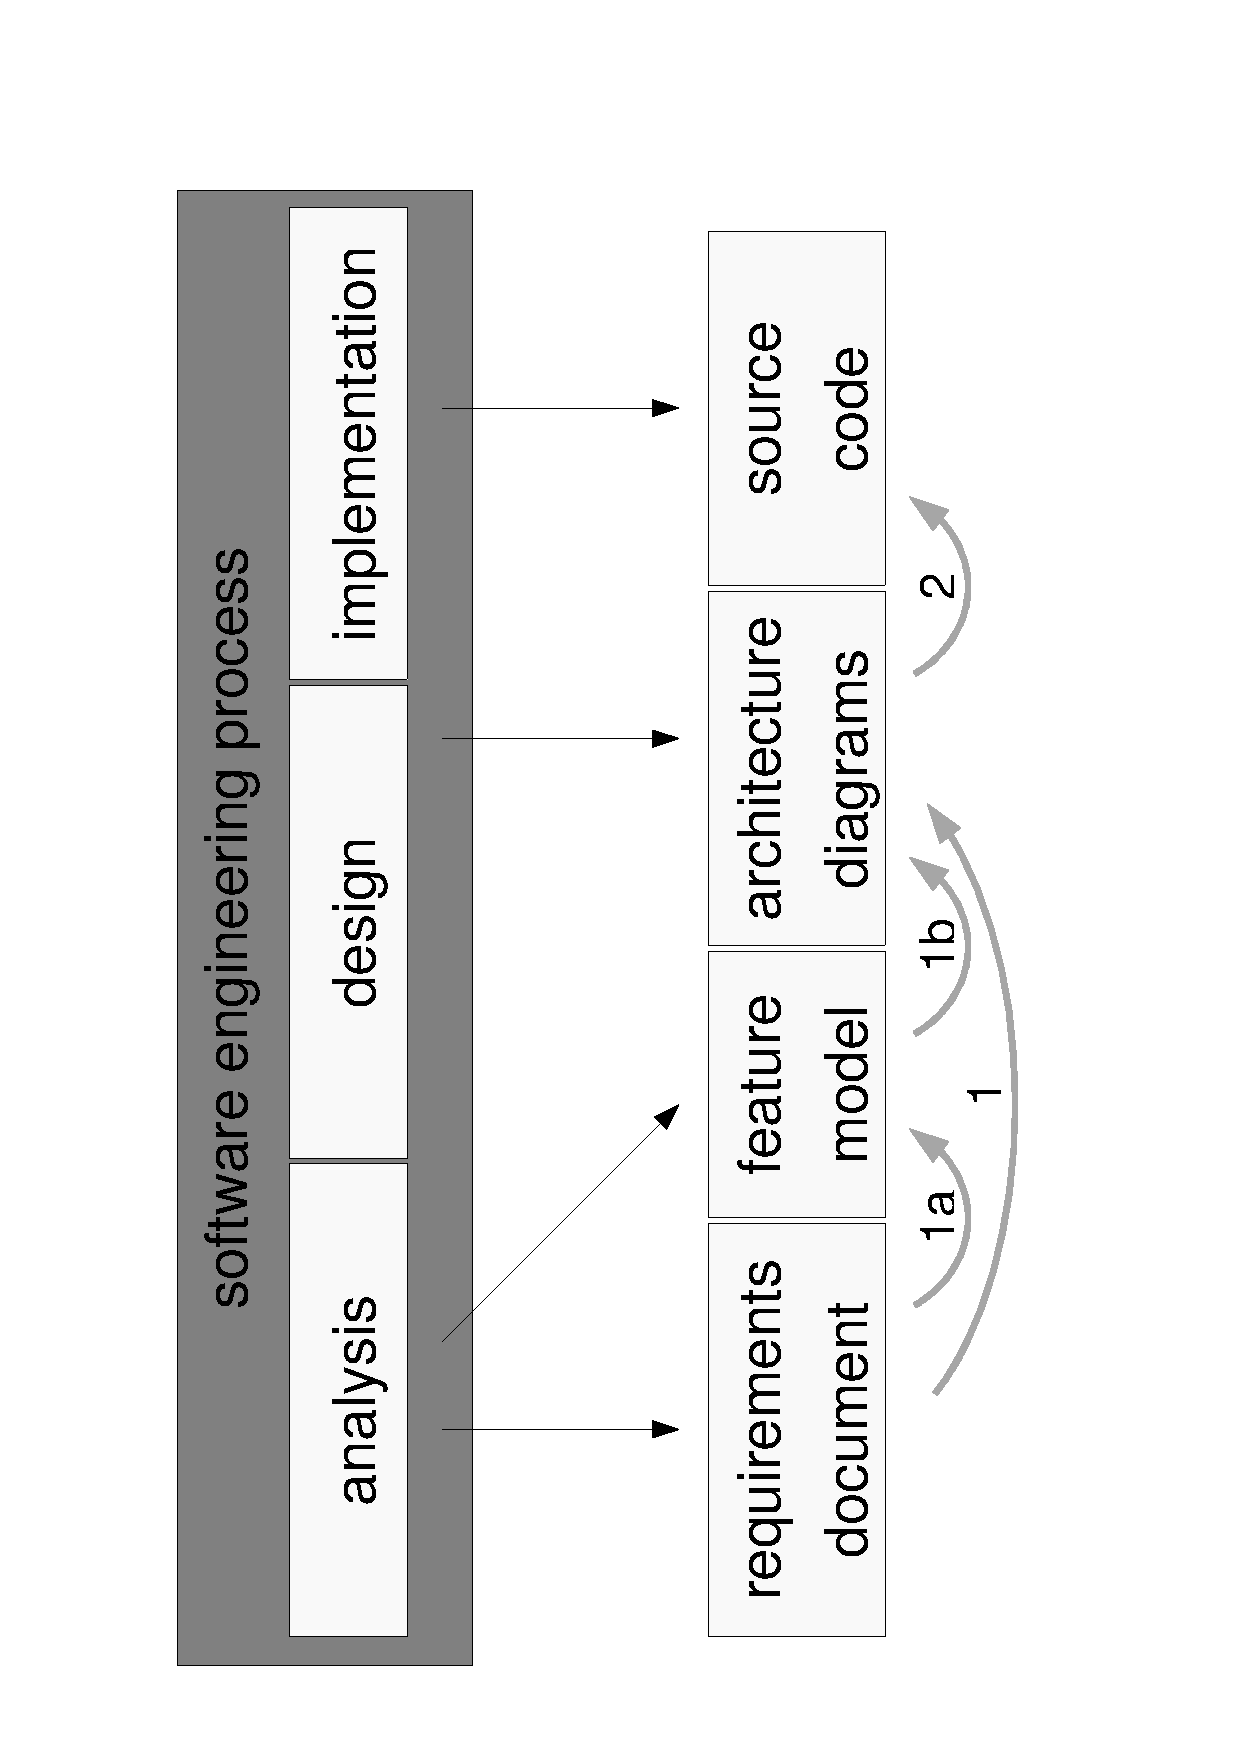
\includegraphics[scale=0.3,angle=-90]{graphics/gaps.pdf}
        \caption{Standard Software Engineering Process}
        \label{software_engineering_process_figure}
    \end{center}
\end{figure}

%
% $RCSfile: interpretation.tex,v $
%
% Copyright (c) 2002-2007. Christian Heller. All rights reserved.
%
% Permission is granted to copy, distribute and/or modify this document
% under the terms of the GNU Free Documentation License, Version 1.1 or
% any later version published by the Free Software Foundation; with no
% Invariant Sections, with no Front-Cover Texts and with no Back-Cover
% Texts. A copy of the license is included in the section entitled
% "GNU Free Documentation License".
%
% http://www.cybop.net
% - Cybernetics Oriented Programming -
%
% Version: $Revision: 1.1 $ $Date: 2007-07-17 20:02:36 $ $Author: christian $
% Authors: Christian Heller <christian.heller@tuxtax.de>
%

\subsection{Interpretation}
\label{inerpretation_heading}
\index{Interpretation}

CYBOP
CYBOL
CYBOI

\begin{figure}[ht]
    \begin{center}
        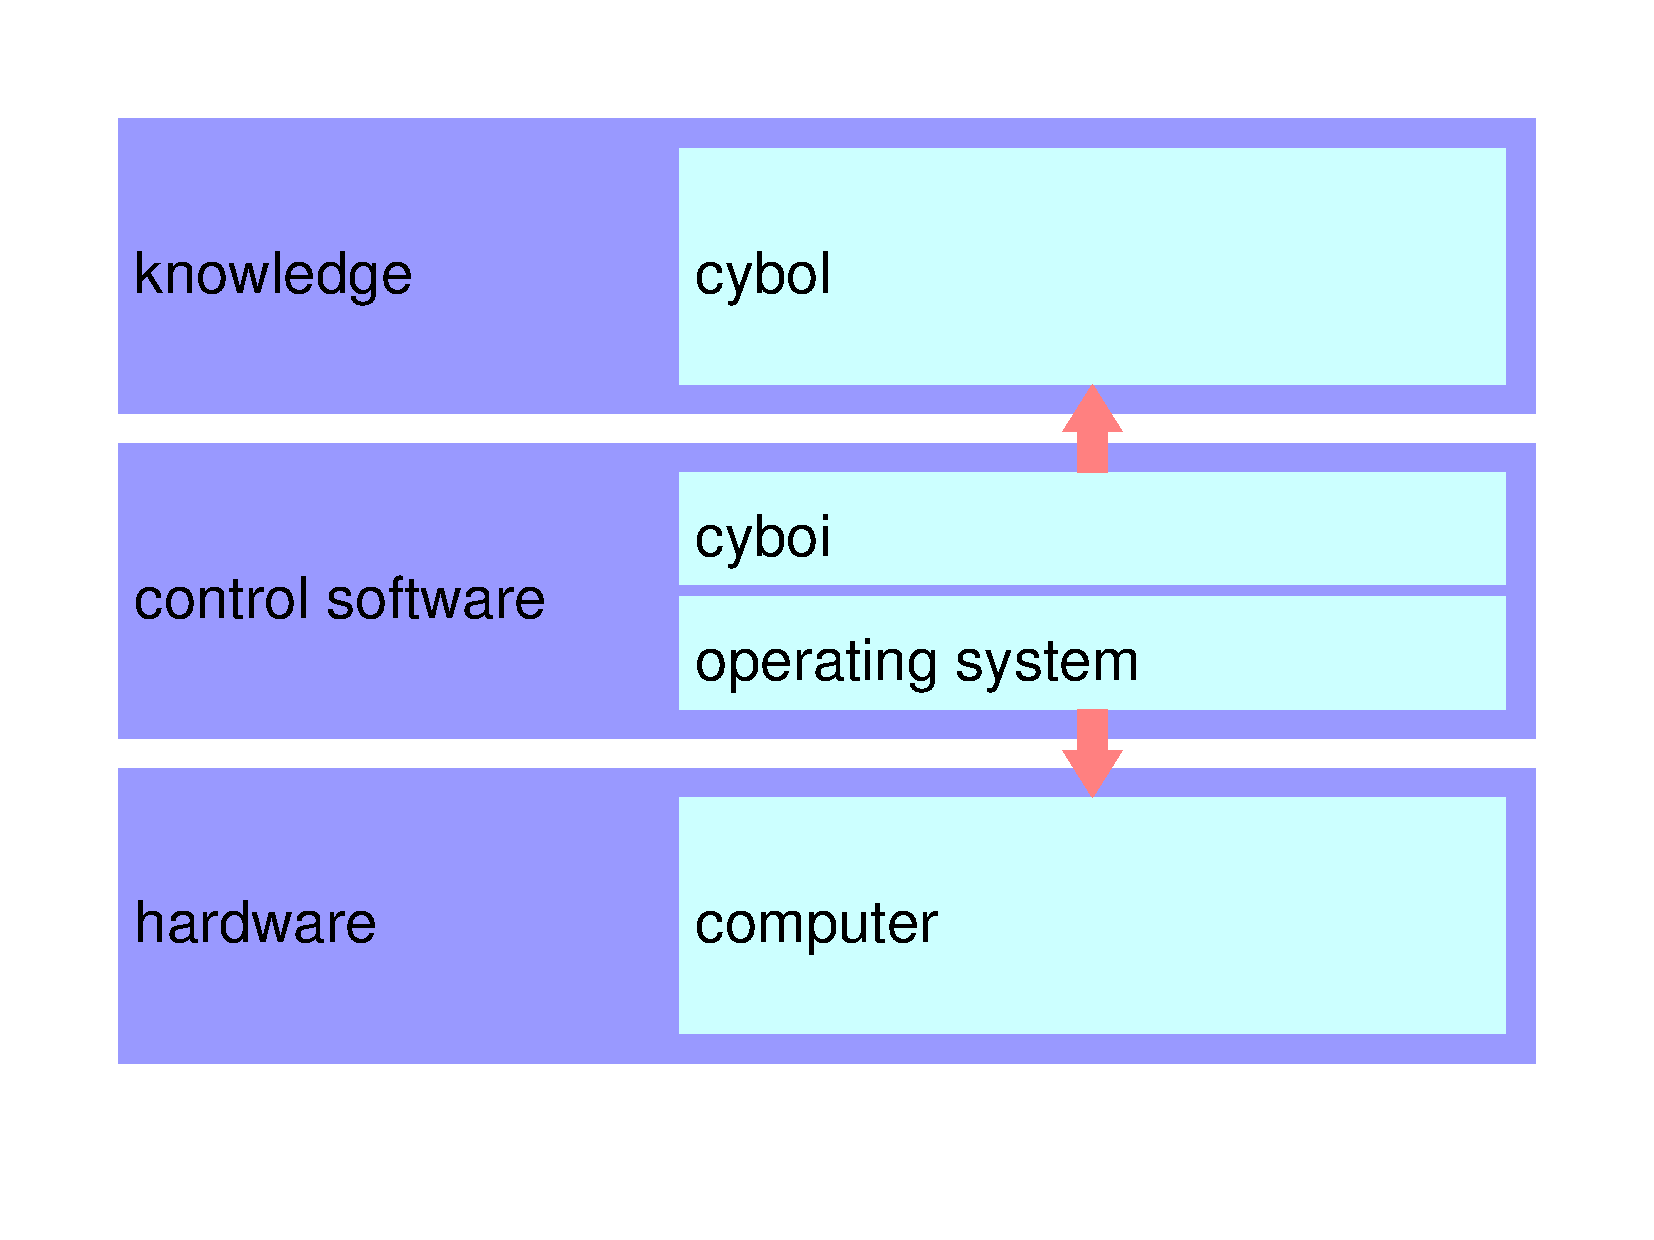
\includegraphics[scale=0.3,angle=-90]{graphics/connection.pdf}
        \caption{CYBOL Interpretation}
        \label{cybol_interpretation_figure}
    \end{center}
\end{figure}


%
% $RCSfile: extensible_markup_language.tex,v $
%
% Copyright (c) 2002-2007. Christian Heller. All rights reserved.
%
% Permission is granted to copy, distribute and/or modify this document
% under the terms of the GNU Free Documentation License, Version 1.1 or
% any later version published by the Free Software Foundation; with no
% Invariant Sections, with no Front-Cover Texts and with no Back-Cover
% Texts. A copy of the license is included in the section entitled
% "GNU Free Documentation License".
%
% http://www.cybop.net
% - Cybernetics Oriented Programming -
%
% Version: $Revision: 1.1 $ $Date: 2007-07-17 20:02:36 $ $Author: christian $
% Authors: Christian Heller <christian.heller@tuxtax.de>
%

\section{Extensible Markup Language}
\label{extensible_markup_language_heading}
\index{Extensible Markup Language}

The \emph{Extensible Markup Language} (XML) is ...


    \newpage{\pagestyle{empty}\cleardoublepage}
    %
% $RCSfile: definition.tex,v $
%
% Copyright (c) 2004. Christian Heller. All rights reserved.
%
% No copying, altering, distribution or any other actions concerning this
% document, except after explicit permission by the author!
% At some later point in time, this document is planned to be put under
% the GNU FDL license. For now, _everything_ is _restricted_ by the author.
%
% http://www.cybop.net
% - Cybernetics Oriented Programming -
%
% http://www.resmedicinae.org
% - Information in Medicine -
%
% @author Christian Heller <christian.heller@tuxtax.de>
%

\subsection{Definition}
\label{definition_heading}

\emph{Patterns}, in a more correct form called \emph{Software Patterns}, represent
solutions for recurring software design problems and can be understood as
recommendations for how to build software in an elegant way. In the past, more
detailed definitions have been given by meanwhile well-known authors.

Christopher Alexander, an architect and urban planner, writes \cite{alexander}:
\textit{Each pattern describes a problem which occurs over and over again in
our environment, and then describes the core of the solution to that problem,
in such a way that you can use this solution a million times over, without ever
doing it the same way twice.} He gave this definition primarily for problems
occuring in architecture, construction, and urban/regional planning, but it can
be applied in the same manner to software design, as done first by Ward
Cunningham and others \cite{portland}.

The systems designer Swift \cite{designmatrix} sees a pattern as:
\textit{essentially a morphological law, a relationship among parts (pattern
components) within a particular context. Specifically, a pattern expresses a
relationship among parts that resolves problems that would exist if the
relationship were missing. As patterns express these relationships, they are
not formulae or algorithms, but rather loose rules of thumb or heuristics.}

The \emph{Gang of Four} (Erich Gamma et al.) applied Alexander's definition to
object oriented software and created a whole catalogue of design patterns
\cite{gamma1995}. After them, patterns are: \textit{Structured models of
thinking that represent reusable solutions for one-and-the-same design problem.
They shall support the development, maintenance and extension of large software
systems, while being independent from concrete implementation languages.} The
experts identified four basic elements of each pattern: \emph{Name},
\emph{Problem}, \emph{Solution} and \emph{Consequences} (advantages and
disadvantages).

For Frank Buschmann et al., software patterns contain the knowledge of
experienced software engineers and help to improve the quality of decision
making \cite{buschmann}. In his opinion, they are \emph{Problem Solution Pairs},
that is basic solutions for problems that already occured in a similar way before.

Martin Fowler means that: \textit{A pattern is some idea that already was
helpful in a practical context and will probably be useful in other contexts,
too.} \cite{fowler1997}. After him, patterns, however they are written, have
four essential parts: \emph{Context}, \emph{Problem}, \emph{Forces} and
\emph{Solution}.

Depending on their experience, software developers produce good or bad solutions.
One possibility to improve less well-done designs or to extend legacy systems
are \emph{Anti-Patterns} (telling how to go from a problem to a bad design),
or the contrasting \emph{Amelioration Patterns} (telling how to go from a bad-
to a good solution) \cite{portland}. Both help finding patterns in wrong-designed
systems, to improve these.

There are efforts to combine patterns to form a \emph{Pattern Language}, also
called \emph{Pattern System} \cite{buschmann}. Such systems describe
dependencies between patterns, specify rules for pattern combination and show
how patterns can be implemented and used in software development practice.

    \newpage{\pagestyle{empty}\cleardoublepage}
    %
% $RCSfile: state_models.tex,v $
%
% Copyright (c) 2002-2007. Christian Heller. All rights reserved.
%
% Permission is granted to copy, distribute and/or modify this document
% under the terms of the GNU Free Documentation License, Version 1.1 or
% any later version published by the Free Software Foundation; with no
% Invariant Sections, with no Front-Cover Texts and with no Back-Cover
% Texts. A copy of the license is included in the section entitled
% "GNU Free Documentation License".
%
% http://www.cybop.net
% - Cybernetics Oriented Programming -
%
% Version: $Revision: 1.1 $ $Date: 2007-07-17 20:02:36 $ $Author: christian $
% Authors: Christian Heller <christian.heller@tuxtax.de>
%

\chapter{State Models}
\label{state_models_heading}
\index{State Models}

%
% $RCSfile: user_interface.tex,v $
%
% Copyright (c) 2002-2007. Christian Heller. All rights reserved.
%
% Permission is granted to copy, distribute and/or modify this document
% under the terms of the GNU Free Documentation License, Version 1.1 or
% any later version published by the Free Software Foundation; with no
% Invariant Sections, with no Front-Cover Texts and with no Back-Cover
% Texts. A copy of the license is included in the section entitled
% "GNU Free Documentation License".
%
% http://www.cybop.net
% - Cybernetics Oriented Programming -
%
% Version: $Revision: 1.2 $ $Date: 2007-08-01 13:59:01 $ $Author: christian $
% Authors: Christian Heller <christian.heller@tuxtax.de>
%

\section{User Interface}
\label{user_interface_heading}
\index{User Interface}

A \emph{User Interface} (UI) provides functionality by which a user can
communicate with a software system.

%
% $RCSfile: textual_user_interface.tex,v $
%
% Copyright (c) 2002-2007. Christian Heller. All rights reserved.
%
% Permission is granted to copy, distribute and/or modify this document
% under the terms of the GNU Free Documentation License, Version 1.1 or
% any later version published by the Free Software Foundation; with no
% Invariant Sections, with no Front-Cover Texts and with no Back-Cover
% Texts. A copy of the license is included in the section entitled
% "GNU Free Documentation License".
%
% http://www.cybop.net
% - Cybernetics Oriented Programming -
%
% Version: $Revision: 1.1 $ $Date: 2007-07-17 20:02:36 $ $Author: christian $
% Authors: Christian Heller <christian.heller@tuxtax.de>
%

\subsection{Textual User Interface}
\label{textual_user_interface_heading}
\index{Textual User Interface}

\emph{Textual User Interface} (TUI) is a synonym for character-based UI.
Historically, the TUI (besides the simple command line) was the first kind of
UI for computers. It mostly offers a menu with a list of possible choices that
can be activated via the pressing of a special button on the keyboard. Figure
\ref{textual_user_interface_figure} illustrates a typical, menu-based TUI.

\begin{figure}[ht]
    \begin{center}
%        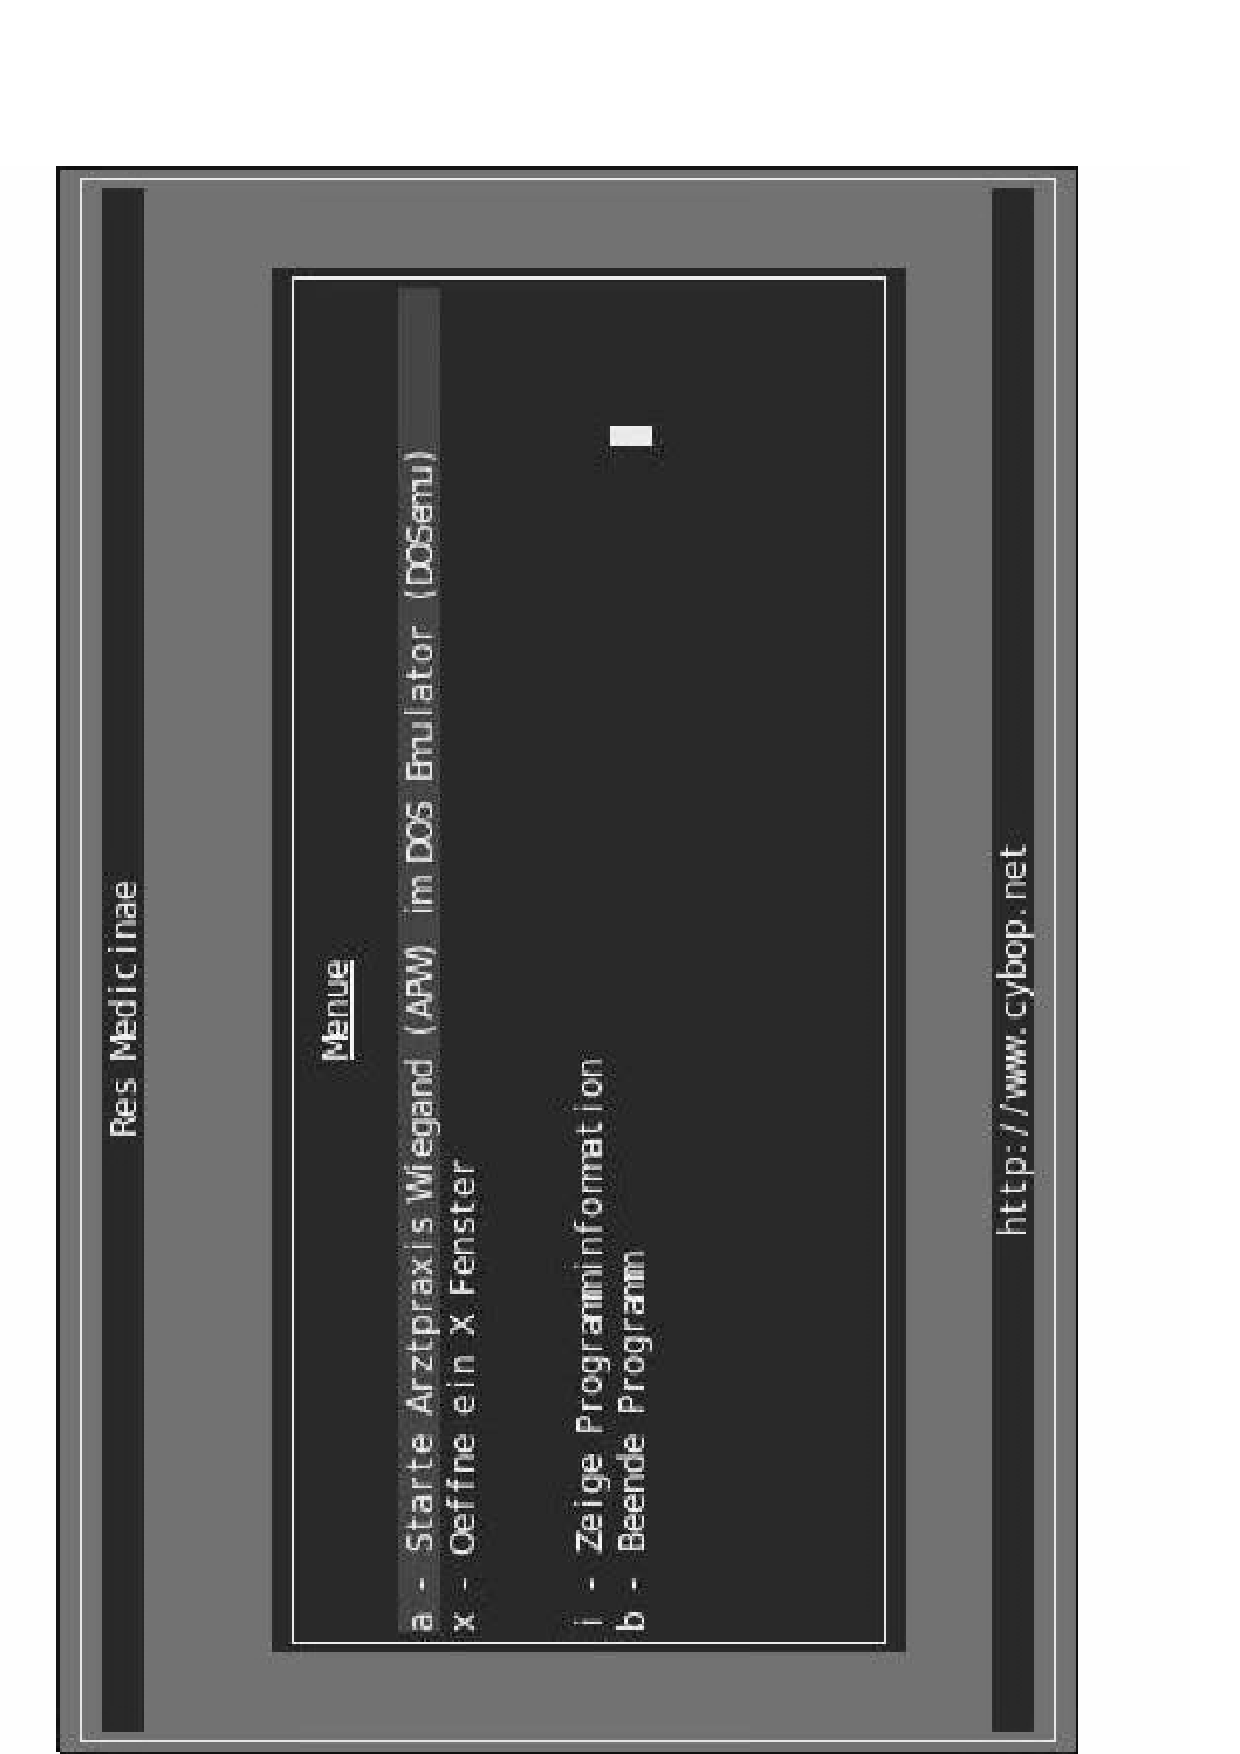
\includegraphics[scale=0.3,angle=-90]{graphics/textual_user_interface.pdf}
        \caption{Textual User Interface}
        \label{textual_user_interface_figure}
    \end{center}
\end{figure}

\subsubsection{Position Property}

\emph{required}

name=\texttt{'position'}\\
abstraction=\texttt{'integer'}\\
model=\texttt{x, y, z coordinates}

This property specifies the TUI element's origin.

\subsubsection{Size Property}

\emph{required}

name=\texttt{'size'}\\
abstraction=\texttt{'integer'}\\
model=\texttt{x, y, z extensions}

This property specifies the TUI element's extension.

\subsubsection{Background Property}

\emph{required}

name=\texttt{'background'}\\
abstraction=\texttt{'character'}\\
model=\texttt{'black' \vline\ 'red' \vline\ 'green' \vline\ 'yellow' \vline\ 'blue' \vline\ 'magenta' \vline\ 'cobalt' \vline\ 'white'}

This property specifies the background colour of the TUI.

\subsubsection{Foreground Property}

\emph{required}

name=\texttt{'foreground'}\\
abstraction=\texttt{'character'}\\
model=\texttt{'black' \vline\ 'red' \vline\ 'green' \vline\ 'yellow' \vline\ 'blue' \vline\ 'magenta' \vline\ 'cobalt' \vline\ 'white'}

This property specifies the foreground colour of the TUI.

\subsubsection{Border Property}

\emph{optional}

name=\texttt{'border'}\\
abstraction=\texttt{'character'}\\
model=\texttt{'line' \vline\ 'round\_line' \vline\ 'double\_line'}

This property specifies the kind of border of the TUI.

\subsubsection{Hidden Property}

\emph{optional}

name=\texttt{'hidden'}\\
abstraction=\texttt{'boolean'}\\
model=\texttt{'true' \vline\ 'false'}

This property specifies whether or not to hide the TUI element.

\subsubsection{Inverse Property}

\emph{optional}

name=\texttt{'inverse'}\\
abstraction=\texttt{'boolean'}\\
model=\texttt{'true' \vline\ 'false'}

This property specifies whether or not to display the TUI element in inverse
colours.

\subsubsection{Blink Property}

\emph{optional}

name=\texttt{'blink'}\\
abstraction=\texttt{'boolean'}\\
model=\texttt{'true' \vline\ 'false'}

This property specifies whether or not the TUI element should blink.

\subsubsection{Underline Property}

\emph{optional}

name=\texttt{'underline'}\\
abstraction=\texttt{'boolean'}\\
model=\texttt{'true' \vline\ 'false'}

This property specifies whether or not to underline the TUI element's text.

\subsubsection{Bold Property}

\emph{optional}

name=\texttt{'bold'}\\
abstraction=\texttt{'boolean'}\\
model=\texttt{'true' \vline\ 'false'}

This property specifies whether or not to display the TUI element's text in
bold font.

\subsubsection{Focus Property}

\emph{optional}, only if TUI element should be able to react to button press events

name=\texttt{'focus'}\\
abstraction=\texttt{'knowledge' \vline\ 'encapsulated'}\\
model=\texttt{logic knowledge model}

This property points to the TUI element (knowledge model) having focus. It is
important to find out which TUI element a key press event relates to. The focus
of a number of part elements should always be held by their corresponding
whole (compound) element.

\subsubsection{Previous Property}

\emph{optional}, only if TUI element should have a predecessor that may own the focus

name=\texttt{'previous'}\\
abstraction=\texttt{'knowledge' \vline\ 'encapsulated'}\\
model=\texttt{logic knowledge model}

This property points to the previous TUI element (knowledge model) owning focus.

\subsubsection{Next Property}

\emph{optional}, only if TUI element should have a successor that may own the focus

name=\texttt{'next'}\\
abstraction=\texttt{'knowledge' \vline\ 'encapsulated'}\\
model=\texttt{logic knowledge model}

This property points to the next TUI element (knowledge model) receiving focus.

\subsubsection{Enter Property}

\emph{optional}, only if TUI element should react to button press event;
a prerequisition is that the TUI element's \emph{focus} property value is \emph{true}

name=\texttt{'enter'}\\
abstraction=\texttt{'knowledge' \vline\ 'encapsulated'}\\
model=\texttt{logic knowledge model}

This property specifies the logic knowledge model to be executed if the
\emph{Enter} button is pressed while the TUI element has focus.

\subsubsection{Escape Property}

\emph{optional}, only if TUI element should react to button press event;
a prerequisition is that the TUI element's \emph{focus} property value is \emph{true}

name=\texttt{'escape'}\\
abstraction=\texttt{'knowledge' \vline\ 'encapsulated'}\\
model=\texttt{logic knowledge model}

This property specifies the logic knowledge model to be executed if the
\emph{Esc} button is pressed while the TUI element has focus.

\subsubsection{Arrow Up Property}

\emph{optional}, only if TUI element should react to button press event;
a prerequisition is that the TUI element's \emph{focus} property value is \emph{true}

name=\texttt{'arrow\_up'}\\
abstraction=\texttt{'knowledge' \vline\ 'encapsulated'}\\
model=\texttt{logic knowledge model}

This property specifies the logic knowledge model to be executed if the
\emph{arrow-up} button is pressed while the TUI element has focus.

\subsubsection{Arrow Down Property}

\emph{optional}, only if TUI element should react to button press event;
a prerequisition is that the TUI element's \emph{focus} property value is \emph{true}

name=\texttt{'arrow\_down'}\\
abstraction=\texttt{'knowledge' \vline\ 'encapsulated'}\\
model=\texttt{logic knowledge model}

This property specifies the logic knowledge model to be executed if the
\emph{arrow-down} button is pressed while the TUI element has focus.

\subsubsection{Arrow Left Property}

\emph{optional}, only if TUI element should react to button press event;
a prerequisition is that the TUI element's \emph{focus} property value is \emph{true}

name=\texttt{'arrow\_left'}\\
abstraction=\texttt{'knowledge' \vline\ 'encapsulated'}\\
model=\texttt{logic knowledge model}

This property specifies the logic knowledge model to be executed if the
\emph{arrow-left} button is pressed while the TUI element has focus.

\subsubsection{Arrow Right Property}

\emph{optional}, only if TUI element should react to button press event;
a prerequisition is that the TUI element's \emph{focus} property value is \emph{true}

name=\texttt{'arrow\_right'}\\
abstraction=\texttt{'knowledge' \vline\ 'encapsulated'}\\
model=\texttt{logic knowledge model}

This property specifies the logic knowledge model to be executed if the
\emph{arrow-right} button is pressed while the TUI element has focus.

%
% $RCSfile: graphical_user_interface.tex,v $
%
% Copyright (c) 2002-2007. Christian Heller. All rights reserved.
%
% Permission is granted to copy, distribute and/or modify this document
% under the terms of the GNU Free Documentation License, Version 1.1 or
% any later version published by the Free Software Foundation; with no
% Invariant Sections, with no Front-Cover Texts and with no Back-Cover
% Texts. A copy of the license is included in the section entitled
% "GNU Free Documentation License".
%
% http://www.cybop.net
% - Cybernetics Oriented Programming -
%
% Version: $Revision: 1.1 $ $Date: 2007-07-17 20:02:36 $ $Author: christian $
% Authors: Christian Heller <christian.heller@tuxtax.de>
%

\subsection{Graphical User Interface}
\label{graphical_user_interface_heading}
\index{Graphical User Interface}

A \emph{Graphical User Interface} (GUI) is mostly based on so-called graphical
\emph{Windows} which may overlap, or be ordered side-by-side on a screen.
Figure \ref{graphical_user_interface_figure} illustrates a typical GUI.

\begin{figure}[ht]
    \begin{center}
%        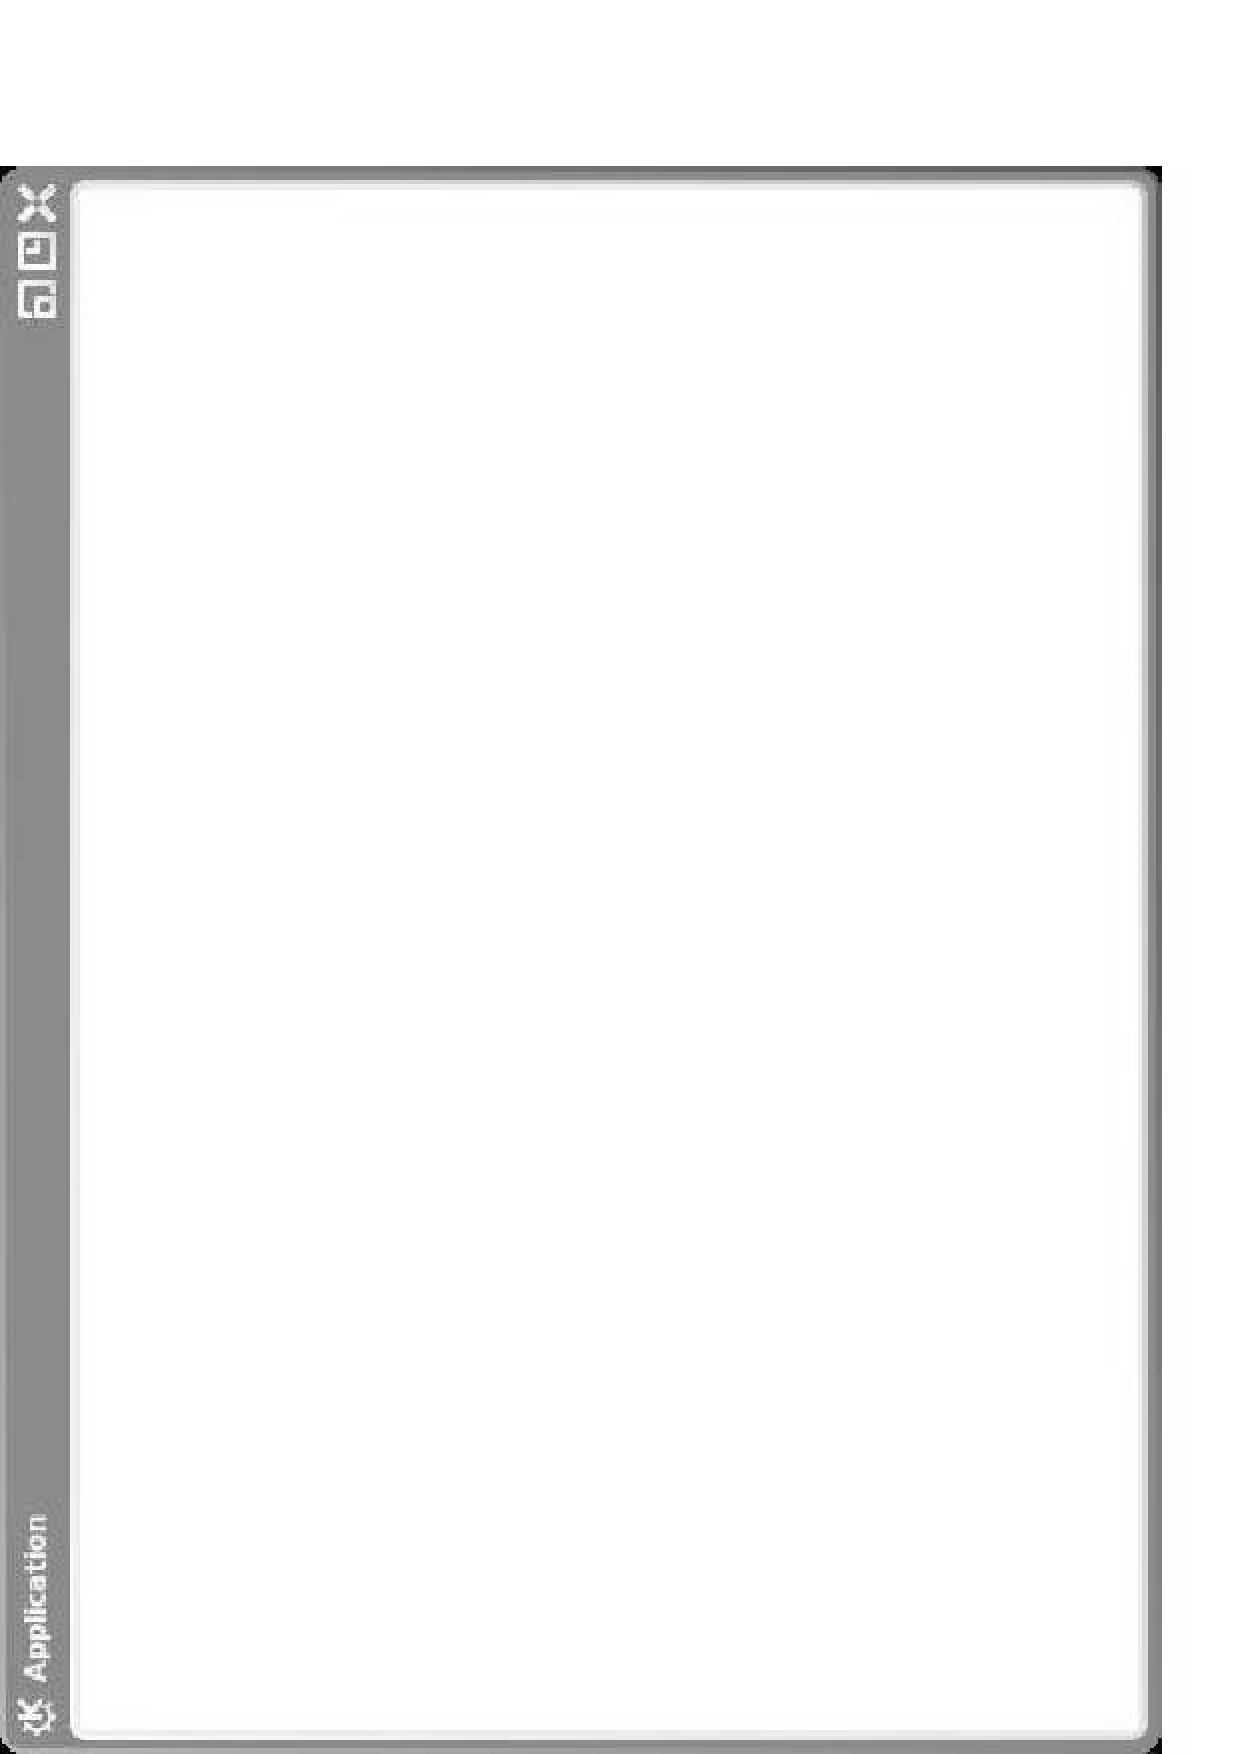
\includegraphics[scale=0.3,angle=-90]{graphics/graphical_user_interface.pdf}
        \caption{Graphical User Interface}
        \label{graphical_user_interface_figure}
    \end{center}
\end{figure}

\subsubsection{Shape Property}

\emph{required}

name=\texttt{'shape'}\\
abstraction=\texttt{'character'}\\
model=\texttt{'rectangle' \vline\ 'circle' \vline\ 'polygon'}

This property specifies the geometrical shape of the GUI.

\subsubsection{Layout Property}

\emph{required}

name=\texttt{'layout'}\\
abstraction=\texttt{'character'}\\
model=\texttt{'root' \vline\ 'coordinates' \vline\ 'compass'}

This property specifies the kind of layout of the GUI.

\subsubsection{Cell Property}

\emph{optional}, only if \emph{layout} property is \emph{compass}

name=\texttt{'cell'}\\
abstraction=\texttt{'character'}\\
model=\texttt{'north' \vline\ 'south' \vline\ 'west' \vline\ 'east' \vline\ 'centre'}

This property specifies the cell ordering, if \emph{compass} layout is used.

\subsubsection{Position Property}

\emph{required}

name=\texttt{'position'}\\
abstraction=\texttt{'integer'}\\
model=\texttt{x, y, z coordinates}

This property specifies the GUI element's origin.

\subsubsection{Size Property}

\emph{required}

name=\texttt{'size'}\\
abstraction=\texttt{'integer'}\\
model=\texttt{x, y, z extensions}

This property specifies the GUI element's extension.

\subsubsection{Background Property}

\emph{optional}

name=\texttt{'background'}\\
abstraction=\texttt{'character'}\\
model=\texttt{'black' \vline\ 'red' \vline\ 'green' \vline\ 'yellow' \vline\ 'blue' \vline\ 'magenta' \vline\ 'cobalt' \vline\ 'white'}

This property specifies the background colour of the GUI.

\subsubsection{Foreground Property}

\emph{optional}

name=\texttt{'foreground'}\\
abstraction=\texttt{'character'}\\
model=\texttt{'black' \vline\ 'red' \vline\ 'green' \vline\ 'yellow' \vline\ 'blue' \vline\ 'magenta' \vline\ 'cobalt' \vline\ 'white'}

This property specifies the foreground colour of the GUI.

\subsubsection{Title Property}

\emph{optional}, only if \emph{layout} property is \emph{root}

name=\texttt{'title'}\\
abstraction=\texttt{'character'}\\
model=\texttt{window title}

This property specifies the GUI element's (window's) title.

\subsubsection{Icon Property}

\emph{optional}, only if \emph{layout} property is \emph{root}

name=\texttt{'icon'}\\
abstraction=\texttt{'bmp' \vline\ 'jpeg' \vline\ 'png' \vline\ 'gif' \vline\ etc.}\\
model=\texttt{graphic file}

This property specifies the GUI element's (window's) icon.

\subsubsection{Expose Property}

\emph{optional}, only if GUI element should react to expose event

name=\texttt{'expose'}\\
abstraction=\texttt{'knowledge' \vline\ 'encapsulated'}\\
model=\texttt{logic knowledge model}

This property specifies the logic knowledge model to be executed if the GUI
element is exposed, for example shown again after having been hidden before.

\subsubsection{Mouse Over Property}

\emph{optional}, only if GUI element should react to mouse event

name=\texttt{'mouse\_over'}\\
abstraction=\texttt{'knowledge' \vline\ 'encapsulated'}\\
model=\texttt{logic knowledge model}

This property specifies the logic knowledge model to be executed if the mouse
is moved over the GUI element.

\subsubsection{Mouse Wheel Property}

\emph{optional}, only if GUI element should react to mouse event

name=\texttt{'mouse\_wheel'}\\
abstraction=\texttt{'knowledge' \vline\ 'encapsulated'}\\
model=\texttt{logic knowledge model}

This property specifies the logic knowledge model to be executed if the mouse
wheel is scrolled while the mouse pointer is over the GUI element.

\subsubsection{Left Press Property}

\emph{optional}, only if GUI element should react to mouse event

name=\texttt{'left\_press'}\\
abstraction=\texttt{'knowledge' \vline\ 'encapsulated'}\\
model=\texttt{logic knowledge model}

This property specifies the logic knowledge model to be executed if the left
mouse button is pressed.

\subsubsection{Left Release Property}

\emph{optional}, only if GUI element should react to mouse event

name=\texttt{'left\_release'}\\
abstraction=\texttt{'knowledge' \vline\ 'encapsulated'}\\
model=\texttt{logic knowledge model}

This property specifies the logic knowledge model to be executed if the left
mouse button is released.

\subsubsection{Left Click Property}

\emph{optional}, only if GUI element should react to mouse event

name=\texttt{'left\_click'}\\
abstraction=\texttt{'knowledge' \vline\ 'encapsulated'}\\
model=\texttt{logic knowledge model}

This property specifies the logic knowledge model to be executed if the left
mouse button is clicked. A mouse click is the combination of a mouse press- and
release event.

%
% $RCSfile: web_user_interface.tex,v $
%
% Copyright (c) 2002-2007. Christian Heller. All rights reserved.
%
% Permission is granted to copy, distribute and/or modify this document
% under the terms of the GNU Free Documentation License, Version 1.1 or
% any later version published by the Free Software Foundation; with no
% Invariant Sections, with no Front-Cover Texts and with no Back-Cover
% Texts. A copy of the license is included in the section entitled
% "GNU Free Documentation License".
%
% http://www.cybop.net
% - Cybernetics Oriented Programming -
%
% Version: $Revision: 1.2 $ $Date: 2007-08-01 13:59:01 $ $Author: christian $
% Authors: Christian Heller <christian.heller@tuxtax.de>
%

\subsection{Web User Interface}
\label{web_user_interface_heading}
\index{Web User Interface}

A \emph{Web User Interface} (WUI) is what is commonly also known as
\emph{Hypertext Markup Language} (HTML) file. HTML files get interpreted by a
\emph{Web Browser} which renders the graphical and textual information to
display these as HTML page. Figure \ref{web_user_interface_figure} shows an
example WUI.

\begin{figure}[ht]
    \begin{center}
        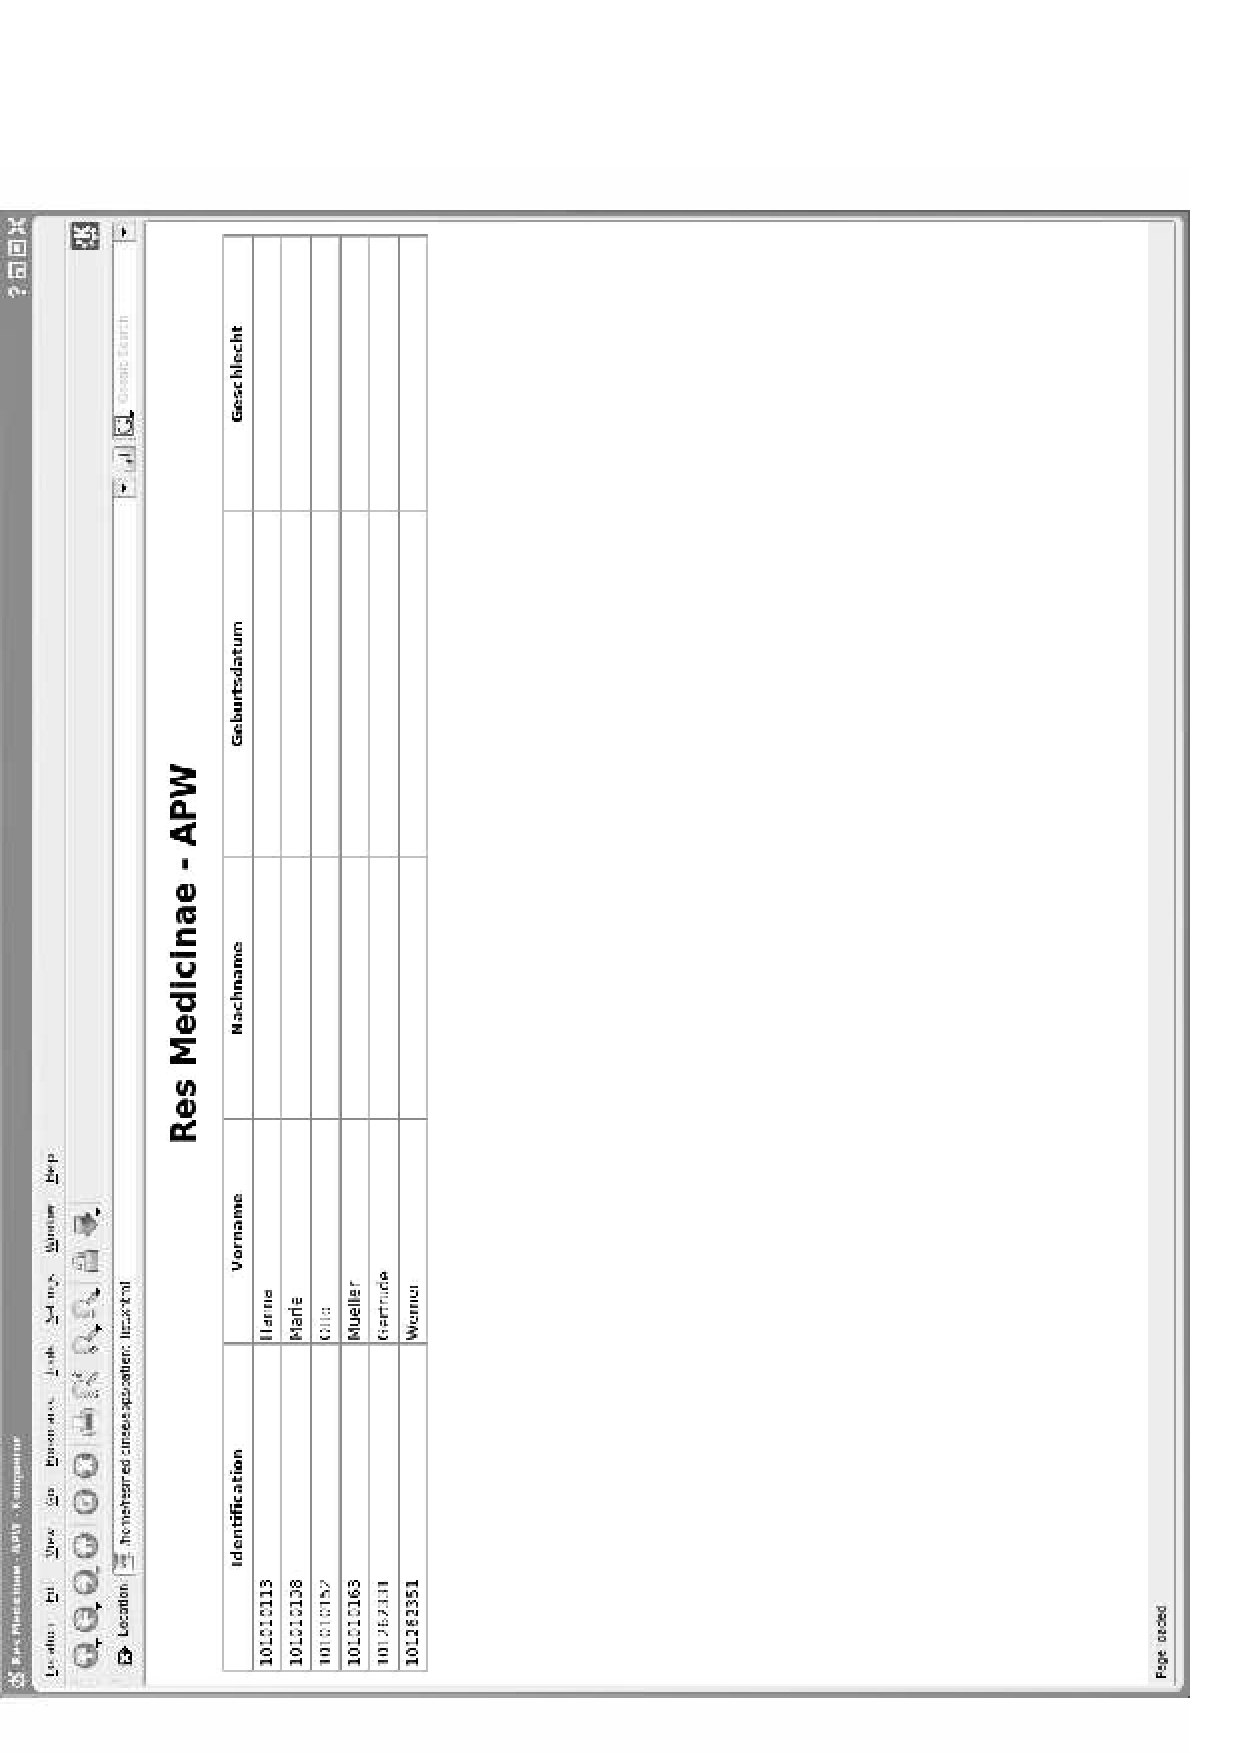
\includegraphics[scale=0.3,angle=-90]{graphics/web_user_interface.pdf}
        \caption{Web User Interface}
        \label{web_user_interface_figure}
    \end{center}
\end{figure}

\subsubsection{Example}

\begin{scriptsize}
    \begin{verbatim}
<part name="address_table" channel="file" abstraction="compound" model="wui/table.cybol">
    <property name="tag" channel="inline" abstraction="character" model="table"/>
    <property name="width" channel="inline" abstraction="character" model="100%"/>
    <property name="cellspacing" channel="inline" abstraction="integer" model="5"/>
    <property name="cellpadding" channel="inline" abstraction="integer" model="2"/>
    <property name="border" channel="inline" abstraction="boolean" model="false"/>
</part>
    \end{verbatim}
\end{scriptsize}

\subsubsection{Tag Property}

This property specifies the HTML tag to associate with the knowledge model.

\emph{required}

name=\texttt{'tag'}\\
abstraction=\texttt{'character'}\\
model=\texttt{'html' \vline\ 'head' \vline\ 'meta' \vline\ 'body' \vline\ 'table' \vline\ 'tr' \vline\ etc.}

\subsubsection{Xmlns Property}

This property specifies the XML namespace for the HTML page to be generated
from the WUI.

\emph{optional}, only for \emph{html} tag

name=\texttt{'xmlns'}\\
abstraction=\texttt{'character'}\\
model=\texttt{'http://www.w3.org/1999/xhtml'}

\subsubsection{HTTP-Equiv Property}

This property specifies the content type for the HTML page to be generated from
the WUI.

\emph{optional}, only for \emph{meta} tag

name=\texttt{'http-equiv'}\\
abstraction=\texttt{'character'}\\
model=\texttt{'content-type'}

\subsubsection{Name Property}

This property specifies the name of a meta data entry for the HTML page to be
generated from the WUI.

\emph{optional}, only for \emph{meta} tag

name=\texttt{'name'}\\
abstraction=\texttt{'character'}\\
model=\texttt{'author'}

\subsubsection{Content Property}

This property specifies the content of a meta data entry for the HTML page to
be generated from the WUI.

\emph{optional}, only for \emph{meta} tag

name=\texttt{'content'}\\
abstraction=\texttt{'character'}\\
model=\texttt{'Generated by CYBOI'}

\subsubsection{Align Property}

This property specifies the alignment of the HTML heading.

\emph{optional}, only for \emph{h1..6} tag

name=\texttt{'align'}\\
abstraction=\texttt{'character'}\\
model=\texttt{'left' \vline\ 'right' \vline\ 'center'}

\subsubsection{Width Property}

This property specifies the width of the HTML table.

\emph{optional}, only for \emph{table} tag

name=\texttt{'width'}\\
abstraction=\texttt{'character'}\\
model=\texttt{table width}

\subsubsection{Cellspacing Property}

This property specifies the spacing between the cells of the HTML table.

\emph{optional}, only for \emph{table} tag

name=\texttt{'cellspacing'}\\
abstraction=\texttt{'character'}\\
model=\texttt{space between cells in pixels}

\subsubsection{Cellpadding Property}

This property specifies the space between an HTML table cell's border and its
content.

\emph{optional}, only for \emph{table} tag

name=\texttt{'cellpadding'}\\
abstraction=\texttt{'character'}\\
model=\texttt{space between cell border and content}

\subsubsection{Border Property}

This property specifies the width of the HTML table's border.

\emph{optional}, only for \emph{table} tag

name=\texttt{'border'}\\
abstraction=\texttt{'character'}\\
model=\texttt{table border width}

\subsubsection{HRef Property}

This property specifies the reference (link) to be invoked when activating the
HTML element.

\emph{optional}, only for \emph{a} tag

name=\texttt{'href'}\\
abstraction=\texttt{'character'}\\
model=\texttt{an HTML reference}



%\input{three_dimensional_graphic}
%\input{vector_graphic}
%%
% $RCSfile: document.tex,v $
%
% Copyright (c) 2002-2007. Christian Heller. All rights reserved.
%
% Permission is granted to copy, distribute and/or modify this document
% under the terms of the GNU Free Documentation License, Version 1.1 or
% any later version published by the Free Software Foundation; with no
% Invariant Sections, with no Front-Cover Texts and with no Back-Cover
% Texts. A copy of the license is included in the section entitled
% "GNU Free Documentation License".
%
% http://www.cybop.net
% - Cybernetics Oriented Programming -
%
% Version: $Revision: 1.1 $ $Date: 2007-08-01 13:59:00 $ $Author: christian $
% Authors: Christian Heller <christian.heller@tuxtax.de>
%

\section{Document}
\label{document_heading}
\index{Document}

A \emph{Document} can be structured in various ways and also its layout may
differ greatly. The CYBOL language provides a way to express both, structure
and layout of a document. The resulting knowledge model may be exported to
\latex, for example, to generate the document in different file formats.

\input{latex}
 (like LaTeX etc.)

% General cybol names.
%SUPER-PROPERTIES

    \newpage{\pagestyle{empty}\cleardoublepage}
    %
% $RCSfile: logic_models.tex,v $
%
% Copyright (c) 2002-2007. Christian Heller. All rights reserved.
%
% Permission is granted to copy, distribute and/or modify this document
% under the terms of the GNU Free Documentation License, Version 1.1 or
% any later version published by the Free Software Foundation; with no
% Invariant Sections, with no Front-Cover Texts and with no Back-Cover
% Texts. A copy of the license is included in the section entitled
% "GNU Free Documentation License".
%
% http://www.cybop.net
% - Cybernetics Oriented Programming -
%
% Version: $Revision: 1.1 $ $Date: 2007-07-17 20:02:36 $ $Author: christian $
% Authors: Christian Heller <christian.heller@tuxtax.de>
%

\chapter{Logic Models}
\label{logic_models_heading}
\index{Logic Models}

%
% $RCSfile: bit_manipulation.tex,v $
%
% Copyright (c) 2002-2007. Christian Heller. All rights reserved.
%
% Permission is granted to copy, distribute and/or modify this document
% under the terms of the GNU Free Documentation License, Version 1.1 or
% any later version published by the Free Software Foundation; with no
% Invariant Sections, with no Front-Cover Texts and with no Back-Cover
% Texts. A copy of the license is included in the section entitled
% "GNU Free Documentation License".
%
% http://www.cybop.net
% - Cybernetics Oriented Programming -
%
% Version: $Revision: 1.1 $ $Date: 2007-07-17 20:02:36 $ $Author: christian $
% Authors: Christian Heller <christian.heller@tuxtax.de>
%

\section{Bit Manipulation}
\label{bit_manipulation_heading}
\index{Bit Manipulation}

%
% $RCSfile: shift.tex,v $
%
% Copyright (c) 2002-2007. Christian Heller. All rights reserved.
%
% Permission is granted to copy, distribute and/or modify this document
% under the terms of the GNU Free Documentation License, Version 1.1 or
% any later version published by the Free Software Foundation; with no
% Invariant Sections, with no Front-Cover Texts and with no Back-Cover
% Texts. A copy of the license is included in the section entitled
% "GNU Free Documentation License".
%
% http://www.cybop.net
% - Cybernetics Oriented Programming -
%
% Version: $Revision: 1.1 $ $Date: 2007-07-17 20:02:36 $ $Author: christian $
% Authors: Christian Heller <christian.heller@tuxtax.de>
%

\subsection{Shift}
\label{shift_heading}
\index{Shift}

This operation shifts the bits within the number by the given positions.

\subsubsection{Number Property}

\emph{required}

name=\texttt{'number'}\\
abstraction=\texttt{'integer' \vline\ 'knowledge' \vline\ 'encapsulated'}\\
model=\texttt{the actual number (or knowledge model)}

This property specifies the number whose bits are to be shifted.

\subsubsection{Direction Property}

\emph{required}

name=\texttt{'direction'}\\
abstraction=\texttt{'character'}\\
model=\texttt{'left' \vline\ 'right'}

The direction in which to shift.

\subsubsection{Position Property}

\emph{required}

name=\texttt{'position'}\\
abstraction=\texttt{'integer' \vline\ 'knowledge' \vline\ 'encapsulated'}\\
model=\texttt{number of positions to shift by}

The number of positions by which the bits of the given number are to be shifted.

\subsubsection{Result Property}

\emph{required}

name=\texttt{'result'}\\
abstraction=\texttt{'knowledge' \vline\ 'encapsulated'}\\
model=\texttt{result knowledge model}

This is the result knowledge model in which to store the number whose bits were
shifted.

%
% $RCSfile: rotate.tex,v $
%
% Copyright (c) 2002-2007. Christian Heller. All rights reserved.
%
% Permission is granted to copy, distribute and/or modify this document
% under the terms of the GNU Free Documentation License, Version 1.1 or
% any later version published by the Free Software Foundation; with no
% Invariant Sections, with no Front-Cover Texts and with no Back-Cover
% Texts. A copy of the license is included in the section entitled
% "GNU Free Documentation License".
%
% http://www.cybop.net
% - Cybernetics Oriented Programming -
%
% Version: $Revision: 1.1 $ $Date: 2007-07-17 20:02:36 $ $Author: christian $
% Authors: Christian Heller <christian.heller@tuxtax.de>
%

\subsection{Rotate}
\label{rotate_heading}
\index{Rotate}

This operation rotates the bits within the number by the given positions.

\subsubsection{Number Property}

\emph{required}

name=\texttt{'number'}\\
abstraction=\texttt{'integer' \vline\ 'knowledge' \vline\ 'encapsulated'}\\
model=\texttt{the actual number (or knowledge model)}

This property specifies the number whose bits are to be rotated.

\subsubsection{Direction Property}

\emph{required}

name=\texttt{'direction'}\\
abstraction=\texttt{'character'}\\
model=\texttt{'left' \vline\ 'right'}

The direction in which to rotate.

\subsubsection{Position Property}

\emph{required}

name=\texttt{'position'}\\
abstraction=\texttt{'integer' \vline\ 'knowledge' \vline\ 'encapsulated'}\\
model=\texttt{number of positions to rotate by}

The number of positions by which the bits of the given number are to be rotated.

\subsubsection{Result Property}

\emph{required}

name=\texttt{'result'}\\
abstraction=\texttt{'knowledge' \vline\ 'encapsulated'}\\
model=\texttt{result knowledge model}

This is the result knowledge model in which to store the number whose bits were
rotated.

%
% $RCSfile: set_bit.tex,v $
%
% Copyright (c) 2002-2007. Christian Heller. All rights reserved.
%
% Permission is granted to copy, distribute and/or modify this document
% under the terms of the GNU Free Documentation License, Version 1.1 or
% any later version published by the Free Software Foundation; with no
% Invariant Sections, with no Front-Cover Texts and with no Back-Cover
% Texts. A copy of the license is included in the section entitled
% "GNU Free Documentation License".
%
% http://www.cybop.net
% - Cybernetics Oriented Programming -
%
% Version: $Revision: 1.2 $ $Date: 2007-08-01 13:59:00 $ $Author: christian $
% Authors: Christian Heller <christian.heller@tuxtax.de>
%

\subsection{Set Bit}
\label{set_bit_heading}
\index{Set Bit}

This operation sets the bit at the given position within the given number.
\emph{Set} means setting the bit to \emph{true}.

\subsubsection{Example}

\begin{scriptsize}
    \begin{verbatim}
<part name="set_some_bit" channel="inline" abstraction="operation" model="set_bit">
    <property name="number" channel="inline" abstraction="knowledge" model=".app.number"/>
    <property name="position" channel="inline" abstraction="knowledge" model=".app.pos"/>
    <property name="result" channel="inline" abstraction="knowledge" model=".app.result"/>
</part>
    \end{verbatim}
\end{scriptsize}

\subsubsection{Number Property}

This property specifies the number of which one bit is to be set.

\emph{required}

name=\texttt{'number'}\\
abstraction=\texttt{'integer' \vline\ 'knowledge' \vline\ 'encapsulated'}\\
model=\texttt{the actual number (or knowledge model)}

\subsubsection{Position Property}

The position of the bit whose value is to be set (set to \emph{true}).

\emph{required}

name=\texttt{'position'}\\
abstraction=\texttt{'integer' \vline\ 'knowledge' \vline\ 'encapsulated'}\\
model=\texttt{position of the bit}

\subsubsection{Result Property}

This is the result knowledge model in which to store the number of which one
bit was set (to \emph{true}).

\emph{required}

name=\texttt{'result'}\\
abstraction=\texttt{'knowledge' \vline\ 'encapsulated'}\\
model=\texttt{result knowledge model}

%
% $RCSfile: reset_bit.tex,v $
%
% Copyright (c) 2002-2007. Christian Heller. All rights reserved.
%
% Permission is granted to copy, distribute and/or modify this document
% under the terms of the GNU Free Documentation License, Version 1.1 or
% any later version published by the Free Software Foundation; with no
% Invariant Sections, with no Front-Cover Texts and with no Back-Cover
% Texts. A copy of the license is included in the section entitled
% "GNU Free Documentation License".
%
% http://www.cybop.net
% - Cybernetics Oriented Programming -
%
% Version: $Revision: 1.1 $ $Date: 2007-07-17 20:02:36 $ $Author: christian $
% Authors: Christian Heller <christian.heller@tuxtax.de>
%

\subsection{Reset Bit}
\label{reset_bit_heading}
\index{Reset Bit}

This operation resets the bit at the given position within the given number.
RESET means setting the bit to FALSE.

\subsubsection{Number Property}

\emph{required}

name=\texttt{'number'}\\
abstraction=\texttt{'integer' \vline\ 'knowledge' \vline\ 'encapsulated'}\\
model=\texttt{the actual number (or knowledge model)}

This property specifies the number of which one bit is to be reset.

\subsubsection{Position Property}

\emph{required}

name=\texttt{'position'}\\
abstraction=\texttt{'integer' \vline\ 'knowledge' \vline\ 'encapsulated'}\\
model=\texttt{position of the bit}

The position of the bit whose value is to be reset (set to FALSE).

\subsubsection{Result Property}

\emph{required}

name=\texttt{'result'}\\
abstraction=\texttt{'knowledge' \vline\ 'encapsulated'}\\
model=\texttt{result knowledge model}

This is the result knowledge model in which to store the number of which one
bit was reset.

%
% $RCSfile: get_bit.tex,v $
%
% Copyright (c) 2002-2007. Christian Heller. All rights reserved.
%
% Permission is granted to copy, distribute and/or modify this document
% under the terms of the GNU Free Documentation License, Version 1.1 or
% any later version published by the Free Software Foundation; with no
% Invariant Sections, with no Front-Cover Texts and with no Back-Cover
% Texts. A copy of the license is included in the section entitled
% "GNU Free Documentation License".
%
% http://www.cybop.net
% - Cybernetics Oriented Programming -
%
% Version: $Revision: 1.1 $ $Date: 2007-07-17 20:02:36 $ $Author: christian $
% Authors: Christian Heller <christian.heller@tuxtax.de>
%

\subsection{Get Bit}
\label{get_bit_heading}
\index{Get Bit}

This operation retrieves the bit at the given position, within the given number.

\subsubsection{Number Property}

\emph{required}

name=\texttt{'number'}\\
abstraction=\texttt{'integer' \vline\ 'knowledge' \vline\ 'encapsulated'}\\
model=\texttt{the actual number (or knowledge model)}

This property specifies the number of which one bit is to be retrieved.

\subsubsection{Position Property}

\emph{required}

name=\texttt{'position'}\\
abstraction=\texttt{'integer' \vline\ 'knowledge' \vline\ 'encapsulated'}\\
model=\texttt{position of the bit}

The position of the bit whose value is to be retrieved.

\subsubsection{Result Property}

\emph{required}

name=\texttt{'result'}\\
abstraction=\texttt{'knowledge' \vline\ 'encapsulated'}\\
model=\texttt{result knowledge model}

This is the result knowledge model in which to store the value of the bit that
was retrieved from the given number.


%
% $RCSfile: boolean_logic.tex,v $
%
% Copyright (c) 2002-2007. Christian Heller. All rights reserved.
%
% Permission is granted to copy, distribute and/or modify this document
% under the terms of the GNU Free Documentation License, Version 1.1 or
% any later version published by the Free Software Foundation; with no
% Invariant Sections, with no Front-Cover Texts and with no Back-Cover
% Texts. A copy of the license is included in the section entitled
% "GNU Free Documentation License".
%
% http://www.cybop.net
% - Cybernetics Oriented Programming -
%
% Version: $Revision: 1.1 $ $Date: 2007-07-17 20:02:36 $ $Author: christian $
% Authors: Christian Heller <christian.heller@tuxtax.de>
%

\section{Boolean Logic}
\label{boolean_logic_heading}
\index{Boolean Logic}

%
% $RCSfile: not.tex,v $
%
% Copyright (c) 2002-2007. Christian Heller. All rights reserved.
%
% Permission is granted to copy, distribute and/or modify this document
% under the terms of the GNU Free Documentation License, Version 1.1 or
% any later version published by the Free Software Foundation; with no
% Invariant Sections, with no Front-Cover Texts and with no Back-Cover
% Texts. A copy of the license is included in the section entitled
% "GNU Free Documentation License".
%
% http://www.cybop.net
% - Cybernetics Oriented Programming -
%
% Version: $Revision: 1.2 $ $Date: 2007-08-01 13:59:00 $ $Author: christian $
% Authors: Christian Heller <christian.heller@tuxtax.de>
%

\subsection{NOT}
\label{not_heading}
\index{NOT}

This operation applies the logic NOT operator to the given boolean operand.

\subsubsection{Example}

\begin{scriptsize}
    \begin{verbatim}
<part name="apply_not" channel="inline" abstraction="operation" model="not">
    <property name="operand" channel="inline" abstraction="boolean" model="true"/>
    <property name="result" channel="inline" abstraction="knowledge" model=".app.result"/>
</part>
    \end{verbatim}
\end{scriptsize}

\subsubsection{Operand Property}

This is the operand of the boolean operation.

\emph{required}

name=\texttt{'operand'}\\
abstraction=\texttt{'boolean' \vline\ 'knowledge' \vline\ 'encapsulated'}\\
model=\texttt{boolean value or knowledge model}

\subsubsection{Result Property}

This is the result of the boolean operation. It may be either \emph{true} or
\emph{false}.

\emph{required}

name=\texttt{'result'}\\
abstraction=\texttt{'knowledge' \vline\ 'encapsulated'}\\
model=\texttt{knowledge model}

%
% $RCSfile: neg.tex,v $
%
% Copyright (c) 2002-2007. Christian Heller. All rights reserved.
%
% Permission is granted to copy, distribute and/or modify this document
% under the terms of the GNU Free Documentation License, Version 1.1 or
% any later version published by the Free Software Foundation; with no
% Invariant Sections, with no Front-Cover Texts and with no Back-Cover
% Texts. A copy of the license is included in the section entitled
% "GNU Free Documentation License".
%
% http://www.cybop.net
% - Cybernetics Oriented Programming -
%
% Version: $Revision: 1.2 $ $Date: 2007-08-01 13:59:00 $ $Author: christian $
% Authors: Christian Heller <christian.heller@tuxtax.de>
%

\subsection{NEG}
\label{neg_heading}
\index{NEG}

This operation applies the logic NEG operator to the given boolean operand.

\subsubsection{Example}

\begin{scriptsize}
    \begin{verbatim}
<part name="apply_neg" channel="inline" abstraction="operation" model="neg">
    <property name="operand" channel="inline" abstraction="knowledge" model=".app.value"/>
    <property name="result" channel="inline" abstraction="knowledge" model=".app.result"/>
</part>
    \end{verbatim}
\end{scriptsize}

\subsubsection{Operand Property}

This is the operand of the boolean operation.

\emph{required}

name=\texttt{'operand'}\\
abstraction=\texttt{'boolean' \vline\ 'knowledge' \vline\ 'encapsulated'}\\
model=\texttt{boolean value or knowledge model}

\subsubsection{Result Property}

This is the result of the boolean operation. It may be either \emph{true} or
\emph{false}.

\emph{required}

name=\texttt{'result'}\\
abstraction=\texttt{'knowledge' \vline\ 'encapsulated'}\\
model=\texttt{knowledge model}

%
% $RCSfile: and.tex,v $
%
% Copyright (c) 2002-2007. Christian Heller. All rights reserved.
%
% Permission is granted to copy, distribute and/or modify this document
% under the terms of the GNU Free Documentation License, Version 1.1 or
% any later version published by the Free Software Foundation; with no
% Invariant Sections, with no Front-Cover Texts and with no Back-Cover
% Texts. A copy of the license is included in the section entitled
% "GNU Free Documentation License".
%
% http://www.cybop.net
% - Cybernetics Oriented Programming -
%
% Version: $Revision: 1.1 $ $Date: 2007-07-17 20:02:36 $ $Author: christian $
% Authors: Christian Heller <christian.heller@tuxtax.de>
%

\subsection{AND}
\label{and_heading}
\index{AND}

This operation applies the logic AND operator to the given boolean operands.

\subsubsection{Operand 1 Property}

\emph{required}

name=\texttt{'operand\_1'}\\
abstraction=\texttt{'boolean' \vline\ 'knowledge' \vline\ 'encapsulated'}\\
model=\texttt{boolean value or knowledge model}

This is the first operand of the boolean operation.

\subsubsection{Operand 2 Property}

\emph{required}

name=\texttt{'operand\_2'}\\
abstraction=\texttt{'boolean' \vline\ 'knowledge' \vline\ 'encapsulated'}\\
model=\texttt{boolean value or knowledge model}

This is the second operand of the boolean operation.

\subsubsection{Result Property}

\emph{required}

name=\texttt{'result'}\\
abstraction=\texttt{'boolean' \vline\ 'knowledge' \vline\ 'encapsulated'}\\
model=\texttt{boolean value or knowledge model}

This is the result of the boolean operation.

%
% $RCSfile: or.tex,v $
%
% Copyright (c) 2002-2007. Christian Heller. All rights reserved.
%
% Permission is granted to copy, distribute and/or modify this document
% under the terms of the GNU Free Documentation License, Version 1.1 or
% any later version published by the Free Software Foundation; with no
% Invariant Sections, with no Front-Cover Texts and with no Back-Cover
% Texts. A copy of the license is included in the section entitled
% "GNU Free Documentation License".
%
% http://www.cybop.net
% - Cybernetics Oriented Programming -
%
% Version: $Revision: 1.2 $ $Date: 2007-08-01 13:59:00 $ $Author: christian $
% Authors: Christian Heller <christian.heller@tuxtax.de>
%

\subsection{OR}
\label{or_heading}
\index{OR}

This operation applies the logic OR operator to the given boolean operands.

\subsubsection{Example}

\begin{scriptsize}
    \begin{verbatim}
<part name="apply_or" channel="inline" abstraction="operation" model="or">
    <property name="operand_1" channel="inline" abstraction="boolean" model="true"/>
    <property name="operand_2" channel="inline" abstraction="boolean" model="true"/>
    <property name="result" channel="inline" abstraction="knowledge" model=".app.result"/>
</part>
    \end{verbatim}
\end{scriptsize}

\subsubsection{Operand 1 Property}

This is the first operand of the boolean operation.

\emph{required}

name=\texttt{'operand\_1'}\\
abstraction=\texttt{'boolean' \vline\ 'knowledge' \vline\ 'encapsulated'}\\
model=\texttt{boolean value or knowledge model}

\subsubsection{Operand 2 Property}

This is the second operand of the boolean operation.

\emph{required}

name=\texttt{'operand\_2'}\\
abstraction=\texttt{'boolean' \vline\ 'knowledge' \vline\ 'encapsulated'}\\
model=\texttt{boolean value or knowledge model}

\subsubsection{Result Property}

This is the result of the boolean operation. It may be either \emph{true} or
\emph{false}.

\emph{required}

name=\texttt{'result'}\\
abstraction=\texttt{'knowledge' \vline\ 'encapsulated'}\\
model=\texttt{knowledge model}

%
% $RCSfile: xor.tex,v $
%
% Copyright (c) 2002-2007. Christian Heller. All rights reserved.
%
% Permission is granted to copy, distribute and/or modify this document
% under the terms of the GNU Free Documentation License, Version 1.1 or
% any later version published by the Free Software Foundation; with no
% Invariant Sections, with no Front-Cover Texts and with no Back-Cover
% Texts. A copy of the license is included in the section entitled
% "GNU Free Documentation License".
%
% http://www.cybop.net
% - Cybernetics Oriented Programming -
%
% Version: $Revision: 1.1 $ $Date: 2007-07-17 20:02:36 $ $Author: christian $
% Authors: Christian Heller <christian.heller@tuxtax.de>
%

\subsection{XOR}
\label{xor_heading}
\index{XOR}

This operation applies the logic XOR operator to the given boolean operands.

\subsubsection{Operand 1 Property}

\emph{required}

name=\texttt{'operand\_1'}\\
abstraction=\texttt{'boolean' \vline\ 'knowledge' \vline\ 'encapsulated'}\\
model=\texttt{boolean value or knowledge model}

This is the first operand of the boolean operation.

\subsubsection{Operand 2 Property}

\emph{required}

name=\texttt{'operand\_2'}\\
abstraction=\texttt{'boolean' \vline\ 'knowledge' \vline\ 'encapsulated'}\\
model=\texttt{boolean value or knowledge model}

This is the second operand of the boolean operation.

\subsubsection{Result Property}

\emph{required}

name=\texttt{'result'}\\
abstraction=\texttt{'boolean' \vline\ 'knowledge' \vline\ 'encapsulated'}\\
model=\texttt{boolean value or knowledge model}

This is the result of the boolean operation.


%
% $RCSfile: program_flow.tex,v $
%
% Copyright (c) 2002-2007. Christian Heller. All rights reserved.
%
% Permission is granted to copy, distribute and/or modify this document
% under the terms of the GNU Free Documentation License, Version 1.1 or
% any later version published by the Free Software Foundation; with no
% Invariant Sections, with no Front-Cover Texts and with no Back-Cover
% Texts. A copy of the license is included in the section entitled
% "GNU Free Documentation License".
%
% http://www.cybop.net
% - Cybernetics Oriented Programming -
%
% Version: $Revision: 1.2 $ $Date: 2007-08-01 13:59:00 $ $Author: christian $
% Authors: Christian Heller <christian.heller@tuxtax.de>
%

\section{Program Flow}
\label{program_flow_heading}
\index{Program Flow}

%
% $RCSfile: branch.tex,v $
%
% Copyright (c) 2002-2007. Christian Heller. All rights reserved.
%
% Permission is granted to copy, distribute and/or modify this document
% under the terms of the GNU Free Documentation License, Version 1.1 or
% any later version published by the Free Software Foundation; with no
% Invariant Sections, with no Front-Cover Texts and with no Back-Cover
% Texts. A copy of the license is included in the section entitled
% "GNU Free Documentation License".
%
% http://www.cybop.net
% - Cybernetics Oriented Programming -
%
% Version: $Revision: 1.2 $ $Date: 2007-08-01 13:59:00 $ $Author: christian $
% Authors: Christian Heller <christian.heller@tuxtax.de>
%

\subsection{Branch}
\label{branch_heading}
\index{Branch}

This operation branches the program flow, depending on the given criterion
flag. If the flag is true, another logic knowledge model may be executed than
if the flag is false.

\subsubsection{Example}

\begin{scriptsize}
    \begin{verbatim}
<part name="branch" channel="inline" abstraction="operation" model="branch">
    <property name="criterion" channel="inline" abstraction="knowledge" model=".app.crit"/>
    <property name="true" channel="inline" abstraction="knowledge" model=".app.add_address"/>
    <property name="false" channel="inline" abstraction="knowledge" model=".app.del_address"/>
</part>
    \end{verbatim}
\end{scriptsize}

\subsubsection{Criterion Property}

This is the flag specifying which of the two models to execute.

\emph{required}

name=\texttt{'criterion'}\\
abstraction=\texttt{'boolean' \vline\ 'knowledge' \vline\ 'encapsulated'}\\
model=\texttt{'true' \vline\ 'false' \vline\ knowledge model pointing to flag}

\subsubsection{True Property}

This is the logic knowledge model to be executed if the condition is true.

\emph{required}

name=\texttt{'true'}\\
abstraction=\texttt{'knowledge' \vline\ 'encapsulated'}\\
model=\texttt{knowledge model path if true}

\subsubsection{False Property}

This is the logic knowledge model to be executed if the condition is false.

\emph{required}

name=\texttt{'false'}\\
abstraction=\texttt{'knowledge' \vline\ 'encapsulated'}\\
model=\texttt{knowledge model path if false}

%
% $RCSfile: loop.tex,v $
%
% Copyright (c) 2002-2007. Christian Heller. All rights reserved.
%
% Permission is granted to copy, distribute and/or modify this document
% under the terms of the GNU Free Documentation License, Version 1.1 or
% any later version published by the Free Software Foundation; with no
% Invariant Sections, with no Front-Cover Texts and with no Back-Cover
% Texts. A copy of the license is included in the section entitled
% "GNU Free Documentation License".
%
% http://www.cybop.net
% - Cybernetics Oriented Programming -
%
% Version: $Revision: 1.2 $ $Date: 2007-08-01 13:59:00 $ $Author: christian $
% Authors: Christian Heller <christian.heller@tuxtax.de>
%

\subsection{Loop}
\label{loop_heading}
\index{Loop}

This operation starts an endless loop that runs until the given break flag is
set.

\subsubsection{Example}

\begin{scriptsize}
    \begin{verbatim}
<part name="loop_addresses" channel="inline" abstraction="operation" model="loop">
    <property name="model" channel="inline" abstraction="knowledge" model=".app.process"/>
    <property name="break" channel="inline" abstraction="knowledge" model=".app.break_flag"/>
</part>
    \end{verbatim}
\end{scriptsize}

\subsubsection{Model Property}

This is the knowledge model to be executed repeatedly by the loop.

\emph{required}

name=\texttt{'model'}\\
abstraction=\texttt{'knowledge' \vline\ 'encapsulated'}\\
model=\texttt{knowledge model}

\subsubsection{Break Property}

This is the break flag. Once set, the loop will be left (exited). It may be
either \emph{true} or \emph{false}.

\emph{required}

name=\texttt{'break'}\\
abstraction=\texttt{'knowledge' \vline\ 'encapsulated'}\\
model=\texttt{knowledge model}

%
% $RCSfile: count.tex,v $
%
% Copyright (c) 2002-2007. Christian Heller. All rights reserved.
%
% Permission is granted to copy, distribute and/or modify this document
% under the terms of the GNU Free Documentation License, Version 1.1 or
% any later version published by the Free Software Foundation; with no
% Invariant Sections, with no Front-Cover Texts and with no Back-Cover
% Texts. A copy of the license is included in the section entitled
% "GNU Free Documentation License".
%
% http://www.cybop.net
% - Cybernetics Oriented Programming -
%
% Version: $Revision: 1.1 $ $Date: 2007-07-17 20:02:36 $ $Author: christian $
% Authors: Christian Heller <christian.heller@tuxtax.de>
%

\subsection{Count}
\label{count_heading}
\index{Count}

This operation counts those parts of the given whole (compound), that match the
given filter criteria.

\subsubsection{Compound Property}

\emph{required}

name=\texttt{'compound'}\\
abstraction=\texttt{'knowledge'}\\
model=\texttt{compound knowledge model}

The compound whose parts are to be counted.

\subsubsection{Selection Property}

\emph{required}

name=\texttt{'selection'}\\
abstraction=\texttt{'character'}\\
model=\texttt{'full' \vline\ 'prefix' \vline\ 'suffix' \vline\ 'part'}

This property selects the kind of filter to be applied for counting the
compound's parts.

\subsubsection{Filter Property}

\emph{required}

name=\texttt{'filter'}\\
abstraction=\texttt{'character'}\\
model=\texttt{compound knowledge model}

The filter to compare the compound parts' names with. Only those parts will be
counted whose name (full, prefix, suffix, part) matches the filter string.

\subsubsection{Result Property}

\emph{required}

name=\texttt{'result'}\\
abstraction=\texttt{'knowledge'}\\
model=\texttt{result knowledge model}

The knowledge model in which to store the result.

%
% $RCSfile: get.tex,v $
%
% Copyright (c) 2002-2007. Christian Heller. All rights reserved.
%
% Permission is granted to copy, distribute and/or modify this document
% under the terms of the GNU Free Documentation License, Version 1.1 or
% any later version published by the Free Software Foundation; with no
% Invariant Sections, with no Front-Cover Texts and with no Back-Cover
% Texts. A copy of the license is included in the section entitled
% "GNU Free Documentation License".
%
% http://www.cybop.net
% - Cybernetics Oriented Programming -
%
% Version: $Revision: 1.2 $ $Date: 2007-08-01 13:59:00 $ $Author: christian $
% Authors: Christian Heller <christian.heller@tuxtax.de>
%

\subsection{Get}
\label{get_heading}
\index{Get}

\subsubsection{Example}

\begin{scriptsize}
    \begin{verbatim}
<part name="get_fifth_address" channel="inline" abstraction="operation" model="get">
    <property name="compound" channel="inline" abstraction="knowledge" model=".app.adr"/>
    <property name="index" channel="inline" abstraction="integer" model="4"/>
    <property name="description" channel="inline" abstraction="character" model="name"/>
    <property name="result" channel="inline" abstraction="knowledge" model=".app.result"/>
</part>
    \end{verbatim}
\end{scriptsize}

\subsubsection{Compound Property}

This is the compound whose element is to be retrieved.

\emph{required}

name=\texttt{'compound'}\\
abstraction=\texttt{'knowledge' \vline\ 'encapsulated'}\\
model=\texttt{'integer' \vline\ 'character'}

\subsubsection{Index Property}

This is the index of the element to be retrieved, within the compound.

\emph{required}

name=\texttt{'index'}\\
abstraction=\texttt{'integer'}\\
model=\texttt{position of element}

\subsubsection{Description Property}

This property determines which data of the compound's part to retrieve.

\emph{required}

name=\texttt{'description'}\\
abstraction=\texttt{'character'}\\
model=\texttt{'name' \vline\ 'abstraction'}

\subsubsection{Result Property}

This is the result knowledge model in which to store the retrieved element.

\emph{required}

name=\texttt{'result'}\\
abstraction=\texttt{'knowledge' \vline\ 'encapsulated'}\\
model=\texttt{result knowledge model}


%
% $RCSfile: comparison.tex,v $
%
% Copyright (c) 2002-2007. Christian Heller. All rights reserved.
%
% Permission is granted to copy, distribute and/or modify this document
% under the terms of the GNU Free Documentation License, Version 1.1 or
% any later version published by the Free Software Foundation; with no
% Invariant Sections, with no Front-Cover Texts and with no Back-Cover
% Texts. A copy of the license is included in the section entitled
% "GNU Free Documentation License".
%
% http://www.cybop.net
% - Cybernetics Oriented Programming -
%
% Version: $Revision: 1.1 $ $Date: 2007-07-17 20:02:36 $ $Author: christian $
% Authors: Christian Heller <christian.heller@tuxtax.de>
%

\section{Comparison}
\label{comparison_heading}
\index{Comparison}

%
% $RCSfile: compare.tex,v $
%
% Copyright (c) 2002-2007. Christian Heller. All rights reserved.
%
% Permission is granted to copy, distribute and/or modify this document
% under the terms of the GNU Free Documentation License, Version 1.1 or
% any later version published by the Free Software Foundation; with no
% Invariant Sections, with no Front-Cover Texts and with no Back-Cover
% Texts. A copy of the license is included in the section entitled
% "GNU Free Documentation License".
%
% http://www.cybop.net
% - Cybernetics Oriented Programming -
%
% Version: $Revision: 1.1 $ $Date: 2007-07-17 20:02:36 $ $Author: christian $
% Authors: Christian Heller <christian.heller@tuxtax.de>
%

\subsection{Compare}
\label{compare_heading}
\index{Compare}

This operation compares two given operands.

\subsubsection{Comparison Property}

\emph{required}

name=\texttt{'comparison'}\\
abstraction=\texttt{'character'}\\
model=\texttt{'equal' \vline\ 'smaller' \vline\ 'greater' \vline\ 'smaller\_or\_equal' \vline\ 'greater\_or\_equal'}

This is the kind of comparison to be applied.

\subsubsection{Left Side Property}

\emph{required}

name=\texttt{'left\_side'}\\
abstraction=\texttt{'boolean' \vline\ 'integer' \vline\ 'float' \vline\ 'character' \vline\ 'knowledge' \vline\ 'encapsulated'}\\
model=\texttt{value or knowledge model}

This is the left side value of the comparison.

\subsubsection{Right Side Property}

\emph{required}

name=\texttt{'right\_side'}\\
abstraction=\texttt{'boolean' \vline\ 'integer' \vline\ 'float' \vline\ 'character' \vline\ 'knowledge' \vline\ 'encapsulated'}\\
model=\texttt{value or knowledge model}

This is the right side value of the comparison.

\subsubsection{Result Property}

\emph{required}

name=\texttt{'result'}\\
abstraction=\texttt{'boolean' \vline\ 'knowledge' \vline\ 'encapsulated'}\\
model=\texttt{result knowledge model}

This is the knowledge model in which the comparison result is stored.

\subsubsection{Selection Property}

\emph{optional}, only if comparing values of abstraction "character"

name=\texttt{'selection'}\\
abstraction=\texttt{'character'}\\
model=\texttt{'full' \vline\ 'prefix' \vline\ 'suffix' \vline\ 'part'}

This property selects which part of two string values shall be compared.


%
% $RCSfile: arithmetic.tex,v $
%
% Copyright (c) 2002-2007. Christian Heller. All rights reserved.
%
% Permission is granted to copy, distribute and/or modify this document
% under the terms of the GNU Free Documentation License, Version 1.1 or
% any later version published by the Free Software Foundation; with no
% Invariant Sections, with no Front-Cover Texts and with no Back-Cover
% Texts. A copy of the license is included in the section entitled
% "GNU Free Documentation License".
%
% http://www.cybop.net
% - Cybernetics Oriented Programming -
%
% Version: $Revision: 1.2 $ $Date: 2007-08-01 13:59:00 $ $Author: christian $
% Authors: Christian Heller <christian.heller@tuxtax.de>
%

\section{Arithmetic}
\label{arithmetic_heading}
\index{Arithmetic}

%
% $RCSfile: add.tex,v $
%
% Copyright (c) 2002-2007. Christian Heller. All rights reserved.
%
% Permission is granted to copy, distribute and/or modify this document
% under the terms of the GNU Free Documentation License, Version 1.1 or
% any later version published by the Free Software Foundation; with no
% Invariant Sections, with no Front-Cover Texts and with no Back-Cover
% Texts. A copy of the license is included in the section entitled
% "GNU Free Documentation License".
%
% http://www.cybop.net
% - Cybernetics Oriented Programming -
%
% Version: $Revision: 1.2 $ $Date: 2007-08-01 13:59:00 $ $Author: christian $
% Authors: Christian Heller <christian.heller@tuxtax.de>
%

\subsection{Add}
\label{add_heading}
\index{Add}

This operation is a simple addition of two numbers or strings.

\subsubsection{Example}

\begin{scriptsize}
    \begin{verbatim}
<part name="add_numbers" channel="inline" abstraction="operation" model="add">
    <property name="summand_1" channel="inline" abstraction="knowledge" model=".app.summand_1"/>
    <property name="summand_2" channel="inline" abstraction="knowledge" model=".app.summand_2"/>
    <property name="sum" channel="inline" abstraction="knowledge" model=".app.sum"/>
</part>
    \end{verbatim}
\end{scriptsize}

\subsubsection{Abstraction Property}

This property specifies the abstraction of the properties summand\_1,
summand\_2 and sum. In other words, the models of these properties have to have
the same abstraction.

\emph{required}

name=\texttt{'abstraction'}\\
abstraction=\texttt{'character'}\\
model=\texttt{'integer' \vline\ 'character'}

\subsubsection{Summand 1 Property}

The first summand for the addition.

\emph{required}

name=\texttt{'summand\_1'}\\
abstraction=\texttt{'integer' \vline\ 'character' \vline\ 'knowledge' \vline\ 'encapsulated'}\\
model=\texttt{number or knowledge model path}

\subsubsection{Summand 2 Property}

The second summand for the addition.

\emph{required}

name=\texttt{'summand\_2'}\\
abstraction=\texttt{'integer' \vline\ 'character' \vline\ 'knowledge' \vline\ 'encapsulated'}\\
model=\texttt{number or knowledge model path}

\subsubsection{Sum Property}

The sum resulting from the addition.

\emph{required}

name=\texttt{'sum'}\\
abstraction=\texttt{'integer' \vline\ 'character' \vline\ 'knowledge' \vline\ 'encapsulated'}\\
model=\texttt{knowledge model path}

%
% $RCSfile: subtract.tex,v $
%
% Copyright (c) 2002-2007. Christian Heller. All rights reserved.
%
% Permission is granted to copy, distribute and/or modify this document
% under the terms of the GNU Free Documentation License, Version 1.1 or
% any later version published by the Free Software Foundation; with no
% Invariant Sections, with no Front-Cover Texts and with no Back-Cover
% Texts. A copy of the license is included in the section entitled
% "GNU Free Documentation License".
%
% http://www.cybop.net
% - Cybernetics Oriented Programming -
%
% Version: $Revision: 1.1 $ $Date: 2007-07-17 20:02:36 $ $Author: christian $
% Authors: Christian Heller <christian.heller@tuxtax.de>
%

\subsection{Subtract}
\label{subtract_heading}
\index{Subtract}

\subsubsection{TODO Property}

\emph{required}

name=\texttt{'NAME'}\\
abstraction=\texttt{'character'}\\
model=\texttt{'integer' \vline\ 'character'}

This is a DESCRIPTION.

%
% $RCSfile: multiply.tex,v $
%
% Copyright (c) 2002-2007. Christian Heller. All rights reserved.
%
% Permission is granted to copy, distribute and/or modify this document
% under the terms of the GNU Free Documentation License, Version 1.1 or
% any later version published by the Free Software Foundation; with no
% Invariant Sections, with no Front-Cover Texts and with no Back-Cover
% Texts. A copy of the license is included in the section entitled
% "GNU Free Documentation License".
%
% http://www.cybop.net
% - Cybernetics Oriented Programming -
%
% Version: $Revision: 1.2 $ $Date: 2007-08-01 13:59:00 $ $Author: christian $
% Authors: Christian Heller <christian.heller@tuxtax.de>
%

\subsection{Multiply}
\label{multiply_heading}
\index{Multiply}

This operation multiplies two numbers which results in the product.

\subsubsection{Example}

\begin{scriptsize}
    \begin{verbatim}
<part name="multiply_numbers" channel="inline" abstraction="operation" model="multiply">
    <property name="factor_1" channel="inline" abstraction="integer" model="2"/>
    <property name="factor_2" channel="inline" abstraction="knowledge" model=".app.factor"/>
    <property name="product" channel="inline" abstraction="knowledge" model=".app.product"/>
</part>
    \end{verbatim}
\end{scriptsize}

\subsubsection{Factor 1 Property}

This is the first factor of the multiplication.

\emph{required}

name=\texttt{'factor\_1'}\\
abstraction=\texttt{'integer'}\\
model=\texttt{number or knowledge model}

\subsubsection{Factor 2 Property}

This is the second factor of the multiplication.

\emph{required}

name=\texttt{'factor\_2'}\\
abstraction=\texttt{'integer'}\\
model=\texttt{number or knowledge model}

\subsubsection{Product Property}

This is the product as result of the multiplication.

\emph{required}

name=\texttt{'product'}\\
abstraction=\texttt{'integer'}\\
model=\texttt{number or knowledge model}

%
% $RCSfile: divide.tex,v $
%
% Copyright (c) 2002-2007. Christian Heller. All rights reserved.
%
% Permission is granted to copy, distribute and/or modify this document
% under the terms of the GNU Free Documentation License, Version 1.1 or
% any later version published by the Free Software Foundation; with no
% Invariant Sections, with no Front-Cover Texts and with no Back-Cover
% Texts. A copy of the license is included in the section entitled
% "GNU Free Documentation License".
%
% http://www.cybop.net
% - Cybernetics Oriented Programming -
%
% Version: $Revision: 1.1 $ $Date: 2007-07-17 20:02:36 $ $Author: christian $
% Authors: Christian Heller <christian.heller@tuxtax.de>
%

\subsection{Divide}
\label{divide_heading}
\index{Divide}

\subsubsection{TODO Property}

\emph{required}

name=\texttt{'NAME'}\\
abstraction=\texttt{'character'}\\
model=\texttt{'integer' \vline\ 'character'}

This is a DESCRIPTION.


%
% $RCSfile: memory_management.tex,v $
%
% Copyright (c) 2002-2007. Christian Heller. All rights reserved.
%
% Permission is granted to copy, distribute and/or modify this document
% under the terms of the GNU Free Documentation License, Version 1.1 or
% any later version published by the Free Software Foundation; with no
% Invariant Sections, with no Front-Cover Texts and with no Back-Cover
% Texts. A copy of the license is included in the section entitled
% "GNU Free Documentation License".
%
% http://www.cybop.net
% - Cybernetics Oriented Programming -
%
% Version: $Revision: 1.2 $ $Date: 2007-08-01 13:59:00 $ $Author: christian $
% Authors: Christian Heller <christian.heller@tuxtax.de>
%

\section{Memory Management}
\label{memory_management_heading}
\index{Memory Management}

%
% $RCSfile: create.tex,v $
%
% Copyright (c) 2002-2007. Christian Heller. All rights reserved.
%
% Permission is granted to copy, distribute and/or modify this document
% under the terms of the GNU Free Documentation License, Version 1.1 or
% any later version published by the Free Software Foundation; with no
% Invariant Sections, with no Front-Cover Texts and with no Back-Cover
% Texts. A copy of the license is included in the section entitled
% "GNU Free Documentation License".
%
% http://www.cybop.net
% - Cybernetics Oriented Programming -
%
% Version: $Revision: 1.2 $ $Date: 2007-08-01 13:59:00 $ $Author: christian $
% Authors: Christian Heller <christian.heller@tuxtax.de>
%

\subsection{Create}
\label{create_heading}
\index{Create}

This operation creates a new knowledge model in memory.

\subsubsection{Example}

\begin{scriptsize}
    \begin{verbatim}
<part name="create_addresses" channel="inline" abstraction="operation" model="create">
    <property name="name" channel="inline" abstraction="character" model="addresses"/>
    <property name="abstraction" channel="inline" abstraction="character" model="compound"/>
    <property name="element" channel="inline" abstraction="character" model="part"/>
    <property name="compound" channel="inline" abstraction="knowledge" model=".app"/>
</part>
    \end{verbatim}
\end{scriptsize}

\subsubsection{Name Property}

This is the name of the knowledge model to be created.

\emph{required}

name=\texttt{'name'}\\
abstraction=\texttt{'character'}\\
model=\texttt{knowledge model name}

\subsubsection{Abstraction Property}

This is the abstraction (type) of the knowledge model to be created.

\emph{required}

name=\texttt{'abstraction'}\\
abstraction=\texttt{'character'}\\
model=\texttt{'boolean' \vline\ 'integer' \vline\ 'float' \vline\ 'character' \vline\ 'compound'}

\subsubsection{Element Property}

This property decides about the kind of element (knowledge model) to be created.
A part element will be added to the model's part hierarchy;
a meta element will be added to the model's details hierarchy.

\emph{required}

name=\texttt{'element'}\\
abstraction=\texttt{'character'}\\
model=\texttt{'part' \vline\ 'meta'}

\subsubsection{Compound Property}

This property specifies the compound knowledge model to which to add to the new
part/ meta knowledge model.

\emph{required}

name=\texttt{'compound'}\\
abstraction=\texttt{'knowledge' \vline\ 'encapsulated'}\\
model=\texttt{whole knowledge model path}

%
% $RCSfile: destroy.tex,v $
%
% Copyright (c) 2002-2007. Christian Heller. All rights reserved.
%
% Permission is granted to copy, distribute and/or modify this document
% under the terms of the GNU Free Documentation License, Version 1.1 or
% any later version published by the Free Software Foundation; with no
% Invariant Sections, with no Front-Cover Texts and with no Back-Cover
% Texts. A copy of the license is included in the section entitled
% "GNU Free Documentation License".
%
% http://www.cybop.net
% - Cybernetics Oriented Programming -
%
% Version: $Revision: 1.2 $ $Date: 2007-08-01 13:59:00 $ $Author: christian $
% Authors: Christian Heller <christian.heller@tuxtax.de>
%

\subsection{Destroy}
\label{destroy_heading}
\index{Destroy}

This operation destroys the given knowledge model and releases the memory that
was occupied by it.

\subsubsection{Example}

\begin{scriptsize}
    \begin{verbatim}
<part name="destroy_addresses" channel="inline" abstraction="operation" model="destroy">
    <property name="model" channel="inline" abstraction="knowledge" model=".app.addresses"/>
</part>
    \end{verbatim}
\end{scriptsize}

\subsubsection{Model Property}

This is the knowledge model to be destroyed.

\emph{required}

name=\texttt{'model'}\\
abstraction=\texttt{'knowledge' \vline\ 'encapsulated'}\\
model=\texttt{'knowledge model'}

%
% $RCSfile: copy.tex,v $
%
% Copyright (c) 2002-2007. Christian Heller. All rights reserved.
%
% Permission is granted to copy, distribute and/or modify this document
% under the terms of the GNU Free Documentation License, Version 1.1 or
% any later version published by the Free Software Foundation; with no
% Invariant Sections, with no Front-Cover Texts and with no Back-Cover
% Texts. A copy of the license is included in the section entitled
% "GNU Free Documentation License".
%
% http://www.cybop.net
% - Cybernetics Oriented Programming -
%
% Version: $Revision: 1.1 $ $Date: 2007-07-17 20:02:36 $ $Author: christian $
% Authors: Christian Heller <christian.heller@tuxtax.de>
%

\subsection{Copy}
\label{copy_heading}
\index{Copy}

This operation copies a value with the given abstraction from the source- to
the destination model.

\subsubsection{Source Property}

\emph{required}

name=\texttt{'source'}\\
abstraction=\texttt{'boolean' \vline\ 'integer' \vline\ 'character' \vline\ 'knowledge' \vline\ 'encapsulated'}\\
model=\texttt{value or knowledge model}

This is the source value.

\subsubsection{Destination Property}

\emph{required}

name=\texttt{'destination'}\\
abstraction=\texttt{'boolean' \vline\ 'integer' \vline\ 'character' \vline\ 'knowledge' \vline\ 'encapsulated'}\\
model=\texttt{value or knowledge model}

This is the destination value.

\subsubsection{Abstraction Property}

\emph{required}

name=\texttt{'abstraction'}\\
abstraction=\texttt{'character'}\\
model=\texttt{'boolean' \vline\ 'integer' \vline\ 'character'}

This is the abstraction of the values. CAUTION! It has to be identical for
both, source- and destination value!

%
% $RCSfile: move.tex,v $
%
% Copyright (c) 2002-2007. Christian Heller. All rights reserved.
%
% Permission is granted to copy, distribute and/or modify this document
% under the terms of the GNU Free Documentation License, Version 1.1 or
% any later version published by the Free Software Foundation; with no
% Invariant Sections, with no Front-Cover Texts and with no Back-Cover
% Texts. A copy of the license is included in the section entitled
% "GNU Free Documentation License".
%
% http://www.cybop.net
% - Cybernetics Oriented Programming -
%
% Version: $Revision: 1.2 $ $Date: 2007-08-01 13:59:00 $ $Author: christian $
% Authors: Christian Heller <christian.heller@tuxtax.de>
%

\subsection{Move}
\label{move_heading}
\index{Move}

This operation moves the part knowledge model to a new whole (compound)
knowledge model.

\subsubsection{Example}

\begin{scriptsize}
    \begin{verbatim}
<part name="move_addresses" channel="inline" abstraction="operation" model="move">
    <property name="part" channel="inline" abstraction="knowledge" model=".app.addresses"/>
    <property name="whole" channel="inline" abstraction="knowledge" model=".app.domain"/>
</part>
    \end{verbatim}
\end{scriptsize}

\subsubsection{Part Property}

This is the part knowledge model that is to be moved.

\emph{required}

name=\texttt{'part'}\\
abstraction=\texttt{'knowledge' \vline\ 'encapsulated'}\\
model=\texttt{part knowledge model}

\subsubsection{Whole Property}

This is the whole knowledge model to which to add to the part knowledge model.

\emph{required}

name=\texttt{'whole'}\\
abstraction=\texttt{'knowledge' \vline\ 'encapsulated'}\\
model=\texttt{whole knowledge model}


%
% $RCSfile: lifecycle_management.tex,v $
%
% Copyright (c) 2002-2007. Christian Heller. All rights reserved.
%
% Permission is granted to copy, distribute and/or modify this document
% under the terms of the GNU Free Documentation License, Version 1.1 or
% any later version published by the Free Software Foundation; with no
% Invariant Sections, with no Front-Cover Texts and with no Back-Cover
% Texts. A copy of the license is included in the section entitled
% "GNU Free Documentation License".
%
% http://www.cybop.net
% - Cybernetics Oriented Programming -
%
% Version: $Revision: 1.1 $ $Date: 2007-07-17 20:02:36 $ $Author: christian $
% Authors: Christian Heller <christian.heller@tuxtax.de>
%

\section{Lifecycle Management}
\label{lifecycle_management_heading}
\index{Lifecycle Management}

%
% $RCSfile: startup.tex,v $
%
% Copyright (c) 2002-2007. Christian Heller. All rights reserved.
%
% Permission is granted to copy, distribute and/or modify this document
% under the terms of the GNU Free Documentation License, Version 1.1 or
% any later version published by the Free Software Foundation; with no
% Invariant Sections, with no Front-Cover Texts and with no Back-Cover
% Texts. A copy of the license is included in the section entitled
% "GNU Free Documentation License".
%
% http://www.cybop.net
% - Cybernetics Oriented Programming -
%
% Version: $Revision: 1.1 $ $Date: 2007-07-17 20:02:36 $ $Author: christian $
% Authors: Christian Heller <christian.heller@tuxtax.de>
%

\subsection{Startup}
\label{startup_heading}
\index{Startup}

This operation starts up the given service.

\subsubsection{Service Property}

\emph{required}

name=\texttt{'service'}\\
abstraction=\texttt{'character'}\\
model=\texttt{'signal' \vline\ 'shell' \vline\ 'standard\_output'
    \vline\ 'gnu\_linux\_console' \vline\ 'x\_window\_system' \vline\ 'www' \vline\ 'cyboi'}

This is the service to be started up.

\subsubsection{Namespace Property}

\emph{required}

name=\texttt{'namespace'}\\
abstraction=\texttt{'character'}\\
model=\texttt{'local' \vline\ 'inet' \vline\ 'inet6' \vline\ 'ns' \vline\ 'iso' \vline\ 'ccitt' \vline\ 'implink' \vline\ 'route'}

The namespace of the socket.

\subsubsection{Style Property}

\emph{required}

name=\texttt{'style'}\\
abstraction=\texttt{'character'}\\
model=\texttt{'stream' \vline\ 'datagram' \vline\ 'raw'}

The style of communication.

\subsubsection{Address Property}

\emph{required}

name=\texttt{'address'}\\
abstraction=\texttt{'character'}\\
model=\texttt{'loopback' \vline\ 'any'}

This is the host's address.

%
% $RCSfile: shutdown.tex,v $
%
% Copyright (c) 2002-2007. Christian Heller. All rights reserved.
%
% Permission is granted to copy, distribute and/or modify this document
% under the terms of the GNU Free Documentation License, Version 1.1 or
% any later version published by the Free Software Foundation; with no
% Invariant Sections, with no Front-Cover Texts and with no Back-Cover
% Texts. A copy of the license is included in the section entitled
% "GNU Free Documentation License".
%
% http://www.cybop.net
% - Cybernetics Oriented Programming -
%
% Version: $Revision: 1.2 $ $Date: 2007-08-01 13:59:00 $ $Author: christian $
% Authors: Christian Heller <christian.heller@tuxtax.de>
%

\subsection{Shutdown}
\label{shutdown_heading}
\index{Shutdown}

This operation shuts down the given service.

\subsubsection{Example}

\begin{scriptsize}
    \begin{verbatim}
<part name="shutdown_gui" channel="inline" abstraction="operation" model="shutdown">
    <property name="service" channel="inline" abstraction="character" model="x_window_system"/>
</part>
    \end{verbatim}
\end{scriptsize}

\subsubsection{Service Property}

This is the service to be shut down.

\emph{required}

name=\texttt{'service'}\\
abstraction=\texttt{'character'}\\
model=\texttt{'signal' \vline\ 'shell' \vline\ 'standard\_output'
    \vline\ 'gnu\_linux\_console' \vline\ 'x\_window\_system' \vline\ 'www' \vline\ 'cyboi'}

%
% $RCSfile: exit.tex,v $
%
% Copyright (c) 2002-2007. Christian Heller. All rights reserved.
%
% Permission is granted to copy, distribute and/or modify this document
% under the terms of the GNU Free Documentation License, Version 1.1 or
% any later version published by the Free Software Foundation; with no
% Invariant Sections, with no Front-Cover Texts and with no Back-Cover
% Texts. A copy of the license is included in the section entitled
% "GNU Free Documentation License".
%
% http://www.cybop.net
% - Cybernetics Oriented Programming -
%
% Version: $Revision: 1.2 $ $Date: 2007-08-01 13:59:00 $ $Author: christian $
% Authors: Christian Heller <christian.heller@tuxtax.de>
%

\subsection{Exit}
\label{exit_heading}
\index{Exit}

This operation initiates the shutdown sequence for the application system.

\subsubsection{Example}

\begin{scriptsize}
    \begin{verbatim}
<part name="exit_system" channel="inline" abstraction="operation" model="exit"/>
    \end{verbatim}
\end{scriptsize}


%
% $RCSfile: communication.tex,v $
%
% Copyright (c) 2002-2007. Christian Heller. All rights reserved.
%
% Permission is granted to copy, distribute and/or modify this document
% under the terms of the GNU Free Documentation License, Version 1.1 or
% any later version published by the Free Software Foundation; with no
% Invariant Sections, with no Front-Cover Texts and with no Back-Cover
% Texts. A copy of the license is included in the section entitled
% "GNU Free Documentation License".
%
% http://www.cybop.net
% - Cybernetics Oriented Programming -
%
% Version: $Revision: 1.2 $ $Date: 2007-08-01 13:59:00 $ $Author: christian $
% Authors: Christian Heller <christian.heller@tuxtax.de>
%

\section{Communication}
\label{communication_heading}
\index{Communication}

%
% $RCSfile: send.tex,v $
%
% Copyright (c) 2002-2007. Christian Heller. All rights reserved.
%
% Permission is granted to copy, distribute and/or modify this document
% under the terms of the GNU Free Documentation License, Version 1.1 or
% any later version published by the Free Software Foundation; with no
% Invariant Sections, with no Front-Cover Texts and with no Back-Cover
% Texts. A copy of the license is included in the section entitled
% "GNU Free Documentation License".
%
% http://www.cybop.net
% - Cybernetics Oriented Programming -
%
% Version: $Revision: 1.1 $ $Date: 2007-07-17 20:02:36 $ $Author: christian $
% Authors: Christian Heller <christian.heller@tuxtax.de>
%

\subsection{Send}
\label{send_heading}
\index{Send}

This operation is able to send a message via textual, graphical or web user
interface, or to the file system or also as shell output directly.

\subsubsection{Channel Property}

\emph{required}

name=\texttt{'channel'}\\
abstraction=\texttt{'character'}\\
model=\texttt{'inline' \vline\ 'file'}

The channel via which to send the message.

\subsubsection{Language Property}

\emph{required}

name=\texttt{'language'}\\
abstraction=\texttt{'character'}\\
model=\texttt{'tui' \vline\ 'gui' \vline\ 'wui' \vline\ 'file' \vline\ 'shell' \vline\ etc.}

The language into which to encode the message before sending it.

\subsubsection{Mode Property}

\emph{required}

name=\texttt{'mode'}\\
abstraction=\texttt{'character'}\\
model=\texttt{'client' \vline\ 'server'}

The mode of communication.

\subsubsection{Namespace Property}

\emph{required}

name=\texttt{'namespace'}\\
abstraction=\texttt{'character'}\\
model=\texttt{'local' \vline\ 'inet' \vline\ 'inet6' \vline\ 'ns' \vline\ 'iso' \vline\ 'ccitt' \vline\ 'implink' \vline\ 'route'}

The namespace of the socket.

\subsubsection{Style Property}

\emph{required}

name=\texttt{'style'}\\
abstraction=\texttt{'character'}\\
model=\texttt{'stream' \vline\ 'datagram' \vline\ 'raw'}

The style of communication.

\subsubsection{Sender Property}

\emph{required}

name=\texttt{'sender'}\\
abstraction=\texttt{'character'}\\
model=\texttt{name of sending system}

The name of the system sending the message.

\subsubsection{Receiver Property}

\emph{required}

name=\texttt{'receiver'}\\
abstraction=\texttt{'character'}\\
model=\texttt{name of receiving system}

The name of the system receiving the message.

\subsubsection{Message Property}

\emph{required}

name=\texttt{'message'}\\
abstraction=\texttt{'knowledge' \vline\ 'encapsulated'}\\
model=\texttt{message knowledge model path}

The actual message to be sent to another system.

\subsubsection{Area Property}

\emph{optional}

name=\texttt{'area'}\\
abstraction=\texttt{'knowledge' \vline\ 'encapsulated'}\\
model=\texttt{knowledge path to part model to be repainted}

The user interface area to be repainted. It is normally just a part of the
whole user interface model. This property helps to speed up repainting while
avoiding user interface flickering.

\subsubsection{Clean Property}

\emph{optional}

name=\texttt{'clean'}\\
abstraction=\texttt{'boolean'}\\
model=\texttt{'true' \vline\ 'false'}

This property indicates whether or not to clear the screen before painting a
user interface.

\subsubsection{New Line Property}

\emph{optional}

name=\texttt{'new\_line'}\\
abstraction=\texttt{'boolean'}\\
model=\texttt{'true' \vline\ 'false'}

This property indicates whether or not to add a new line after having printed
the message on screen.

%
% $RCSfile: receive.tex,v $
%
% Copyright (c) 2002-2007. Christian Heller. All rights reserved.
%
% Permission is granted to copy, distribute and/or modify this document
% under the terms of the GNU Free Documentation License, Version 1.1 or
% any later version published by the Free Software Foundation; with no
% Invariant Sections, with no Front-Cover Texts and with no Back-Cover
% Texts. A copy of the license is included in the section entitled
% "GNU Free Documentation License".
%
% http://www.cybop.net
% - Cybernetics Oriented Programming -
%
% Version: $Revision: 1.2 $ $Date: 2007-08-01 13:59:00 $ $Author: christian $
% Authors: Christian Heller <christian.heller@tuxtax.de>
%

\subsection{Receive}
\label{receive_heading}
\index{Receive}

This operation receives data from the given data source.

\subsubsection{Example}

\begin{scriptsize}
    \begin{verbatim}
<part name="receive_patients" channel="inline" abstraction="operation" model="receive">
    <property name="channel" channel="inline" abstraction="character" model="file"/>
    <property name="language" channel="inline" abstraction="character" model="xdt"/>
    <property name="message" channel="inline" abstraction="character" model="import/1.bde"/>
    <property name="model" channel="inline" abstraction="knowledge" model=".app.xdt"/>
</part>
    \end{verbatim}
\end{scriptsize}

\subsubsection{Channel Property}

The channel via which to receive the message.

\emph{required}

name=\texttt{'channel'}\\
abstraction=\texttt{'character'}\\
model=\texttt{'inline' \vline\ 'file'}

\subsubsection{Language Property}

This is the language (abstraction, type, structure) of the data received.

\emph{required}

name=\texttt{'language'}\\
abstraction=\texttt{'character'}\\
model=\texttt{
    % Primitive.
    'boolean'
    \vline\ 'character'
    \vline\ 'wide\_character'
    \vline\ 'integer'
    \vline\ 'unsigned\_long'
    \vline\ 'double'
    \vline\ 'fraction'
    \vline\ 'complex'
    \vline\ 'date\_time'
    \vline\ 'yyyy-mm-dd\_date\_time'
    % Knowledge.
    \vline\ 'cybol'
    % User Interface.
    \vline\ 'tui'
    \vline\ 'gui'
    \vline\ 'wui'
    % Audio.
    \vline\ 'ogg'
    \vline\ 'mp3'
    % Image.
    \vline\ 'jpeg'
    \vline\ 'png'
    \vline\ 'gif'
    \vline\ 'bmp'
    % Text.
    \vline\ 'cybop\_model\_diagram'
    \vline\ 'xdt'
    \vline\ 'hxp'
    \vline\ 'latex'
    \vline\ 'rtf'
    \vline\ 'sgml'
    \vline\ 'tex'
    \vline\ 'xhtml'
    % Video.
    \vline\ 'mpeg'
    \vline\ 'avi'
    \vline\ 'qt'
    % Compression.
    \vline\ 'tar'
    \vline\ 'tgz'
    \vline\ 'zip'
    \vline\ 'rar'
    % Application.
    \vline\ 'kwd'
    \vline\ 'odt'
    \vline\ 'sxw'
    % Network.
    \vline\ 'http'
    \vline\ 'https'
    \vline\ 'ftp'
}

\subsubsection{Message Property}

This is the source (knowledge template) from where to receive data.

\emph{required}

name=\texttt{'message'}\\
abstraction=\texttt{'character'}\\
model=\texttt{path to a file}

\subsubsection{Model Property}

This is the compound model to be filled with the data received.

\emph{required}

name=\texttt{'model'}\\
abstraction=\texttt{'character'}\\
model=\texttt{knowledge model path}

\subsubsection{Details Property}

This is the compound details to be filled with the data received.

\emph{required}

name=\texttt{'details'}\\
abstraction=\texttt{'character'}\\
model=\texttt{knowledge model path}

\subsubsection{Root Property}

This property specifies the knowledge model that will serve as the root.

\emph{required}

name=\texttt{'root'}\\
abstraction=\texttt{'knowledge' \vline\ 'encapsulated'}
model=\texttt{root model knowledge path}

\subsubsection{Style Property}

This is the style of socket communication.

\emph{required}

name=\texttt{'style'}\\
abstraction=\texttt{'knowledge' \vline\ 'encapsulated'}
model=\texttt{'stream' \vline\ 'datagram' \vline\ 'raw'}

\subsubsection{Commands Property}

This property specifies the knowledge model containing the commands that the
user interface should react to.

\emph{optional}, only if a user interface thread is to react to certain commands

name=\texttt{'commands'}\\
abstraction=\texttt{'knowledge' \vline\ 'encapsulated'}
model=\texttt{commands model knowledge path}

\subsubsection{Blocking Property}

This property specifies whether the receive process should be blocking. If it
is, then application signals will not be processed while the receive operation
is waiting for some message to arrive. Only if a message is actually received,
the application will process it in form of a signal and then continue to wait.

\emph{optional}

name=\texttt{'blocking'}\\
abstraction=\texttt{'boolean'}
model=\texttt{'true' \vline\ 'false'}

%
% $RCSfile: interrupt.tex,v $
%
% Copyright (c) 2002-2007. Christian Heller. All rights reserved.
%
% Permission is granted to copy, distribute and/or modify this document
% under the terms of the GNU Free Documentation License, Version 1.1 or
% any later version published by the Free Software Foundation; with no
% Invariant Sections, with no Front-Cover Texts and with no Back-Cover
% Texts. A copy of the license is included in the section entitled
% "GNU Free Documentation License".
%
% http://www.cybop.net
% - Cybernetics Oriented Programming -
%
% Version: $Revision: 1.2 $ $Date: 2007-08-01 13:59:00 $ $Author: christian $
% Authors: Christian Heller <christian.heller@tuxtax.de>
%

\subsection{Interrupt}
\label{interrupt_heading}
\index{Interrupt}

This operation interrupts a running service. If the given service is not
running, the operation will do nothing.

\subsubsection{Example}

\begin{scriptsize}
    \begin{verbatim}
<part name="interrupt_console" channel="inline" abstraction="operation" model="interrupt">
    <property name="service" channel="inline" abstraction="character" model="gnu_linux_console"/>
</part>
    \end{verbatim}
\end{scriptsize}

\subsubsection{Service Property}

The service to be interrupted.

\emph{required}

name=\texttt{'service'}\\
abstraction=\texttt{'character'}\\
model=\texttt{'signal' \vline\ 'shell' \vline\ 'standard\_output'
    \vline\ 'gnu\_linux\_console' \vline\ 'x\_window\_system' \vline\ 'www' \vline\ 'cyboi'}


%
% $RCSfile: shell_commands.tex,v $
%
% Copyright (c) 2002-2007. Christian Heller. All rights reserved.
%
% Permission is granted to copy, distribute and/or modify this document
% under the terms of the GNU Free Documentation License, Version 1.1 or
% any later version published by the Free Software Foundation; with no
% Invariant Sections, with no Front-Cover Texts and with no Back-Cover
% Texts. A copy of the license is included in the section entitled
% "GNU Free Documentation License".
%
% http://www.cybop.net
% - Cybernetics Oriented Programming -
%
% Version: $Revision: 1.1 $ $Date: 2007-07-17 20:02:36 $ $Author: christian $
% Authors: Christian Heller <christian.heller@tuxtax.de>
%

\section{Shell Commands}
\label{shell_commands_heading}
\index{Shell Commands}

%
% $RCSfile: archive_file.tex,v $
%
% Copyright (c) 2002-2007. Christian Heller. All rights reserved.
%
% Permission is granted to copy, distribute and/or modify this document
% under the terms of the GNU Free Documentation License, Version 1.1 or
% any later version published by the Free Software Foundation; with no
% Invariant Sections, with no Front-Cover Texts and with no Back-Cover
% Texts. A copy of the license is included in the section entitled
% "GNU Free Documentation License".
%
% http://www.cybop.net
% - Cybernetics Oriented Programming -
%
% Version: $Revision: 1.1 $ $Date: 2007-07-17 20:02:36 $ $Author: christian $
% Authors: Christian Heller <christian.heller@tuxtax.de>
%

\subsection{Archive File}
\label{archive_file_heading}
\index{Archive File}

This operation archives the given files or directories. Internally, it just
uses the corresponding shell command functionality.

\subsubsection{Create Property}

\emph{required}

name=\texttt{'create'}\\
abstraction=\texttt{'boolean'}\\
model=\texttt{'true' \vline\ 'false'}

This is the flag specifying whether or not to create the archive file, if it
does not exist yet.

\subsubsection{Update Property}

\emph{required}

name=\texttt{'update'}\\
abstraction=\texttt{'boolean'}\\
model=\texttt{'true' \vline\ 'false'}

This property specifies whether or not to update the archive file, if it
already exists.

\subsubsection{Bzip2 Property}

\emph{required}

name=\texttt{'bzip2'}\\
abstraction=\texttt{'boolean'}\\
model=\texttt{'true' \vline\ 'false'}

This property specifies whether or not to use bzip2 (bz2) compression instead
of the standard gzip (gz) compression.

%
% $RCSfile: copy_file.tex,v $
%
% Copyright (c) 2002-2007. Christian Heller. All rights reserved.
%
% Permission is granted to copy, distribute and/or modify this document
% under the terms of the GNU Free Documentation License, Version 1.1 or
% any later version published by the Free Software Foundation; with no
% Invariant Sections, with no Front-Cover Texts and with no Back-Cover
% Texts. A copy of the license is included in the section entitled
% "GNU Free Documentation License".
%
% http://www.cybop.net
% - Cybernetics Oriented Programming -
%
% Version: $Revision: 1.2 $ $Date: 2007-08-01 13:59:00 $ $Author: christian $
% Authors: Christian Heller <christian.heller@tuxtax.de>
%

\subsection{Copy File}
\label{copy_file_heading}
\index{Copy File}

This operation copies the given files or directories. Internally, it just uses
the corresponding shell command functionality.

\subsubsection{Example}

\begin{scriptsize}
    \begin{verbatim}
<part name="copy_directory" channel="inline" abstraction="operation" model="copy">
    <property name="recursive" channel="inline" abstraction="boolean" model="true"/>
    <property name="source" channel="inline" abstraction="character" model="/home/cybop/src"/>
    <property name="destination" channel="inline" abstraction="character" model="/home/backup"/>
</part>
    \end{verbatim}
\end{scriptsize}

\subsubsection{Recursive Property}

This is the flag specifying whether or not to copy recursively.

\emph{required}

name=\texttt{'recursive'}\\
abstraction=\texttt{'boolean'}\\
model=\texttt{'true' \vline\ 'false'}

\subsubsection{Source Property}

This property specifies the source file or -directory.

\emph{required}

name=\texttt{'source'}\\
abstraction=\texttt{'character'}\\
model=\texttt{source file or directory}

\subsubsection{Destination Property}

This property specifies the destination file or -directory.

\emph{required}

name=\texttt{'destination'}\\
abstraction=\texttt{'character'}\\
model=\texttt{destination file or directory}

%
% $RCSfile: execute_file.tex,v $
%
% Copyright (c) 2002-2007. Christian Heller. All rights reserved.
%
% Permission is granted to copy, distribute and/or modify this document
% under the terms of the GNU Free Documentation License, Version 1.1 or
% any later version published by the Free Software Foundation; with no
% Invariant Sections, with no Front-Cover Texts and with no Back-Cover
% Texts. A copy of the license is included in the section entitled
% "GNU Free Documentation License".
%
% http://www.cybop.net
% - Cybernetics Oriented Programming -
%
% Version: $Revision: 1.2 $ $Date: 2007-08-01 13:59:00 $ $Author: christian $
% Authors: Christian Heller <christian.heller@tuxtax.de>
%

\subsection{Execute File}
\label{execute_file_heading}
\index{Execute File}

This operation executes the given file.

\subsubsection{Example}

\begin{scriptsize}
    \begin{verbatim}
<part name="execute_cyboi" channel="inline" abstraction="operation" model="execute">
    <property name="file" channel="inline" abstraction="character" model="/home/cybop/bin/cyboi"/>
</part>
    \end{verbatim}
\end{scriptsize}

\subsubsection{File Property}

This is the file to be executed.

\emph{required}

name=\texttt{'file'}\\
abstraction=\texttt{'character'}\\
model=\texttt{executable file}

%
% $RCSfile: list_file.tex,v $
%
% Copyright (c) 2002-2007. Christian Heller. All rights reserved.
%
% Permission is granted to copy, distribute and/or modify this document
% under the terms of the GNU Free Documentation License, Version 1.1 or
% any later version published by the Free Software Foundation; with no
% Invariant Sections, with no Front-Cover Texts and with no Back-Cover
% Texts. A copy of the license is included in the section entitled
% "GNU Free Documentation License".
%
% http://www.cybop.net
% - Cybernetics Oriented Programming -
%
% Version: $Revision: 1.2 $ $Date: 2007-08-01 13:59:00 $ $Author: christian $
% Authors: Christian Heller <christian.heller@tuxtax.de>
%

\subsection{List File}
\label{list_file_heading}
\index{List File}

This operation lists the file content of the given directory. Internally, it
just uses the corresponding shell command functionality.

\subsubsection{Example}

\begin{scriptsize}
    \begin{verbatim}
<part name="list_contents" channel="inline" abstraction="operation" model="list_file">
    <property name="directory" channel="inline" abstraction="character" model="/home/cybop"/>
    <property name="all" channel="inline" abstraction="boolean" model="true"/>
    <property name="long_listing" channel="inline" abstraction="boolean" model="true"/>
</part>
    \end{verbatim}
\end{scriptsize}

\subsubsection{Directory Property}

This is the flag specifying whether or not to list the entire directory contents.

\emph{required}

name=\texttt{'all'}\\
abstraction=\texttt{'boolean'}\\
model=\texttt{'true' \vline\ 'false'}

\subsubsection{All Property}

This is the flag specifying whether or not to list the entire directory contents.

\emph{required}

name=\texttt{'all'}\\
abstraction=\texttt{'boolean'}\\
model=\texttt{'true' \vline\ 'false'}

\subsubsection{Long Listing Property}

This property specifies whether or not to display the contents in form of a
long listing, which also shows access rights etc.

\emph{required}

name=\texttt{'long\_listing'}\\
abstraction=\texttt{'boolean'}\\
model=\texttt{'true' \vline\ 'false'}



% Build listname names.
%BASE
%INDEX
%COMPOSED

    \newpage{\pagestyle{empty}\cleardoublepage}
    %
% $RCSfile: examples.tex,v $
%
% Copyright (c) 2004. Christian Heller. All rights reserved.
%
% No copying, altering, distribution or any other actions concerning this
% document, except after explicit permission by the author!
% At some later point in time, this document is planned to be put under
% the GNU FDL license. For now, _everything_ is _restricted_ by the author.
%
% http://www.cybop.net
% - Cybernetics Oriented Programming -
%
% http://www.resmedicinae.org
% - Information in Medicine -
%
% @author Christian Heller <christian.heller@tuxtax.de>
%

\subsection{Examples}
\label{examples_heading}

This section briefly describes a greater number of known patterns. They are
basic examples referenced by the pattern systematics introduced in section
\ref{categories_heading}, later-on. However, since this section does not want to
copy the work accomplished by the aforementioned authors, it refers to the
corresponding literaric source for more detailed explanation.

%
% $RCSfile: architectural.tex,v $
%
% Copyright (c) 2004. Christian Heller. All rights reserved.
%
% No copying, altering, distribution or any other actions concerning this
% document, except after explicit permission by the author!
% At some later point in time, this document is planned to be put under
% the GNU FDL license. For now, _everything_ is _restricted_ by the author.
%
% http://www.cybop.net
% - Cybernetics Oriented Programming -
%
% http://www.resmedicinae.org
% - Information in Medicine -
%
% @author Christian Heller <christian.heller@tuxtax.de>
%

\subsubsection{Architectural}
\label{architectural_heading}

\emph{Architectural Patterns} are templates for the gross design of software
systems. They describe concrete software architectures and provide basic
structuring (modularization) principles.

%
% $RCSfile: layers.tex,v $
%
% Copyright (C) 2002-2008. Christian Heller.
%
% Permission is granted to copy, distribute and/or modify this document
% under the terms of the GNU Free Documentation License, Version 1.1 or
% any later version published by the Free Software Foundation; with no
% Invariant Sections, with no Front-Cover Texts and with no Back-Cover
% Texts. A copy of the license is included in the section entitled
% "GNU Free Documentation License".
%
% http://www.cybop.net
% - Cybernetics Oriented Programming -
%
% http://www.resmedicinae.org
% - Information in Medicine -
%
% Version: $Revision: 1.1 $ $Date: 2008-08-19 20:41:07 $ $Author: christian $
% Authors: Christian Heller <christian.heller@tuxtax.de>
%

\subsubsection{Layers}
\label{layers_heading}
\index{Layers Pattern}
\index{Presentation Layer}
\index{Domain Logic Layer}
\index{Business Logic Layer}
\index{Data Source Layer}
\index{ISO OSI Model Layers}
\index{Relaxed Layered System}

The \emph{Layers} pattern \cite{buschmann} is one of the most often used
principles to subdivide a system into logical levels. One variant was shown in
figure \ref{logical_figure}, at the beginning of this chapter. It contained the
three layers \emph{Presentation}, \emph{Domain Logic} and \emph{Data Source}. A
more general illustration can be seen in figure \ref{layers_figure}. It shows a
client using the functionality encapsulated in a layer. That top-most layer
delegates subtasks to lower-level layers which are specialised on solving them.
Another well-known example making use of this pattern is the \emph{ISO OSI}
model as introduced in section \ref{systems_interconnection_heading}.

\begin{figure}[ht]
    \begin{center}
        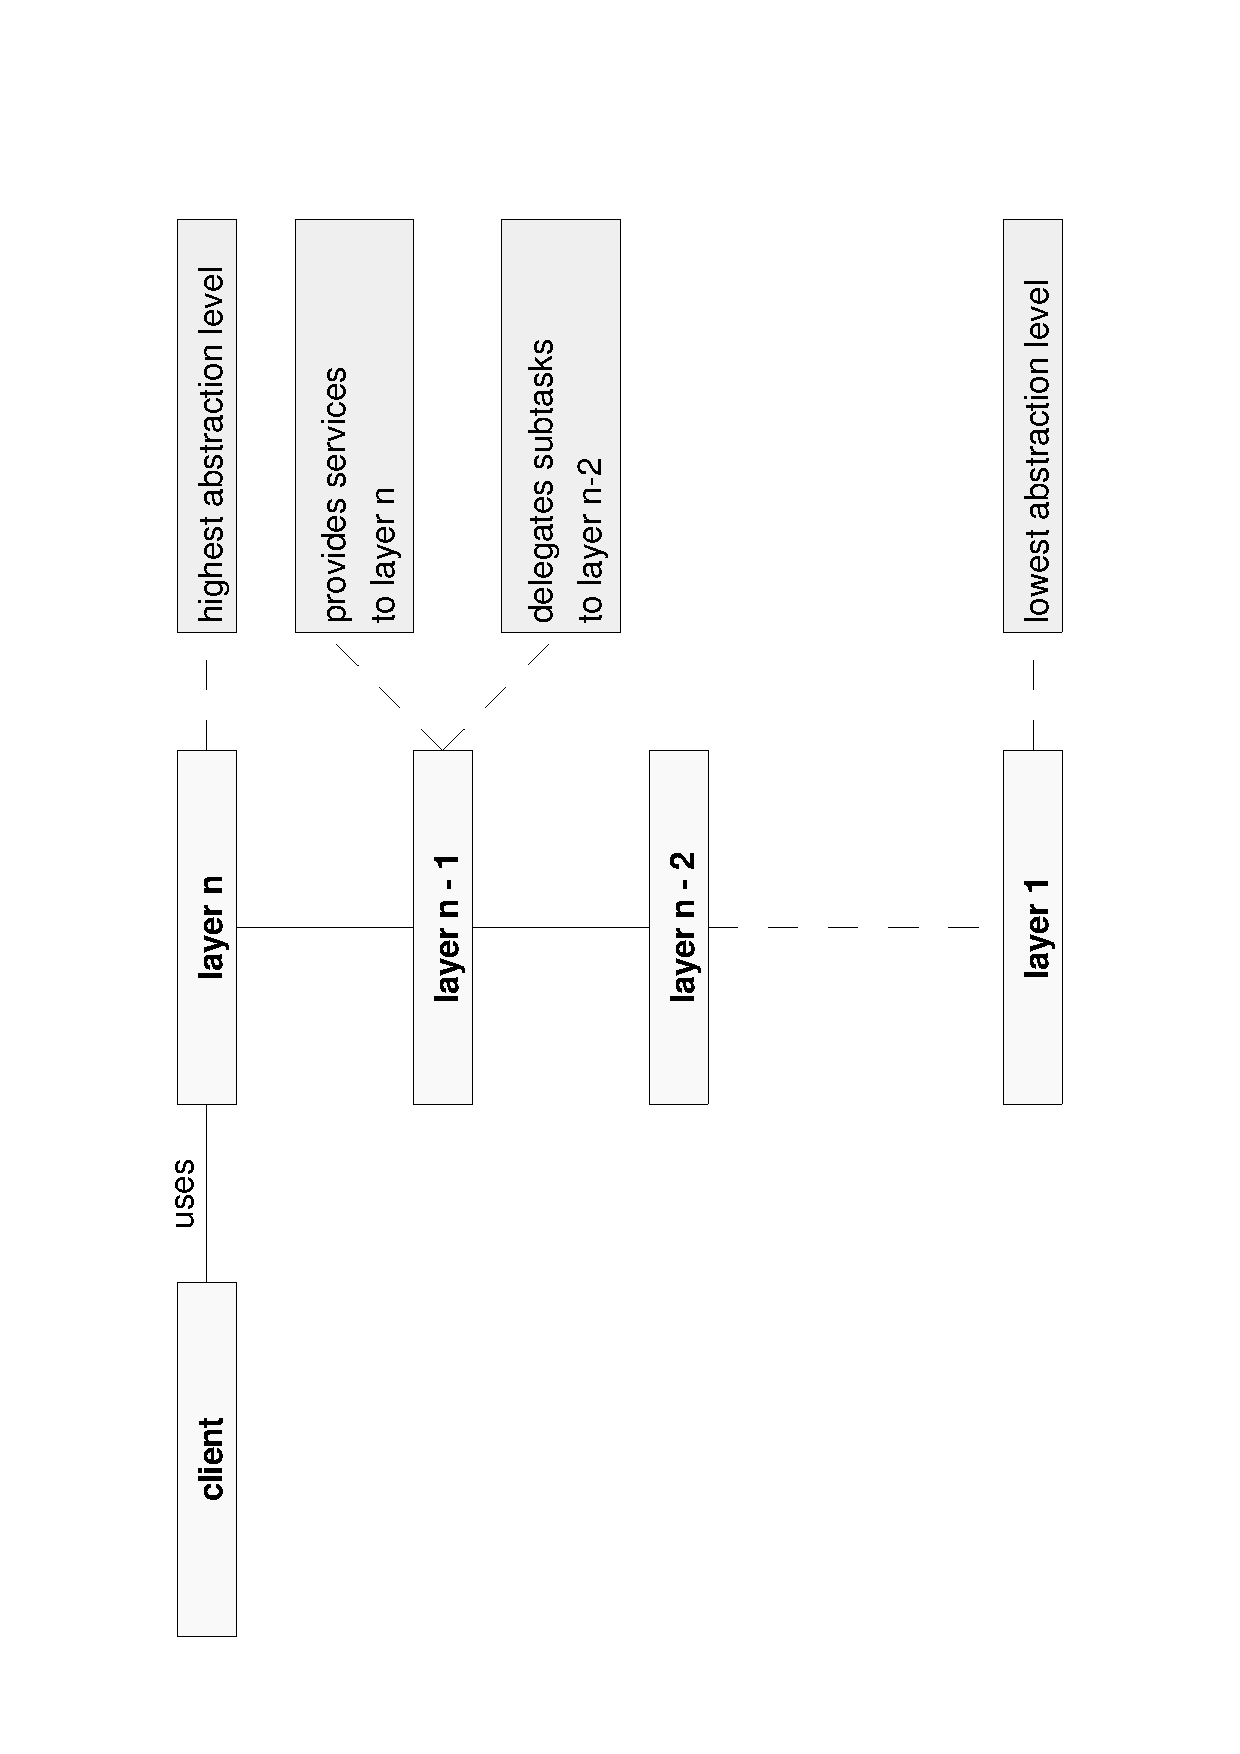
\includegraphics[scale=0.3,angle=-90]{graphic/layers.pdf}
        \caption{Layers Pattern}
        \label{layers_figure}
    \end{center}
\end{figure}

One variant of this pattern, mentioned by Buschmann \cite{buschmann}, is the
\emph{Relaxed-Layered-System}. It permits a layer to not only use the services
of its direct base layer, but also of yet lower-situated layers. The base layer,
in this case, is called \emph{transparent}.

The ontology examples in chapter \ref{knowledge_schema_heading} are organised
according to the \emph{Layers} pattern. Their layers represent levels of
growing granularity.

%
% $RCSfile: data_mapper.tex,v $
%
% Copyright (c) 2004. Christian Heller. All rights reserved.
%
% No copying, altering, distribution or any other actions concerning this
% document, except after explicit permission by the author!
% At some later point in time, this document is planned to be put under
% the GNU FDL license. For now, _everything_ is _restricted_ by the author.
%
% http://www.cybop.net
% - Cybernetics Oriented Programming -
%
% http://www.resmedicinae.org
% - Information in Medicine -
%
% @author Christian Heller <christian.heller@tuxtax.de>
%

\paragraph{Data Mapper}
\label{data_mapper_heading}

Besides the \emph{Domain Logic}, standard three-tier architectures contain a
\emph{Data Source} layer which may for example represent a database. Both layers
need to exchange data. Modern systems use OOP methods to implement the domain
model. Database models, on the other hand, are often implemented as
\emph{Entity Relationship Model} (ERM).

In order to avoid close coupling and a mix-up of both layers, the introduction
of an additional \emph{Data Mapper} layer \cite{fowler2002} in between the two
others may be justified (figure \ref{datamapper_figure}). The most important
idea of this pattern is to abolish the interdependencies of domain- and
persistence model (database).

\begin{figure}[ht]
    \begin{center}
        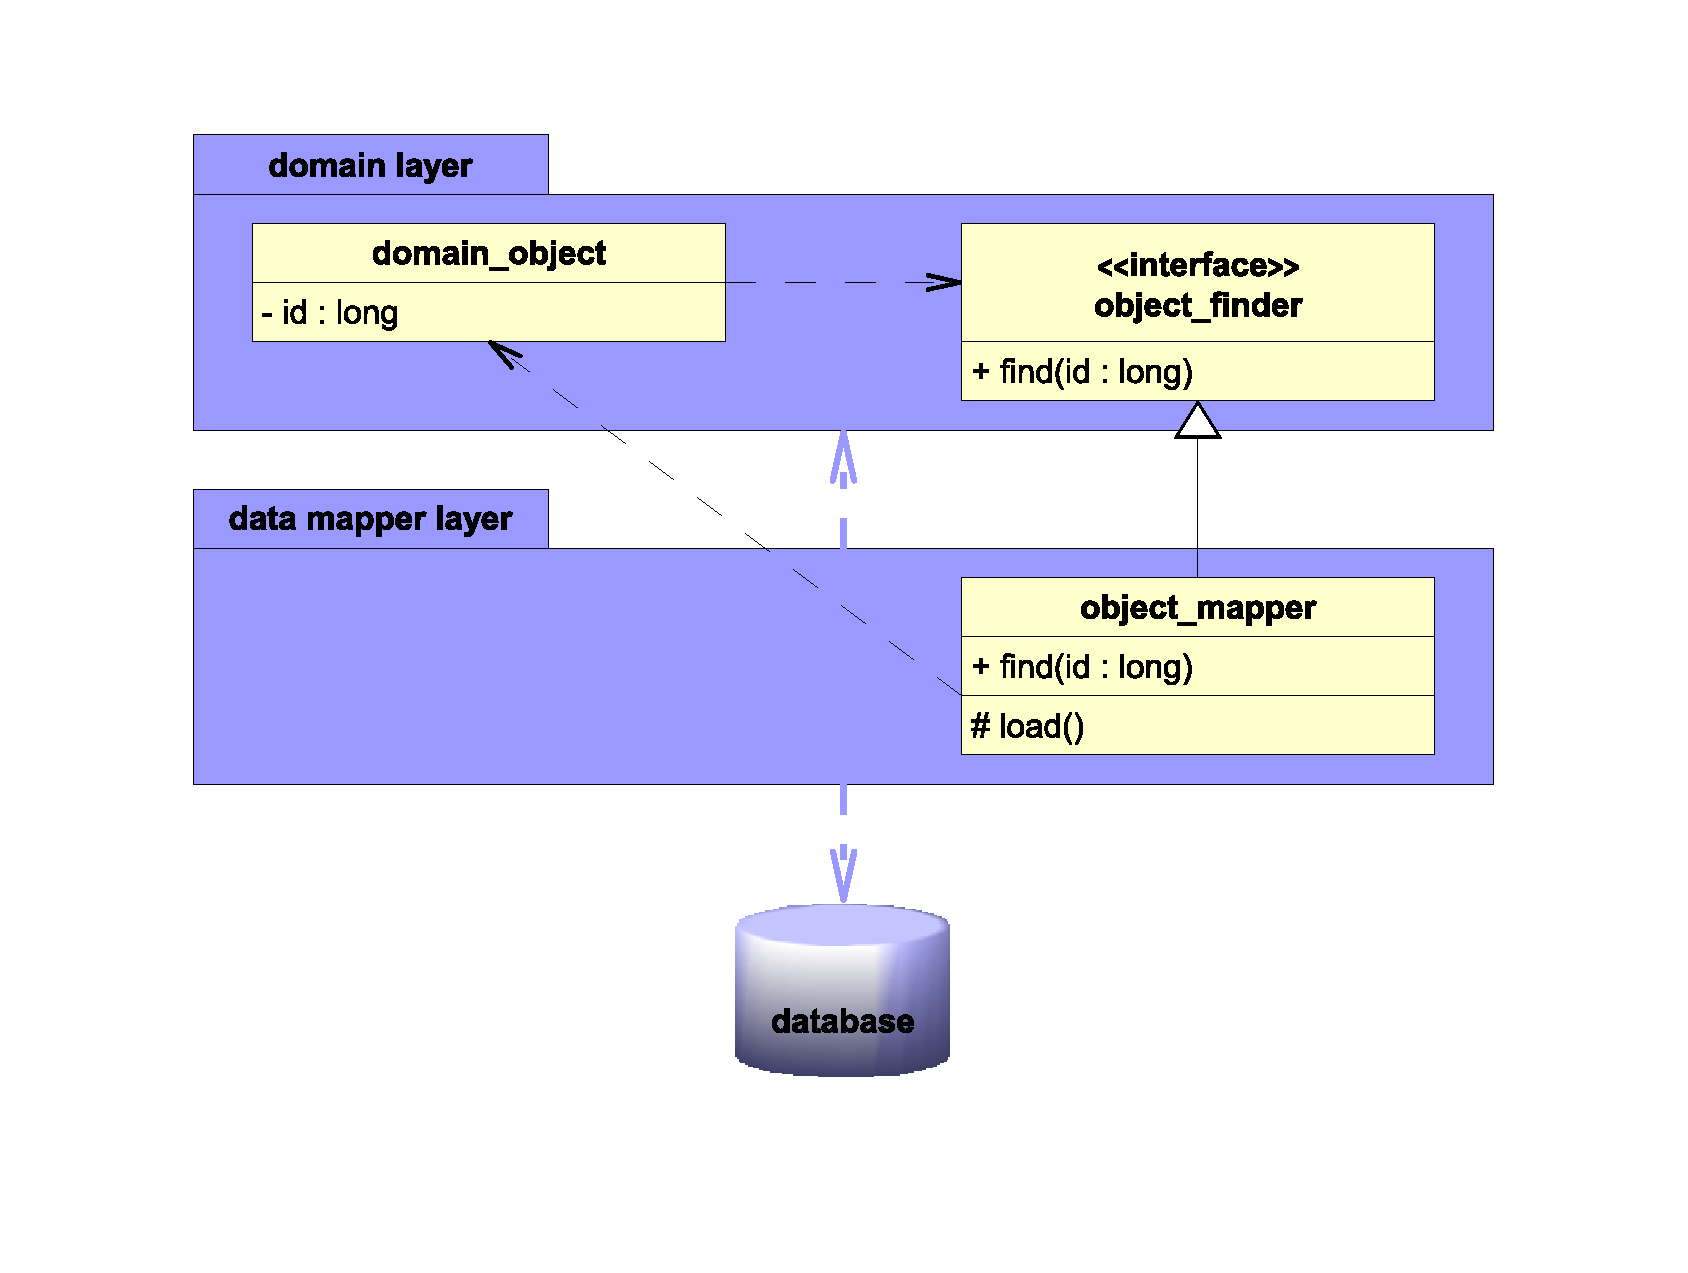
\includegraphics[scale=0.3]{vector/datamapper.eps}
        \caption{Data Mapper Pattern}
        \label{datamapper_figure}
    \end{center}
\end{figure}

The dashed arrows in figure \ref{datamapper_figure} indicate dependencies. The
data mapper layer knows the domain model- as well as the data source layer, via
\emph{unidirectional} relations. Its task is to \emph{translate} between the two,
in both directions. Domain model and data source know nothing from each other.

Each domain model class knows its appropriate interface (\emph{object\_finder})
but does not know the implementation of the same. That is, persistence- and
data retrieval mechanisms are hidden in front of the domain model. The
implementation (\emph{object\_mapper}) is part of the mapping package and also
implements all finder methods. It maps data of the received result sets to the
special attributes of the domain model objects.

The \emph{Mediator} pattern \cite{gamma1995} is similar to the \emph{Mapper}, in
that it is used to decouple different parts of a system. Fowler \cite{fowler2002}
writes: \textit{\ldots the objects that use a mediator are aware of it, even if
they aren't aware of each other; the objects that a mapper separates aren't even
aware of the mapper.}

Although the \emph{Data Mapper} pattern is very helpful at implementing OO
systems, two things are to be criticised:

Firstly, since the \emph{object\_finder} relies on functionality specific to the
retrieval of persistent data, it does actually belong into the data mapper layer
what, if done, would create bidirectional dependencies between the domain model-
and data mapper layer. But also with the \emph{object\_finder} remaining in the
domain model layer, dependencies are not purely unidirectional. It is true that
from an OO view, they are. Internally, however, a super class or interface
relates to its inheriting classes, so that it can call their methods to satisfy
the polymorphic behaviour.

Secondly, the layers do not truely build on each other. Taken a standard
architecture consisting of the following five -- instead of only three -- layers:

\begin{enumerate}
    \item Presentation
    \item Application Process
    \item Domain Model
    \item Data Mapper
    \item Data Source
\end{enumerate}

\ldots the application process does not only access the domain model layer, it
also has to manage (create and destroy) the objects of the data mapper layer.
In other words, it surpasses (disregards) the domain model layer when accessing
the data mapper layer directly.

%
% $RCSfile: data_transfer_object.tex,v $
%
% Copyright (C) 2002-2008. Christian Heller.
%
% Permission is granted to copy, distribute and/or modify this document
% under the terms of the GNU Free Documentation License, Version 1.1 or
% any later version published by the Free Software Foundation; with no
% Invariant Sections, with no Front-Cover Texts and with no Back-Cover
% Texts. A copy of the license is included in the section entitled
% "GNU Free Documentation License".
%
% http://www.cybop.net
% - Cybernetics Oriented Programming -
%
% http://www.resmedicinae.org
% - Information in Medicine -
%
% Version: $Revision: 1.1 $ $Date: 2008-08-19 20:41:06 $ $Author: christian $
% Authors: Christian Heller <christian.heller@tuxtax.de>
%

\subsubsection{Data Transfer Object}
\label{data_transfer_object_heading}
\index{Data Transfer Object Pattern}
\index{DTO}
\index{Assembler Object}
\index{Flat Data Structure}
\index{Translator Architecture}

\begin{figure}[ht]
    \begin{center}
       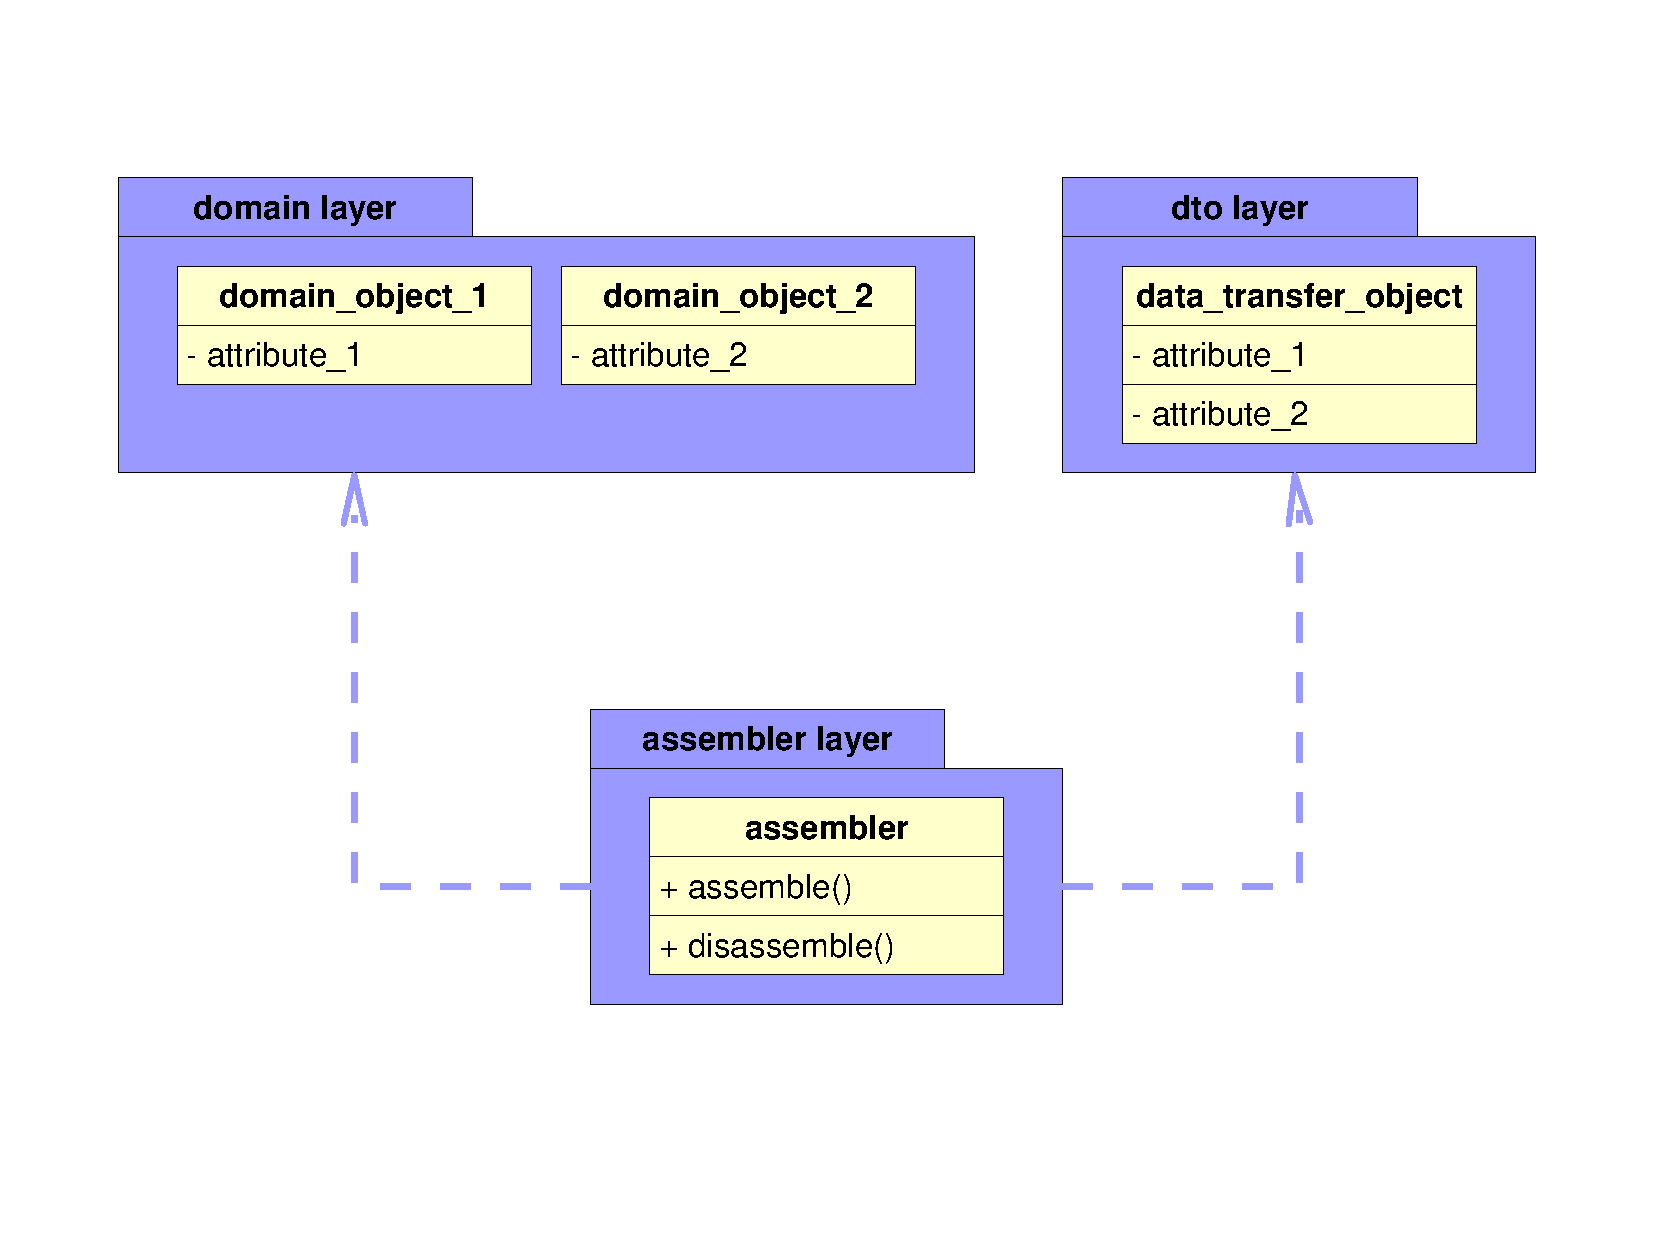
\includegraphics[scale=0.3,angle=-90]{graphic/dto.pdf}
       \caption{Data Transfer Object Pattern}
       \label{dto_figure}
    \end{center}
\end{figure}

It is a well-known fact that many small requests between two processes, and
even more between two hosts in a network need a lot of time. A local machine
with two processes has to permanently change the \emph{Program Context}; a
network has a lot of \emph{Transfers}. For each request, there is a necessity
of at least \emph{two} transfers -- the \emph{Question} of the client and the
\emph{Answer} of the server. Transfer methods are often expected to deliver
common data such as a Person's address, that is surname, first name, street,
zip-code, town and so on. These information is best retrieved by only
\emph{one} transfer call. That way, the client has to wait only once for a
server response and the server does not get too many single tasks. All address
data (in this example) would best be packaged together and sent back to the
client.

A scenario of that kind is exactly what the \emph{Data Transfer Object} pattern
\cite{fowler2002} proposes a solution for: A central \emph{Assembler} object
takes all common data of the server's domain model objects and assembles them
together into a special \emph{Data Transfer Object} (DTO), which is a flat data
structure (figure \ref{dto_figure}). The server will then send this DTO over
network to the client. On the client's side, a similar assembler takes the DTO,
finds out all received data and maps (disassembles) them to the client's domain
model. In that manner, a DTO is able to drastically improve the communication
performance.

Both, \emph{Data Mapper-} and DTO pattern translate one model into another. Due
to this similarity, chapter \ref{state_and_logic_heading} will try to merge
them into a common \emph{Translator} architecture.

%
% $RCSfile: model_view_controller.tex,v $
%
% Copyright (C) 2002-2008. Christian Heller.
%
% Permission is granted to copy, distribute and/or modify this document
% under the terms of the GNU Free Documentation License, Version 1.1 or
% any later version published by the Free Software Foundation; with no
% Invariant Sections, with no Front-Cover Texts and with no Back-Cover
% Texts. A copy of the license is included in the section entitled
% "GNU Free Documentation License".
%
% http://www.cybop.net
% - Cybernetics Oriented Programming -
%
% http://www.resmedicinae.org
% - Information in Medicine -
%
% Version: $Revision: 1.1 $ $Date: 2008-08-19 20:41:07 $ $Author: christian $
% Authors: Christian Heller <christian.heller@tuxtax.de>
%

\subsubsection{Model View Controller}
\label{model_view_controller_heading}
\index{Model View Controller Pattern}
\index{MVC}
\index{Graphical User Interface}
\index{GUI}
\index{Observer Pattern}
\index{Strategy Pattern}
\index{Wrapper Pattern}
\index{Composite Pattern}
\index{Java Foundation Classes}
\index{JFC}
\index{Microsoft Foundation Classes}
\index{MFC}
\index{Document View MVC Variant}
\index{Translator Architecture}

After having had a closer look at design patterns for persistence
(\emph{Data Mapper}) and communication (\emph{Data Transfer Object}), this
section considers the presentation layer of an application (figure
\ref{logical_figure}), which is often realised in form of a
\emph{Graphical User Interface} (GUI). Nowadays, the well-known
\emph{Model View Controller} (MVC) pattern \cite{buschmann, fowler2002} is used
by a majority of standard business applications. Its principle is to have the
\emph{Model} holding domain data, the \emph{View} accessing and displaying
these data and the \emph{Controller} providing the workflow of the application
by handling any action events happening on the view (figure \ref{mvc_figure}).
This separation eases the creation of applications with many synchronous views
on the same data. Internally, the MVC may consist of design patterns like:

\begin{figure}[ht]
    \begin{center}
        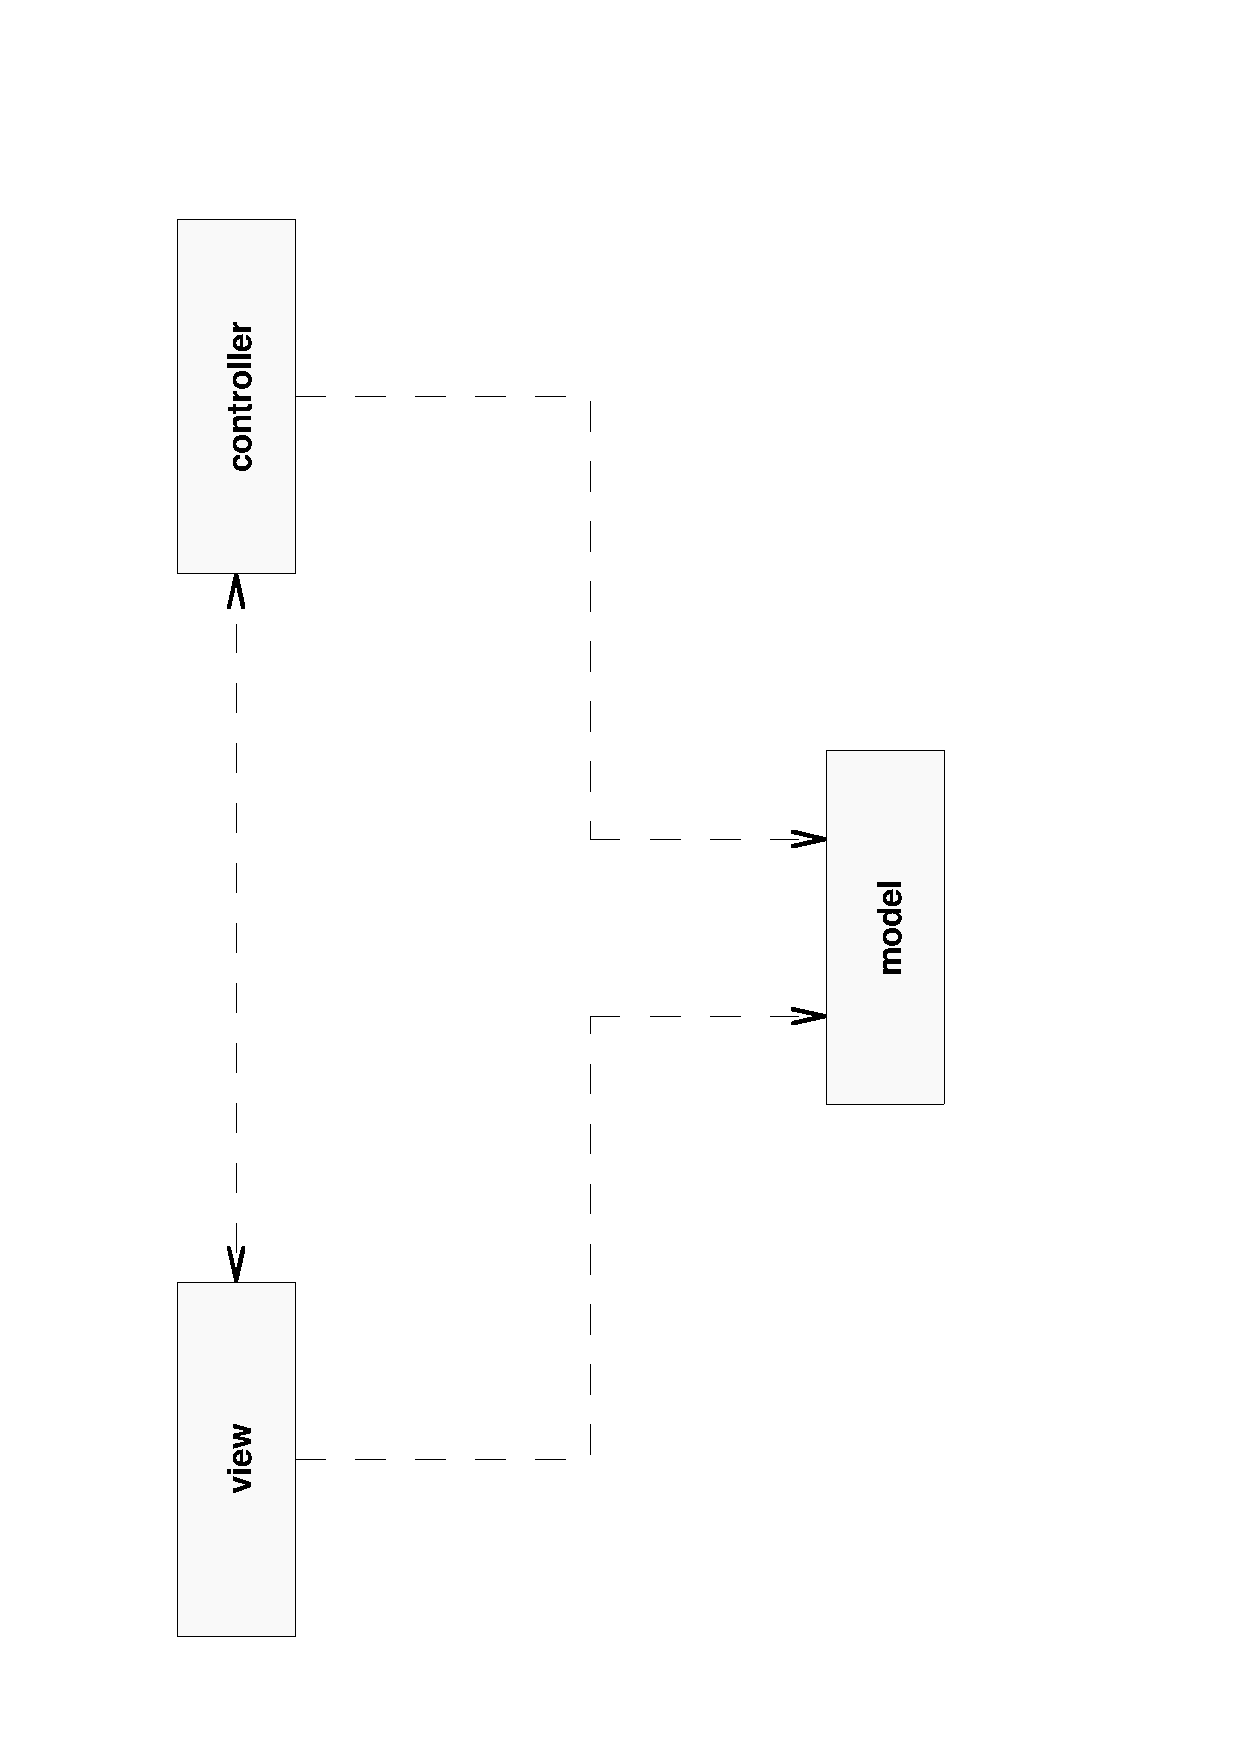
\includegraphics[scale=0.3,angle=-90]{graphic/mvc.pdf}
        \caption{Model View Controller Pattern}
        \label{mvc_figure}
    \end{center}
\end{figure}

\begin{itemize}
    \item[-] \emph{Observer} (section \ref{observer_heading}) which notifies
        the views about data model changes
    \item[-] \emph{Strategy} \cite{gamma1995} which encapsulates exchangeable
        functionality of the controller
    \item[-] \emph{Wrapper} (section \ref{wrapper_heading}) which delegates
        controller functionality to the \emph{Strategy}
    \item[-] \emph{Composite} (section \ref{composite_heading}) which equips
        graphical views with a hierarchical structure
\end{itemize}

Some MVC implementations like parts of the \emph{Java Foundation Classes} (JFC)
use a simplified version not separating controllers from their views. The
\emph{Microsoft Foundation Classes} (MFC) C++ library calls its implementation
\emph{Document-View}.

Besides the above-mentioned patterns \emph{Data Mapper} and DTO, MVC is the
third one getting merged into a common \emph{Translator} architecture, in
chapter \ref{state_and_logic_heading}.

%
% $RCSfile: hierarchical_model_view_controller.tex,v $
%
% Copyright (C) 2002-2008. Christian Heller.
%
% Permission is granted to copy, distribute and/or modify this document
% under the terms of the GNU Free Documentation License, Version 1.1 or
% any later version published by the Free Software Foundation; with no
% Invariant Sections, with no Front-Cover Texts and with no Back-Cover
% Texts. A copy of the license is included in the section entitled
% "GNU Free Documentation License".
%
% http://www.cybop.net
% - Cybernetics Oriented Programming -
%
% http://www.resmedicinae.org
% - Information in Medicine -
%
% Version: $Revision: 1.1 $ $Date: 2008-08-19 20:41:07 $ $Author: christian $
% Authors: Christian Heller <christian.heller@tuxtax.de>
%

\subsubsection{Hierarchical Model View Controller}
\label{hierarchical_model_view_controller_heading}
\index{Hierarchical Model View Controller Pattern}
\index{HMVC}
\index{Model View Controller Pattern}
\index{MVC}
\index{Composite Pattern}
\index{Layers Pattern}
\index{Chain of Responsibility Pattern}
\index{Presentation Layer}
\index{MVC Triad}
\index{Presentation Abstraction Control}
\index{PAC}
\index{PAC Agent}

There exist several extensions of the MVC pattern, one of them being the
\emph{Hierarchical Model View Controller} (HMVC) \cite{cai}. It combines the
patterns \emph{Composite} (section \ref{composite_heading}), \emph{Layers}
(section \ref{layers_heading}) and \emph{Chain of Responsibility} (section
\ref{chain_of_responsibility_heading}) into one conceptual architecture (figure
\ref{hmvc_figure}). This architecture divides the presentation layer into
hierarchical sections containing so-called \emph{MVC Triads}. The triads
conventionally consist of \emph{Model}, \emph{View} and \emph{Controller},
each. They communicate with each other by relating over their controller
object. Following the \emph{Layers} pattern, only neighbouring layers know from
each other.

\begin{figure}[ht]
    \begin{center}
        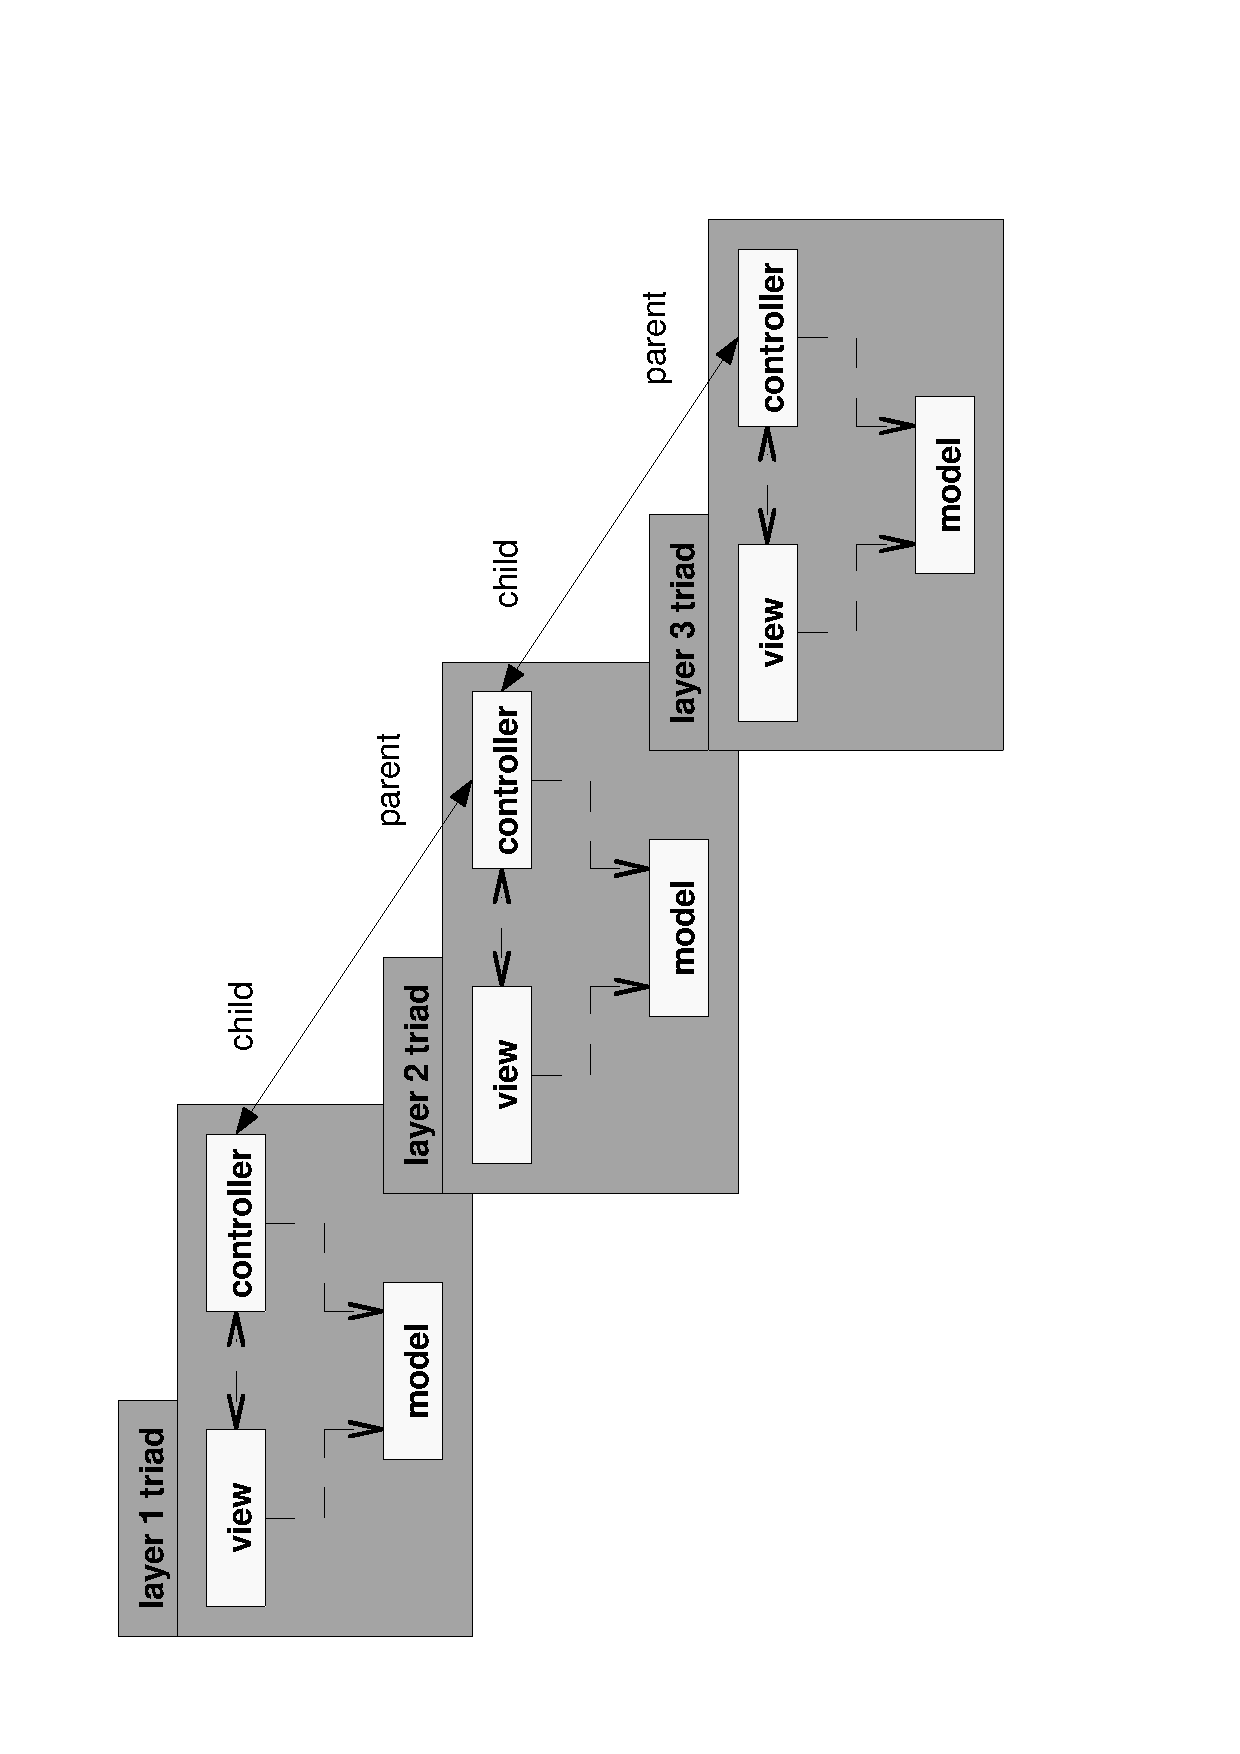
\includegraphics[scale=0.3,angle=-90]{graphic/hmvc.pdf}
        \caption{Hierarchical Model View Controller Pattern}
        \label{hmvc_figure}
    \end{center}
\end{figure}

As a practical example, the upper-most triad could represent a graphical
\emph{Dialogue} and the next lower one a \emph{Panel}. Being a container, too,
the panel could hold a third triad like for example a \emph{Button}. Events
occuring at the button are then normally processed by the corresponding
controller belonging to the button's triad. If, however, the button controller
cannot handle the event, that is forwarded along the chain of responsibility to
the controller of the higher-next layer. If also the panel controller does not
know how to handle the event, the final responsibility falls to the controller
of the dialogue's triad.

The HMVC is similar to the \emph{Presentation Abstraction Control} (PAC) pattern
\cite{buschmann}. A \emph{PAC Agent} is comparable to an \emph{HMVC Triad}.

Chapter \ref{knowledge_schema_heading} will apply the principle of
\emph{Hierarchy} not only to logic- (controller), but also to user interface-
(view), domain- and further models.

%
% $RCSfile: microkernel.tex,v $
%
% Copyright (c) 2004. Christian Heller. All rights reserved.
%
% No copying, altering, distribution or any other actions concerning this
% document, except after explicit permission by the author!
% At some later point in time, this document is planned to be put under
% the GNU FDL license. For now, _everything_ is _restricted_ by the author.
%
% http://www.cybop.net
% - Cybernetics Oriented Programming -
%
% http://www.resmedicinae.org
% - Information in Medicine -
%
% @author Christian Heller <christian.heller@tuxtax.de>
%

\paragraph{Microkernel}
\label{microkernel_heading}

The \emph{Microkernel} pattern \cite{buschmann} allows to keep a system flexible
and adaptable to changing requirements or new technologies. A minimal functional
\emph{Kernel} gets separated from extended functionality. The kernel may call
internal- or external servers (figure \ref{microkernel_figure}) to let them
solve special tasks which do not belong to its own core responsibility. Internal
servers are often called \emph{Daemons}.

\begin{figure}[ht]
    \begin{center}
        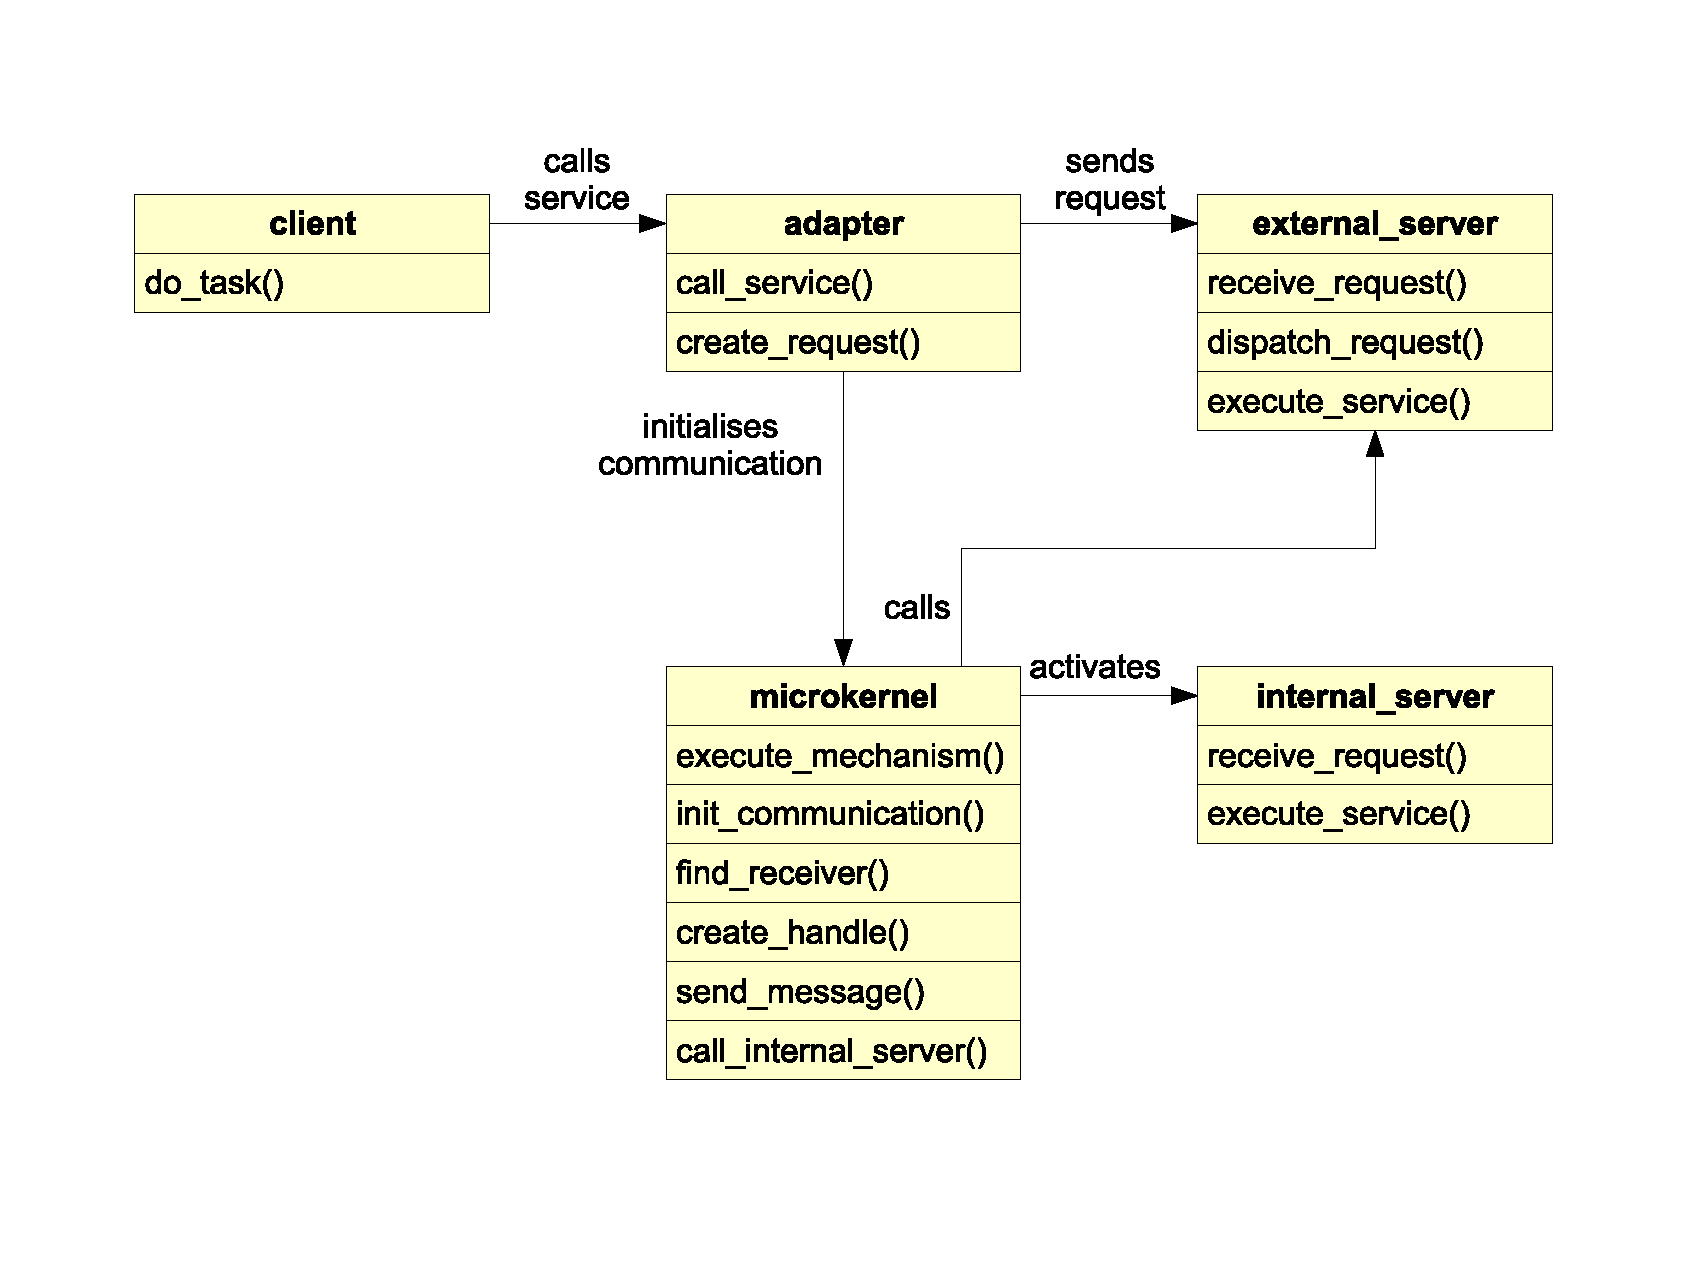
\includegraphics[scale=0.3]{vector/microkernel.eps}
        \caption{Microkernel Pattern}
        \label{microkernel_figure}
    \end{center}
\end{figure}

This pattern provides a \emph{Plug \& Play} environment and serves as base
architecture for many modern \emph{Operating Systems} (OS). Andrew S. Tanenbaum
recommends its use as well \cite{tanenbaum2001}.

%
% $RCSfile: broker.tex,v $
%
% Copyright (C) 2002-2008. Christian Heller.
%
% Permission is granted to copy, distribute and/or modify this document
% under the terms of the GNU Free Documentation License, Version 1.1 or
% any later version published by the Free Software Foundation; with no
% Invariant Sections, with no Front-Cover Texts and with no Back-Cover
% Texts. A copy of the license is included in the section entitled
% "GNU Free Documentation License".
%
% http://www.cybop.net
% - Cybernetics Oriented Programming -
%
% http://www.resmedicinae.org
% - Information in Medicine -
%
% Version: $Revision: 1.1 $ $Date: 2008-08-19 20:41:05 $ $Author: christian $
% Authors: Christian Heller <christian.heller@tuxtax.de>
%

\subsubsection{Broker}
\label{broker_heading}
\index{Broker Pattern}
\index{Distributed Application}

The \emph{Broker} pattern \cite{buschmann} may support the creation of an IT
infrastructure for distributed applications. It connects decoupled components
which interact through remote service invocations (figure \ref{broker_figure}).
The broker is responsible for coordinating all communication, for forwarding
requests as well as for transmitting results and exceptions.

%
% CAUTION! This file actually contains a graphics, which was moved to
% the 'microkernel.tex' file, for better formatting results in the document.
%

Chapter \ref{cybernetics_oriented_interpreter_heading} introduces an
interpreter program being able to act as broker.

%
% $RCSfile: pipes_and_filters.tex,v $
%
% Copyright (C) 2002-2008. Christian Heller.
%
% Permission is granted to copy, distribute and/or modify this document
% under the terms of the GNU Free Documentation License, Version 1.1 or
% any later version published by the Free Software Foundation; with no
% Invariant Sections, with no Front-Cover Texts and with no Back-Cover
% Texts. A copy of the license is included in the section entitled
% "GNU Free Documentation License".
%
% http://www.cybop.net
% - Cybernetics Oriented Programming -
%
% http://www.resmedicinae.org
% - Information in Medicine -
%
% Version: $Revision: 1.1 $ $Date: 2008-08-19 20:41:08 $ $Author: christian $
% Authors: Christian Heller <christian.heller@tuxtax.de>
%

\subsubsection{Pipes and Filters}
\label{pipes_and_filters_heading}
\index{Pipes and Filters Pattern}
\index{Push Scenario for Data Forwarding}
\index{Pull Scenario for Data Forwarding}
\index{Mixed Push-Pull-Pipeline Scenario for Data Forwarding}
\index{Independent Loops Scenario for Data Forwarding}

Systems that process streams of data may make use of the \emph{Pipes and Filters}
pattern \cite{buschmann}. It encapsulates every processing step in an own
\emph{Filter} component and forwards the data through channels which are called
\emph{Pipeline} (figure \ref{pipesfilters_figure}). The data forwarding can
follow various scenarios:

\begin{figure}[ht]
    \begin{center}
        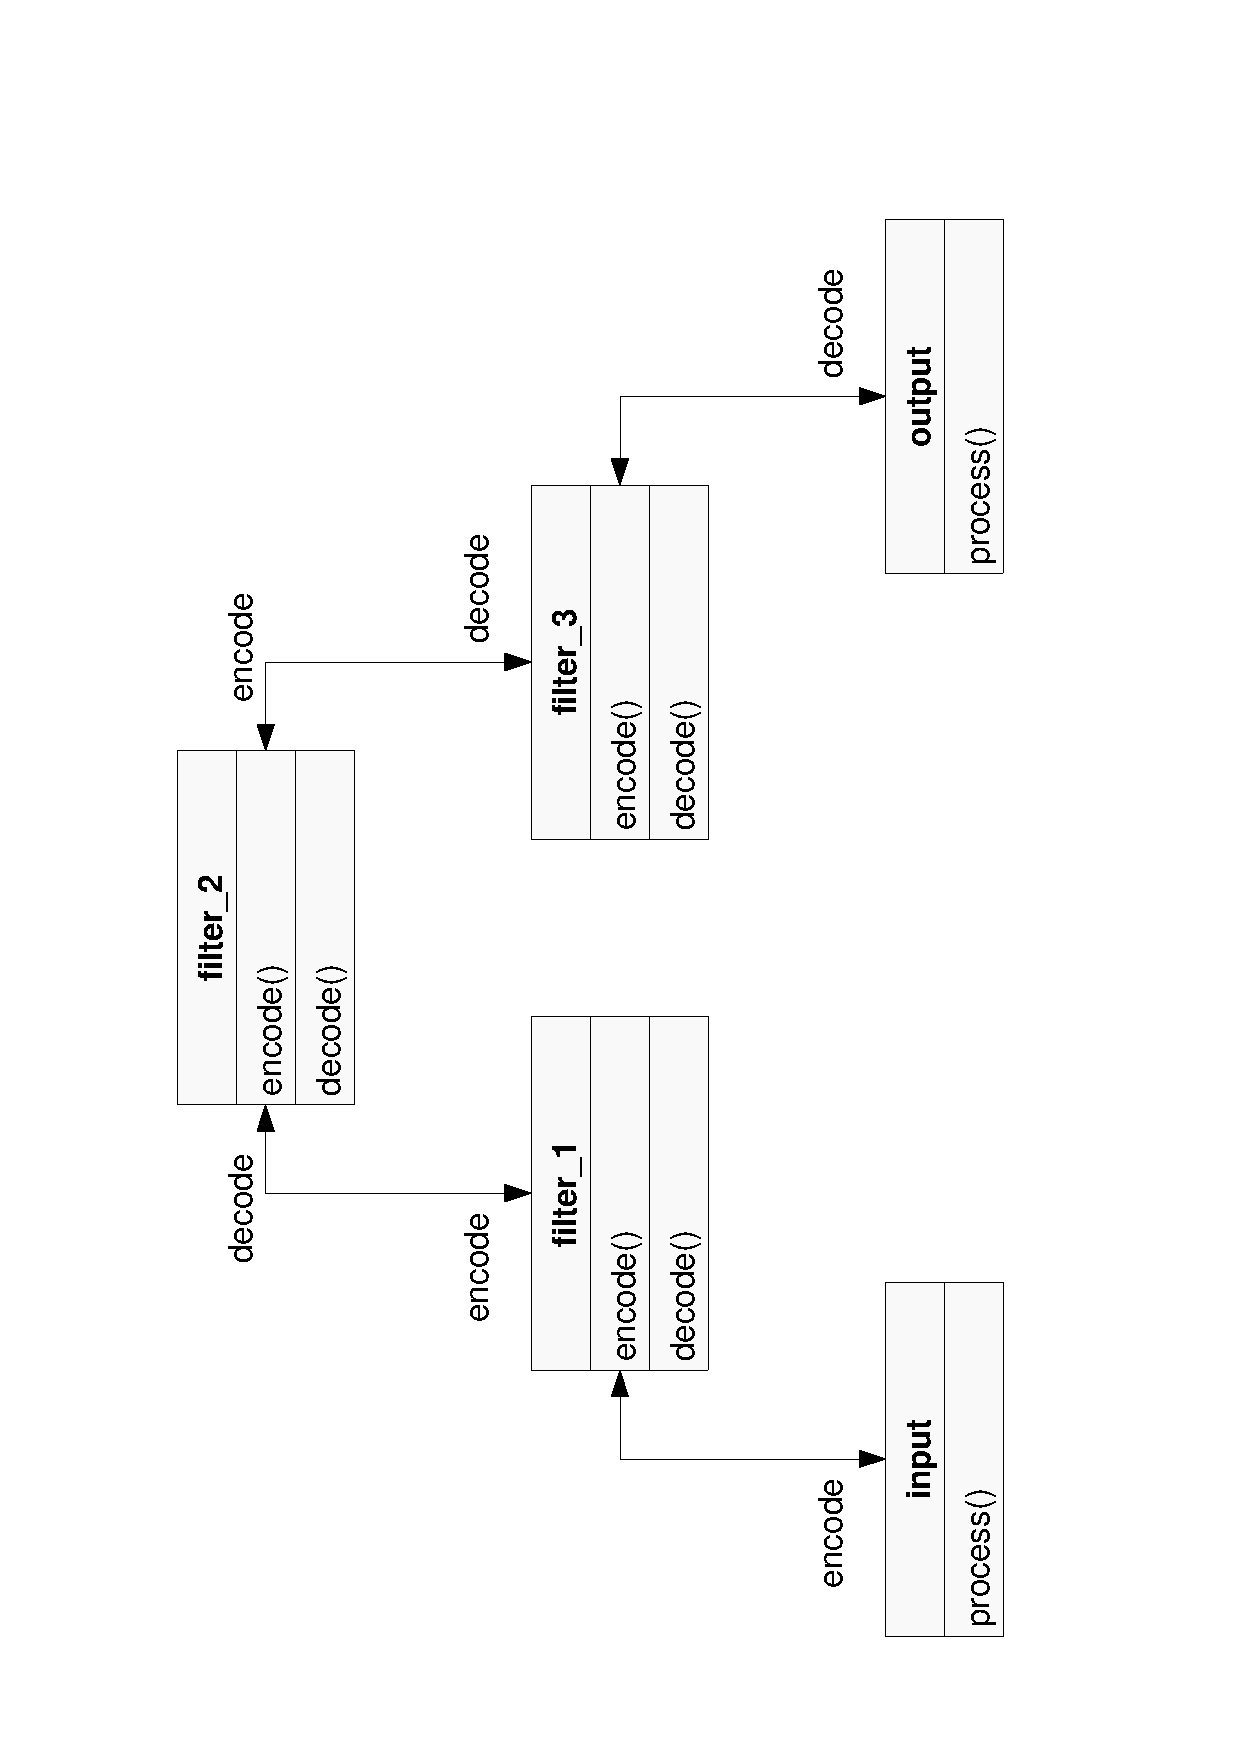
\includegraphics[scale=0.3,angle=-90]{graphic/pipesfilters.pdf}
        \caption{Pipes and Filters Pattern}
        \label{pipesfilters_figure}
    \end{center}
\end{figure}

\begin{itemize}
    \item[-] \emph{Push:} active filter pushes data to passive filter
    \item[-] \emph{Pull:} active filter pulls data from passive filter
    \item[-] \emph{Mixed Push-Pull-Pipeline:} all filters may push or pull data
    \item[-] \emph{Independent Loops:} all filters are active and access pipeline data
\end{itemize}

Families of related systems can be formed by changing the single filter
positions. Special communication filters are also used in the interpreter
program of chapter \ref{cybernetics_oriented_interpreter_heading}. Its filters
belong to neither of the above-listed forms of data forwarding, because they
are all passive, controlled from an outside entity which is not a filter
itself.

%
% $RCSfile: reflection.tex,v $
%
% Copyright (c) 2004. Christian Heller. All rights reserved.
%
% No copying, altering, distribution or any other actions concerning this
% document, except after explicit permission by the author!
% At some later point in time, this document is planned to be put under
% the GNU FDL license. For now, _everything_ is _restricted_ by the author.
%
% http://www.cybop.net
% - Cybernetics Oriented Programming -
%
% http://www.resmedicinae.org
% - Information in Medicine -
%
% @author Christian Heller <christian.heller@tuxtax.de>
%

\paragraph{Reflection}
\label{reflection_heading}

The \emph{Reflection} pattern \cite{buschmann} (also known under the synonyms
\emph{Open Implementation} or \emph{Meta-Level Architecture}) provides a
mechanism to change the structure and behaviour of a software system
\emph{dynamically}, that is at runtime, which is why that mechanism is sometimes
called \emph{Run Time Type Identification} (RTTI). A reflective system owns
information about itself and uses these to remain changeable and extensible.

\begin{figure}[ht]
    \begin{center}
        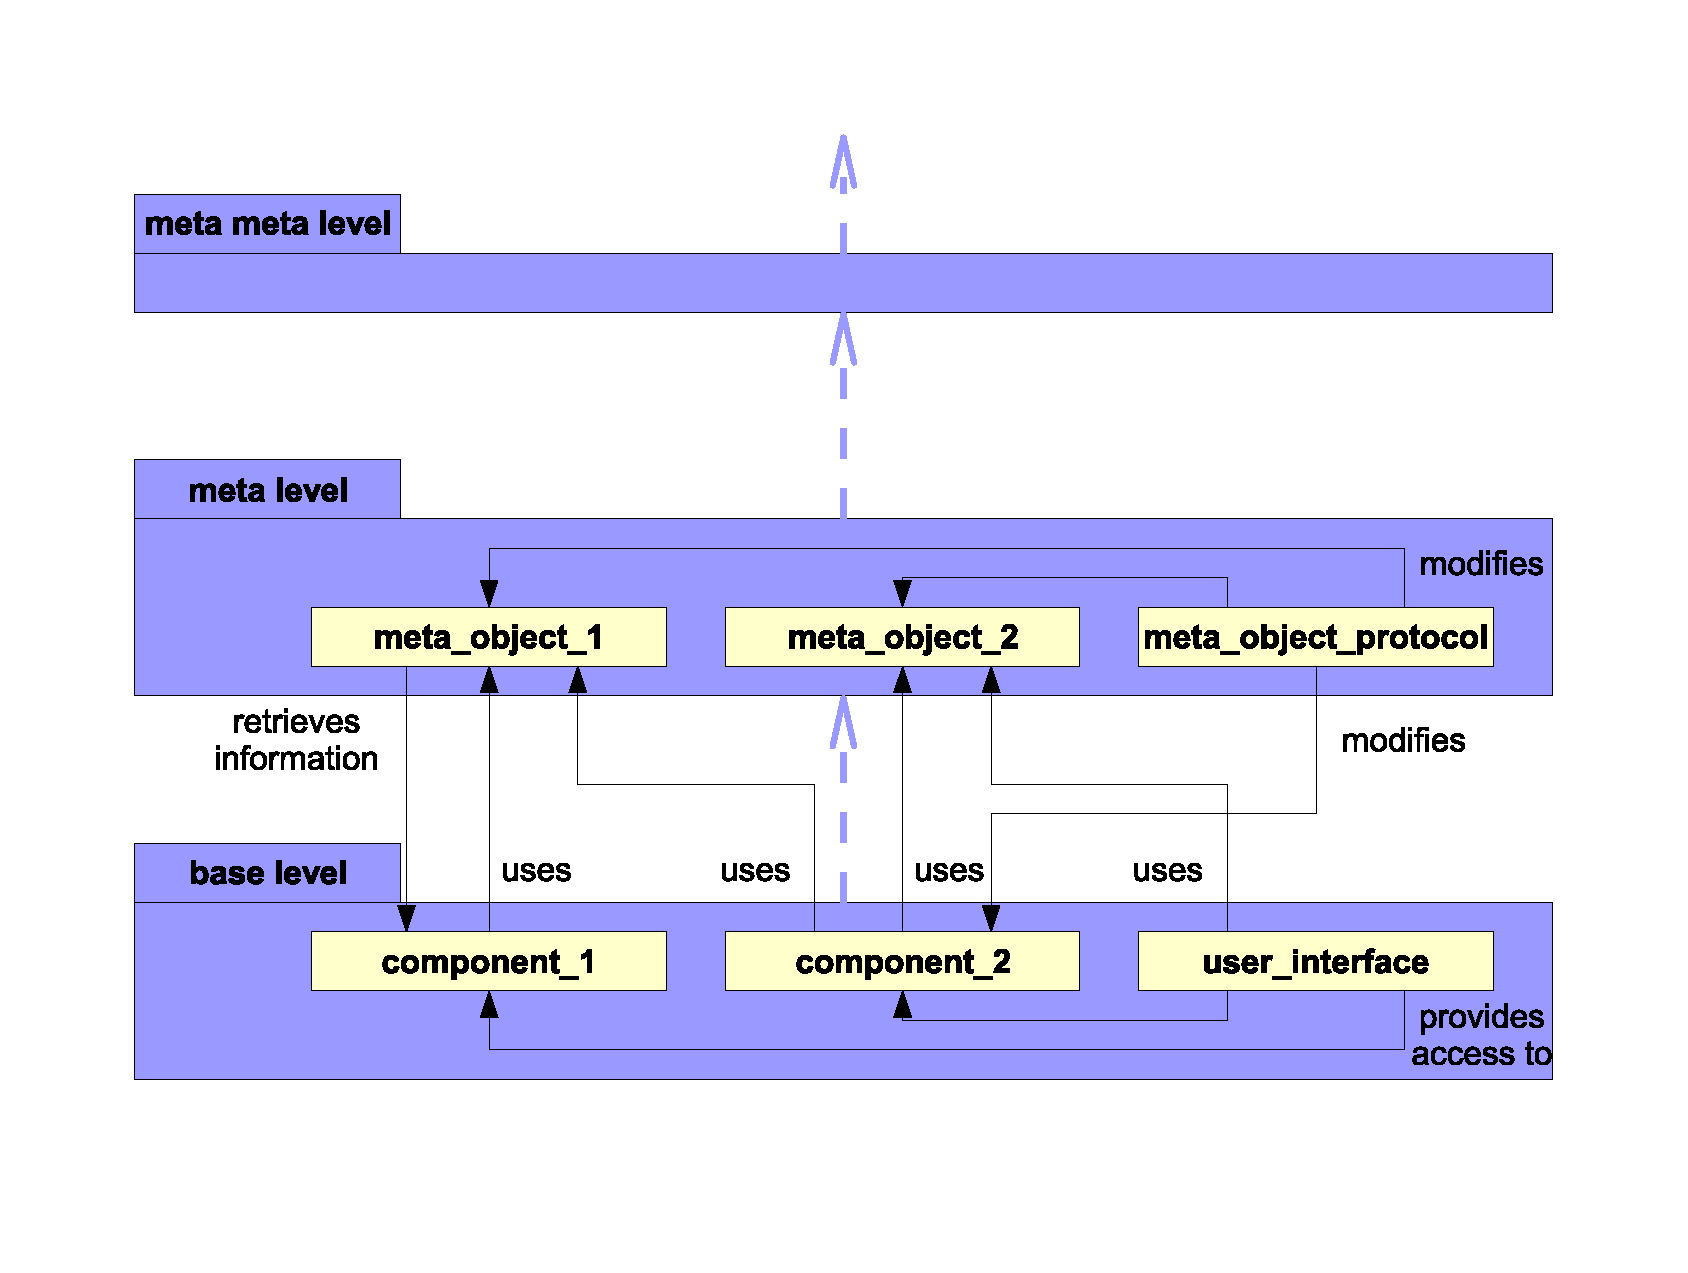
\includegraphics[scale=0.3]{vector/reflection.eps}
        \caption{Reflection Pattern}
        \label{reflection_figure}
    \end{center}
\end{figure}

Reflective information \emph{about} something is called \emph{Meta Information}.
Therefore, the level above the \emph{Base Level} in figure \ref{reflection_figure}
is labelled \emph{Meta Level}. The base level depends on the meta level, so that
changes in the meta level will also affect the base level. All manipulation of
meta objects happens through an interface called \emph{Meta Object Protocol}
(MOP), which is responsible for checking the correctness of- and for performing
a change. If a further level holds information about the meta level, then that
additional level is called \emph{Meta Meta Level}, and so forth.

Many examples of meta level architectures exist. In his book
\emph{Analysis Patterns} \cite{fowler1997}, Fowler uses them extensively.
He talks of \emph{Knowledge Level} (instead of meta level) and
\emph{Operational Level} (instead of base level). Elements of the
\emph{Unified Modeling Language} (UML) are defined in an own meta model
\cite{uml}. And the principles of reflection are also supported by several
programming languages, such as \emph{Smalltalk} \cite{smalltalk} and
\emph{Java} \cite{java}.

Classes (types) in a system have a static structure, as defined by the developer
at design time. Normally, most classes belong to the base level containing the
application logic. As written before, one way to change the structure and
behaviour of classes at runtime is to introduce a meta level providing type
information, in other words functionality that \emph{all} application classes
need. This helps avoid redundant implementations of the same functionality.

Looking closer at functionality, it turns out that some basic features like
persistence and communication occur repeatedly in almost all systems, while
other parts are specific to one concrete application. Traditionally, the
application classes in the base level have to cope with general system
functionality although that is not in their original interest. It therefore
seems logical to try to divide application- and system functionality, and to put
the latter into a meta level.


%
% $RCSfile: design.tex,v $
%
% Copyright (C) 2002-2008. Christian Heller.
%
% Permission is granted to copy, distribute and/or modify this document
% under the terms of the GNU Free Documentation License, Version 1.1 or
% any later version published by the Free Software Foundation; with no
% Invariant Sections, with no Front-Cover Texts and with no Back-Cover
% Texts. A copy of the license is included in the section entitled
% "GNU Free Documentation License".
%
% http://www.cybop.net
% - Cybernetics Oriented Programming -
%
% http://www.resmedicinae.org
% - Information in Medicine -
%
% Version: $Revision: 1.1 $ $Date: 2008-08-19 20:41:06 $ $Author: christian $
% Authors: Christian Heller <christian.heller@tuxtax.de>
%

\subsection{Design}
\label{design_heading}
\index{Design Pattern}

Gamma et al. \cite{gamma1995} define a design pattern as: \textit{description of
collaborating objects and classes which are taylored to solve a general design
problem in a special context.} Mostly, patterns are in relation to each other.
They can be combined to master more complex tasks.

%
% $RCSfile: command.tex,v $
%
% Copyright (c) 2004. Christian Heller. All rights reserved.
%
% No copying, altering, distribution or any other actions concerning this
% document, except after explicit permission by the author!
% At some later point in time, this document is planned to be put under
% the GNU FDL license. For now, _everything_ is _restricted_ by the author.
%
% http://www.cybop.net
% - Cybernetics Oriented Programming -
%
% http://www.resmedicinae.org
% - Information in Medicine -
%
% @author Christian Heller <christian.heller@tuxtax.de>
%

\paragraph{Command}
\label{command_heading}

The \emph{Command} pattern \cite{gamma1995}, also known as \emph{Action} or
\emph{Transaction}, sometimes also \emph{Signal}, encapsulates a command in
form of an object. That way, operations can get parameterised; they can be put
in a queue, be made undone or traced in a log book. Figure \ref{command_figure}
shows the structure of the pattern.

\begin{figure}[ht]
    \begin{center}
        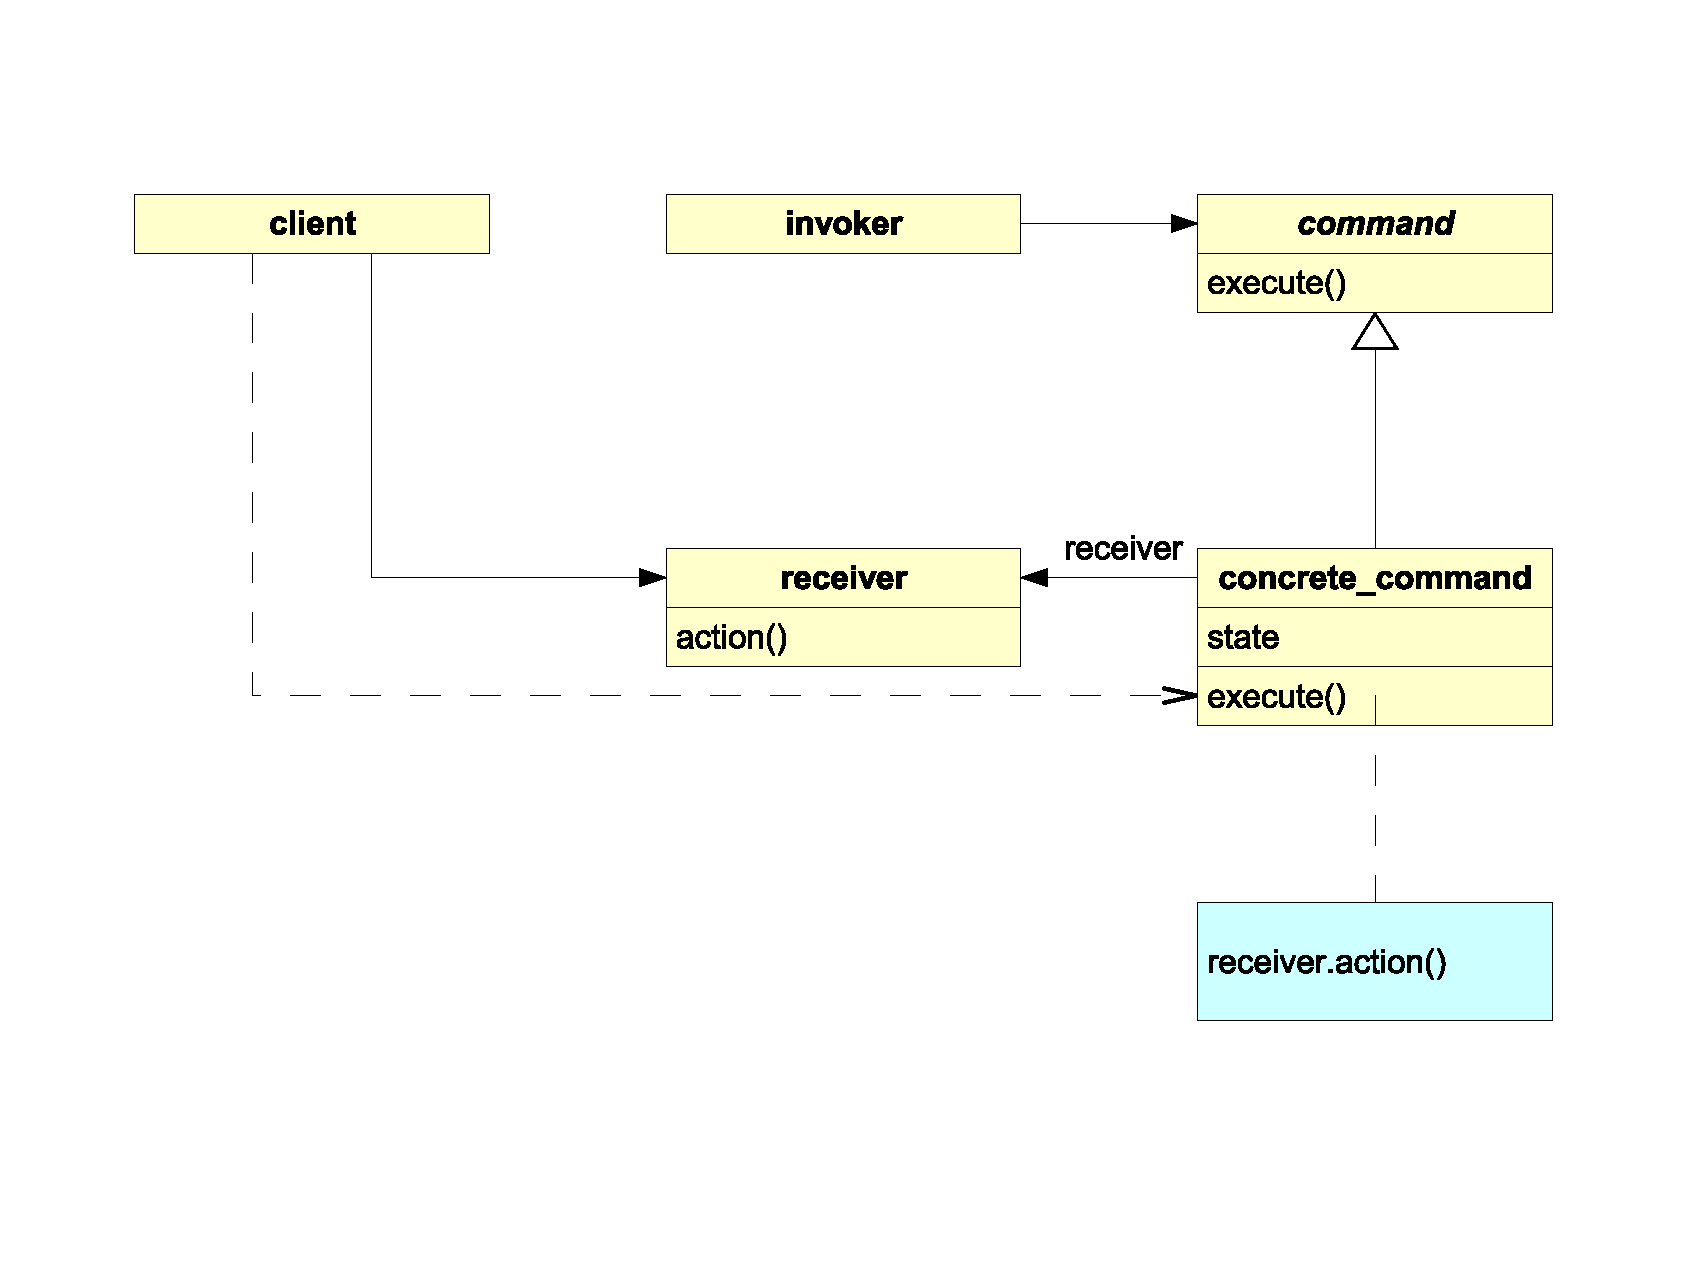
\includegraphics[scale=0.3]{vector/command.eps}
        \caption{Command Pattern}
        \label{command_figure}
    \end{center}
\end{figure}

%
% $RCSfile: wrapper.tex,v $
%
% Copyright (C) 2002-2008. Christian Heller.
%
% Permission is granted to copy, distribute and/or modify this document
% under the terms of the GNU Free Documentation License, Version 1.1 or
% any later version published by the Free Software Foundation; with no
% Invariant Sections, with no Front-Cover Texts and with no Back-Cover
% Texts. A copy of the license is included in the section entitled
% "GNU Free Documentation License".
%
% http://www.cybop.net
% - Cybernetics Oriented Programming -
%
% http://www.resmedicinae.org
% - Information in Medicine -
%
% Version: $Revision: 1.1 $ $Date: 2008-08-19 20:41:09 $ $Author: christian $
% Authors: Christian Heller <christian.heller@tuxtax.de>
%

\subsubsection{Wrapper}
\label{wrapper_heading}
\index{Wrapper Pattern}
\index{Adapter Pattern}
\index{Delegation Pattern}

The \emph{Wrapper} pattern \cite{gamma1995} allows otherwise incompatible
classes to work together. It can be seen as skin object enclosing (wrapping) an
inner core object, to which it provides access. In other words: It adapts the
interface of a class which is why Gamma et al. call the pattern \emph{Adapter}.
As can be seen in figure \ref{wrapper_figure}, this pattern makes heavy use of
\emph{Delegation}, where the \emph{Delegator} is the adapter (or wrapper) and
the \emph{Delegatee} is the class being adapted \cite{portland}.

\begin{figure}[ht]
    \begin{center}
        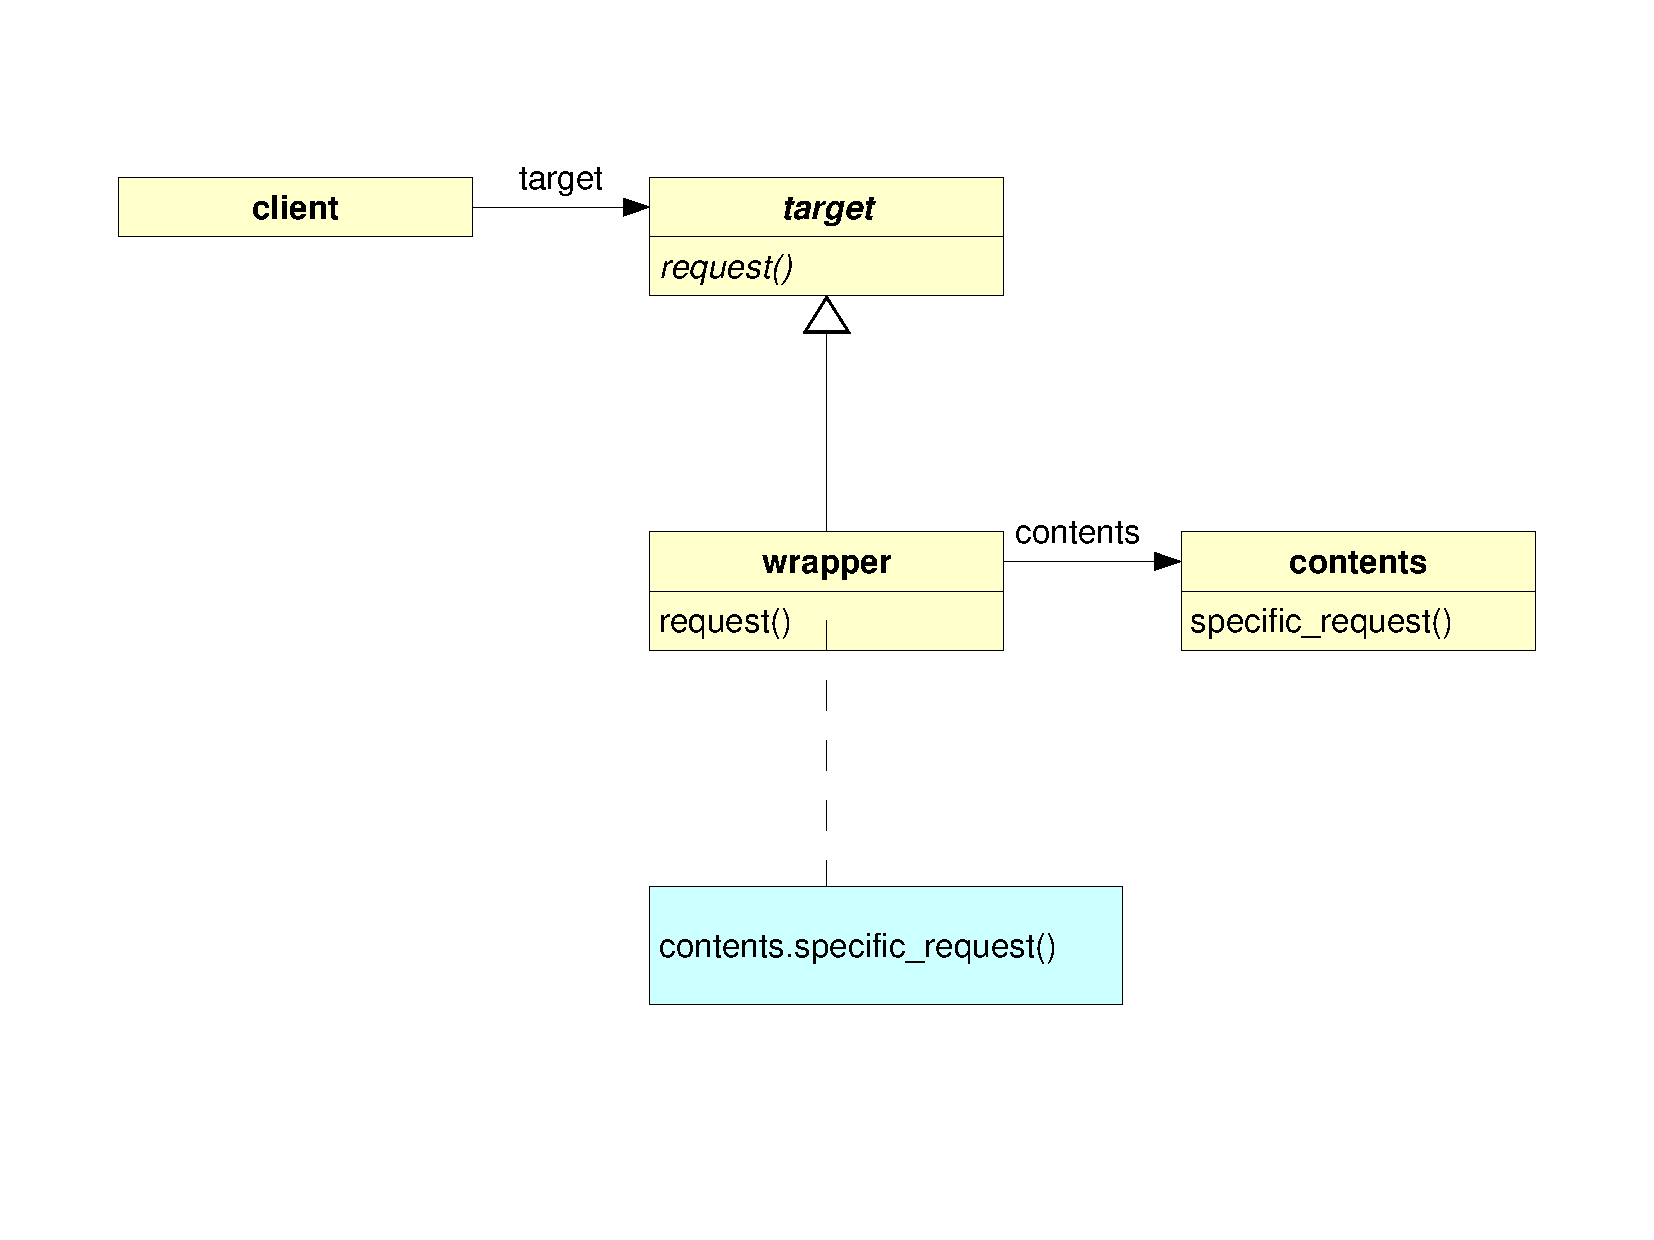
\includegraphics[scale=0.3,angle=-90]{graphic/wrapper.pdf}
        \caption{Wrapper Pattern}
        \label{wrapper_figure}
    \end{center}
\end{figure}

Knowledge templates created in the language described in chapter
\ref{cybernetics_oriented_language_heading} wrap the more fine-granular
templates they consist of.

%
% $RCSfile: whole_part.tex,v $
%
% Copyright (c) 2004. Christian Heller. All rights reserved.
%
% No copying, altering, distribution or any other actions concerning this
% document, except after explicit permission by the author!
% At some later point in time, this document is planned to be put under
% the GNU FDL license. For now, _everything_ is _restricted_ by the author.
%
% http://www.cybop.net
% - Cybernetics Oriented Programming -
%
% http://www.resmedicinae.org
% - Information in Medicine -
%
% @author Christian Heller <christian.heller@tuxtax.de>
%

\paragraph{Whole Part}
\label{whole_part_heading}

Whenever many components form a semantic unit, they can be subsumed by the
\emph{Whole-Part} pattern \cite{buschmann}. It encapsulates single part objects
(figure \ref{wholepart_figure}) and controls their cooperation. Part objects
are not addressable directly.

Almost all software systems contain components or sub systems which could be
organized by help of this pattern. In some way, it is quite similar to the
previously introduced \emph{Wrapper}, only that not just one- but many objects
are wrapped.

\begin{figure}[ht]
    \begin{center}
        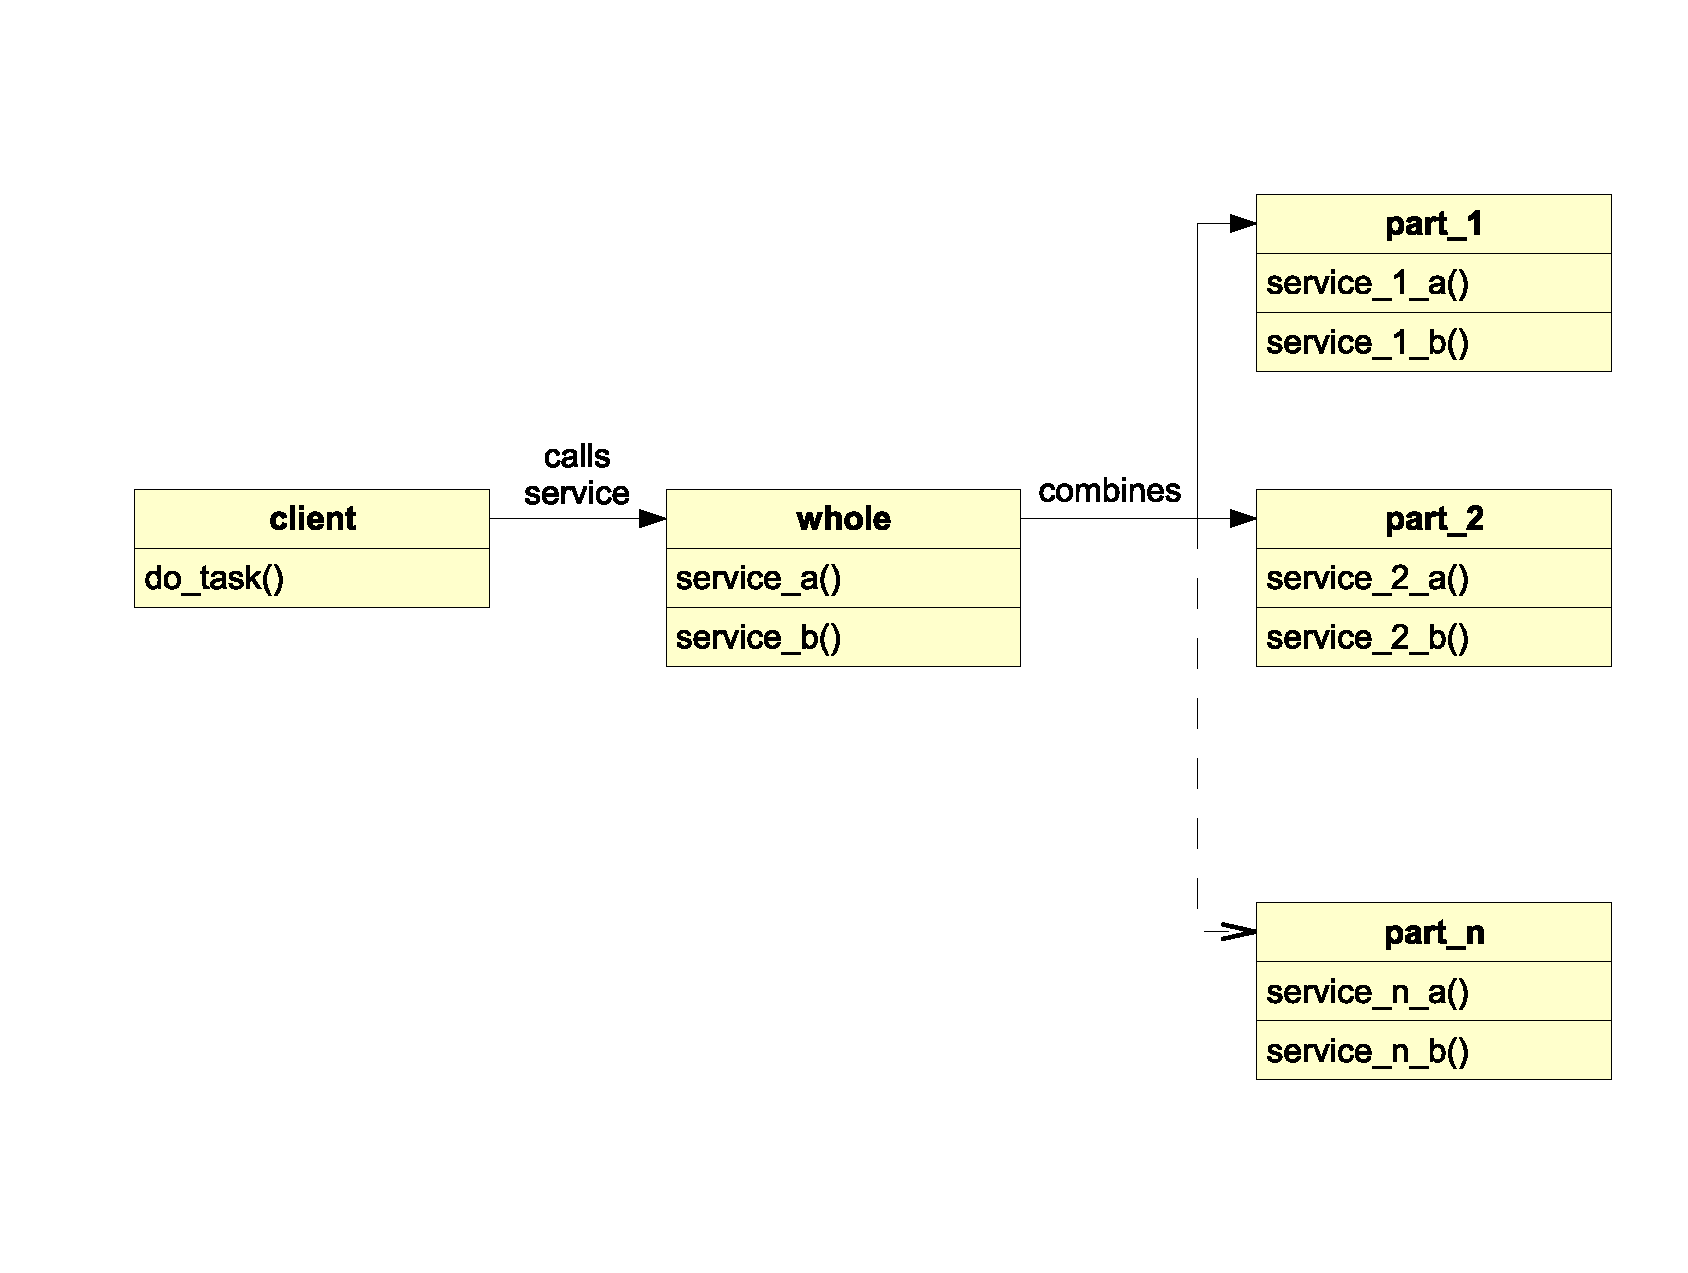
\includegraphics[scale=0.3]{vector/wholepart.eps}
        \caption{Whole-Part Pattern}
        \label{wholepart_figure}
    \end{center}
\end{figure}

%
% $RCSfile: composite.tex,v $
%
% Copyright (c) 2004. Christian Heller. All rights reserved.
%
% No copying, altering, distribution or any other actions concerning this
% document, except after explicit permission by the author!
% At some later point in time, this document is planned to be put under
% the GNU FDL license. For now, _everything_ is _restricted_ by the author.
%
% http://www.cybop.net
% - Cybernetics Oriented Programming -
%
% http://www.resmedicinae.org
% - Information in Medicine -
%
% @author Christian Heller <christian.heller@tuxtax.de>
%

\paragraph{Composite}
\label{composite_heading}

A hierarchical object structure, also called \emph{Directed Acyclical Graph}
(DAG) or \emph{Tree}, can be represented by a combination of classes called
\emph{Composite} pattern \cite{gamma1995}. It describes a \emph{Component} that
may consist of \emph{Children} (figure \ref{composite_figure}), which makes it
comparable to the \emph{Whole-Part} pattern. The difference is that the
\emph{Composite} is a more generalized version, with a dynamically extensible
number of child (part) objects.

The \emph{Composite} is a pattern based on \emph{Recursion}, which is one of
the most commonly used programming techniques at all. The pattern's split into
\emph{Leaf-} and \emph{Composite} sub classes helps distinguish primitive- from
container objects. A composite tree node holds objects of type \emph{Component}.

\begin{figure}[ht]
    \begin{center}
        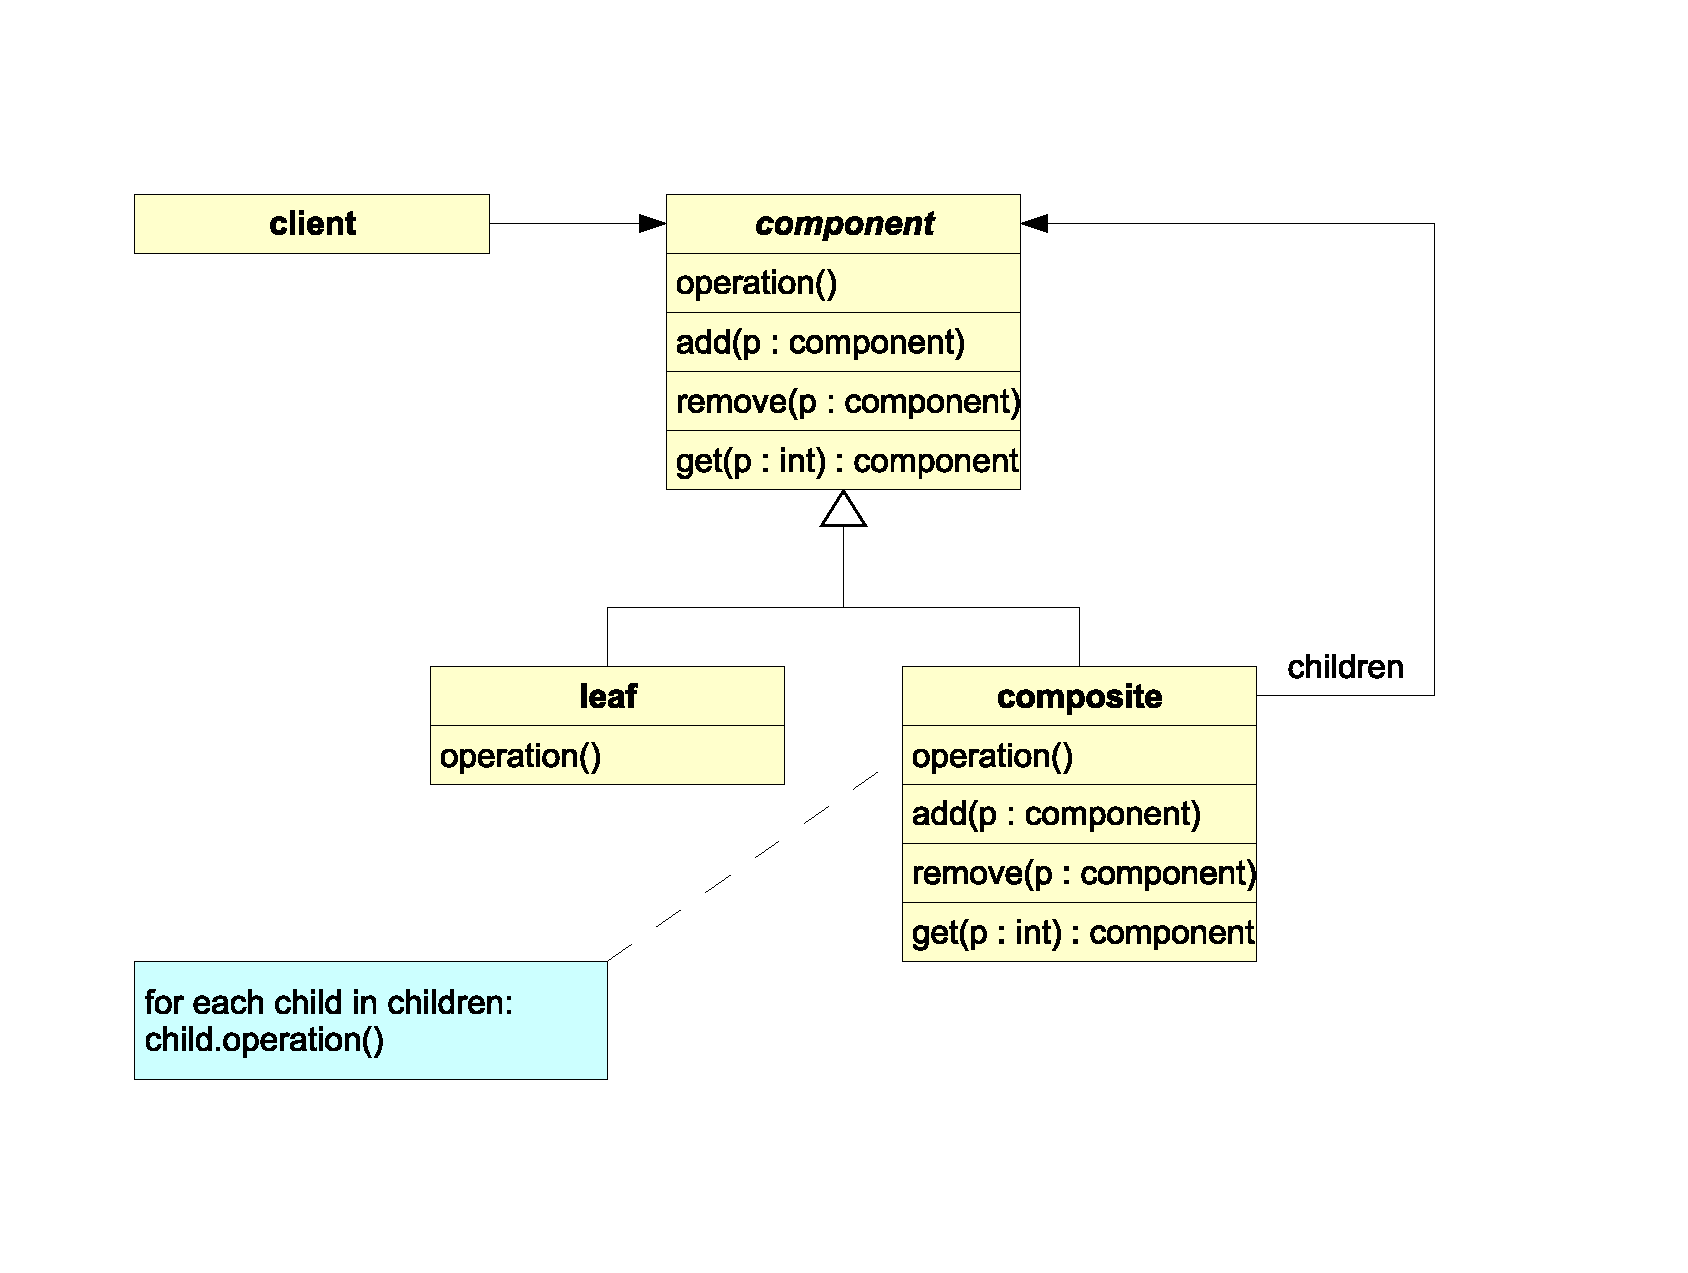
\includegraphics[scale=0.3]{vector/composite.eps}
        \caption{Composite Pattern}
        \label{composite_figure}
    \end{center}
\end{figure}

%
% $RCSfile: chain_of_responsibility.tex,v $
%
% Copyright (c) 2004. Christian Heller. All rights reserved.
%
% No copying, altering, distribution or any other actions concerning this
% document, except after explicit permission by the author!
% At some later point in time, this document is planned to be put under
% the GNU FDL license. For now, _everything_ is _restricted_ by the author.
%
% http://www.cybop.net
% - Cybernetics Oriented Programming -
%
% http://www.resmedicinae.org
% - Information in Medicine -
%
% @author Christian Heller <christian.heller@tuxtax.de>
%

\paragraph{Chain of Responsibility}
\label{chain_of_responsibility_heading}

The \emph{Chain of Responsibility} pattern \cite{gamma1995} is similar to the
\emph{Composite}, in that it represents a recursive structure as well. Objects
destined to solve a task are linked with a corresponding \emph{Successor}
(figure \ref{chain_figure}), such forming a chain. If an object is not able to
solve a task, that task is forwarded to the object's successor, along the chain.

\begin{figure}[ht]
    \begin{center}
        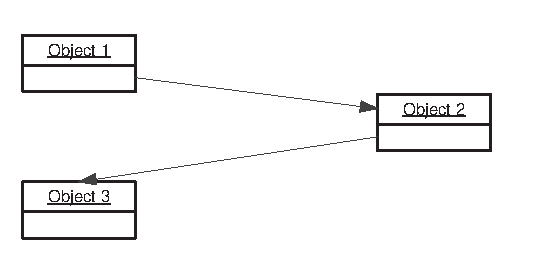
\includegraphics[scale=0.3]{vector/chain.eps}
        \caption{Chain of Responsibility Pattern}
        \label{chain_figure}
    \end{center}
\end{figure}

The pattern found wide application, for example in help systems, in event
handling frameworks or for exception handling. Its \emph{Handler} class is
known under synonyms like \emph{Event Handler}, \emph{Bureaucrat} or
\emph{Responder}.

Frequently, the pattern gets misused by delegating messages not only to children
but also to the parent of objects. The \emph{Hierarhical Model View Controller}
(HMVC) pattern is one example for this. It causes unfavourable bidirectional
dependencies (section \ref{bidirectional_dependency_heading}) and leads to
stronger coupling between the layers of a framework, because parent- and child
objects then reference each other.

%
% $RCSfile: observer.tex,v $
%
% Copyright (c) 2004. Christian Heller. All rights reserved.
%
% No copying, altering, distribution or any other actions concerning this
% document, except after explicit permission by the author!
% At some later point in time, this document is planned to be put under
% the GNU FDL license. For now, _everything_ is _restricted_ by the author.
%
% http://www.cybop.net
% - Cybernetics Oriented Programming -
%
% http://www.resmedicinae.org
% - Information in Medicine -
%
% @author Christian Heller <christian.heller@tuxtax.de>
%

\paragraph{Observer}
\label{observer_heading}

Another pattern that found wide application is the \emph{Observer} \cite{gamma1995},
an often-used synonym for which is \emph{Publisher-Subscriber}. It provides a
notification mechanism for all objects that registered as \emph{Observer} at a
\emph{Subject} in whose state changes they are interested, leading to an automatic
update of all dependent objects (figure \ref{observer_figure}).

\begin{figure}[ht]
    \begin{center}
        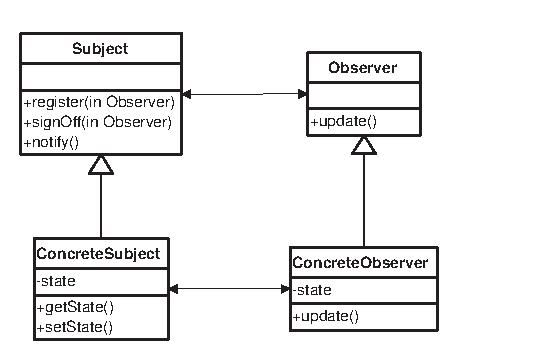
\includegraphics[scale=0.3]{vector/observer.eps}
        \caption{Observer Pattern}
        \label{observer_figure}
    \end{center}
\end{figure}

\begin{figure}[ht]
    \begin{center}
        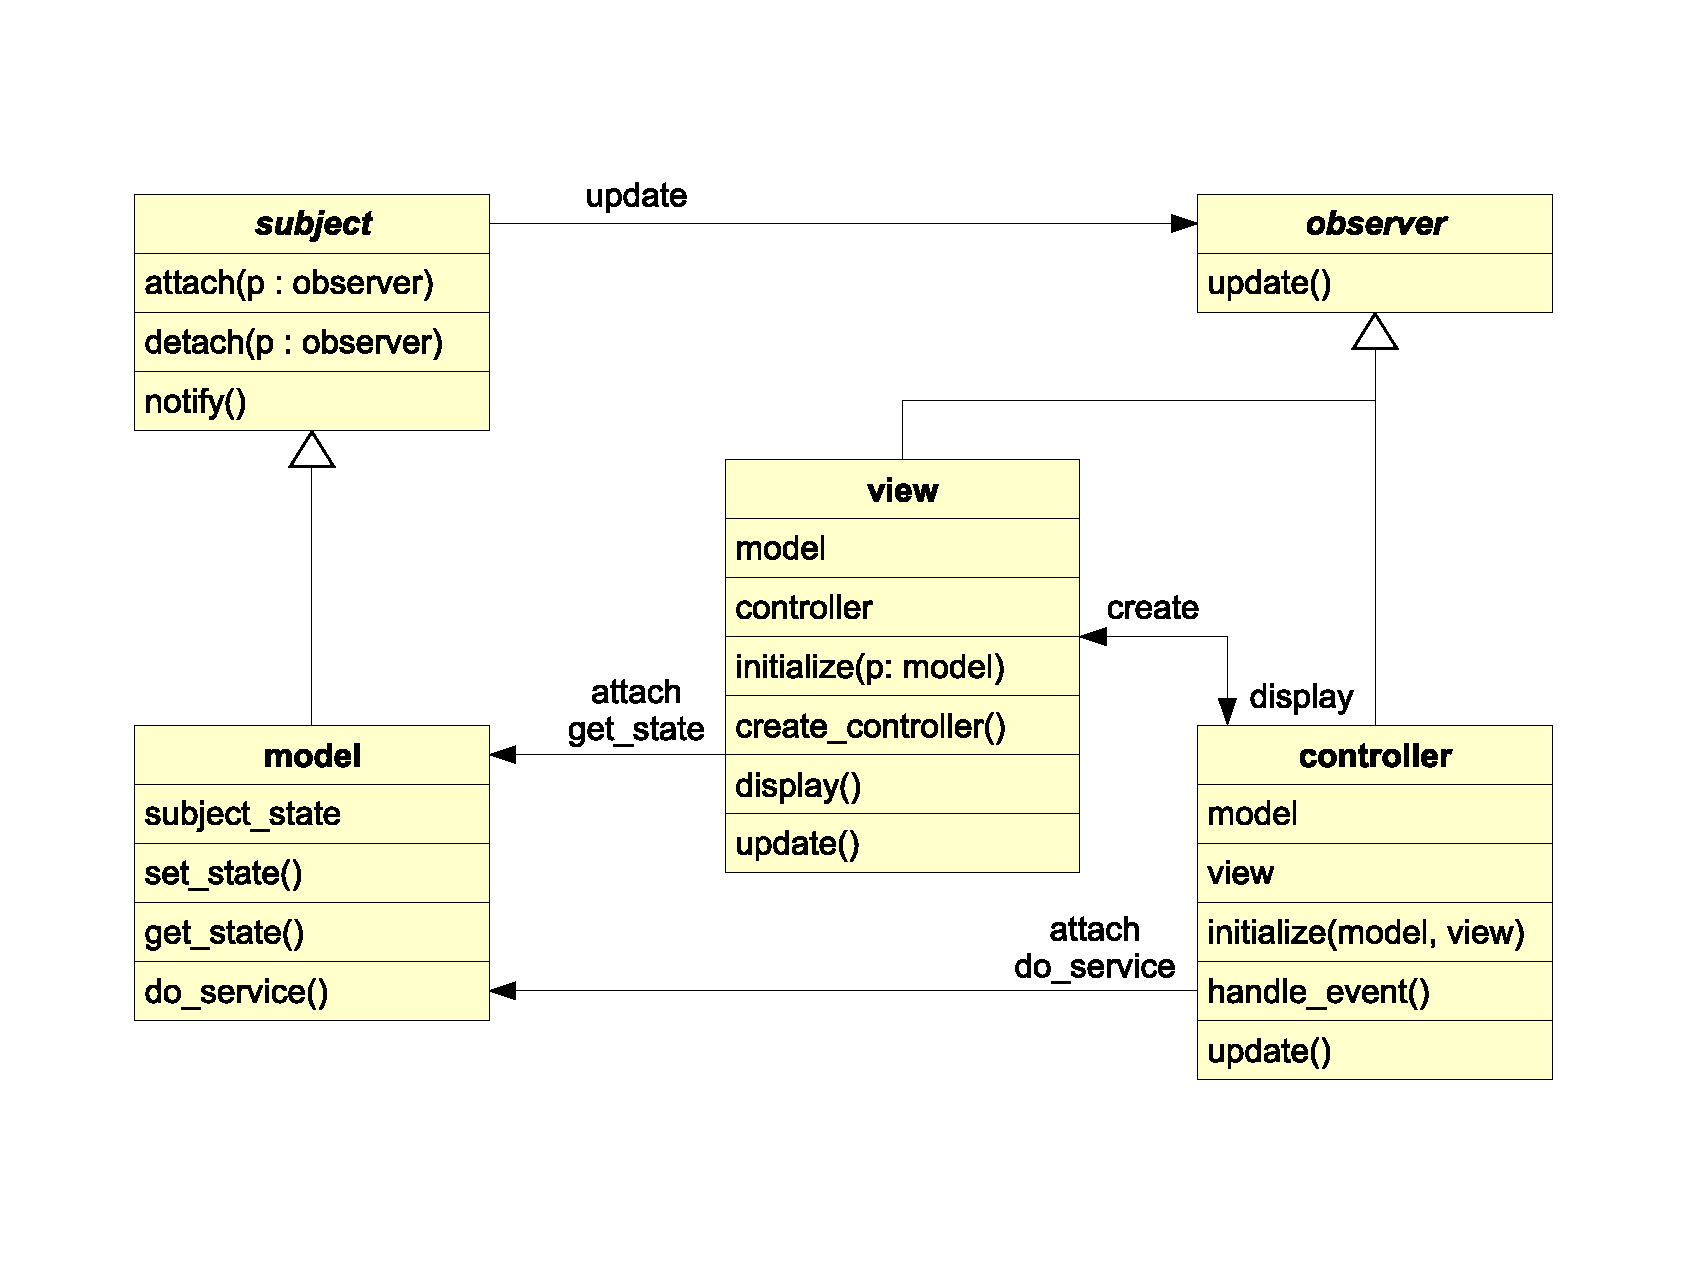
\includegraphics[scale=0.3]{vector/mvcobserver.eps}
        \caption{MVC- using Observer Pattern}
        \label{mvcobserver_figure}
    \end{center}
\end{figure}

Similar notification mechanisms are used for \emph{Callback} event handling in
frameworks, where the framework core calls functionality of its extensions. The
\emph{Model View Controller-} (MVC) uses the \emph{Observer} pattern to let the
model notify its observing views about necessary updates (figure
\ref{mvcobserver_figure}).

A disadvantage of the \emph{Observer} pattern is that it relies on bidirectional
dependencies (section \ref{bidirectional_dependency_heading}), so that circular
references can occur, when a system is not programmed very carefully.

%
% $RCSfile: bidirectional_dependency.tex,v $
%
% Copyright (C) 2002-2008. Christian Heller.
%
% Permission is granted to copy, distribute and/or modify this document
% under the terms of the GNU Free Documentation License, Version 1.1 or
% any later version published by the Free Software Foundation; with no
% Invariant Sections, with no Front-Cover Texts and with no Back-Cover
% Texts. A copy of the license is included in the section entitled
% "GNU Free Documentation License".
%
% http://www.cybop.net
% - Cybernetics Oriented Programming -
%
% http://www.resmedicinae.org
% - Information in Medicine -
%
% Version: $Revision: 1.1 $ $Date: 2008-08-19 20:41:05 $ $Author: christian $
% Authors: Christian Heller <christian.heller@tuxtax.de>
%

\subsubsection{Bidirectional Dependency}
\label{bidirectional_dependency_heading}
\index{Bidirectional Dependency}
\index{Inter-Dependency}
\index{Endless Loop}
\index{Tree}
\index{Directed Acyclic Graph}
\index{DAG}
\index{Oriented Acyclic Graph}
\index{Process Tree}
\index{Object Tree}
\index{Database Data Structure}
\index{File System Structure}
\index{Syntax Tree}
\index{Acyclic Graph}
\index{Circular Reference}

\emph{Bidirectional References} are a nightmare for every software developer.
They cause \emph{Inter-Dependencies} so that changes in one part of a system can
affect multiple other parts which in turn affect the originating part, which may
finally lead to cycles or even endless loops. Also, the actual program flow and
effects of changes to a system become very hard to trace. Therefore, the avoidance
of such dependencies belongs to the core principles of good software design.

A \emph{Tree}, in mathematics, is defined as \textit{Directed Acyclic Graph}
(DAG), also known as \emph{Oriented Acyclic Graph} \cite{nist}. It has a
\emph{Root Node} and \emph{Child Nodes} which can become \emph{Parent Nodes}
when having children themselves; otherwise they are called \emph{Leaves}.
Children of the same node are \emph{Siblings}. \textit{A common constraint is
that no node can have more than one parent}, as \cite{foldoc} writes and
continues: \textit{Moreover, for some applications, it is necessary to consider
a node's children to be an ordered list, instead of merely a set.} A graph is
\emph{acyclic} if every node can be reached via exactly one path, which then
also is the shortest possible.

In computing, trees are used in many forms, for example as \emph{Process Tree}
of an operating system \cite{debian, gnu, linux} or as \emph{Object Tree} of an
object-oriented application. They represent \emph{Data Structures} in databases
or file systems and also the \emph{Syntax Tree} of languages. The violation of
the principle of the \emph{Acyclic Graph} can lead to the same loops, also
called \emph{Circular References}, as mentioned above, which can result in the
crossing of memory limits and is a potential security risk. Therefore, one of
the main aims in the creation of the new concepts introduced in part
\ref{contribution_heading} of this work was the avoidance of bidirectional
relations.


%
% $RCSfile: idiomatic.tex,v $
%
% Copyright (C) 2002-2008. Christian Heller.
%
% Permission is granted to copy, distribute and/or modify this document
% under the terms of the GNU Free Documentation License, Version 1.1 or
% any later version published by the Free Software Foundation; with no
% Invariant Sections, with no Front-Cover Texts and with no Back-Cover
% Texts. A copy of the license is included in the section entitled
% "GNU Free Documentation License".
%
% http://www.cybop.net
% - Cybernetics Oriented Programming -
%
% http://www.resmedicinae.org
% - Information in Medicine -
%
% Version: $Revision: 1.1 $ $Date: 2008-08-19 20:41:07 $ $Author: christian $
% Authors: Christian Heller <christian.heller@tuxtax.de>
%

\subsection{Idiomatic}
\label{idiomatic_heading}
\index{Idiomatic Pattern}
\index{Idiom}
\index{Counted Pointer Pattern}
\index{Singleton Pattern}
\index{Template Method Pattern}
\index{Factory Method Pattern}
\index{Envelope Letter Pattern}

An \emph{Idiom} is a pattern on a low abstraction level. It describes how certain
aspects of components or the relations between them can be implemented using the
means of a specific programming language. Idioms can thus be used to describe
the actual realisation of design patterns. Besides the \emph{Counted-Pointer}
pattern, Buschmann \cite[p. 377]{buschmann} also categorises \emph{Singleton},
\emph{Template Method}, \emph{Factory Method} and \emph{Envelope-Letter}
\cite{coplien} as \emph{Idiom}.

%
% $RCSfile: template_method.tex,v $
%
% Copyright (C) 2002-2008. Christian Heller.
%
% Permission is granted to copy, distribute and/or modify this document
% under the terms of the GNU Free Documentation License, Version 1.1 or
% any later version published by the Free Software Foundation; with no
% Invariant Sections, with no Front-Cover Texts and with no Back-Cover
% Texts. A copy of the license is included in the section entitled
% "GNU Free Documentation License".
%
% http://www.cybop.net
% - Cybernetics Oriented Programming -
%
% http://www.resmedicinae.org
% - Information in Medicine -
%
% Version: $Revision: 1.1 $ $Date: 2008-08-19 20:41:09 $ $Author: christian $
% Authors: Christian Heller <christian.heller@tuxtax.de>
%

\subsubsection{Template Method}
\label{template_method_heading}
\index{Template Method Pattern}
\index{Hook Method Pattern}

The \emph{Template Method} pattern \cite{gamma1995}, also called
\emph{Hook Method}, is an abstract definition of the \emph{Skeleton} of an
algorithm. The implementation of one or more steps of that algorithm is
delegated to a sub class (figure \ref{templatemethod_figure}).

\begin{figure}[ht]
    \begin{center}
        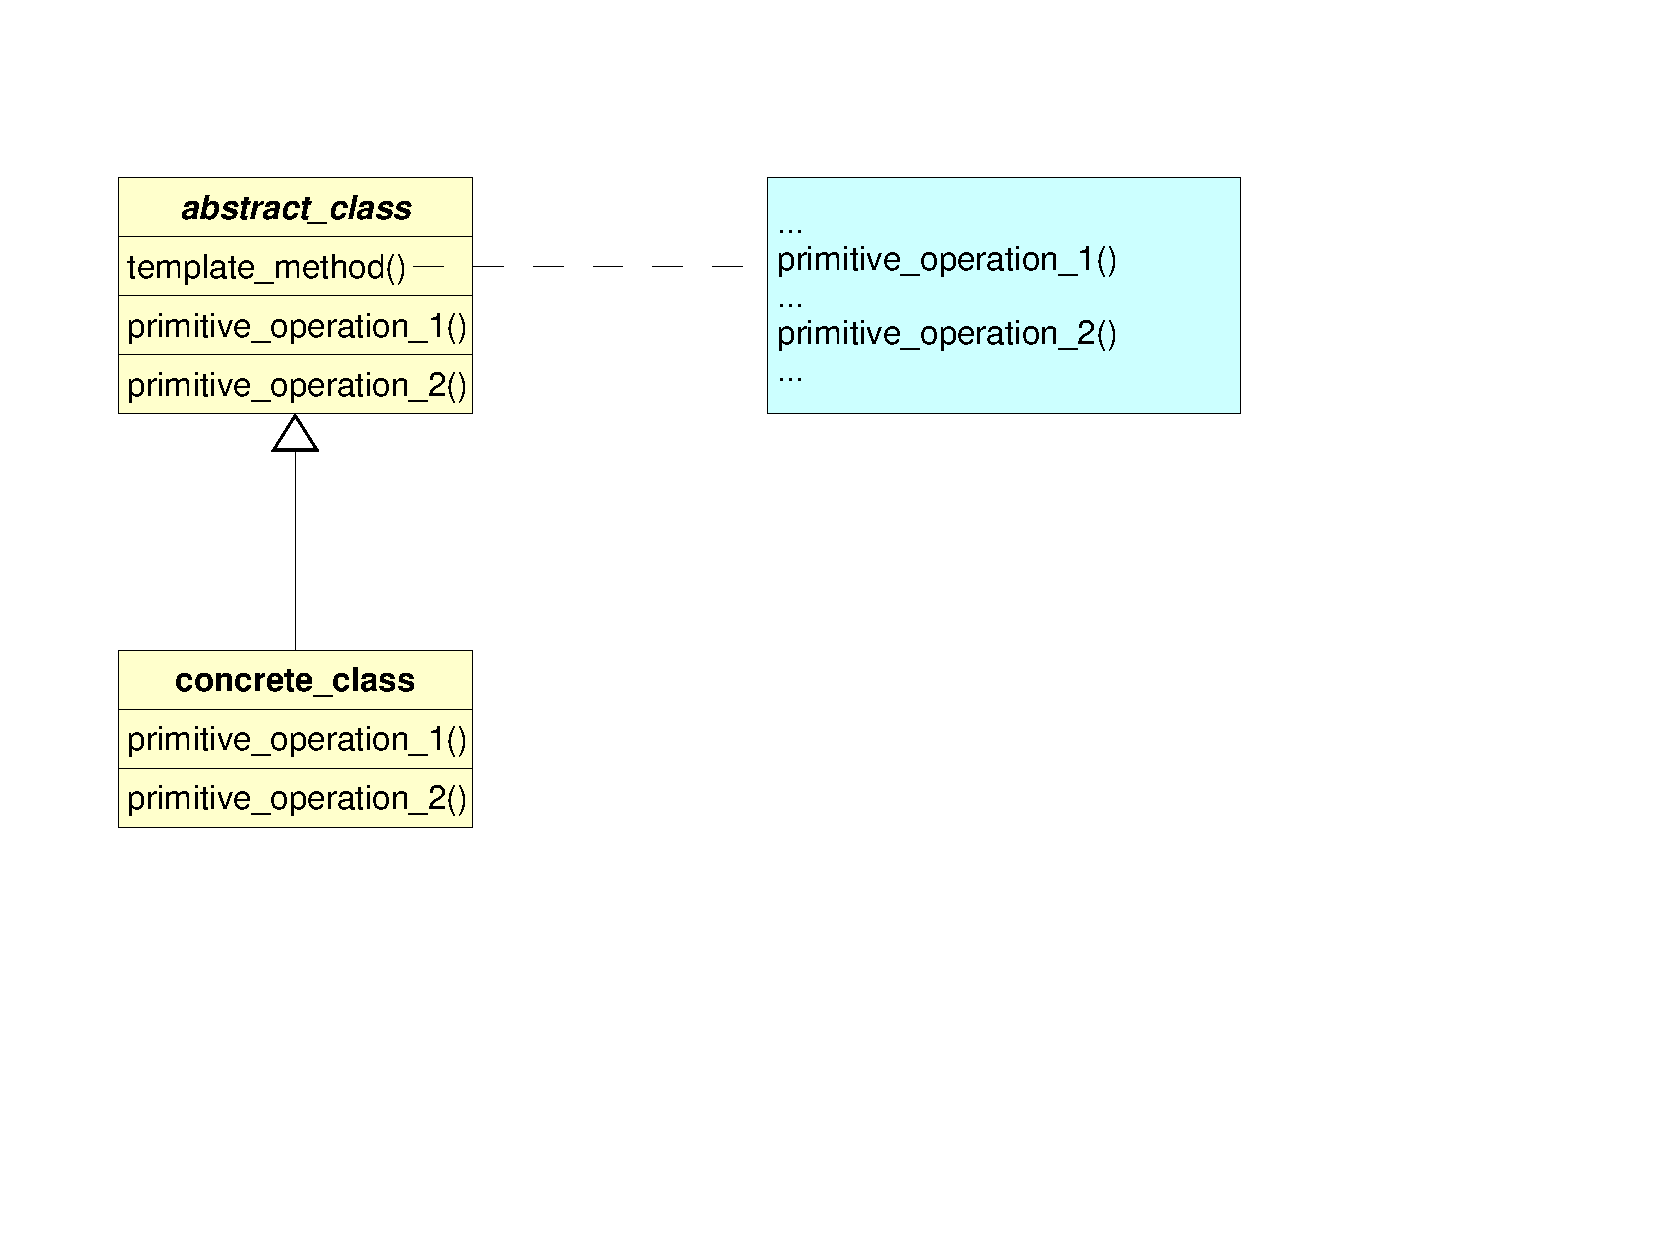
\includegraphics[scale=0.3,angle=-90]{graphic/templatemethod.pdf}
        \caption{Template Method Pattern}
        \label{templatemethod_figure}
    \end{center}
\end{figure}

The idea of algorithm (method) templates was taken over in the design of the
new language described in chapter \ref{cybernetics_oriented_language_heading}.
The single template parts, however, are not inherited but implemented in
\emph{part} templates referenced by their corresponding \emph{whole} template,
which is actually more similar to the previously described \emph{Whole-Part}
pattern (section \ref{design_heading}).

%
% $RCSfile: counted_pointer.tex,v $
%
% Copyright (c) 2004. Christian Heller. All rights reserved.
%
% No copying, altering, distribution or any other actions concerning this
% document, except after explicit permission by the author!
% At some later point in time, this document is planned to be put under
% the GNU FDL license. For now, _everything_ is _restricted_ by the author.
%
% http://www.cybop.net
% - Cybernetics Oriented Programming -
%
% http://www.resmedicinae.org
% - Information in Medicine -
%
% @author Christian Heller <christian.heller@tuxtax.de>
%

\paragraph{Counted Pointer}
\label{counted_pointer_heading}

The \emph{Counted Pointer} pattern \cite{buschmann} supports memory management
in the \emph{C++} programming language, by counting references to dynamically
created objects (figure \ref{pointer_figure}). That way, it can avoid the
destruction of an object through one client, while still being referenced by
other clients. Also, it helps avoiding memory leaks by cleaning up forgotten
objects.

\begin{figure}[ht]
    \begin{center}
        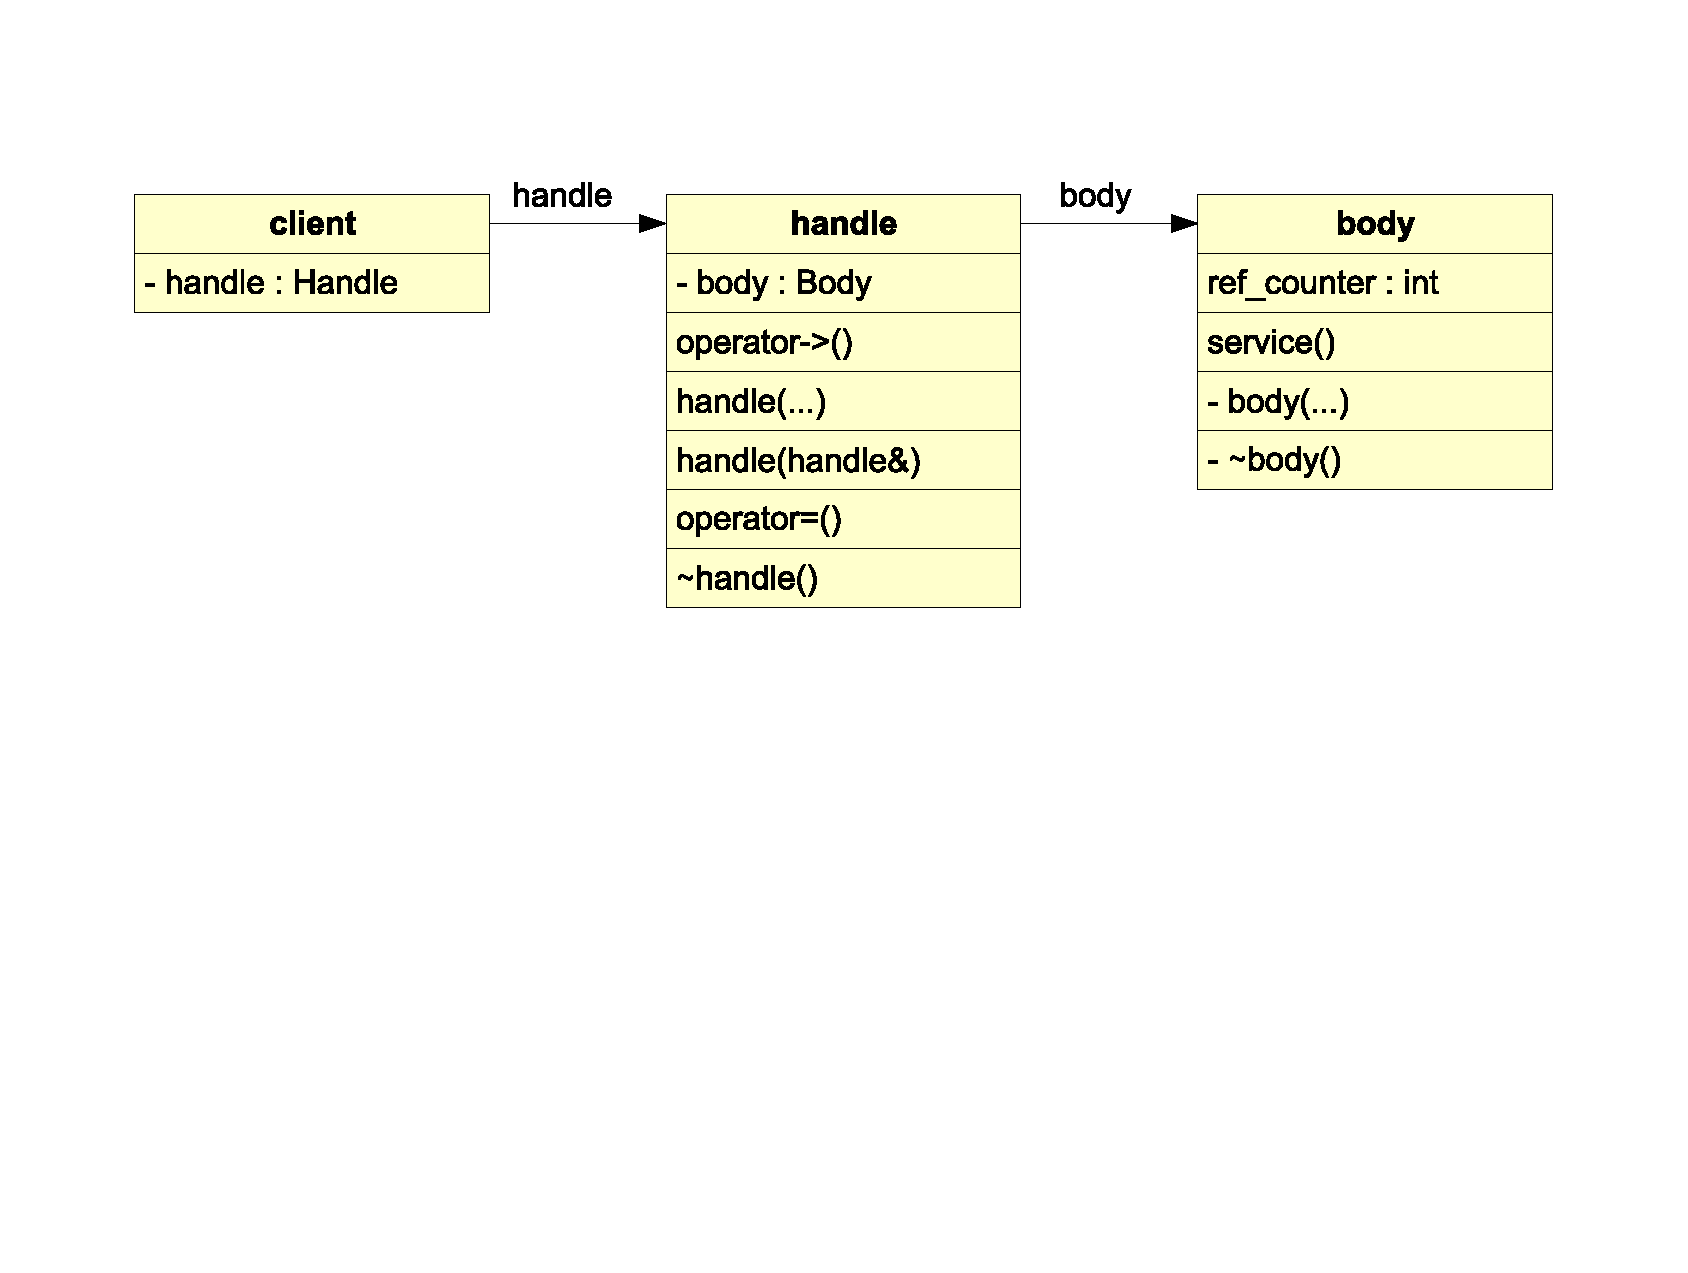
\includegraphics[scale=0.3]{vector/pointer.eps}
        \caption{Counted Pointer Pattern}
        \label{pointer_figure}
    \end{center}
\end{figure}

%
% $RCSfile: singleton.tex,v $
%
% Copyright (C) 2002-2008. Christian Heller.
%
% Permission is granted to copy, distribute and/or modify this document
% under the terms of the GNU Free Documentation License, Version 1.1 or
% any later version published by the Free Software Foundation; with no
% Invariant Sections, with no Front-Cover Texts and with no Back-Cover
% Texts. A copy of the license is included in the section entitled
% "GNU Free Documentation License".
%
% http://www.cybop.net
% - Cybernetics Oriented Programming -
%
% http://www.resmedicinae.org
% - Information in Medicine -
%
% Version: $Revision: 1.1 $ $Date: 2008-08-19 20:41:08 $ $Author: christian $
% Authors: Christian Heller <christian.heller@tuxtax.de>
%

\subsubsection{Singleton}
\label{singleton_heading}
\index{Singleton Pattern}
\index{Global Data Access}
\index{Class Method}
\index{Registry Object Pattern}
\index{Manager Object Pattern}
\index{Lifecycle Method}

Whenever an object-oriented system wants to ensure that only one instance of a
certain class exists, the \emph{Singleton} pattern \cite{gamma1995} can be
used. It essentially is a class which encapsulates its instance's data and
provides global access to them, via \emph{static}, sometimes called
\emph{class} methods (figure \ref{singleton_figure}).

\begin{figure}[ht]
    \begin{center}
        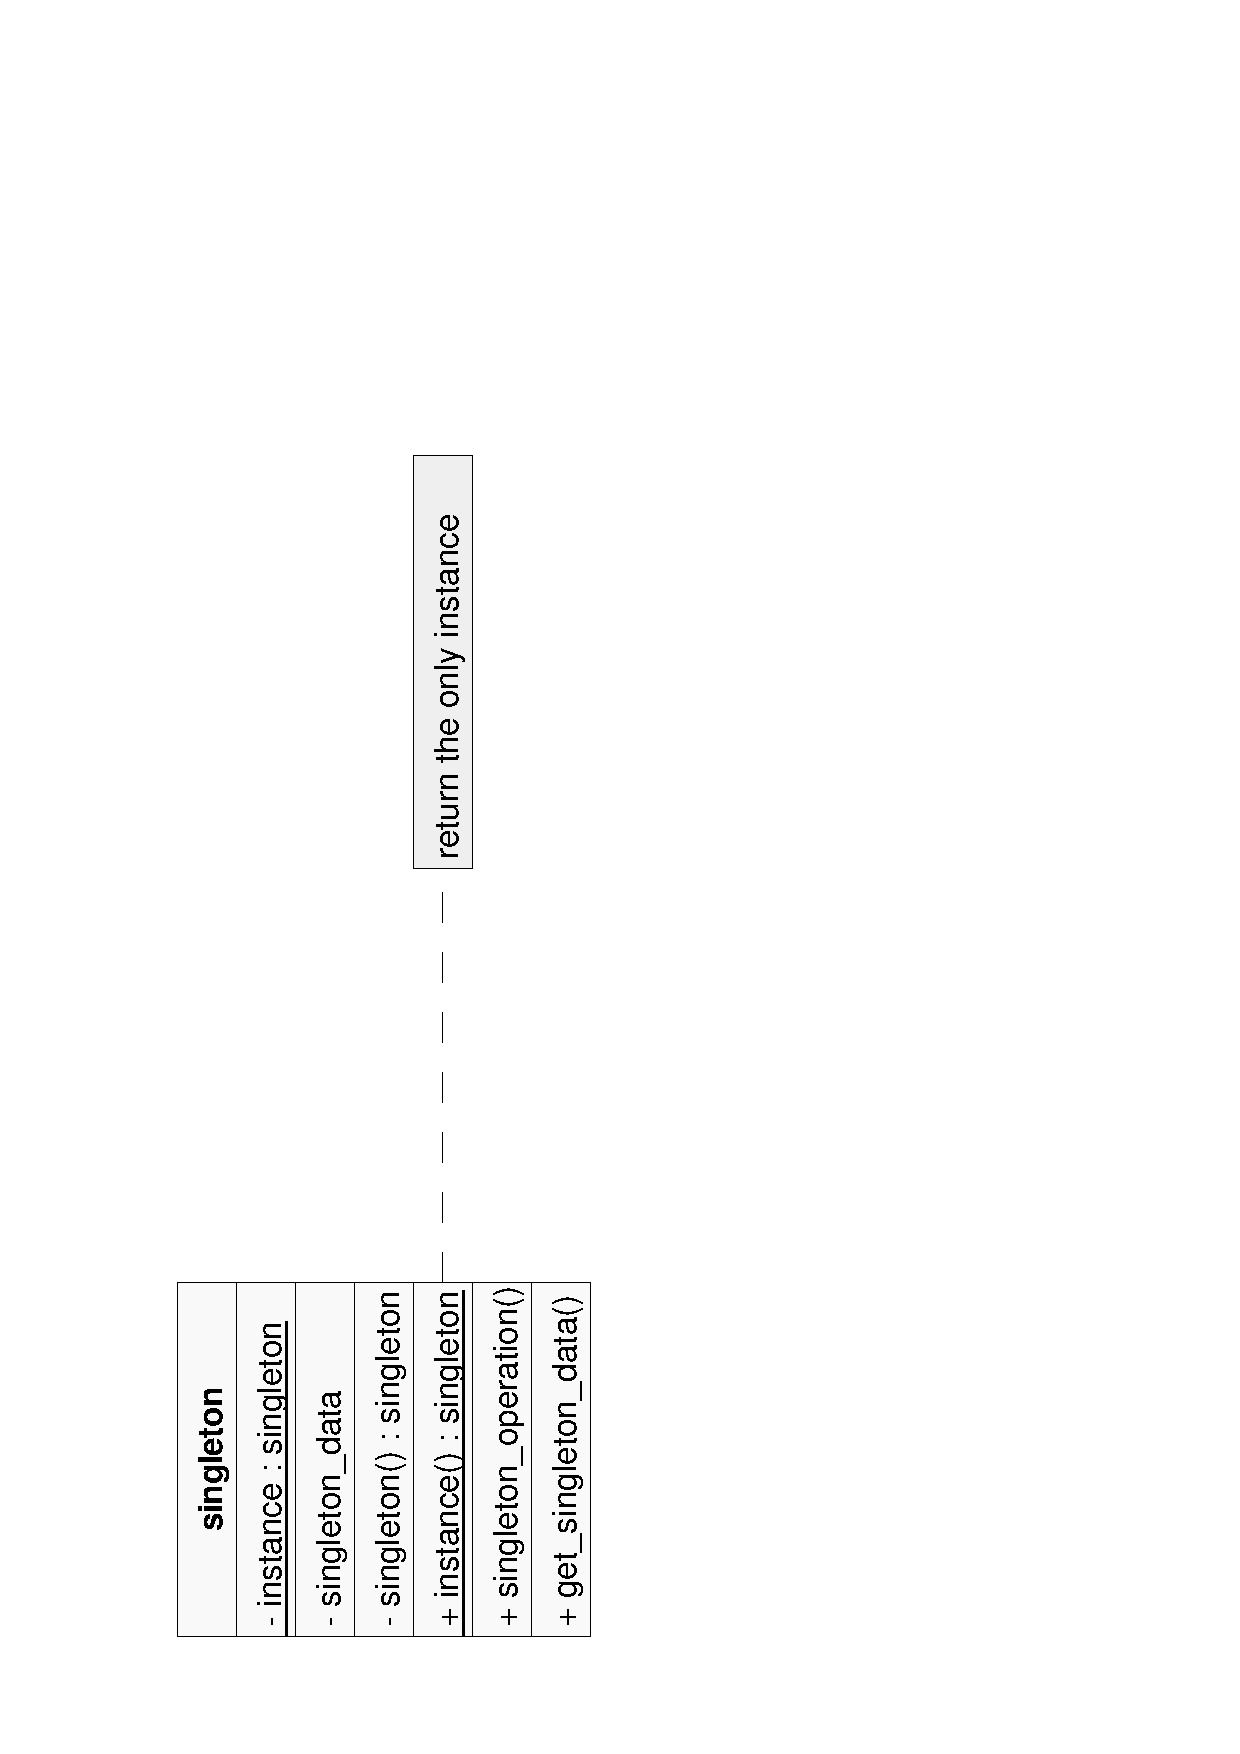
\includegraphics[scale=0.3,angle=-90]{graphic/singleton.pdf}
        \caption{Singleton Pattern}
        \label{singleton_figure}
    \end{center}
\end{figure}

A \emph{Registry} object as described by Fowler \cite{fowler2002} often uses
the \emph{Singleton} pattern, to be unique and to become globally accessible.
Similarly do many so-called \emph{Manager} objects, for example change managers
which are also responsible for the caching of objects.

Global, that is static access -- the main purpose of the \emph{Singleton}
pattern, is its main weakness, at the same time. One obvious solution to avoid
singleton objects could be to forward global information as instances from
component to component, possibly using an own \emph{Lifecycle Method} (section
\ref{component_lifecycle_heading}). This approach, however, might bring with a
rather large number of parameters to be handed over. It therefore seems easier
to use another alternative -- the central tree of knowledge instances, as done
in the interpreter of chapter \ref{cybernetics_oriented_interpreter_heading}.

%
% $RCSfile: global_access.tex,v $
%
% Copyright (c) 2004. Christian Heller. All rights reserved.
%
% No copying, altering, distribution or any other actions concerning this
% document, except after explicit permission by the author!
% At some later point in time, this document is planned to be put under
% the GNU FDL license. For now, _everything_ is _restricted_ by the author.
%
% http://www.cybop.net
% - Cybernetics Oriented Programming -
%
% http://www.resmedicinae.org
% - Information in Medicine -
%
% @author Christian Heller <christian.heller@tuxtax.de>
%

\subsection{Global Access}
\label{global_access_heading}

A pure tree of instances in a computer's \emph{Random Access Memory} (RAM)
represents an unidirectional structure that permits data access along
\emph{well-defined} paths. Global access via static types, on the other hand,
allows \emph{any} instance to address data in memory \emph{directly}, which not
only complicates software development and maintenance, but, due to the
uncontrollable access, is a potential security risk.

The usage of static objects accessible by any other part in a system is an
\emph{Anti Pattern} to \emph{Inversion of Control} (IoC) \cite{avalon}, highly
insecure and hence undesirable.



    \newpage{\pagestyle{empty}\cleardoublepage}
    %
% $RCSfile: diagrams.tex,v $
%
% Copyright (c) 2002-2007. Christian Heller. All rights reserved.
%
% Permission is granted to copy, distribute and/or modify this document
% under the terms of the GNU Free Documentation License, Version 1.1 or
% any later version published by the Free Software Foundation; with no
% Invariant Sections, with no Front-Cover Texts and with no Back-Cover
% Texts. A copy of the license is included in the section entitled
% "GNU Free Documentation License".
%
% http://www.cybop.net
% - Cybernetics Oriented Programming -
%
% Version: $Revision: 1.2 $ $Date: 2007-08-01 13:59:00 $ $Author: christian $
% Authors: Christian Heller <christian.heller@tuxtax.de>
%

\chapter{Diagrams}
\label{diagrams_heading}
\index{Diagrams}
\index{Unified Modeling Language}
\index{UML}
\index{Template Diagram}
\index{TD}
\index{Model Diagram}
\index{MD}
\index{Organisation Diagram}
\index{OD}
\index{Communication Diagram}
\index{CD}

Because of the different programming philosophy behind CYBOP, standard
\emph{Unified Modeling Language} (UML) diagrams cannot be used unalteredly for
the design of CYBOL applications. Some of them, however, could be quite useful,
when adapted a bit. For creating CYBOL applications, the following four can be
considered sufficient. They model the structure of:

\begin{enumerate}
    \item \emph{Template Diagram} (TD): one design-time template (hierarchical,
        ontological concept), with purely unidirectional relations; does not
        illustrate relations between different concepts, as these are only
        established by logic models at runtime; could look like a UML class
        diagram (CsD) or a tree, only that a template may not only represent states,
        but also logic (algorithms, workflows) (figure \ref{template_diagram_figure})
    \item \emph{Model Diagram} (MD): the runtime model tree; comparable to UML
        object diagram, but a simple tree with named nodes would suffice; is
        important because input/ output parameters of operations are given as
        dot-separated paths to runtime knowledge tree models (figure \ref{model_diagram_figure})
    \item \emph{Organisation Diagram} (OD): template directories; could look
        like a UML component- or package diagram or a simple tree (figure \ref{organisation_diagram_figure})
    \item \emph{Communication Diagram} (CD): a network of communicating
        systems, which may run on the same or on different physical machines
        (nodes); could look like a UML distribution diagram; not to be mixed
        up with UML collaboration diagram (figure \ref{communication_diagram_figure})
\end{enumerate}

\begin{figure}[ht]
    \begin{center}
        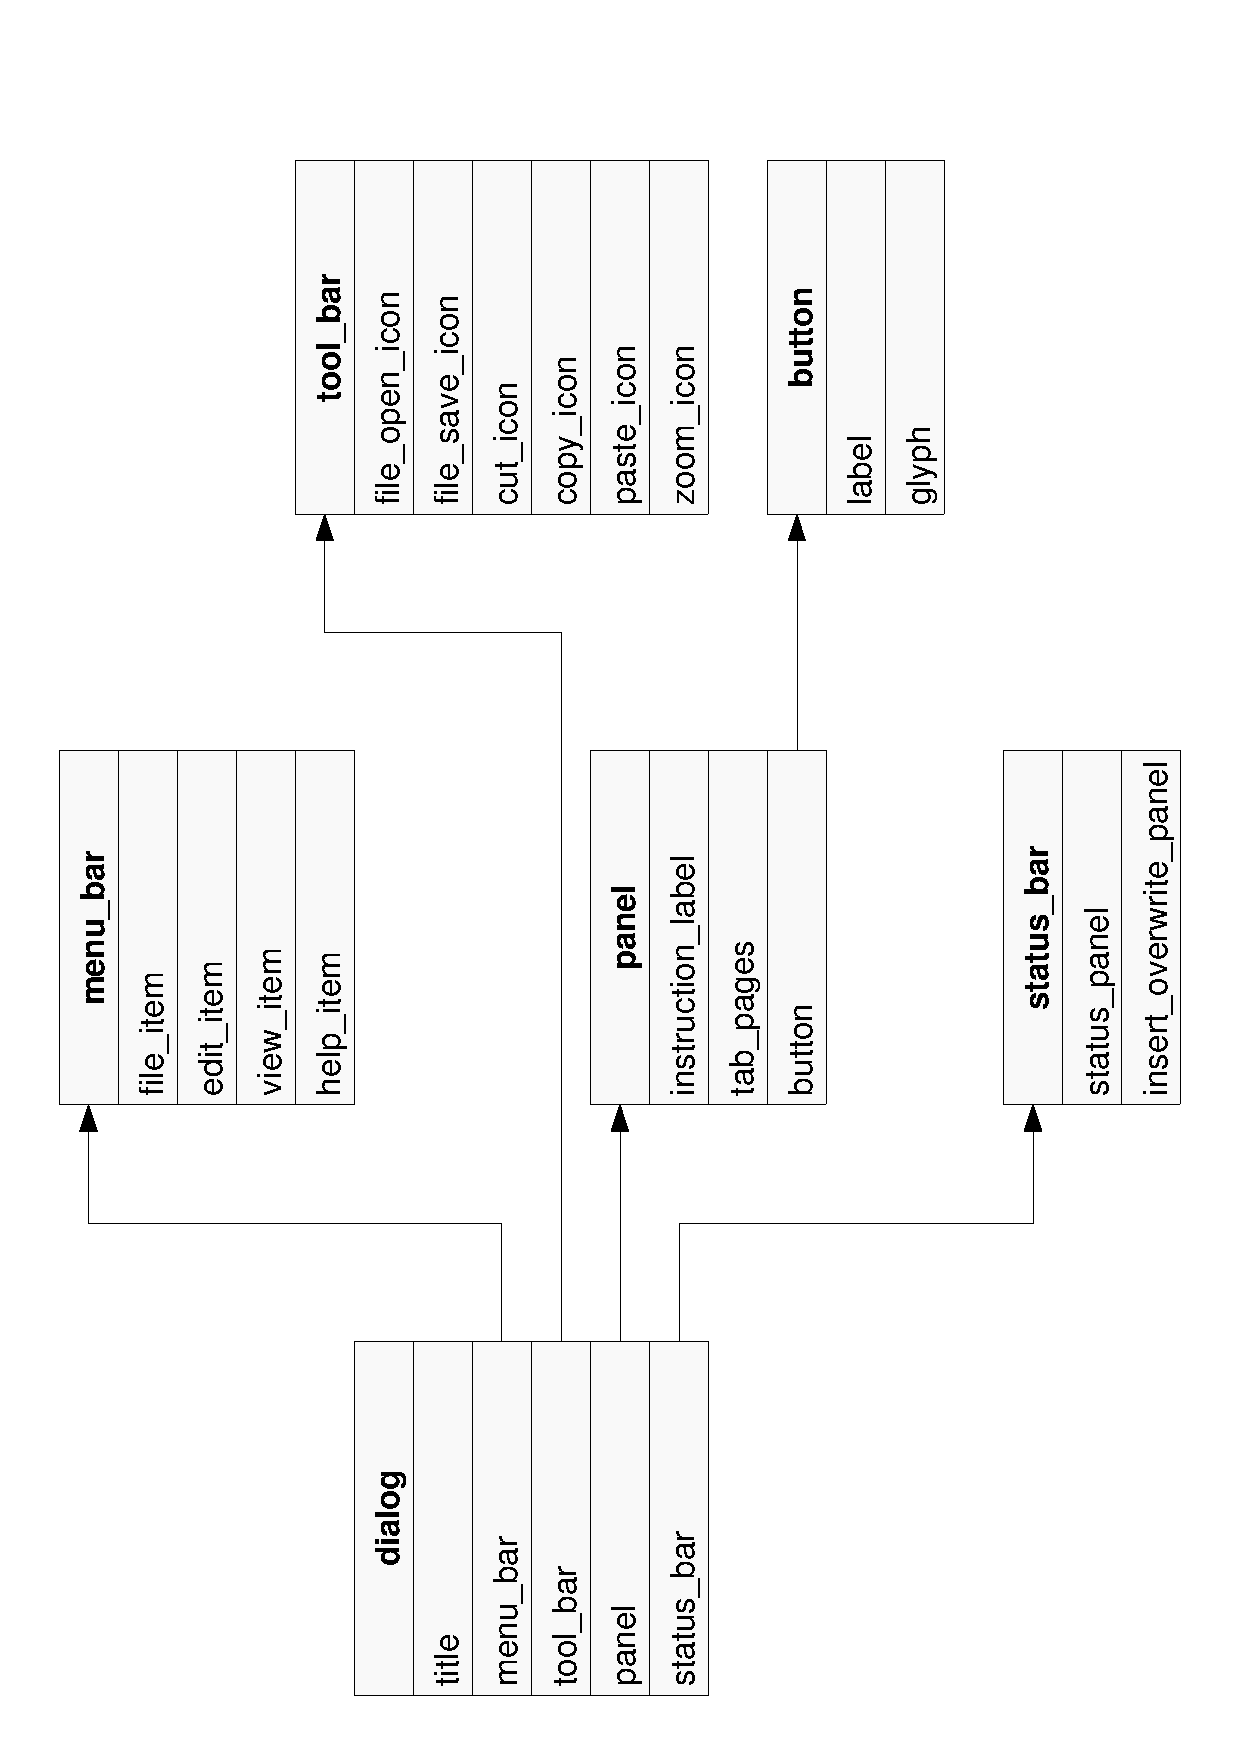
\includegraphics[scale=0.3,angle=-90]{graphics/template_diagram.pdf}
        \caption{CYBOL Template Diagram (TD) Proposal}
        \label{template_diagram_figure}
    \end{center}
\end{figure}

\begin{figure}[ht]
    \begin{center}
        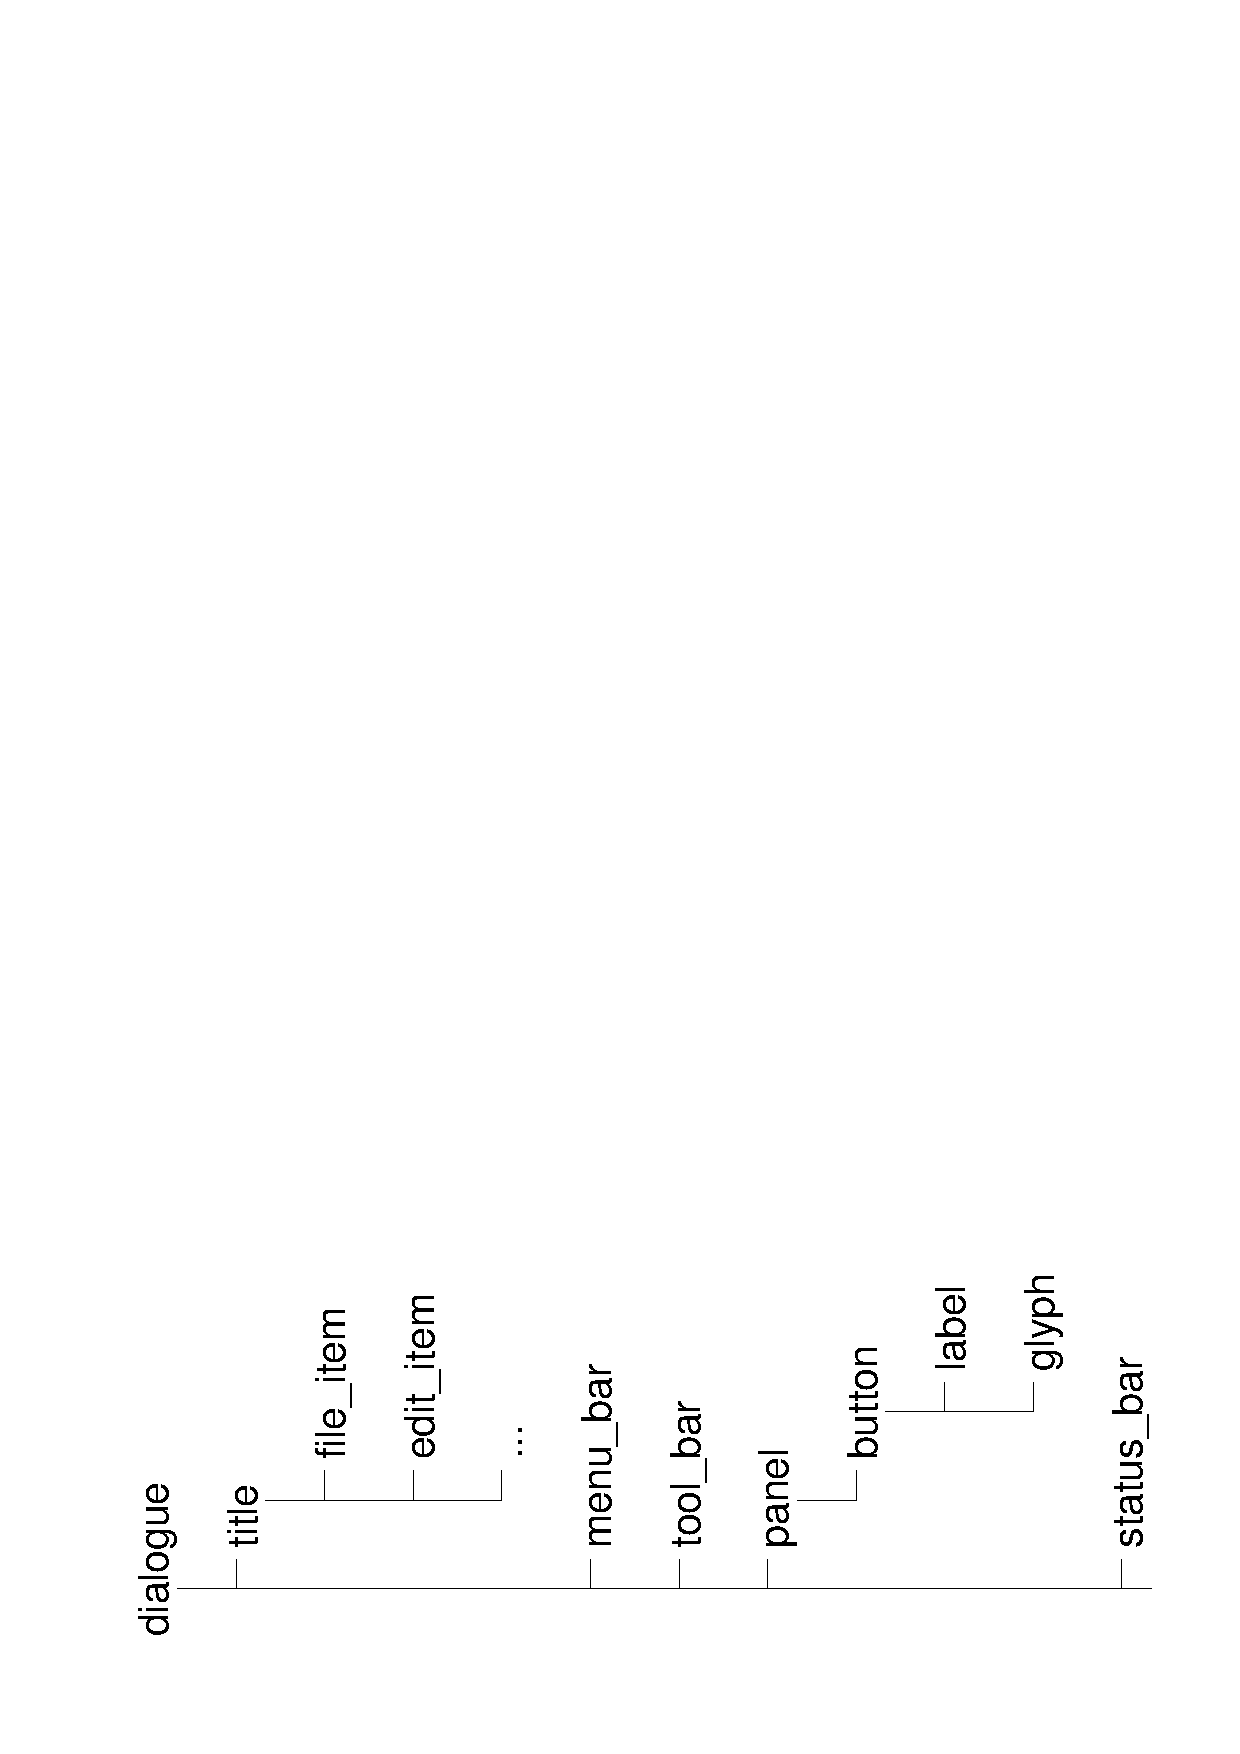
\includegraphics[scale=0.3,angle=-90]{graphics/model_diagram.pdf}
        \caption{CYBOL Model Diagram (MD) Proposal}
        \label{model_diagram_figure}
    \end{center}
\end{figure}

\clearpage

As said above, the four diagrams may look similar to their corresponding UML
pendant. One possible proposal is given for each diagram type. The TD in figure
\ref{template_diagram_figure} illustrates a graphical dialogue. The diagram
looks pretty similar to a UML CsD. Attributes and methods are not bundled in
one concept though, and inheritance does not exist. Associations are drawn if a
concept links to an external concept which may reside in another file (like the
\emph{menu\_bar}), for example. If a part (like the \emph{title}) is hold
inline in the concept, on the other hand, an association is not displayed. Upon
clicking on a part in a concept box, a dialogue opens up that allows the entry
of meta data like the part's channel, abstraction, model and further properties
(details).

The MD in figure \ref{model_diagram_figure} displays the runtime models that were
instantiated with knowledge templates providing the initial values. Again, the
parts of a graphical dialogue were used.

\begin{figure}[ht]
    \begin{center}
        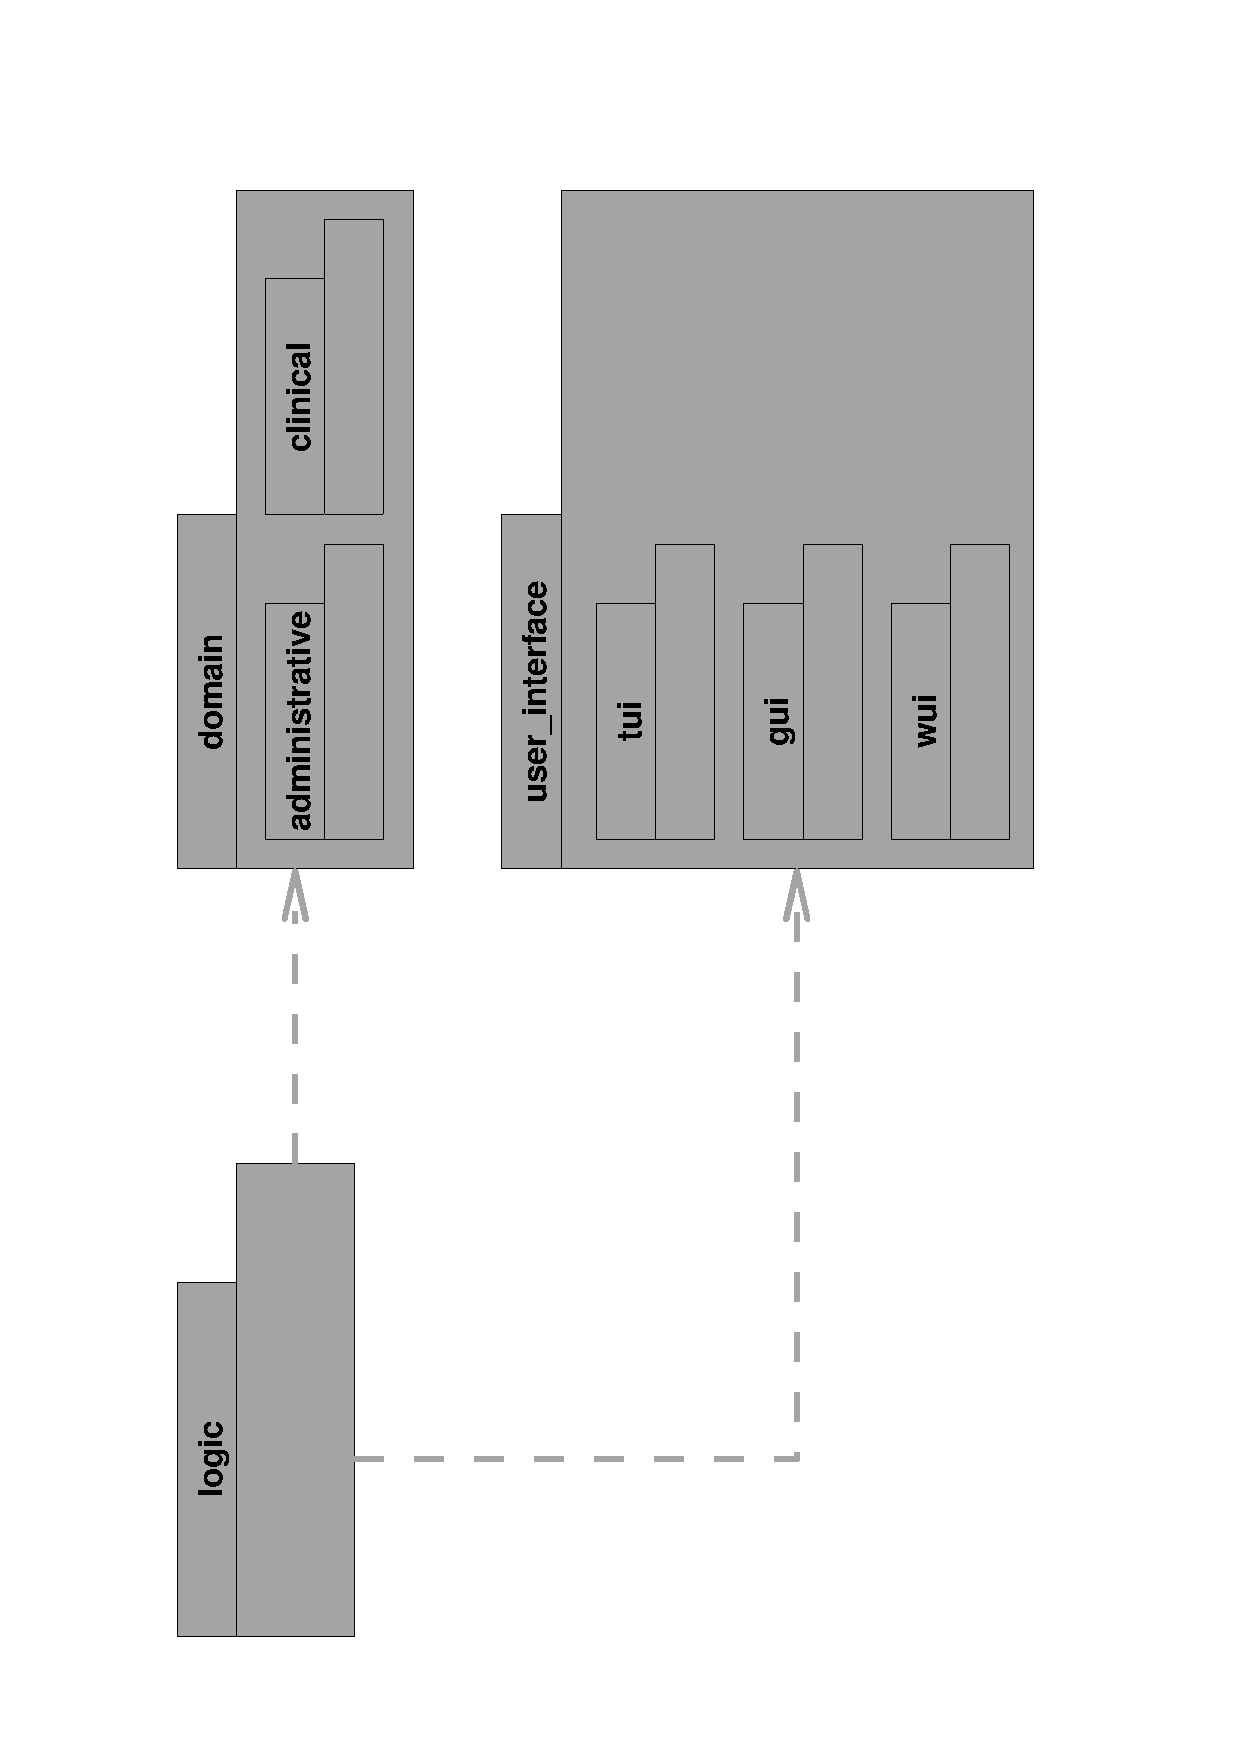
\includegraphics[scale=0.3,angle=-90]{graphics/organisation_diagram.pdf}
        \caption{CYBOL Organisation Diagram (OD) Proposal}
        \label{organisation_diagram_figure}
    \end{center}
\end{figure}

The OD in figure \ref{organisation_diagram_figure} shows packages into which CYBOL knowledge
templates may be organised. Packages do normally correspond to directories on
file system level. The figure contains a \emph{domain} package consisting of
two sub packages, one containing knowledge templates for \emph{administrative}
patient data and the other holding templates for \emph{clinical} data of a
patient. Also, there is a \emph{User Interface} (UI) package containing three
sub packages, for: \emph{Textual UI} (TUI), \emph{Graphical UI} (GUI) and
\emph{Web UI} (WUI). Both, \emph{domain-} as well as \emph{user\_interface}
packages may be accessed from the operations residing in the \emph{logic}
package.

\begin{figure}[ht]
    \begin{center}
        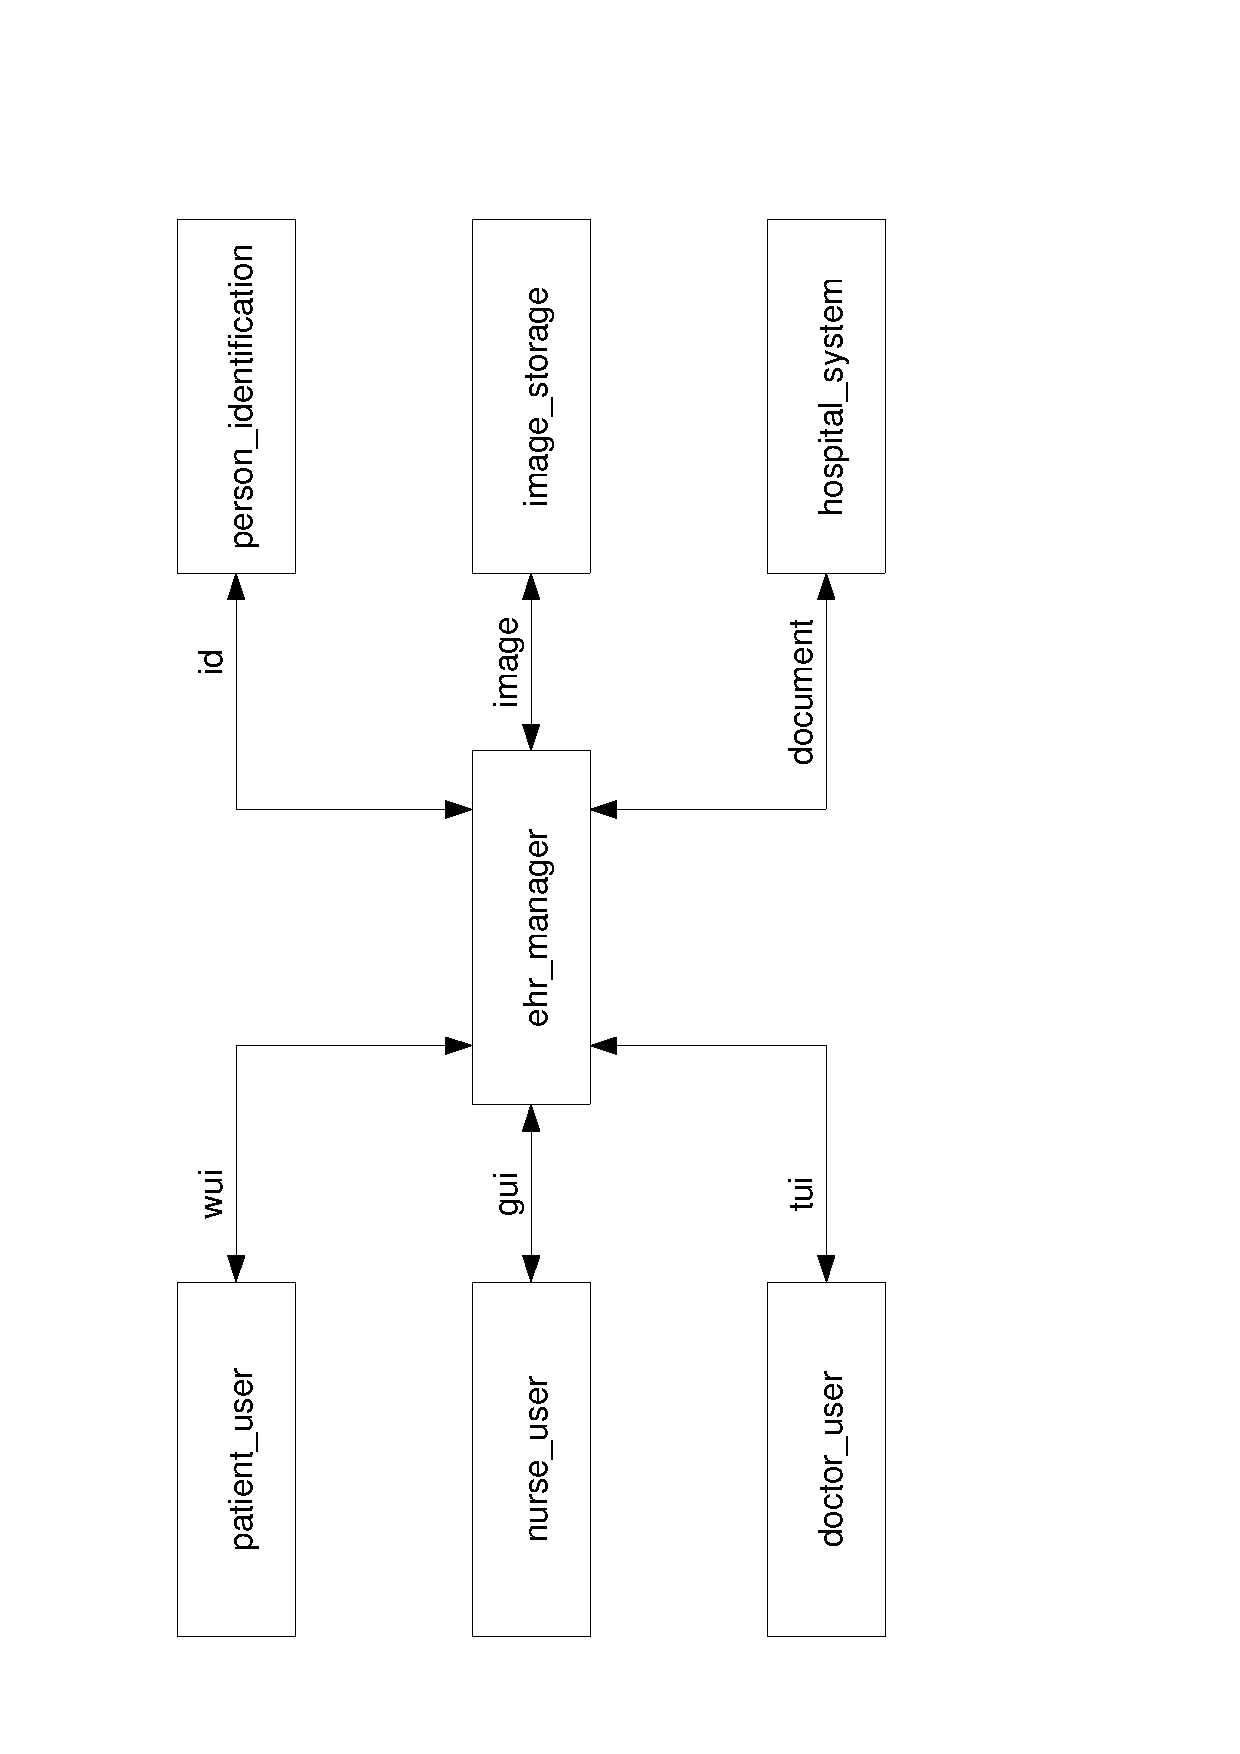
\includegraphics[scale=0.3,angle=-90]{graphics/communication_diagram.pdf}
        \caption{CYBOL Communication Diagram (CD) Proposal}
        \label{communication_diagram_figure}
    \end{center}
\end{figure}

The CD in figure \ref{communication_diagram_figure}, finally, shows a number of independent systems
communicating with each other. An \emph{Electronic Health Record} (EHR) manager
application may be found in the center of the figure. Patients communicate with
it using a WUI; nurses using a GUI and doctors using a TUI (for better
performance). A patient gets identified by asking a \emph{person\_identification}
service. Documents may be exchanged with a \emph{hospital\_system} and images
with a special \emph{image\_storage} system.

    \newpage{\pagestyle{empty}\cleardoublepage}
    %
% $RCSfile: appendices.tex,v $
%
% Copyright (c) 2002-2007. Christian Heller. All rights reserved.
%
% Permission is granted to copy, distribute and/or modify this document
% under the terms of the GNU Free Documentation License, Version 1.1 or
% any later version published by the Free Software Foundation; with no
% Invariant Sections, with no Front-Cover Texts and with no Back-Cover
% Texts. A copy of the license is included in the section entitled
% "GNU Free Documentation License".
%
% http://www.cybop.net
% - Cybernetics Oriented Programming -
%
% Version: $Revision: 1.2 $ $Date: 2007-08-01 13:59:00 $ $Author: christian $
% Authors: Christian Heller <christian.heller@tuxtax.de>
%

\chapter{Appendices}
\label{appendices_heading}

%
% $RCSfile: abbreviations.tex,v $
%
% Copyright (c) 2002-2007. Christian Heller. All rights reserved.
%
% Permission is granted to copy, distribute and/or modify this document
% under the terms of the GNU Free Documentation License, Version 1.1 or
% any later version published by the Free Software Foundation; with no
% Invariant Sections, with no Front-Cover Texts and with no Back-Cover
% Texts. A copy of the license is included in the section entitled
% "GNU Free Documentation License".
%
% http://www.cybop.net
% - Cybernetics Oriented Programming -
%
% Version: $Revision: 1.1 $ $Date: 2007-07-17 20:02:36 $ $Author: christian $
% Authors: Christian Heller <christian.heller@tuxtax.de>
%

%
% More abbreviations can be found at:
%
% http://www.ownnetwork.mfluhr.de/Glossar.htm
% http://www.ciw.uni-karlsruhe.de/abklex.html
% http://www.sans.org/resources/glossary.php
% http://www.cknow.com/ckinfo/acro_d/dde_1.shtml
% http://filext.com/
% http://forum.europa.eu.int/Public/irc/dsis/coded/info/data/abbreviations/en/all.htm
% http://www.sheilapantry.com/figuk/acronyms.html
% http://sir.cyivs.cy.edu.tw/~hchung/computerabbreviation.htm
% http://dmi-www.mc.duke.edu/dukemi/acronyms.htm (healthcare standards)
%

\section[Abbreviations]{Abbreviations}
\label{abbreviations_heading}

\begin{tabbing}
    \hspace{1cm} \= \hspace{2cm} -- \= \hspace{1.5cm}\= \kill

%    \>3GL \>\>Third Generation Language\\

%    \>4GL \>\>Fourth Generation Language\\

%    \>a/c \>\>account\\

%    \>a/o \>\>account of\\

%    \>a/v \>\>ad valorem (according to value)\\

%    \>AAFP \>\>American Academy of Family Physicians\\

%    \>AAP \>\>American Academy of Pediatrics\\

%    \>ABDA \>\>Bundesvereinigung Deutscher Apotheker Verbaende\\

%    \>ACAP \>\>Application Control Access Protocol\\

%    \>ACID \>\>Atomicity, Consistency, Isolation, Durability\\

%    \>ACL \>\>Access Control List\\

%    \>ACL \>\>Agent Communication Language\\

%    \>ACM \>\>Association for Computing Machinery\\

%    \>ACR \>\>American College of Radiology\\

%    \>ad fin. \>\>ad finem\\

%    \>ad inf. \>\>ad infinitem\\

%    \>ad int. \>\>ad interim\\

%    \>ad lib. \>\>ad libitum\\

%    \>ad loc. \>\>ad locum\\

%    \>AD \>\>Activity Diagram\\

%    \>ADA \>\>American Dental Association\\

%    \>ADL \>\>Archetype Definition Language\\

%    \>ADL \>\>Architecture Description Language\\

%    \>ADO \>\>ActiveX Data Object\\

%    \>ADSL \>\>Asymmetrical DSL\\

%    \>ADT \>\>Abrechnungs DT\\

%    \>AE \>\>Application Engineering\\

%    \>AE \>\>Automation Engineering\\

%    \>AGOP \>\>Agent Oriented Programming\\

%    \>AI \>\>Artificial Intelligence\\

%    \>AID \>\>Application ID\\

%    \>AIDS \>\>Anomaly-based IDS\\

%    \>ALU \>\>Arithmetic Logic Unit\\

%    \>AM \>\>Access Mode\\

%    \>AM \>\>Archetype Model\\

%    \>AMA \>\>American Medical Association\\

%    \>AMR \>\>Automated Medical Record\\

%    \>ANN \>\>Artificial Neural Network\\

%    \>ANSI \>\>American National Standards Institute\\

%    \>AODT \>\>Ambulant Operieren DT\\

%    \>AOP \>\>Aspect Oriented Programming\\

%    \>AOSD \>\>Aspect Oriented SD\\

%    \>API \>\>Application Programming Interface\\

%    \>ARP \>\>Address Resolution Protocol\\

%    \>ARQ \>\>Automatic Repeat Request\\

%    \>ARR \>\>Access Rule Reference\\

%    \>ASCII \>\>American Standard Code for Information Interchange\\

%    \>ASD \>\>Adaptive Software Development\\

%    \>ASE \>\>Application Service Element\\

%    \>ASIC \>\>Application Specific IC\\

%    \>ASN \>\>Abstract Syntax Notation\\

%    \>ASP \>\>Active Server Pages\\

%    \>ASP \>\>Application Service Provider\\

%    \>ASTM \>\>American Society for Testing and Materials\\

%    \>AT \>\>AUT Template\\

%    \>ATM \>\>Asynchronous Transfer Mode\\

%    \>ATP \>\>Appletalk Transaction Protocol\\

%    \>ATR \>\>Answer to Reset\\

%    \>AUT \>\>Authentication\\

%    \>AVI \>\>Audio Video Interleave\\

%    \>AWT \>\>Abstract Window Toolkit\\

%    \>B-ISDN \>\>Broadband ISDN\\

%    \>B2B \>\>Business to Business\\

%    \>BASIC \>\>Beginners All purpose Symbolic Instruction Code\\

%    \>B.C. \>\>before Christ\\

%    \>BCD \>\>Binary Coded Decimal\\

%    \>BCDIC \>\>BCD Interchange Code\\

%    \>BDT \>\>Behandlungs DT\\

%    \>BeOS \>\>Be, Inc. OS\\

%    \>BER \>\>Basic Encoding Rules\\

%    \>BIOS \>\>Basic I/O System\\

%    \>Bit \>\>Binary Digit\\

%    \>BLOB \>\>Binary LOB\\

%    \>BMC \>\>BioMed Central\\

%    \>BNF \>\>Backus Naur Form\\

%    \>BO \>\>Business Object\\

%    \>BOOTP \>\>BOOTstrap Protocol\\

%    \>BSD \>\>Berkeley Software (System) Distribution (Design)\\

%    \>C \>\>Certificate\\

%    \>c/o \>\>care of\\

%    \>c/s \>\>client/ server\\

%    \>C.O.D. \>\>Cash on Delivery\\

%    \>CA \>\>Certification Authority\\

%    \>CAD \>\>Computer Aided Design\\

%    \>cADL \>\>Constraint Form of ADL\\

%    \>CAM \>\>Computer Aided Manufacturing\\

%    \>CAP \>\>College of American Pathologists\\

%    \>CAPI \>\>Common ISDN Application Programming Interface\\

%    \>CAR \>\>CA Reference\\

%    \>CASE \>\>Computer Aided Software Engineering\\

%    \>CASE \>\>Common ASE\\

%    \>CBC \>\>Cipher Block Chaining\\

%    \>CBD \>\>Component Based Design (Development)\\

%    \>CBO \>\>Community Based Organisation\\

%    \>CC \>\>Cryptographic Checksum\\

%    \>CCR \>\>Continuity of Care Record\\

%    \>CCT \>\>CC Template\\

%    \>CD \>\>Certificate Directory\\

%    \>CD \>\>Collision Detection\\

%    \>CD \>\>Communication Diagram\\

%    \>CDA \>\>Clinical Document Architecture\\

%    \>CDB \>\>Check Digit Byte\\

%    \>CDDI \>\>Copper Distributed Data Interface\\

%    \>CDISC \>\>Clinical Data Interchange Standards Consortium\\

%    \>CEN \>\>Comite Europeen de Normalisation\\
%        \>\>\>(European Committee for Standardisation)\\

%    \>CENELEC \>\>CEN Electrotechnique\\
%        \>\>\>(European Committee for Electrotechnical Standardisation)\\

%    \>CEO \>\>Chief Executive Officer\\

%    \>CEPT \>\>European Conference of Post and Telecommunication Administrations\\

%    \>CERN \>\>Conseil Europeen pour le Recherche Nucleaire\\

%    \>CertSign \>\>Certificate Signing\\

%    \>CG \>\>Cryptogram\\

%    \>CGI \>\>Common Gateway Interface\\

%    \>CH \>\>Card Holder\\

%    \>CHA \>\>Certificate Holder Authorisation\\

%    \>CHR \>\>Certificate Holder Reference\\

%    \>CIAC \>\>Computer Incident Advisory Capability\\

%    \>CIAS \>\>Clinical Image Access Service\\

%    \>CICS \>\>Customer Information Control System\\

%    \>CII \>\>Computer Implemented Inventions\\

%    \>CIR \>\>Committed Information Rate\\

%    \>CISC \>\>Complex Instruction Set Computing\\

%    \>CL \>\>Common Lisp\\

%    \>CLM \>\>Connectionless Service\\

%    \>CLNP \>\>Connectionless Network Layer Protocol\\

%    \>CLNS \>\>Connectionless Network Service\\

%    \>CLOS \>\>Common Lisp Object System\\

%    \>CLSI \>\>Clinical and Laboratory Standards Institute\\

%    \>CMC \>\>Computer Mediated Communication\\

%    \>CMC \>\>Common Mail Calls\\

%    \>CmD \>\>Component Diagram\\

%    \>CMET \>\>Common Message Element Type\\

%    \>CMM \>\>Capability Maturity Model\\

%    \>CMMI \>\>Capability Maturity Model Integration\\

%    \>CMR \>\>Computerised Medical Record\\

%    \>CMS \>\>Content Management System\\

%    \>CMS \>\>Card Management System\\

%    \>CNS \>\>Central NS\\

%    \>COAS \>\>Clinical Observations Access Service\\

%    \>COBOL \>\>Common Business Oriented Language\\

%    \>CoD \>\>Communication (Collaboration) Diagram\\

%    \>COM \>\>Component Object Model\\

%    \>COM \>\>Connection-Oriented Service\\

%    \>COO \>\>Chief Operating Officer\\

%    \>COP \>\>Component Oriented Programming\\

%    \>CORBA \>\>Common ORB Architecture\\

%    \>COS \>\>Card OS\\

%    \>CP/M \>\>Control Program for Microprocessors\\
%        \>\>\>(Control Program/ Monitor)\\

%    \>CPI \>\>Certificate Profile ID\\

%    \>CPR \>\>Computer-based Patient Record\\
%        \>\>\>(Computerised Patient Record)\\

%    \>CPT \>\>Current Procedural Terminology\\

%    \>CPRI \>\>CPR Institute\\

%    \>CPRS \>\>CPR System\\

%    \>CPU \>\>Central Processing Unit\\

%    \>CR \>\>CEN Report\\

%    \>CRC \>\>Class, Responsibilities, Collaborations\\

%    \>CRC \>\>Cyclic Redundancy Check\\

%    \>CRC \>\>Cyclic Redundancy Code\\

%    \>CRM \>\>Common Reference Model\\

%    \>CS \>\>CertSign\\

%    \>CsD \>\>Class Diagram\\

%    \>CSD \>\>Composite Structure Diagram\\

%    \>CSMA \>\>Carrier Sensing Multiple Access\\

%    \>CSMA/CA \>\>Carrier Sensing Multiple Access with Collision Avoidance\\

%    \>CSMA/CD \>\>Carrier Sensing Multiple Access with Collision Detection\\

%    \>CSP \>\>Certificate Service Provider\\

%    \>CSS \>\>Cascading Style Sheet\\

%    \>CSV \>\>Comma Separated Variable\\

%    \>CT \>\>Computer Tomograph\\

%    \>CTV3 \>\>Clinical Terms Version 3\\

%    \>CVS \>\>Concurrent Versions System\\

%    \>CWA \>\>CEN Working Agreement\\

%    \>CWM \>\>Common Warehouse Metamodel\\

    \>CYBOI \>\>Cybernetics Oriented Interpreter\\

    \>CYBOL \>\>Cybernetics Oriented Language\\

%    \>CYBOM \>\>Cybernetics Oriented Methodology\\

    \>CYBOP \>\>Cybernetics Oriented Programming\\

%    \>CYBORG \>\>Cybernetic Organism\\

%    \>CYBOS \>\>Cybernetics Oriented Operating System\\

%    \>CYBOX \>\>Cybernetics Oriented Box\\

%    \>dADL \>\>Data Definition Form of ADL\\

%    \>DAG \>\>Directed Acyclic Graph\\

%    \>DAML \>\>DARPA Agent ML\\

%    \>DAO \>\>Data Access Object\\

%    \>DARPA \>\>Defense Advanced Research Projects Agency\\

%    \>DB \>\>Database\\

%    \>DB2 \>\>DB 2\\

%    \>DBMS \>\>DB Management System\\

%    \>DCC \>\>Direct Client to Client Protocol\\

%    \>DCD \>\>Document Content Description\\

%    \>DCE \>\>Distributed Computing Environment\\

%    \>DCE \>\>Data Circuit-Terminating Equipment\\
 � �%    \>\>\>(Data Communications Equipment)\\

%    \>DCL \>\>Data Control Language\\

%    \>DCOM \>\>Distributed COM\\

%    \>DD \>\>Deployment Diagram\\

%    \>DDE \>\>Dynamic Data Exchange\\

%    \>DDL \>\>Data Definition Language\\

%    \>DDoS \>\>Distributed Denial of Service\\

%    \>DDP \>\>Datagram Delivery Protocol\\

%    \>DE \>\>Domain Engineering\\

%    \>DEB \>\>Debian GNU/Linux Package\\

%    \>DES \>\>Data Encryption Standard\\

%    \>DFN \>\>Deutsches Forschungsnetz\\

%    \>DHTML \>\>Dynamic HTML\\

%    \>DICOM \>\>Digital Imaging and Communications in Medicine\\

%    \>DIF \>\>Data Interchange Format\\

%    \>DIMDI \>\>Deutsches Institut fuer Medizinische Dokumentation und Information\\

%    \>DIMSE \>\>DICOM Message Service Element\\

%    \>DIN \>\>Deutsches Institut fuer Normung\\

%    \>DIR \>\>Directory\\

%    \>DLC \>\>Dynamic Link Control\\

%    \>DLL \>\>Dynamic Link Library\\

%    \>DML \>\>Data Manipulation Language\\

%    \>DMP \>\>Disease Management Programme\\

%    \>DMR \>\>Digital Medical Record\\

%    \>DNA \>\>Desoxy Ribo Nucleic Acid\\

%    \>DNA \>\>Distributed interNet Application Architecture\\

%    \>DNR \>\>Do Not Resuscitate\\

%    \>DNS \>\>Domain Name Service\\
%        \>\>\>(Domain Name System)\\

%    \>DOM \>\>Document Object Model\\

%    \>DOS \>\>Disk OS\\

%    \>DPMI \>\>DOS Protected Mode Interface\\

%    \>DQDB \>\>Distributed Queue Dual Bus\\

%    \>DSDM \>\>Dynamic System Development Method\\

%    \>DS \>\>Digital Signature\\

%    \>DSI \>\>DS Input\\

%    \>DSL \>\>Digital Subscriber Line\\

%    \>DSL \>\>Domain Specific Language\\

%    \>DSOM \>\>Distributed System Object Model\\

%    \>DSP \>\>Digital Signal Processor\\

%    \>DSSSL \>\>Document Style Semantics and Specification Language\\

%    \>DST \>\>DS Template\\

%    \>DT \>\>Datentraeger\\

%    \>DTD \>\>Document Type Definition\\

%    \>DTE \>\>Data Termination Equipment\\

%    \>DTO \>\>Data Transfer Object\\

%    \>DVI \>\>Device Independent\\

%    \>DVI \>\>Digital Video Interface\\

%    \>e.g. \>\>exempli gratia (for example)\\

%    \>EAA \>\>Enterprise Application Architecture\\

%    \>EBCDIC \>\>Extended BCDIC\\

%    \>EBES \>\>European Board of EDI Standardisation\\

%    \>EBNF \>\>Extended BNF\\

%    \>EC \>\>Existential Conjunctive\\

%    \>ECC \>\>Error Correction Code\\
%        \>\>\>(Error Checking and Correction)\\

%    \>ECML \>\>Electronic Commerce Modeling Language\\

%    \>ED \>\>Emergency Department\\

%    \>EDI \>\>Electronic Data Interchange\\

%    \>EDIF \>\>EDI Format\\

%    \>EDIFACT \>\>EDI for Administration, Commerce and Transport\\

%    \>EDP \>\>Electronic Data Processing\\

%    \>EEG \>\>EBES Expert Group\\

%    \>EEPROM \>\>Electrically Erasable Programmable ROM\\

%    \>EET \>\>Encyclopedia of Educational Technology\\

%    \>EGP \>\>Exterior Gateway Protocol\\

%    \>eHC \>\>Electronic Health Card\\

%    \>EHCR \>\>Electronic Health Care Record\\

%    \>EHR \>\>Electronic Health Record\\

%    \>EHRcom \>\>EHR Communications\\

%    \>EIA \>\>Electronic Industries Alliance\\

%    \>EICAR \>\>European Institute for Computer Anti-Virus Research\\

%    \>EIR \>\>Electronic Insurance Record\\

%    \>EJB \>\>Enterprise Java Bean\\

%    \>EMA \>\>Electronic Messaging Association\\

%    \>EMI \>\>Electronic Medical Infrastructure\\

%    \>EMR \>\>Electronic Medical Record\\

%    \>EN \>\>European Standard\\

%    \>ENV \>\>European Prestandard\\

%    \>EOF \>\>End of File\\

%    \>EPR \>\>Electronic Patient Record\\

%    \>EPS \>\>Encapsulated PS\\

%    \>ER \>\>Endoplasmic Reticulum\\

%    \>ERD \>\>Entity Relationship Diagram\\

%    \>ERM \>\>Entity Relationship Model\\

%    \>ERP \>\>Enterprise Resource Planning\\

%    \>et al. \>\>et alii (and others)\\

%    \>etc. \>\>et cetera (and so on)\\

%    \>ETH \>\>Eidgenoessische Technische Hochschule\\

%    \>ETSI \>\>European Telecommunications Standards Institute\\

%    \>EU \>\>European Union\\

%    \>EUD \>\>End User Development\\

%    \>Extended ML \>\>Extended Meta Language\\

%    \>FAQ \>\>Frequently Asked Question\\

%    \>FAX \>\>Facsimile Transmission\\

%    \>FBO \>\>Faith Based Organisation\\

%    \>FDD \>\>Feature Driven Development\\

%    \>FDDI \>\>Fiber Distributed Data Interface\\

%    \>FDL \>\>Free Documentation License\\

%    \>FeatuRSEB \>\>Feature RSEB\\

%    \>FEC \>\>Forward Error Correction\\

%    \>FHS \>\>Filesystem Hierarchy Standard\\

%    \>FIC \>\>Family of International Classifications\\

%    \>FIFO \>\>First In, First Out\\

%    \>FLOSS \>\>Free/ Libre OSS\\

%    \>FODA \>\>Feature Oriented Domain Analysis\\

%    \>FOLDOC \>\>Free On-line Dictionary of Computing\\

%    \>FOPL \>\>First Order Predicate Logic\\

%    \>FORE \>\>Family Oriented Requirements Engineering\\

%    \>FOSS \>\>Free and OSS\\

%    \>FPGA \>\>Field Programmable Gate Array\\

%    \>FPU \>\>Floating Point Unit\\

%    \>FQN \>\>Fully Qualified Name\\

%    \>FR \>\>Frame Relay\\

%    \>FRAD \>\>FR Access Device\\

%    \>FSF \>\>Free Software Foundation\\

%    \>FTAM \>\>File Transfer, Access and Management\\

%    \>FTP \>\>File Transfer Protocol\\

%    \>GA \>\>Genetic Algorithm\\

%    \>GALEN \>\>Generalised Architecture for Languages,\\
%        \>\>\>Encyclopaedias and Nomenclatures in Medicine\\

%    \>GAN \>\>Global Area Network\\

%    \>GC \>\>Garbage Collector\\

%    \>GCC \>\>GNU�Compiler Collection\\
%        \>\>\>(GNU C�Compiler)\\

%    \>GDI \>\>Graphics Device Interface\\

%    \>GDT \>\>Geraete DT\\

%    \>GEHR \>\>Good European/ EHR\\

%    \>GEMATIK \>\>Gesellschaft fuer Telematikanwendungen der Gesundheitskarte\\

%    \>GGP \>\>Gateway-to-Gateway Protocol\\

%    \>GIF \>\>Graphics Interchange Format\\

%    \>GIMP \>\>General (GNU) Image Manipulation Program\\

%    \>GMDN \>\>Global Medical Device Nomenclature\\

%    \>GNOME \>\>GNU Network Object Model Environment\\

%    \>GNU \>\>GNU is not UNIX\\

%    \>GoF \>\>Gang of Four\\

%    \>GP \>\>Generative Programming\\

%    \>GP \>\>General Practitioner\\

%    \>GPF \>\>General Protection Fault\\

%    \>GPIC \>\>General Purpose Information Component\\

%    \>GPL \>\>General Public License\\

%    \>GPL \>\>General Purpose Language\\

%    \>GPS \>\>Global Positioning System\\

%    \>GRAIL \>\>GALEN Representation and Integration Language\\

%    \>GTK \>\>GIMP Toolkit\\

%    \>GUI \>\>Graphical UI\\

%    \>GUID \>\>Globally Unique ID\\

%    \>h/w \>\>Hardware\\

%    \>HAL \>\>Hardware Abstraction Layer\\

%    \>HBCI \>\>Homenanking Computer Interface\\

%    \>HCI \>\>Human-Computer Interaction\\

%    \>HD \>\>Harmonisation Document\\

%    \>HDD \>\>Hard Disk Drive\\

%    \>HDL \>\>Hardware Description Language\\

%    \>HDLC \>\>High level Data Link Control\\

%    \>HDTF \>\>Healthcare Domain Task Force\\

%    \>HIDS \>\>Host based IDS\\

%    \>HIMSS \>\>Health Information Management and Systems Society\\

%    \>HIPAA \>\>Healthcare Insurance Portability and Accountability Act\\

%    \>HIS \>\>Hospital Information System\\

%    \>HL7 \>\>Health Level Seven\\

%    \>HMVC \>\>Hierarchical MVC\\

%    \>HOWTO \>\>How To? (Subject Specific Help)\\

%    \>HP \>\>Hewlett Packard\\

%    \>HPC \>\>Health Professional Card\\

%    \>HPTC \>\>High Performance Technical Computing\\

%    \>HTML \>\>Hypertext ML\\

%    \>HTTP \>\>Hypertext Transfer Protocol\\

%    \>HTTP-ng \>\>HTTP next generation\\

%    \>HTTPD \>\>HTTP Daemon\\

%    \>HTTPS \>\>HTTP over SSL\\

%    \>HUK \>\>Haftpflicht-Unterstuetzungs-Kasse Coburg\\

%    \>HW \>\>Hardware\\

%    \>HXP \>\>Healthcare Xchange Protocol\\

%    \>i/e \>\>import/ export\\

%    \>i/o \>\>input/ output\\

%    \>i/p \>\>input\\

%    \>IABG \>\>Industrieanlagen-Betriebsgesellschaft\\

%    \>ib. \>\>ibidem (in the same place)\\

%    \>ibid. \>\>ib.\\

%    \>IBM \>\>International Business Machines\\

%    \>i/c \>\>in charge of\\

%    \>IC \>\>Integrated Circuit\\

%    \>ICC \>\>IC Card\\

%    \>ICCSN \>\>ICC SN\\

%    \>ICANN \>\>Internet Corporation for Assigned Names and Numbers\\

%    \>ICD \>\>International Classification of Diseases\\

%    \>ICF \>\>International Classification of Functioning, Disability and Health\\

%    \>ICHI \>\>International Classification of Health Interventions\\

%    \>ICHPPC \>\>International Classification of Health Problems in Primary Care\\

%    \>ICMP \>\>Internet Control Message Protocol\\

%    \>ICN \>\>International Council of Nurses\\

%    \>ICNP \>\>International Classification for Nursing Practice (Procedures)\\

%    \>ICQ \>\>I seek you\\

%    \>ICR \>\>Integrated Care Record\\

%    \>ICPC \>\>International Classification of Primary Care\\

%    \>id. \>\>idem (the same)\\

%    \>ID \>\>Identifier\\

%    \>IDE \>\>Integrated Development Environment\\

%    \>IDEA \>\>International Data Encryption Algorithm\\

%    \>IDL \>\>Interface Definition Language\\

%    \>IDS \>\>Intrusion Detection System\\

%    \>i.e. \>\>id est (that is)\\

%    \>IEEE \>\>Institute of Electrical and Electronics Engineers\\

%    \>IETF \>\>Internet Engineering Task Force\\

%    \>IGMP \>\>Internet Group Management Protocol\\

%    \>IGP \>\>Interior Gateway Protocol\\

%    \>IIIS \>\>International Institute of Informatics and Systemics\\

%    \>IIM \>\>Internet Interaction Management\\

%    \>IIOP \>\>Internet Inter ORB Protocol\\

%    \>IIS \>\>Internet Information Server\\

%    \>IM \>\>Information Model\\

%    \>IMAP \>\>Internet Message Access Protocol\\

%    \>IMP \>\>Interface Message Processor\\

%    \>IMTC \>\>International Multimedia Teleconferencing Consortium\\

%    \>Inc. \>\>Incorporated\\

%    \>InterNIC \>\>Internet Network Information Center\\

%    \>IoC \>\>Inversion of Control\\

%    \>IOD \>\>Interaction Overview Diagram\\

%    \>IOM \>\>Institute of Medicine\\

%    \>IP \>\>Internet Protocol\\

%    \>IPC \>\>Inter-Process Communication\\

%    \>IPv6 \>\>Internet Protocol (Version 6)\\

%    \>IPX \>\>Internet Packet Exchange\\

%    \>IRC \>\>Internet Relay Chat\\

%    \>IRQ \>\>Interrupt Request\\

%    \>IS \>\>International Standard\\

%    \>ISA \>\>Instruction Set Architecture\\

%    \>ISBD \>\>International Standard Book Description\\

%    \>ISDN \>\>Integrated Services Digital Network\\

%    \>ISO \>\>International Organization for Standardization\\

%    \>ISP \>\>Internet Service Provider\\

%    \>IST \>\>Information Science Technology\\

%    \>IT \>\>Information Technology\\

%    \>ITC \>\>MIT Internet \& Telecoms Convergence Consortium\\

%    \>ITU \>\>International Telecommunication Union\\

%    \>J2EE \>\>Java 2 Platform Enterprise Edition\\

%    \>JAR \>\>Java Archive\\

%    \>JDBC \>\>Java DB Connectivity\\

%    \>JDK \>\>Java Development Kit\\

%    \>JEDEC \>\>Joint Electron Device Engineering Council\\

%    \>JFC \>\>Java Foundation Classes\\

%    \>JMS \>\>Java Message Service\\

%    \>JNDI \>\>Java Naming and Directory Interface\\

%    \>JNI \>\>Java Native Interface\\

%    \>JOSMC \>\>Journal of Free and Open Source Medical Computing\\

%    \>JPE \>\>Java Platform for the Enterprise\\

%    \>JPEG \>\>Joint Photographic Experts Group\\

%    \>JPM \>\>Join Point Model\\

%    \>jr. \>\>junior\\

%    \>JSP \>\>Java Server Pages\\

%    \>JTM \>\>Job Transfer and Management (Manipulation)\\

%    \>JTS \>\>Java Transaction Service\\

%    \>JVM \>\>Java VM\\

%    \>KBV \>\>Kassenaerztliche Bundesvereinigung\\

%    \>KDE \>\>K Desktop Environment\\

%    \>KDT \>\>Kommunikations DT\\

%    \>KE \>\>Knowledge Engineering\\

%    \>KE \>\>Key Encipherment\\

%    \>KEI \>\>KE Input\\

%    \>KID \>\>Key ID\\

%    \>KIF \>\>Knowledge Interchange Format\\

%    \>KIS \>\>Krankenhaus Informations System\\

%    \>KMU \>\>Kleines oder Mittelst\"andisches Unternehmen\\

%    \>KQML \>\>Knowledge Query and Manipulation Language\\

%    \>KV \>\>Kassenaerztliche Vereinigung\\

%    \>KVDT \>\>KV DT\\

%    \>l.c. \>\>loco citato (in the place cited)\\

%    \>L2F \>\>Layer 2 Forwarding\\

%    \>L2TP \>\>Layer 2 Tunneling Protocol\\

%    \>LAN \>\>Local Area Network\\

%    \>LAMP \>\>Linux, Apache, MySQL, PHP/ Perl/ Python\\

%    \>LAMPS \>\>LAMP and SSL\\

%    \>LAPB \>\>Link Access Procedure balanced\\

%    \>LAPD \>\>Link Access Procedure D-channel\\

%    \>LAPM \>\>Link Access Procedure for Modems\\

%    \>LaTeX \>\>Lamport TeX\\

%    \>LDAP \>\>Lightweight Directory Access Protocol\\

%    \>LDR \>\>Lifetime Data Repository\\

%    \>LDT \>\>Labor DT\\

%    \>LGPL \>\>Lesser GPL\\

%    \>LIFO \>\>Last In, First Out\\

%    \>LILO \>\>Linux Loader\\

%    \>LLC \>\>Logical Link Control\\

%    \>LOB \>\>Large Object\\

%    \>LOINC \>\>Logical Observation Identifiers, Names and Codes\\

%    \>LQS \>\>Lexicon (Terminology) Query Service\\

%    \>LRC \>\>Longitudinal Redundancy Check\\

%    \>LSB \>\>Least Significant Byte\\

%    \>Ltd. \>\>limited\\

%    \>LTM \>\>Long Term Memory\\

%    \>LUG \>\>Linux User Group\\

%    \>M. Sc. \>\>Master of Science\\

%    \>MAC \>\>Media Access Control\\

%    \>MAN \>\>Metropolitan Area Network\\

%    \>MAPI \>\>Message Application Programming Interface\\

%    \>MAS \>\>Multi Agent System\\

%    \>MathML \>\>Mathematical ML\\

%    \>MATLAB \>\>Matrix Laboratory\\

%    \>MBR \>\>Master Boot Record\\

%    \>MD \>\>Model Diagram\\

%    \>MD \>\>Medical Doctor\\

%    \>MDA \>\>Model Driven Architecture\\

%    \>MDI \>\>Multiple Document Interface\\

%    \>MeSH \>\>Medical Subject Headings\\

%    \>MFC \>\>MS Foundation Classes\\

%    \>MIF \>\>Management Information Format\\

%    \>MIME \>\>Multipurpose Internet Mail Extension\\

%    \>MIS \>\>Management Information System\\

%    \>MIT \>\>Massachusetts Institute of Technology\\

%    \>ML \>\>Markup Language\\

%    \>MMS \>\>Massachusetts Medical Society\\

%    \>MMU \>\>Memory Management Unit\\

%    \>MOF \>\>Meta Object Facility\\

%    \>MOP \>\>Meta Object Protocol\\

%    \>MOTIS \>\>Message-Oriented Text Interchange Systems\\

%    \>MPEG \>\>Moving Picture Experts Group\\
%        \>\>\>(Motion Picture Expert Group)\\

%    \>MPI \>\>Message Passing Interface\\

%    \>MPI \>\>Master Patient Index\\

%    \>MPOA \>\>Multiprotocol over ATM\\

%    \>Mr. \>\>Mister\\

%    \>Mrs. \>\>Mistress\\

%    \>MRPT \>\>Management Resource Planning Tool\\

%    \>MS \>\>Microsoft\\

%    \>MSB \>\>Most Significant Byte\\

%    \>MTP \>\>Message Transfer Protocol\\

%    \>MTU \>\>Maximum Transmission Unit\\

%    \>MUD \>\>Multi User Dungeon\\

%    \>Mutex \>\>Mutual Exclusion\\

%    \>MVC \>\>Model View Controller\\

%    \>MVS \>\>Multiple Virtual Storage\\

%    \>n/a \>\>not applicable\\

%    \>n/a \>\>no account (on cheques)\\

%    \>n.d. \>\>not dated\\

%    \>NAT \>\>Network Adress Translation\\

%    \>NC \>\>Network Computer\\

%    \>NCCLS \>\>National Committee for Clinical Laboratory Standards\\

%    \>NCPDP \>\>National Council for Prescription Drug Programs\\

%    \>NEMA \>\>National Electrical Manufacturers Association\\

%    \>NETBEUI \>\>NetBIOS Extended UI\\

%    \>NetBIOS \>\>Network BIOS\\

%    \>NetDDE \>\>Network DDE\\

%    \>NFS \>\>Network File System\\

%    \>NGI \>\>Next Generation Internet\\

%    \>NGO \>\>Non-Governmental Organisation\\

%    \>NHS \>\>National Health Service\\

%    \>NHSIA \>\>NHS Information Authority\\

%    \>NID \>\>Namespace Identifier\\

%    \>NIDS \>\>Network-based IDS\\

%    \>NIS \>\>Network Information Service\\

%    \>NIST \>\>National Institute of Standards and Technology\\

%    \>NLM \>\>National Library of Medicine\\

%    \>NNTP \>\>Network News Transfer Protocol\\

%    \>NOS \>\>Network OS\\

%    \>NPO \>\>Non-Profit Organisation\\

%    \>NS \>\>Nervous System\\

%    \>NSA \>\>National Security Agency\\

%    \>NSF \>\>National Science Foundation\\

%    \>NSP \>\>Network Service Provider\\

%    \>NSS \>\>Namespace Specific String\\

%    \>NTP \>\>Network Time Protocol\\

%    \>o/a \>\>on account of\\

%    \>o/o \>\>p.c.\\

%    \>o/p \>\>output\\

%    \>OASIS \>\>Organization for the Advancement of Structured Information Standards\\

%    \>ObD \>\>Object (Instance) Diagram\\

%    \>OCL \>\>Object Constraint Language\\

%    \>OCX \>\>OLE Custom Control\\

%    \>OD \>\>Organisation Diagram\\

%    \>ODBC \>\>Open DB Connectivity\\

%    \>ODI \>\>Open Datalink Interface\\

%    \>ODL \>\>Object Description Language\\

%    \>ODM \>\>Operational Data Modeling\\

%    \>ODP \>\>Open Distributed Processing\\

%    \>OFFIS \>\>Oldenburger Forschungs- und Entwicklungsinstitut\\
%        \>\>\>fuer Informatik-Werkzeuge und -Systeme\\

%    \>OGG \>\>Ogg Vorbis Audio Encoding and Streaming Technology\\

%    \>OID \>\>Object ID\\

%    \>OIM \>\>Open Information Model\\

%    \>OIO \>\>Open Infrastructure for Outcomes\\

%    \>OLE \>\>Object Linking and Embedding\\

%    \>OM \>\>Object Model\\

%    \>OMA \>\>Object Management Architecture\\

%    \>OMG \>\>Object Management Group\\

%    \>OMS \>\>Object Model System\\

%    \>OO \>\>Object Oriented\\
%        \>\>\>(Object Orientation)\\

%    \>OOA \>\>OO Analysis\\

%    \>OOD \>\>OO Design\\

%    \>OODBMS \>\>OO DBMS\\

%    \>OOM \>\>OO Model\\

%    \>OOP \>\>OO Programming\\

%    \>OOPS \>\>OO Programming System\\

%    \>OPCS \>\>Office of Population Censuses and Surveys\\
%        \>\>\>Classification of Surgical Operations and Procedures\\

%    \>OPD \>\>Object Process Diagram\\

%    \>OpenEHR \>\>Open EHR\\

%    \>OPS \>\>Official Production System\\

%    \>OQL \>\>Object Query Language\\

%    \>ORB \>\>Object Request Broker\\

%    \>ORDBMS \>\>Object Relational DBMS\\

%    \>OS \>\>Operating System\\

%    \>OSCAR \>\>Open Source Clinical Application Resource\\

%    \>OSDN \>\>Open Source Development Network\\

%    \>OSF \>\>Open Software Foundation\\

%    \>OSHCA \>\>Open Source Health Care Alliance\\

%    \>OSI \>\>Open Source Initiative\\

%    \>OSI \>\>Open Systems Interconnection\\

%    \>OSPF \>\>Open Shortest Path First\\

%    \>OSS \>\>Open Source Software\\

%    \>OTW \>\>Object Technology Workbench\\

%    \>OWiS \>\>Objektorientierte und Wissensbasierte Systeme\\

%    \>OWL \>\>Web Ontology Language\\

%    \>OXMIS \>\>Oxford Medical Information System\\

%    \>p.c. \>\>per cent (%)\\

%    \>P2P \>\>Peer to Peer\\
%        \>\>\>(Person-to-Person, Program-to-Program)\\

%    \>P3P \>\>Platform for Privacy Preferences Project\\

%    \>PACS \>\>Picture Archiving and Communication System\\

%    \>PAD \>\>Protocol Assembler Disassembler\\

%    \>PAN \>\>Personal Area Network\\

%    \>PAP \>\>Password Authentication Protocol\\

%    \>PBM \>\>Packet Based Network\\

%    \>PC \>\>Personal Computer\\

%    \>PCL \>\>Printer Control Language\\

%    \>PCMCIA \>\>PC Memory Card International Association\\

%    \>PCR \>\>Patient Carried Record\\

%    \>PCRF \>\>Patient Care Referral Form\\

%    \>PD \>\>Package Diagram\\

%    \>PDA \>\>Personal Digital Assistant\\

%    \>PDF \>\>Portable Document Format\\

%    \>PDL \>\>Page Description Language\\

%    \>PDU \>\>Protocol Data Unit\\

%    \>PEM \>\>Privacy Enhanced Mail\\

%    \>p.ann. \>\>per annum (yearly)\\

%    \>Perl \>\>Practical Extraction and Report Language\\

%    \>PGP \>\>Pretty Good Privacy\\

%    \>PHAGRO \>\>Bundesverband des pharmazeutischen Groszhandels\\

%    \>PhD \>\>Philosophiae Doctor\\

%    \>PHP \>\>PHP Hypertext Preprocessor\\
%        \>\>\>(Personal Home Page)\\

%    \>PHP \>\>Personal Health Project\\

%    \>PHR \>\>Personal Health Record\\

%    \>PIC \>\>Programmable Interrupt Controller\\

%    \>PICS \>\>Platform for Internet Content Selection\\

%    \>PIDS \>\>Person (Patient) Identification Service\\

%    \>PIM \>\>Platform Independent Model\\

%    \>PIM \>\>Personal Information Manager\\

%    \>PIN \>\>Personal Identification Number\\

%    \>PIO \>\>Programmed Input Output\\

%    \>Pixel \>\>Picture Element\\

%    \>PK \>\>Public Key\\

%    \>PKI \>\>PK Infrastructure\\

%    \>PL/1 \>\>Programming Language One\\

%    \>PLD \>\>Programmable Logic Device\\

%    \>PMR \>\>Patient Medical Record\\

%    \>PMS \>\>Practice Management System\\

%    \>PNG \>\>Portable Network Graphics\\

%    \>PnP \>\>Plug and Play\\

%    \>PNS \>\>Peripheral NS\\

%    \>POA \>\>Portable Object Adapter\\

%    \>POL \>\>Problem Oriented Language\\

%    \>POMR \>\>Problem Oriented Medical Record\\

%    \>POP \>\>Post Office Protocol\\

%    \>POSIX \>\>Portable OS Interface for UNIX\\

%    \>pp. \>\>pages\\

%    \>PPC \>\>Power PC\\

%    \>PPP \>\>Point-to-Point Protocol\\

%    \>PPTP \>\>Point-to-Point Tunneling Protocol\\

%    \>PrK \>\>Private Key\\

%    \>pro tem. \>\>pro tempore (for the time)\\

%    \>Prolog \>\>Programmation en Logique\\

%    \>PS \>\>PostScript\\

%    \>PSM \>\>Platform Specific Model\\

%    \>PURL \>\>Persistent URL\\

%    \>PVC \>\>Permanent Virtual Circuit\\

%    \>q.e. \>\>quod est (which is)\\

%    \>q.e.d. \>\>quod erat demonstrandum (which was to be proved)\\

%    \>q.v. \>\>quod vide (which see)\\

%    \>QMS \>\>Qualitaetsring Medizinische Software\\

%    \>QoS \>\>Quality of Service\\

%    \>Qt \>\>Cute C++ Toolkit\\

%    \>r/t \>\>radio-telegraphy\\

%    \>R.V. \>\>revised version\\

%    \>RAD \>\>Rapid Application Development\\

%    \>RADS \>\>Resource Access Decision Service\\

%    \>RAM \>\>Random Access Memory\\

%    \>RARP \>\>Reverse Address Resolution Protocol\\

%    \>RAS \>\>Remote Access Service\\

%    \>RAS \>\>Reliability, Availability, Serviceability\\

%    \>RDBMS \>\>Relational DBMS\\

%    \>RDF \>\>Resource Description Framework\\

%    \>RDS \>\>Resolver Discovery Service\\

%    \>READ \>\>Read Codes\\

%    \>RF \>\>Radio Frequency\\

%    \>RFC \>\>Request for Comment\\

%    \>RFP \>\>Request for Proposal\\

%    \>RIM \>\>Reference Information Model\\

%    \>RIP \>\>Routing Information Protocol\\

%    \>RIS \>\>Radiology Information System\\

%    \>RISC \>\>Reduced Instruction Set Computing\\

%    \>RKI \>\>Robert Koch Institut\\

%    \>RM \>\>Reference Model\\

%    \>RMI \>\>Remote Method Invocation\\

%    \>RMIM \>\>Refined Message Information Model\\

%    \>RNA \>\>Ribo Nucleic Acid\\

%    \>RND \>\>Random Number\\

%    \>ROM \>\>Read Only Memory\\

%    \>RPC \>\>Remote Procedure Call\\

%    \>RPM \>\>RPM/ Red Hat Package Manager\\

%    \>RSEB \>\>Reuse driven Software Engineering Business\\

%    \>RSP \>\>Resource Reservation Protocol\\

%    \>RSVP \>\>Resource Reservation Setup Protocol\\

%    \>RT \>\>Real Time\\

%    \>RTCP \>\>RT Control Protocol\\

%    \>RTE \>\>Roundtrip Engineering\\

%    \>RTF \>\>Rich Text Format\\

%    \>RTP \>\>RT Protocol\\

%    \>RTTI \>\>Run Time Type Identification\\

%    \>RTZ \>\>Return To Zero\\

%    \>RUP \>\>Rational Unified Process\\

%    \>s.v. \>\>sub voce (under the word)\\

%    \>S/MIME \>\>Secure MIME\\

%    \>s/w \>\>software\\

%    \>SAN \>\>Storage Area Network\\

%    \>SAS \>\>Statistical Analysis System\\

%    \>SANS \>\>System Administration, Networking and Security Institute\\

%    \>SASE \>\>Specific ASE\\

%    \>SAX \>\>Simple API for XML\\

%    \>SC \>\>Subcommittee\\

%    \>SCD \>\>State Chart Diagram\\

%    \>SCDI \>\>Standards Committee on Dental Informatics\\

%    \>SCIPHOX \>\>Standardisation of Communication between Information Systems\\
%        \>\>\>in Physician's Offices and Hospitals using XML\\

%    \>SCN \>\>Switched Circuit Network\\

%    \>SD \>\>Software Development\\

%    \>SD \>\>Sequence Diagram\\

%    \>SDK \>\>System Development Kit\\

%    \>SDL \>\>Specification and Description Language\\

%    \>SDLC \>\>Synchronous Data Link Control\\

%    \>SDM \>\>Submission Data Modeling\\

%    \>SDO \>\>Standards Development Organisation\\

%    \>SDU \>\>Service Data Unit\\

%    \>SEP \>\>Software Engineering Process\\

%    \>SEQUEL \>\>Structured English Query Language\\

%    \>SET \>\>Secure Electronic Transaction\\

%    \>SG \>\>Secretary General\\

%    \>SGB \>\>Sozialgesetzbuch\\

%    \>SGI \>\>Silicon Graphics, Inc.\\

%    \>SGML \>\>Standard Generalized ML\\

%    \>SHTTP \>\>Secure HTTP\\

%    \>SID \>\>Security ID\\

%    \>SIG \>\>Signature\\

%    \>SIG \>\>Special Interest Group\\

%    \>SK \>\>Secret Key\\

%    \>SKA \>\>Sender Keep All\\

%    \>SL \>\>Specification Language\\

%    \>SLIP \>\>Serial Line Internet Protocol\\

%    \>SM \>\>Secure Messaging\\

%    \>SMB \>\>Server Message Block\\

%    \>SMD \>\>State Machine (Chart) Diagram\\

%    \>SME \>\>Small- and Medium Sized Enterprise\\

%    \>SMIF \>\>Stream based Model Interchange Format\\

%    \>SMK \>\>SM Key\\

%    \>SMP \>\>Symmetric Multiprocessing\\
%        \>\>\>(Shared Memory Processing)\\

%    \>SMTP \>\>Simple Mail Transfer Protocol\\

%    \>SN \>\>Serial Number\\

%    \>SNA \>\>Systems Network Architecture\\

%    \>SNAP \>\>SubNetwork Access Protocol\\

%    \>SNMP \>\>Simple Network Management Protocol\\

%    \>SNOMED \>\>Systematized Nomenclature of Medicine\\

%    \>SNOMED CT \>\>SNOMED Clinical Terms\\

%    \>SNOMED RT \>\>SNOMED Reference Terminology\\

%    \>SNR \>\>Signal to Noise Ratio\\

%    \>SOA \>\>Service Oriented Architecture\\

%    \>SOAP \>\>Simple Object Access Protocol\\

%    \>SOAP \>\>Subjective, Objective, Assessment, Plan\\

%    \>SoC \>\>Separation of Concerns\\

%    \>SONET \>\>Synchronous Optical Network\\

%    \>SOP \>\>Script Oriented Programming\\

%    \>SOX \>\>Schema for Object Oriented XML\\

%    \>SPID \>\>Service Profile (Provider) ID\\

%    \>SPL \>\>Special Purpose Language\\

%    \>SPP \>\>Structured and Procedural Programming\\

%    \>SPSS \>\>Statistical Package for the Social Sciences\\

%    \>SPX \>\>Sequence Package Exchange\\

%    \>SQL \>\>Structured Query Language\\

%    \>SR \>\>Search and Retrieve Application Protocol\\

%    \>SS7 \>\>Signaling System 7\\

%    \>SSI \>\>Server Side Include\\

%    \>SSL \>\>Secure Socket Layer\\

%    \>STL \>\>Standard Template Library\\

%    \>STM \>\>Short Term Memory\\

%    \>SVG \>\>Scalable Vector Graphics\\

%    \>SW \>\>Software\\

%    \>SWAN \>\>Storage Wide Area Network\\

%    \>SWIFT \>\>Society for Worldwide Inter-Bank Financial Telecommunication\\

%    \>syn. \>\>synonymous\\

%    \>SynEx \>\>Synergy on the Extranet\\

%    \>SYSOP \>\>System Operator\\

%    \>tADL \>\>Template Form of ADL\\

%    \>TC \>\>Technical Committee\\

%    \>TC \>\>Trusted Channel\\

%    \>TCA \>\>Total Cost of Acquisition\\

%    \>Tcl \>\>Tool command language\\

%    \>TCO \>\>Total Cost of Ownership\\

%    \>TCP \>\>Transfer (Transport, Transmission) Control Protocol\\

%    \>TD \>\>Template Diagram\\

%    \>TEI \>\>Text Encoding Initiative\\

%    \>Telnet \>\>Telephone Network\\

%    \>TFTP \>\>Trivial FTP\\

%    \>TiD \>\>Timing Diagram\\

%    \>TIFF \>\>Tagged Image File Format\\

%    \>Tk \>\>Toolkit\\

%    \>tkFP \>\>Tcl/Tk Family Practice\\

%    \>TLD \>\>Top Level Domain\\

%    \>TLDP \>\>The Linux Documentation Project\\

%    \>TLS \>\>Transport Layer Security\\

%    \>TP4 \>\>Transport Protocol Class 4\\

%    \>TPM \>\>Third Party Maintenance\\

%    \>TR \>\>Technical Report\\

%    \>TS \>\>Technical Specification\\

%    \>TTF \>\>True Type Font\\

%    \>TUG \>\>TeX Users Group\\

%    \>TUI \>\>Technical University of Ilmenau\\

%    \>TUI \>\>Textual UI\\

%    \>TXT \>\>Text\\

%    \>UAP \>\>Unterarbeitspaket\\

%    \>UCAID \>\>University Corporation for Advanced Internet Development\\

%    \>UCD \>\>Use Case Diagram\\

%    \>UDP \>\>User Datagram Protocol\\

%    \>UI \>\>User Interface\\

%    \>UIML \>\>UI ML\\

%    \>UIN \>\>Universal Internet Number\\

%    \>UK \>\>United Kingdom\\

%    \>UMDNS \>\>Universal Medical Device Nomenclature System\\

%    \>UML \>\>Unified Modeling Language\\

%    \>UMLS \>\>Unified Medical Language System\\

%    \>UMLSKS \>\>UMLS Knowledge Source Server\\

%    \>UMTS \>\>Universal Mobile Telecommunications System\\

%    \>UN \>\>United Nations\\

%    \>UNC \>\>Universal Naming Convention\\

%    \>UNICODE \>\>Universal, Unique, Uniform Character Set Standard\\

%    \>UNIX \>\>Universal Interactive Executive\\
%        \>\>\>(Uniplexed Information and Computing System)\\

%    \>UNO \>\>Universal Network Objects\\

%    \>URC \>\>Uniform Resource Characteristics\\

%    \>URI \>\>Uniform Resource Indicator\\

%    \>URIref \>\>URI reference\\

%    \>URL \>\>Uniform Resource Locator\\

%    \>URN \>\>Uniform Resource Name\\

%    \>US \>\>United States\\

%    \>USA \>\>US of America\\

%    \>USB \>\>Universal Serial Bus\\

%    \>USENET \>\>User Network\\

%    \>USR \>\>US Robotics\\

%    \>UUCP \>\>UNIX to UNIX Copy\\

%    \>UUENCODE \>\>UNIX to UNIX Encode\\

%    \>UUID \>\>Universally Unique ID\\

%    \>v. \>\>vid.\\

%    \>v.v. \>\>vice versa (the other way round)\\

%    \>VB \>\>Visual Basic\\

%    \>VC \>\>Virtual Circuit\\

%    \>VCL \>\>Visual Component Library\\

%    \>VDAP \>\>Verband Deutscher Arztpraxis Softwarehersteller\\

%    \>VDDS \>\>Verband Deutscher Dental Software Unternehmen\\

%    \>VDM \>\>Vienna Development Method\\

%    \>VHDL \>\>VHSIC HDL\\

%    \>VHitG \>\>Verband der Hersteller von IT Loesungen fuer das Gesundheitswesen\\

%    \>VHR \>\>Virtual Health Record\\

%    \>VHSIC \>\>Very High Speed IC\\

%    \>vid. \>\>vide (see)\\

%    \>VistA \>\>Veterans Health Information Systems and Technology Architecture\\

%    \>VLAN \>\>Virtual LAN\\

%    \>VM \>\>Virtual Machine\\

%    \>VMM \>\>Virtual Memory Manager\\

%    \>VoIP \>\>Voice over IP\\

%    \>vol. \>\>volume\\

%    \>Voxel \>\>Volume Element\\

%    \>VPN \>\>Virtual Private Network\\

%    \>VPR \>\>Virtual Patient Record\\

%    \>VR \>\>Virtual Reality\\

%    \>VRC \>\>Vertical Redundancy Check\\

%    \>vs. \>\>versus (against)\\

%    \>VSA \>\>Virtual Storage Architecture\\

%    \>VSAM \>\>Virtual Storage Access Method\\

%    \>VTS \>\>Virtual Terminal Service\\

%    \>W3 \>\>WWW\\

%    \>W3C \>\>W3 Consortium\\

%    \>WAIS \>\>Wide Area Information Server\\

%    \>WAN \>\>Wide Area Network\\

%    \>WAP \>\>Wireless Application (Access) Protocol\\

%    \>WAR \>\>Web Archive\\

%    \>WCS \>\>World Coordinate System\\

%    \>WD \>\>Working Document\\

%    \>WG \>\>Working Group\\

%    \>WHO \>\>World Health Organisation\\

%    \>WHOART \>\>WHO Adverse Drug Reaction Terminology\\

%    \>WI \>\>Work Item\\

%    \>WIMP \>\>Windows, Icons, Menus, Pointing\\
%        \>\>\>(Windows, Icons, Mouse, Pull-down Menus)\\

%    \>WINSOCK \>\>Windows Socket\\

%    \>WINTEL \>\>Windows/ Intel\\

%    \>WLAN \>\>Wireless LAN\\

%    \>WLANA \>\>Wireless LAN Alliance\\

%    \>WONCA \>\>World Organization of National Colleges, Academies and Academic Associations of General Practitioners / Family Physicians\\

%    \>WOSA \>\>Windows Open Service Architecture\\

%    \>WUI \>\>Web UI\\

%    \>WWW \>\>World Wide Web\\

%    \>WYSIWYG \>\>What You See Is What You Get\\

%    \>WYSIWYP \>\>What You See Is What You Print\\

%    \>X \>\>X Window System\\

%    \>XAML \>\>Extensible Application ML\\

%    \>xDT \>\>x DT\\

%    \>XHTML \>\>Extensible HTML\\

%    \>Xlibs \>\>X Libraries\\

%    \>XMI \>\>XML Metadata Interchange\\

%    \>XML \>\>Extensible ML\\

%    \>XNS \>\>Xerox Network System\\

%    \>XP \>\>Extreme Programming\\

%    \>XPath \>\>XML Path Language\\

%    \>XSD \>\>XML Schema Definition\\

%    \>XSL \>\>Extensible Stylesheet Language\\

%    \>XSL-FO \>\>XSL Formatting Objects\\

%    \>XSLT \>\>XSL Transformations\\

%    \>XUL \>\>XML UI Language (XUL)\\

%    \>YACC \>\>Yet Another Compiler Compiler\\

%    \>YAHOO \>\>Yet Another Hierarchical Officious Oracle\\

%    \>ZI \>\>Zentralinstitut fuer die Kassenaerztliche Versorgung\\
\end{tabbing}

\newpage{\pagestyle{empty}\cleardoublepage}
\label{references_heading}
\settocbibname{References}
%\bibliographystyle{alpha}
%\bibliographystyle{geralpha}
\bibliographystyle{plain}
%\bibliographystyle{latex8}
\bibliography{references}
\newpage{\pagestyle{empty}\cleardoublepage}
% Unset uppercase for figures and tables headers.
% By default, TeX uses uppercase letters for these.
\lhead[\fancyplain{}{\footnotesize{\textsf{\textsl{\thepage}}}}]{\fancyplain{}{\footnotesize{\textsf{\textsl{\nouppercase{\rightmark}}}}}}
\rhead[\fancyplain{}{\footnotesize{\textsf{\textsl{7\hspace{3mm}Appendices}}}}]{\fancyplain{}{\footnotesize{\textsf{\textsl{\thepage}}}}}
\setlofname{7.3\hspace{3mm}Figures}
% Set sans serif font.
\sffamily
\label{list_of_figures_heading}
\listoffigures
\newpage{\pagestyle{empty}\cleardoublepage}
\setlotname{7.4\hspace{3mm}Tables}
\label{list_of_tables_heading}
\listoftables
% Set roman font.
\rmfamily
\setcounter{section}{4}
\newpage{\pagestyle{empty}\cleardoublepage}
%
% $RCSfile: history.tex,v $
%
% Copyright (C) 2002-2008. Christian Heller.
%
% Permission is granted to copy, distribute and/or modify this document
% under the terms of the GNU Free Documentation License, Version 1.1 or
% any later version published by the Free Software Foundation; with no
% Invariant Sections, with no Front-Cover Texts and with no Back-Cover
% Texts. A copy of the license is included in the section entitled
% "GNU Free Documentation License".
%
% http://www.cybop.net
% - Cybernetics Oriented Programming -
%
% http://www.resmedicinae.org
% - Information in Medicine -
%
% Version: $Revision: 1.3 $ $Date: 2009-02-07 00:39:21 $ $Author: christian $
% Authors: Christian Heller <christian.heller@tuxtax.de>
%

\section{History}
\label{history_heading}

For those who are interested in how I came to develop the concepts introduced
in this book, I have created this small history of events and enlightening ideas.

\begin{itemize}
    \item[1986] Although having difficulties, my father manages to cross the
        border to West-Germany by visiting some relatives. He also manages to
        come back into the East :-) and a present I get is a brand-new
        \emph{Commodore 64} home computer. I mostly play games on it but also
        do my first steps in programming with \emph{BASIC}.
    \item[1988] In the late days of East Germany, new computer subjects are
        introduced at schools. So I take part in them and continue learning
        \emph{BASIC} and some \emph{dBASE}.
    \item[1990] At the \emph{Technical University of Ilmenau}, one of the first
        subjects in my study is \emph{Algorithms and Programming} where we learn
        structural programming in \emph{Turbo Pascal}.
    \item[1993] During my year abroad at \emph{Sussex University} in Brighton,
        England, I come in touch with the \emph{Internet} (email) and
        \emph{UNIX machines}.
    \item[1994] Back in Germany, I start \emph{administrating} the information
        infrastructure in my parents' medical practice, learn about
        \emph{Computer Hardware} and wonder about how doctors are cheated with
        overpriced products and services.
    \item[1995] In the German \emph{c't} computer magazine, I develop an
        announcement of a new operating system called \emph{Linux}. I order and
        install my first distribution, \emph{SuSE November 1995}.
    \item[1995] We have a quite theoretical lecture on
        \emph{Object Oriented Programming} in \emph{Smalltalk}. However, that
        is the first time I hear about those (then still new) programming
        concepts.
    \item[1996] During my student's research project and diploma work, I
        implement parts of a \emph{Neural Network} in \emph{Object Pascal}
        (Delphi).
    \item[1998] First steps in \emph{C++} at my first employer
        \emph{HM Informatics}.
    \item[1999] At \emph{OWiS Software}, I learn to change my thinking away
        from only the source code -- towards the actual \emph{Concepts} and
        \emph{Architecture} behind a software. I also learn how to use the
        \emph{Unified Modeling Language} (UML).
    \item[2000] Recognising the opening of the \emph{SourceForge} developer
        portal in 1999, I set up the \emph{Res Medicinae} project in April 2000.
        It aims at creating a \emph{Medical Software} for physicians.
        Preparation, website, investigation on similar projects and so on take
        months.
    \item[2000] My \emph{Java} knowledge can be manifested at
        \emph{Intershop Communications} where we are building solutions for
        e-commerce (Web Client-Server Applications).
    \item[2001] I visit my first \emph{Free and Open Source Software Developers'
        Meeting} (FOSDEM) in Brussels, Belgium, where Richard M. Stallman of
        the \emph{Free Software Foundation} (GNU project) holds a talk.
    \item[2001] Returned to my former university, I start active coding on
        \emph{Res Medicinae} in April 2001. It takes some time to handle the
        \emph{Concurrent Versions System} (CVS).
    \item[2001] Following the standard approach and several Java Tutorials,
        my first application is nothing more than a \emph{main} method which
        creates a Java Swing \emph{JFrame}.
    \item[2001] Stepwise, I start moving out code into special classes, like
        for example all \emph{GUI} code into a class \emph{Frame}.
    \item[2001] Soon I loose overview and realise the need for some clearer
        structure. I remember the \emph{Design Patterns} applied at my former
        employers and start using the \emph{Model View Controller} (MVC) and
        further patterns.
    \item[2001] Since flexibility is one of the most important aims of my
        efforts, I realise the shortcomings of \emph{MVC} and the
        \emph{Observer} pattern (bidirectional dependencies), especially when
        it comes to web applications. A good solution I find is the
        \emph{Hierarchical Model View Controller} (HMVC) design pattern,
        applied by the \emph{Scope} free software project.
    \item[2002] My disposedness to style guides, clean and well-documented code
        lets me structure and order every method and attribute and check them
        all for \emph{NULL} pointer errors and other exceptions. I find out
        that every attribute not only needs a \emph{set} and \emph{get} method,
        but also a \emph{create} and \emph{destroy} method. Class names as type
        information are handed over to the create method in form of a string.
    \item[2002] Following the idea of \emph{create} and \emph{destroy} methods,
        I come across the \emph{Component Lifecycle}, described by the
        \emph{Apache-Jakarta} project. I change all code by applying
        \emph{Lifecycle Methods}.
    \item[2002] Having read the \emph{OpenEHR Design Document}, I know that
        classes should be grouped in layers with clear dependencies, called an
        \emph{Ontology}. Higher-layer objects consist of objects from lower-level
        layers, but not the other way. I restructure my code by moving all
        classes into new packages (directories), each representing an
        \emph{Ontological Level}.
    \item[2002] Apache's lifecycle \emph{Concerns} turn out to be useless. They
        only break the ontology rack and violate its dependency rules by
        connecting otherwise strictly separated system parts. Moreover, concerns
        encourage the inheritance of redundant or overlapping properties. The
        same counts for variations like \emph{Aspects} and \emph{Interfaces} in
        general. I replace them all by pure \emph{Classes}, following the
        ontology structure.
    \item[2002] I begin to realise that not only \emph{View} (MVC) and
        \emph{Controller} (HMVC) are \emph{hierarchical}, but also the
        \emph{Model} (Knowledge/ Domain) is. In many days and weeks of intensive
        thinking I find that -- as in Universe -- actually \emph{every} other
        software component is hierarchical, too. Consequently, I introduce one
        top-most super (meta) class \emph{Item} that represents a simple
        \emph{Tree} (\emph{Map} container). Inheriting classes do not need to
        implement \emph{create}, \emph{destroy}, \emph{set} or \emph{get}
        methods any longer since they inherit them from \emph{Item}. This saves
        me hundreds of lines of code, at once, and improves clearness a lot.
\end{itemize}

And this is my personal \textbf{Break-Through}. From now on, I first think
about nature and its concepts and then implement software source code.
Suddenly, everything seems easier, I have an \emph{Example}, a
\emph{Way-to-go}: \emph{Nature}. There aren't less (rather more) tasks to solve
now, but at least the direction is clear.

\begin{itemize}
    \item[2002] By applying the new concepts, one difference gets very clear:
        \emph{System Control-} and \emph{Domain Model} code are both
        hierarchical, but different ontologies need to be defined for them.
        An \emph{active} system works on a \emph{passive} model, that is it
        depends on it. While a system provides the means for \emph{input} and
        \emph{output} and \emph{controls} the \emph{Action} (\emph{Workflow}),
        a model just represents domain data. Searching for parallels in nature,
        I find that \emph{Human Body} and \emph{Human Brain} correspond to
        \emph{System} and \emph{Model}. What humans (possibly unconsciously)
        want to do is to imitate themselves, with robots as with computers as
        with other machines, tools or abstractions.
    \item[2002] The overall structure of the \emph{Framework} seems clear now.
        There will be three major parts, \emph{Basic}, \emph{Model} and
        \emph{System}. \emph{Model} and \emph{System} both depend on the
        fundamental abstractions of the \emph{Basic} package which encapsulates
        programming language types. In addition, \emph{System} depends on
        \emph{Model}.
    \item[2003] Encountering difficulties in synchronising \emph{Frontend} and
        \emph{Backend}, I come to the conclusion that they are actually the
        same, passive data models that have to be translated into each other.
        It is not necessary -- even badly wrong -- to apply different design
        patterns for their implementation. I change inheritances and
        dependencies of many of my framework classes so that finally
        \emph{Knowledge-}/ \emph{Domain-}, \emph{Backend-}, \emph{Communication-}
        and \emph{Frontend} models are of the same super type. This decision
        opens unforeseen new possibilities. All kinds of frontends, all
        communication and backend mechanisms can now be implemented
        \emph{modular} and \emph{flexible}.
    \item[2003] Java's event handling using \emph{ActionListener} interfaces
        ignores the dependencies between ontological layers and is thus improper
        (just like the concern interfaces mentioned above). I implement a new
        \emph{Signal Handling} mechanism which is oriented on parts of a
        sentence in human language like \emph{Subject}, \emph{Predicate},
        \emph{Object}.
    \item[2003] I realise how far I have moved away from my original aim of
        writing a small medical application. While implementing the new signal
        handling mechanism it gets clear that I move more and more towards the
        operating system and its hardware input/ output handling code which
        scares me a bit. But there seems to be no other way to go when aiming
        at the creation of clear, easy, modular, flexible, correct systems.
    \item[2003] \emph{Exceptions} are system-internal \emph{Signals}. It is not
        necessary to use an extra signalling mechanism for exception handling.
        And it is dangerous for security if an instance knows about its parent
        to bubble up an exception. For now, I remove all exceptions besides the
        standard one, which again saves me many lines of unnecessary code.
    \item[2003] An abstract model has multiple properties. Not only it keeps
        references to its parts (attributes) and procedures (methods), but also
        it knows about the \emph{Model} and \emph{Position} (and possibly more
        \emph{Meta} properties) of each part.
    \item[2003] After difficulties with the item meta model, I realise that I
        actually want to replace the standard \emph{Class Concept} offered by
        Java and other Object Oriented languages. It takes me some weeks of
        thinking to find the reason and way out: Traditional programming mixes
        \emph{Knowledge} with the \emph{Handling} of its instances. Both need
        to be separated. I move most classes to XML-based \emph{Model} files and
        call their specification \emph{Cybernetics Oriented Language} (CYBOL).
\end{itemize}

Here begins a \emph{New Era}. From now on, business domain \emph{Knowledge}
and hardware-close \emph{System Control} code are stored separately and treated
differently. The concepts to store \emph{static} knowledge are very different
from those that are used to \emph{dynamically} control a system's hardware.

\begin{itemize}
    \item[2003] Later comparisons with biology support my theory. The genetic
        information is static knowledge that gets forwarded from one cell to
        another, during \emph{Cell Separation}. The dynamic processing of that
        knowledge, that is the creation and functioning of organelles is a
        completely different issue. In a similar manner, application knowledge
        has to become transportable between different platforms and absolutely
        independent from hardware.
    \item[2003] Since the time when I first experimented with lifecycle methods
        \`a la \emph{Apache Jakarta}, I had used a \emph{configure} method in
        my code which could read external configuration files and configure
        internal items accordingly. Nothing different was needed to read CYBOL
        files. They represented the whole application configuration knowledge
        and only had to be interpreted correctly. The remaining Java code
        therefore not only had to contain system control functionality, but
        also had to be able to read and write knowledge in form of CYBOL files.
        For that reason, it was called \emph{Cybernetics Oriented Interpreter}
        (CYBOI).
    \item[2003] In search for new concepts and ideas, I also read about a
        number of philosophical theories from Aristotle, Leibnitz and others
        and can identify a mistake in my thinking: the important separation is
        not between \emph{Body} and \emph{Brain} as presumed before, it is
        between \emph{Body/Brain} and \emph{Mind}! \emph{Neural Networks} try
        to imitate the functioning of the physical brain, but what I wanted to
        do is to imitate concepts of the logical mind, of human thinking.
    \item[2003] Reading a magazine about psychology and neurology, I come to
        reflect the principles of \emph{Human Thinking}. I see parallels to
        basic concepts of software modelling and try to connect them. As result,
        I can identify three fundamental kinds of abstraction that our brain
        uses to understand its real-world environment: \emph{Discrimination},
        \emph{Categorisation} and \emph{Composition}. Software developers apply
        these concepts all the time.
    \item[2003] From previous reflections I recall that a \emph{Whole} item
        knows about the properties of its \emph{Part} items. I try to identify
        such meta properties, read about \emph{Shape}, \emph{Depth},
        \emph{Movement} as well as \emph{Colour} in my Psychology literature
        and finally stumble about \emph{Dimensions} as known from physics. The
        position and extension that part items span up within their whole item
        do not only exist in \emph{Space} and \emph{Time}, but possibly also in
        other kinds of dimensions like \emph{Mass} or \emph{Force}.
    \item[2003] Since CYBOL contains all concepts that are necessary to model
        knowledge, including \emph{Categorisation} (inheritance), a CYBOI written
        in \emph{Java} causes unnecessary overhead. The interpreter's main tasks
        (input/ output- and memory handling as well as processing instructions)
        are anyway situated close to hardware so that I start to reimplement
        CYBOI in the \emph{C} programming language.
    \item[2004] An open problem that had caused me many headaches was the
        handling of instructions. I remember the unification of communication
        models which represented \emph{States} that could be transformed into
        each other by help of \emph{Translators}. Journeys into
        \emph{Systems Theory} and a consideration of the \emph{Black Box}
        concept show the solution: \emph{State} and \emph{Logic} knowledge need
        to be separated! The logic contains the rules (algorithms, operations)
        after which an input state is translated into an output state. It takes
        considerable thinking to figure out a common CYBOL structure capable of
        representing states as well as logic.
    \item[2004] The early CYBOL definition turns out to be insufficient. In hot
        but constructive discussions with Rolf Holzmueller, one of my students,
        the reason gets clearer and clearer to me: CYBOL must consider \emph{two}
        different hierarchies in just \emph{one} model. One \emph{Model Hierarchy}
        represents the compound model as such. A second \emph{Meta Hierarchy}
        holds meta information that a \emph{Whole} knows about its \emph{Parts}.
        The old CYBOL tried to put everything into XML attributes. The new CYBOL
        uses XML attributes to link to parts and XML tags to model meta
        information such as \emph{Properties} and \emph{Constraints}.
    \item[2004] A lot of time goes into the implementation of CYBOI. Techniques
        that have to be considered are, among others: signalling, threads,
        UNIX and TCP/IP sockets.
    \item[2005] While implementing a CYBOL prototype application, standard
        programming constructs such as for \emph{Branching} and \emph{Looping}
        are badly missing. It takes some reflexion to decompose these into
        their actual elements and to provide the corresponding CYBOL operations
        by using simple flags.
    \item[2005] A further problem is the automatic indexing of \emph{Parts}
        belonging to a common list within a \emph{Whole} model, for which a
        special \emph{Name Structure} has to be defined and additional CYBOI
        routines have to be written.
    \item[2005] It turns out to be problematic to use existing
        \emph{Graphical User Interface} (GUI) frameworks for input/ output
        (i/o). Many of them base on OOP principles; all require the adoption of
        special structures. Since the first version of CYBOI is developed under
        the \emph{Linux} \emph{Operating System} (OS), low-level
        \emph{X Window System Libraries} (Xlibs) functions are used instead of
        a toolkit.
    \item[2005] The reception of signals (input) is moved into special threads,
        one for graphical-, one for textual user interfaces, one for sockets
        etc. But how can CYBOI handle these signals, if it has no application
        knowledge? The solution is to, as property of the \emph{receive}
        operation, hand over a node of the knowledge tree containing possible
        commands to react to, which are mapped to their corresponding handler
        operations, in CYBOL.
    \item[2005] The CYBOP theory is handed in as dissertation thesis.
\end{itemize}

The \emph{Theoretical Basis} seems pretty clear now. Future work will focus
on the architecture and implementation of the \emph{CYBOI Interpreter}.

\begin{itemize}
    \item[2006] Within two months of being unemployed, I review the CYBOI
        implementation of input/ output (i/o) threads, and can correct open
        conflicts by using \emph{Mutual Exclusion} (Mutex) flags.
        Also, \emph{Central Processing Unit} (CPU) busy states are now avoided.
    \item[2006] Branches of the runtime knowledge tree are pointed to in CYBOL
        by dot-separated names. Since sometimes, it is necessary to address meta
        information (such as the colour of a menu item) directly, the knowledge
        path gets extended by a second separation character, which allows to
        distinguish between whole-part and meta elements.
    \item[2007] The CYBOP theory is published in form of a book.
    \item[2008] One mistake leading to conflicts with CYBOI memory handling was
        that too much functionality had been put into the thread functions,
        e.g. the handling of a signal, reception and conversion of data.
        All that is now done in the main thread instead. What remains for the
        input/ output threads is just the setting of an interrupt flag in a
        "sense" function, whenever data arrive.
    \item[2008] All CYBOI source code gets adapted to using wide characters/ Unicode.
    \item[2008] CYBOL abstraction constants now follow the MIME type schema.
        All constants, no matter for which kind of model or format,
        get categorised into "abstraction", "channel", "model", "name".
        This was not easy to figure out, since at the beginning,
        it was not obvious to me that all kinds of formats (xdt, html etc.)
        and even composed primitive structures (fraction, complex etc.):
        use some kind of name/ index/ key/ identification to identify the parts;
        know about the abstraction/ type of their parts (even a file system knows
        about whether it deals with a directory or file, and which kind of file);
        contain the actual model/ data/ value.
    \item[2009] Various converters get implemented, e.g.:
        xml, tcp socket, http request/ response, uri, html.
    \item[2010] Array functions are unified for all primitive data types.
    \item[2011] The whole container framework gets refactored and simplified.
        It is based on three fundamental structures: array, item, part.
        The former compound structure is now just a simple pointer array
        holding references to parts.
    \item[20xx] Open issues yet to be implemented are, for example:
        compiling CYBOI under \emph{Windows} OS and making use of their GUI
        functionality; improving the GUI layout and providing a GUI theme
        infrastructure; specifying serialisation in more detail.
        For further tasks, see section \ref{call_for_developers_heading}!
\end{itemize}

\newpage{\pagestyle{empty}\cleardoublepage}
%
% $RCSfile: licences.tex,v $
%
% Copyright (c) 2002-2007. Christian Heller. All rights reserved.
%
% Permission is granted to copy, distribute and/or modify this document
% under the terms of the GNU Free Documentation License, Version 1.1 or
% any later version published by the Free Software Foundation; with no
% Invariant Sections, with no Front-Cover Texts and with no Back-Cover
% Texts. A copy of the license is included in the section entitled
% "GNU Free Documentation License".
%
% http://www.cybop.net
% - Cybernetics Oriented Programming -
%
% Version: $Revision: 1.2 $ $Date: 2007-08-01 13:59:00 $ $Author: christian $
% Authors: Christian Heller <christian.heller@tuxtax.de>
%

\section{Licences}
\label{licences_heading}

%
% $RCSfile: general_public_license.tex,v $
%
% Copyright (c) 2000,2001,2002. Free Software Foundation, Inc.
% 59 Temple Place, Suite 330, Boston, MA  02111-1307 USA
% Everyone is permitted to copy and distribute verbatim copies
% of this license document, but changing it is not allowed.
%
% http://www.gnu.org
% - Free Software Foundation -
%

\subsection{GNU General Public License}
\label{gnu_general_public_license_heading}

\textbf{Version 2, June 1991}\\
Copyright \copyright\ 1989, 1991. Free Software Foundation, Inc.\\
59 Temple Place, Suite 330, Boston, MA  02111-1307 USA\\
Everyone is permitted to copy and distribute verbatim copies
of this license document, but changing it is not allowed.

\subsubsection*{PREAMBLE}

The licenses for most software are designed to take away your
freedom to share and change it.  By contrast, the GNU General Public
License is intended to guarantee your freedom to share and change free
software--to make sure the software is free for all its users.  This
General Public License applies to most of the Free Software
Foundation's software and to any other program whose authors commit to
using it.  (Some other Free Software Foundation software is covered by
the GNU Library General Public License instead.)  You can apply it to
your programs, too.

When we speak of free software, we are referring to freedom, not
price.  Our General Public Licenses are designed to make sure that you
have the freedom to distribute copies of free software (and charge for
this service if you wish), that you receive source code or can get it
if you want it, that you can change the software or use pieces of it
in new free programs; and that you know you can do these things.

To protect your rights, we need to make restrictions that forbid
anyone to deny you these rights or to ask you to surrender the rights.
These restrictions translate to certain responsibilities for you if you
distribute copies of the software, or if you modify it.

For example, if you distribute copies of such a program, whether
gratis or for a fee, you must give the recipients all the rights that
you have.  You must make sure that they, too, receive or can get the
source code.  And you must show them these terms so they know their
rights.

We protect your rights with two steps: (1) copyright the software, and
(2) offer you this license which gives you legal permission to copy,
distribute and/or modify the software.

Also, for each author's protection and ours, we want to make certain
that everyone understands that there is no warranty for this free
software.  If the software is modified by someone else and passed on, we
want its recipients to know that what they have is not the original, so
that any problems introduced by others will not reflect on the original
authors' reputations.

Finally, any free program is threatened constantly by software
patents.  We wish to avoid the danger that redistributors of a free
program will individually obtain patent licenses, in effect making the
program proprietary.  To prevent this, we have made it clear that any
patent must be licensed for everyone's free use or not licensed at all.

The precise terms and conditions for copying, distribution and
modification follow.

\subsubsection{TERMS AND CONDITIONS FOR COPYING, DISTRIBUTION AND MODIFICATION}

0. This License applies to any program or other work which contains
a notice placed by the copyright holder saying it may be distributed
under the terms of this General Public License.  The "Program", below,
refers to any such program or work, and a "work based on the Program"
means either the Program or any derivative work under copyright law:
that is to say, a work containing the Program or a portion of it,
either verbatim or with modifications and/or translated into another
language.  (Hereinafter, translation is included without limitation in
the term "modification".)  Each licensee is addressed as "you".

Activities other than copying, distribution and modification are not
covered by this License; they are outside its scope.  The act of
running the Program is not restricted, and the output from the Program
is covered only if its contents constitute a work based on the
Program (independent of having been made by running the Program).
Whether that is true depends on what the Program does.

1. You may copy and distribute verbatim copies of the Program's
source code as you receive it, in any medium, provided that you
conspicuously and appropriately publish on each copy an appropriate
copyright notice and disclaimer of warranty; keep intact all the
notices that refer to this License and to the absence of any warranty;
and give any other recipients of the Program a copy of this License
along with the Program.

You may charge a fee for the physical act of transferring a copy, and
you may at your option offer warranty protection in exchange for a fee.

2. You may modify your copy or copies of the Program or any portion
of it, thus forming a work based on the Program, and copy and
distribute such modifications or work under the terms of Section 1
above, provided that you also meet all of these conditions:

    a) You must cause the modified files to carry prominent notices
    stating that you changed the files and the date of any change.

    b) You must cause any work that you distribute or publish, that in
    whole or in part contains or is derived from the Program or any
    part thereof, to be licensed as a whole at no charge to all third
    parties under the terms of this License.

    c) If the modified program normally reads commands interactively
    when run, you must cause it, when started running for such
    interactive use in the most ordinary way, to print or display an
    announcement including an appropriate copyright notice and a
    notice that there is no warranty (or else, saying that you provide
    a warranty) and that users may redistribute the program under
    these conditions, and telling the user how to view a copy of this
    License.  (Exception: if the Program itself is interactive but
    does not normally print such an announcement, your work based on
    the Program is not required to print an announcement.)

These requirements apply to the modified work as a whole.  If
identifiable sections of that work are not derived from the Program,
and can be reasonably considered independent and separate works in
themselves, then this License, and its terms, do not apply to those
sections when you distribute them as separate works.  But when you
distribute the same sections as part of a whole which is a work based
on the Program, the distribution of the whole must be on the terms of
this License, whose permissions for other licensees extend to the
entire whole, and thus to each and every part regardless of who wrote it.

Thus, it is not the intent of this section to claim rights or contest
your rights to work written entirely by you; rather, the intent is to
exercise the right to control the distribution of derivative or
collective works based on the Program.

In addition, mere aggregation of another work not based on the Program
with the Program (or with a work based on the Program) on a volume of
a storage or distribution medium does not bring the other work under
the scope of this License.

3. You may copy and distribute the Program (or a work based on it,
under Section 2) in object code or executable form under the terms of
Sections 1 and 2 above provided that you also do one of the following:

    a) Accompany it with the complete corresponding machine-readable
    source code, which must be distributed under the terms of Sections
    1 and 2 above on a medium customarily used for software interchange; or,

    b) Accompany it with a written offer, valid for at least three
    years, to give any third party, for a charge no more than your
    cost of physically performing source distribution, a complete
    machine-readable copy of the corresponding source code, to be
    distributed under the terms of Sections 1 and 2 above on a medium
    customarily used for software interchange; or,

    c) Accompany it with the information you received as to the offer
    to distribute corresponding source code.  (This alternative is
    allowed only for noncommercial distribution and only if you
    received the program in object code or executable form with such
    an offer, in accord with Subsection b above.)

The source code for a work means the preferred form of the work for
making modifications to it.  For an executable work, complete source
code means all the source code for all modules it contains, plus any
associated interface definition files, plus the scripts used to
control compilation and installation of the executable.  However, as a
special exception, the source code distributed need not include
anything that is normally distributed (in either source or binary
form) with the major components (compiler, kernel, and so on) of the
operating system on which the executable runs, unless that component
itself accompanies the executable.

If distribution of executable or object code is made by offering
access to copy from a designated place, then offering equivalent
access to copy the source code from the same place counts as
distribution of the source code, even though third parties are not
compelled to copy the source along with the object code.

4. You may not copy, modify, sublicense, or distribute the Program
except as expressly provided under this License.  Any attempt
otherwise to copy, modify, sublicense or distribute the Program is
void, and will automatically terminate your rights under this License.
However, parties who have received copies, or rights, from you under
this License will not have their licenses terminated so long as such
parties remain in full compliance.

5. You are not required to accept this License, since you have not
signed it.  However, nothing else grants you permission to modify or
distribute the Program or its derivative works.  These actions are
prohibited by law if you do not accept this License.  Therefore, by
modifying or distributing the Program (or any work based on the
Program), you indicate your acceptance of this License to do so, and
all its terms and conditions for copying, distributing or modifying
the Program or works based on it.

6. Each time you redistribute the Program (or any work based on the
Program), the recipient automatically receives a license from the
original licensor to copy, distribute or modify the Program subject to
these terms and conditions.  You may not impose any further
restrictions on the recipients' exercise of the rights granted herein.
You are not responsible for enforcing compliance by third parties to
this License.

7. If, as a consequence of a court judgment or allegation of patent
infringement or for any other reason (not limited to patent issues),
conditions are imposed on you (whether by court order, agreement or
otherwise) that contradict the conditions of this License, they do not
excuse you from the conditions of this License.  If you cannot
distribute so as to satisfy simultaneously your obligations under this
License and any other pertinent obligations, then as a consequence you
may not distribute the Program at all.  For example, if a patent
license would not permit royalty-free redistribution of the Program by
all those who receive copies directly or indirectly through you, then
the only way you could satisfy both it and this License would be to
refrain entirely from distribution of the Program.

If any portion of this section is held invalid or unenforceable under
any particular circumstance, the balance of the section is intended to
apply and the section as a whole is intended to apply in other
circumstances.

It is not the purpose of this section to induce you to infringe any
patents or other property right claims or to contest validity of any
such claims; this section has the sole purpose of protecting the
integrity of the free software distribution system, which is
implemented by public license practices.  Many people have made
generous contributions to the wide range of software distributed
through that system in reliance on consistent application of that
system; it is up to the author/donor to decide if he or she is willing
to distribute software through any other system and a licensee cannot
impose that choice.

This section is intended to make thoroughly clear what is believed to
be a consequence of the rest of this License.

8. If the distribution and/or use of the Program is restricted in
certain countries either by patents or by copyrighted interfaces, the
original copyright holder who places the Program under this License
may add an explicit geographical distribution limitation excluding
those countries, so that distribution is permitted only in or among
countries not thus excluded.  In such case, this License incorporates
the limitation as if written in the body of this License.

9. The Free Software Foundation may publish revised and/or new versions
of the General Public License from time to time.  Such new versions will
be similar in spirit to the present version, but may differ in detail to
address new problems or concerns.

Each version is given a distinguishing version number.  If the Program
specifies a version number of this License which applies to it and "any
later version", you have the option of following the terms and conditions
either of that version or of any later version published by the Free
Software Foundation.  If the Program does not specify a version number of
this License, you may choose any version ever published by the Free Software
Foundation.

10. If you wish to incorporate parts of the Program into other free
programs whose distribution conditions are different, write to the author
to ask for permission.  For software which is copyrighted by the Free
Software Foundation, write to the Free Software Foundation; we sometimes
make exceptions for this.  Our decision will be guided by the two goals
of preserving the free status of all derivatives of our free software and
of promoting the sharing and reuse of software generally.

\textbf{NO WARRANTY}

11. BECAUSE THE PROGRAM IS LICENSED FREE OF CHARGE, THERE IS NO WARRANTY
FOR THE PROGRAM, TO THE EXTENT PERMITTED BY APPLICABLE LAW.  EXCEPT WHEN
OTHERWISE STATED IN WRITING THE COPYRIGHT HOLDERS AND/OR OTHER PARTIES
PROVIDE THE PROGRAM "AS IS" WITHOUT WARRANTY OF ANY KIND, EITHER EXPRESSED
OR IMPLIED, INCLUDING, BUT NOT LIMITED TO, THE IMPLIED WARRANTIES OF
MERCHANTABILITY AND FITNESS FOR A PARTICULAR PURPOSE.  THE ENTIRE RISK AS
TO THE QUALITY AND PERFORMANCE OF THE PROGRAM IS WITH YOU.  SHOULD THE
PROGRAM PROVE DEFECTIVE, YOU ASSUME THE COST OF ALL NECESSARY SERVICING,
REPAIR OR CORRECTION.

12. IN NO EVENT UNLESS REQUIRED BY APPLICABLE LAW OR AGREED TO IN WRITING
WILL ANY COPYRIGHT HOLDER, OR ANY OTHER PARTY WHO MAY MODIFY AND/OR
REDISTRIBUTE THE PROGRAM AS PERMITTED ABOVE, BE LIABLE TO YOU FOR DAMAGES,
INCLUDING ANY GENERAL, SPECIAL, INCIDENTAL OR CONSEQUENTIAL DAMAGES ARISING
OUT OF THE USE OR INABILITY TO USE THE PROGRAM (INCLUDING BUT NOT LIMITED
TO LOSS OF DATA OR DATA BEING RENDERED INACCURATE OR LOSSES SUSTAINED BY
YOU OR THIRD PARTIES OR A FAILURE OF THE PROGRAM TO OPERATE WITH ANY OTHER
PROGRAMS), EVEN IF SUCH HOLDER OR OTHER PARTY HAS BEEN ADVISED OF THE
POSSIBILITY OF SUCH DAMAGES.

\subsubsection*{How to Apply These Terms to Your New Programs}

If you develop a new program, and you want it to be of the greatest possible
use to the public, the best way to achieve this is to make it free software
which everyone can redistribute and change under these terms.

To do so, attach the following notices to the program. It is safest to attach
them to the start of each source file to most effectively convey the exclusion
of warranty; and each file should have at least the "copyright" line and a
pointer to where the full notice is found.

One line to give the program's name and an idea of what it does.
Copyright (C) yyyy  name of author

This program is free software; you can redistribute it and/or
modify it under the terms of the GNU General Public License
as published by the Free Software Foundation; either version 2
of the License, or (at your option) any later version.

This program is distributed in the hope that it will be useful,
but WITHOUT ANY WARRANTY; without even the implied warranty of
MERCHANTABILITY or FITNESS FOR A PARTICULAR PURPOSE.  See the
GNU General Public License for more details.

You should have received a copy of the GNU General Public License
along with this program; if not, write to the Free Software
Foundation, Inc., 59 Temple Place - Suite 330, Boston, MA  02111-1307, USA.

Also add information on how to contact you by electronic and paper mail.

If the program is interactive, make it output a short notice like this when it
starts in an interactive mode:

Gnomovision version 69, Copyright (C) year name of author
Gnomovision comes with ABSOLUTELY NO WARRANTY; for details
type `show w'.  This is free software, and you are welcome
to redistribute it under certain conditions; type `show c'
for details.

The hypothetical commands `show w' and `show c' should show the appropriate
parts of the General Public License. Of course, the commands you use may be
called something other than `show w' and `show c'; they could even be mouse-
clicks or menu items--whatever suits your program.

You should also get your employer (if you work as a programmer) or your school,
if any, to sign a "copyright disclaimer" for the program, if necessary. Here
is a sample; alter the names:

Yoyodyne, Inc., hereby disclaims all copyright interest in the program
`Gnomovision' (which makes passes at compilers) written by James Hacker.

signature of Ty Coon, 1 April 1989
Ty Coon, President of Vice

This General Public License does not permit incorporating your program into
proprietary programs. If your program is a subroutine library, you may consider
it more useful to permit linking proprietary applications with the library.
If this is what you want to do, use the GNU Library General Public License
instead of this License.

\newpage{\pagestyle{empty}\cleardoublepage}
%
% $RCSfile: free_documentation_license.tex,v $
%
% Copyright (c) 2000,2001,2002. Free Software Foundation, Inc.
% 59 Temple Place, Suite 330, Boston, MA  02111-1307 USA
% Everyone is permitted to copy and distribute verbatim copies
% of this license document, but changing it is not allowed.
%
% http://www.gnu.org
% - Free Software Foundation -
%

\subsection{GNU Free Documentation License}
\label{gnu_free_documentation_license_heading}

\textbf{Version 1.2, November 2002}\\
Copyright \copyright\ 2000, 2001, 2002. Free Software Foundation, Inc.\\
59 Temple Place, Suite 330, Boston, MA  02111-1307 USA\\
Everyone is permitted to copy and distribute verbatim copies
of this license document, but changing it is not allowed.

\subsubsection{TERMS AND CONDITIONS}

\subsubsection{PREAMBLE}

The purpose of this License is to make a manual, textbook, or other
functional and useful document ``free'' in the sense of freedom: to
assure everyone the effective freedom to copy and redistribute it,
with or without modifying it, either commercially or noncommercially.
Secondarily, this License preserves for the author and publisher a way
to get credit for their work, while not being considered responsible
for modifications made by others.

This License is a kind of ``copyleft'', which means that derivative
works of the document must themselves be free in the same sense.  It
complements the GNU General Public License, which is a copyleft
license designed for free software.

We have designed this License in order to use it for manuals for free
software, because free software needs free documentation: a free
program should come with manuals providing the same freedoms that the
software does.  But this License is not limited to software manuals;
it can be used for any textual work, regardless of subject matter or
whether it is published as a printed book.  We recommend this License
principally for works whose purpose is instruction or reference.

\subsubsection{APPLICABILITY AND DEFINITIONS}
\label{applicability_and_definitions_heading}

This License applies to any manual or other work, in any medium, that
contains a notice placed by the copyright holder saying it can be
distributed under the terms of this License.  Such a notice grants a
world-wide, royalty-free license, unlimited in duration, to use that
work under the conditions stated herein.  The ``Document'', below,
refers to any such manual or work.  Any member of the public is a
licensee, and is addressed as ``you''.  You accept the license if you
copy, modify or distribute the work in a way requiring permission
under copyright law.

A ``Modified Version'' of the Document means any work containing the
Document or a portion of it, either copied verbatim, or with
modifications and/or translated into another language.

A ``Secondary Section'' is a named appendix or a front-matter section of
the Document that deals exclusively with the relationship of the
publishers or authors of the Document to the Document's overall subject
(or to related matters) and contains nothing that could fall directly
within that overall subject.  (Thus, if the Document is in part a
textbook of mathematics, a Secondary Section may not explain any
mathematics.)  The relationship could be a matter of historical
connection with the subject or with related matters, or of legal,
commercial, philosophical, ethical or political position regarding
them.

The ``Invariant Sections'' are certain Secondary Sections whose titles
are designated, as being those of Invariant Sections, in the notice
that says that the Document is released under this License.  If a
section does not fit the above definition of Secondary then it is not
allowed to be designated as Invariant.  The Document may contain zero
Invariant Sections.  If the Document does not identify any Invariant
Sections then there are none.

The ``Cover Texts'' are certain short passages of text that are listed,
as Front-Cover Texts or Back-Cover Texts, in the notice that says that
the Document is released under this License.  A Front-Cover Text may
be at most 5 words, and a Back-Cover Text may be at most 25 words.

A ``Transparent'' copy of the Document means a machine-readable copy,
represented in a format whose specification is available to the
general public, that is suitable for revising the document
straightforwardly with generic text editors or (for images composed of
pixels) generic paint programs or (for drawings) some widely available
drawing editor, and that is suitable for input to text formatters or
for automatic translation to a variety of formats suitable for input
to text formatters.  A copy made in an otherwise Transparent file
format whose markup, or absence of markup, has been arranged to thwart
or discourage subsequent modification by readers is not Transparent.
An image format is not Transparent if used for any substantial amount
of text.  A copy that is not ``Transparent'' is called ``Opaque''.

Examples of suitable formats for Transparent copies include plain
ASCII without markup, Texinfo input format, \LaTeX\ input format, SGML
or XML using a publicly available DTD, and standard-conforming simple
HTML, PostScript or PDF designed for human modification.  Examples of
transparent image formats include PNG, XCF and JPG.  Opaque formats
include proprietary formats that can be read and edited only by
proprietary word processors, SGML or XML for which the DTD and/or
processing tools are not generally available, and the
machine-generated HTML, PostScript or PDF produced by some word
processors for output purposes only.

The ``Title Page'' means, for a printed book, the title page itself,
plus such following pages as are needed to hold, legibly, the material
this License requires to appear in the title page.  For works in
formats which do not have any title page as such, ``Title Page'' means
the text near the most prominent appearance of the work's title,
preceding the beginning of the body of the text.

A section ``Entitled XYZ'' means a named subunit of the Document whose
title either is precisely XYZ or contains XYZ in parentheses following
text that translates XYZ in another language.  (Here XYZ stands for a
specific section name mentioned below, such as ``Acknowledgements'',
``Dedications'', ``Endorsements'', or ``History''.)  To ``Preserve the Title''
of such a section when you modify the Document means that it remains a
section ``Entitled XYZ'' according to this definition.

The Document may include Warranty Disclaimers next to the notice which
states that this License applies to the Document.  These Warranty
Disclaimers are considered to be included by reference in this
License, but only as regards disclaiming warranties: any other
implication that these Warranty Disclaimers may have is void and has
no effect on the meaning of this License.

\subsubsection{VERBATIM COPYING}
\label{verbatim_copying_heading}

You may copy and distribute the Document in any medium, either
commercially or noncommercially, provided that this License, the
copyright notices, and the license notice saying this License applies
to the Document are reproduced in all copies, and that you add no other
conditions whatsoever to those of this License.  You may not use
technical measures to obstruct or control the reading or further
copying of the copies you make or distribute.  However, you may accept
compensation in exchange for copies.  If you distribute a large enough
number of copies you must also follow the conditions in
section \emph{Copying in Quantity}.

You may also lend copies, under the same conditions stated above, and
you may publicly display copies.

\subsubsection{COPYING IN QUANTITY}
\label{copying_in_quantity_heading}

If you publish printed copies (or copies in media that commonly have
printed covers) of the Document, numbering more than 100, and the
Document's license notice requires Cover Texts, you must enclose the
copies in covers that carry, clearly and legibly, all these Cover
Texts: Front-Cover Texts on the front cover, and Back-Cover Texts on
the back cover.  Both covers must also clearly and legibly identify
you as the publisher of these copies.  The front cover must present
the full title with all words of the title equally prominent and
visible.  You may add other material on the covers in addition.
Copying with changes limited to the covers, as long as they preserve
the title of the Document and satisfy these conditions, can be treated
as verbatim copying in other respects.

If the required texts for either cover are too voluminous to fit
legibly, you should put the first ones listed (as many as fit
reasonably) on the actual cover, and continue the rest onto adjacent
pages.

If you publish or distribute Opaque copies of the Document numbering
more than 100, you must either include a machine-readable Transparent
copy along with each Opaque copy, or state in or with each Opaque copy
a computer-network location from which the general network-using
public has access to download using public-standard network protocols
a complete Transparent copy of the Document, free of added material.
If you use the latter option, you must take reasonably prudent steps,
when you begin distribution of Opaque copies in quantity, to ensure
that this Transparent copy will remain thus accessible at the stated
location until at least one year after the last time you distribute an
Opaque copy (directly or through your agents or retailers) of that
edition to the public.

It is requested, but not required, that you contact the authors of the
Document well before redistributing any large number of copies, to give
them a chance to provide you with an updated version of the Document.

\subsubsection{MODIFICATIONS}
\label{modifications_heading}

You may copy and distribute a Modified Version of the Document under
the conditions of sections \emph{Verbatim Copying} and
\emph{Copying In Quantity} above, provided that you release
the Modified Version under precisely this License, with the Modified
Version filling the role of the Document, thus licensing distribution
and modification of the Modified Version to whoever possesses a copy
of it.  In addition, you must do these things in the Modified Version:

\begin{enumerate}
\item[A.] Use in the Title Page (and on the covers, if any) a title distinct
   from that of the Document, and from those of previous versions
   (which should, if there were any, be listed in the History section
   of the Document).  You may use the same title as a previous version
   if the original publisher of that version gives permission.
\item[B.] List on the Title Page, as authors, one or more persons or entities
   responsible for authorship of the modifications in the Modified
   Version, together with at least five of the principal authors of the
   Document (all of its principal authors, if it has fewer than five),
   unless they release you from this requirement.
\item[C.] State on the Title page the name of the publisher of the
   Modified Version, as the publisher.
\item[D.] Preserve all the copyright notices of the Document.
\item[E.] Add an appropriate copyright notice for your modifications
   adjacent to the other copyright notices.
\item[F.] Include, immediately after the copyright notices, a license notice
   giving the public permission to use the Modified Version under the
   terms of this License, in the form shown in the Addendum below.
\item[G.] Preserve in that license notice the full lists of Invariant Sections
   and required Cover Texts given in the Document's license notice.
\item[H.] Include an unaltered copy of this License.
\item[I.] Preserve the section Entitled ``History'', Preserve its Title, and add
   to it an item stating at least the title, year, new authors, and
   publisher of the Modified Version as given on the Title Page.  If
   there is no section Entitled ``History'' in the Document, create one
   stating the title, year, authors, and publisher of the Document as
   given on its Title Page, then add an item describing the Modified
   Version as stated in the previous sentence.
\item[J.] Preserve the network location, if any, given in the Document for
   public access to a Transparent copy of the Document, and likewise
   the network locations given in the Document for previous versions
   it was based on.  These may be placed in the ``History'' section.
   You may omit a network location for a work that was published at
   least four years before the Document itself, or if the original
   publisher of the version it refers to gives permission.
\item[K.] For any section Entitled ``Acknowledgements'' or ``Dedications'',
   Preserve the Title of the section, and preserve in the section all
   the substance and tone of each of the contributor acknowledgements
   and/or dedications given therein.
\item[L.] Preserve all the Invariant Sections of the Document,
   unaltered in their text and in their titles.  Section numbers
   or the equivalent are not considered part of the section titles.
\item[M.] Delete any section Entitled ``Endorsements''.  Such a section
   may not be included in the Modified Version.
\item[N.] Do not retitle any existing section to be Entitled ``Endorsements''
   or to conflict in title with any Invariant Section.
\item[O.] Preserve any Warranty Disclaimers.
\end{enumerate}

If the Modified Version includes new front-matter sections or
appendices that qualify as Secondary Sections and contain no material
copied from the Document, you may at your option designate some or all
of these sections as invariant.  To do this, add their titles to the
list of Invariant Sections in the Modified Version's license notice.
These titles must be distinct from any other section titles.

You may add a section Entitled ``Endorsements'', provided it contains
nothing but endorsements of your Modified Version by various
parties--for example, statements of peer review or that the text has
been approved by an organization as the authoritative definition of a
standard.

You may add a passage of up to five words as a Front-Cover Text, and a
passage of up to 25 words as a Back-Cover Text, to the end of the list
of Cover Texts in the Modified Version.  Only one passage of
Front-Cover Text and one of Back-Cover Text may be added by (or
through arrangements made by) any one entity.  If the Document already
includes a cover text for the same cover, previously added by you or
by arrangement made by the same entity you are acting on behalf of,
you may not add another; but you may replace the old one, on explicit
permission from the previous publisher that added the old one.

The author(s) and publisher(s) of the Document do not by this License
give permission to use their names for publicity for or to assert or
imply endorsement of any Modified Version.

\subsubsection{COMBINING DOCUMENTS}

You may combine the Document with other documents released under this
License, under the terms defined in section \emph{Modifications}
above for modified
versions, provided that you include in the combination all of the
Invariant Sections of all of the original documents, unmodified, and
list them all as Invariant Sections of your combined work in its
license notice, and that you preserve all their Warranty Disclaimers.

The combined work need only contain one copy of this License, and
multiple identical Invariant Sections may be replaced with a single
copy.  If there are multiple Invariant Sections with the same name but
different contents, make the title of each such section unique by
adding at the end of it, in parentheses, the name of the original
author or publisher of that section if known, or else a unique number.
Make the same adjustment to the section titles in the list of
Invariant Sections in the license notice of the combined work.

In the combination, you must combine any sections Entitled ``History''
in the various original documents, forming one section Entitled
``History''; likewise combine any sections Entitled ``Acknowledgements'',
and any sections Entitled ``Dedications''.  You must delete all sections
Entitled ``Endorsements''.

\subsubsection{COLLECTIONS OF DOCUMENTS}

You may make a collection consisting of the Document and other documents
released under this License, and replace the individual copies of this
License in the various documents with a single copy that is included in
the collection, provided that you follow the rules of this License for
verbatim copying of each of the documents in all other respects.

You may extract a single document from such a collection, and distribute
it individually under this License, provided you insert a copy of this
License into the extracted document, and follow this License in all
other respects regarding verbatim copying of that document.

\subsubsection{AGGREGATION WITH INDEPENDENT WORKS}

A compilation of the Document or its derivatives with other separate
and independent documents or works, in or on a volume of a storage or
distribution medium, is called an ``aggregate'' if the copyright
resulting from the compilation is not used to limit the legal rights
of the compilation's users beyond what the individual works permit.
When the Document is included in an aggregate, this License does not
apply to the other works in the aggregate which are not themselves
derivative works of the Document.

If the Cover Text requirement of section \emph{Copying In Quantity}
is applicable to these copies of the Document, then if the Document is less
than one half of the entire aggregate, the Document's Cover Texts may be
placed on covers that bracket the Document within the aggregate, or the
electronic equivalent of covers if the Document is in electronic form.
Otherwise they must appear on printed covers that bracket the whole
aggregate.

\subsubsection{TRANSLATION}

Translation is considered a kind of modification, so you may
distribute translations of the Document under the terms of
section \emph{Modifications}.
Replacing Invariant Sections with translations requires special
permission from their copyright holders, but you may include
translations of some or all Invariant Sections in addition to the
original versions of these Invariant Sections.  You may include a
translation of this License, and all the license notices in the
Document, and any Warranty Disclaimers, provided that you also include
the original English version of this License and the original versions
of those notices and disclaimers.  In case of a disagreement between
the translation and the original version of this License or a notice
or disclaimer, the original version will prevail.

If a section in the Document is Entitled ``Acknowledgements'',
``Dedications'', or ``History'', the requirement
(section \emph{Modifications}) to Preserve its Title (section
\emph{Applicability and Definitions}) will typically require
changing the actual title.

\subsubsection{TERMINATION}

You may not copy, modify, sublicense, or distribute the Document except
as expressly provided for under this License.  Any other attempt to
copy, modify, sublicense or distribute the Document is void, and will
automatically terminate your rights under this License.  However,
parties who have received copies, or rights, from you under this
License will not have their licenses terminated so long as such
parties remain in full compliance.

\subsubsection{FUTURE REVISIONS OF THIS LICENSE}

The Free Software Foundation may publish new, revised versions
of the GNU Free Documentation License from time to time.  Such new
versions will be similar in spirit to the present version, but may
differ in detail to address new problems or concerns.  See
http://www.gnu.org/copyleft/.

Each version of the License is given a distinguishing version number.
If the Document specifies that a particular numbered version of this
License ``or any later version'' applies to it, you have the option of
following the terms and conditions either of that specified version or
of any later version that has been published (not as a draft) by the
Free Software Foundation.  If the Document does not specify a version
number of this License, you may choose any version ever published (not
as a draft) by the Free Software Foundation.

\subsubsection{How to use this License for your documents}

To use this License in a document you have written, include a copy of the
License in the document and put the following copyright and license notices
just after the title page:

Copyright (c)  YEAR  YOUR NAME.
Permission is granted to copy, distribute and/or modify this document
under the terms of the GNU Free Documentation License, Version 1.2
or any later version published by the Free Software Foundation;
with no Invariant Sections, no Front-Cover Texts, and no Back-Cover Texts.
A copy of the license is included in the section entitled "GNU
Free Documentation License".

If you have Invariant Sections, Front-Cover Texts and Back-Cover Texts,
replace the "with...Texts." line with this:

with the Invariant Sections being LIST THEIR TITLES, with the
Front-Cover Texts being LIST, and with the Back-Cover Texts being LIST.

If you have Invariant Sections without Cover Texts, or some other combination
of the three, merge those two alternatives to suit the situation.

If your document contains nontrivial examples of program code, we recommend
releasing these examples in parallel under your choice of free software
license, such as the GNU General Public License, to permit their use in free software.


\newpage{\pagestyle{empty}\cleardoublepage}
% Set sans serif font.
\sffamily
\setindexname{Index}
\label{index_heading}
% Include sorted index.
\printindex

\end{document}

%
% $RCSfile: separators.tex,v $
%
% Copyright (c) 2002-2007. Christian Heller. All rights reserved.
%
% Permission is granted to copy, distribute and/or modify this document
% under the terms of the GNU Free Documentation License, Version 1.1 or
% any later version published by the Free Software Foundation; with no
% Invariant Sections, with no Front-Cover Texts and with no Back-Cover
% Texts. A copy of the license is included in the section entitled
% "GNU Free Documentation License".
%
% http://www.cybop.net
% - Cybernetics Oriented Programming -
%
% Version: $Revision: 1.1 $ $Date: 2007-08-01 13:59:00 $ $Author: christian $
% Authors: Christian Heller <christian.heller@tuxtax.de>
%

\subsection{Separators}
\label{separators_heading}
\index{Separators}

% compound part separator: '.'
% compound meta separator: '#'
% operation parameter separator: ','
% list separator between base name and index: '_$'

